% Purpose: Root LaTeX document for the PhD thesis in Applied Data Science and
% Artificial Intelligence (UniTS / OGS).
% Status: Draft; under review by supervisors and academic committee.
% Source-of-truth: OGS/src/, doc/UNITS/lib.bib

\documentclass[a4paper,12pt,oneside,openany]{book}
\usepackage[utf8]{inputenc}
\usepackage[T1]{fontenc}
\usepackage[table]{xcolor}
\usepackage{hyperref}
\hypersetup{
  colorlinks = true,
  linkcolor  = blue!70!black,
  citecolor  = blue!70!black,
  urlcolor   = blue!70!black
}
\usepackage{geometry}
\geometry{
  a4paper,
  left          = 2cm,
  right         = 2cm,
  top           = 3.5cm,
  bottom        = 2.5cm,
  bindingoffset = 5mm,
  headheight    = 15pt
}
\usepackage{helvet}
\renewcommand{\familydefault}{\sfdefault}
\usepackage{fancyhdr}
\usepackage{graphicx}
\graphicspath{ {../imgs/} }
\usepackage{titling}
\usepackage{eso-pic}
\usepackage{transparent}
\usepackage{amsmath, amsfonts, amssymb, amsthm}
\usepackage{epstopdf}
\usepackage[
  style        = authoryear,
  backend      = bibtex,
  maxbibnames  = 99,
  maxcitenames = 1,
  minnames     = 1,
  sorting      = nyt,
  natbib       = true,
  url          = true,
  doi          = true,
  eprint       = false,
  isbn         = false,
]{biblatex}
\addbibresource{lib.bib}
\usepackage{booktabs, caption, subcaption}
\captionsetup{
  labelfont       = bf,
  singlelinecheck = false,
  labelsep        = space,
  skip            = 4pt
}
\usepackage{threeparttable}
\usepackage{tabularx}
\usepackage{siunitx}
\usepackage{multicol, multirow}
\usepackage{comment}
\usepackage{acro}
\acsetup{
  cite/group     = true,
  cite/group/cmd = \cite,
  cite/cmd       = \parencite
}
\AddToHook{cmd/chapter/before}{\acresetall}
\usepackage{pdflscape}
\usepackage{microtype}
\microtypesetup{nopatch=footnote}
\usepackage{pdflscape}
\usepackage{float}
\usepackage{listings}
\usepackage{enumitem}
\usepackage{tikz}
\usetikzlibrary{
  arrows.meta, positioning, calc, fit, backgrounds, shapes.geometric
}
\usepackage{pgfplots}
\pgfplotsset{compat=1.18}
\usepackage{xspace}
\newcommand{\ie}[1]{(\textit{i.e.},\ #1)}
\newcommand{\eg}[1]{(\textit{e.g.},\ #1)}
% Semantic mathematical operators
\DeclareMathOperator{\argmin}{arg\,min}
\DeclareMathOperator{\argmax}{arg\,max}
\DeclareMathOperator{\Var}{Var}
\DeclareMathOperator{\Cov}{Cov}

% Theorem and mathematical environments
\newtheorem{theorem}{Theorem}[chapter]
\newtheorem{lemma}[theorem]{Lemma}
\newtheorem{proposition}[theorem]{Proposition}
\newtheorem{corollary}[theorem]{Corollary}
\newtheorem{definition}{Definition}[chapter]
\newtheorem{assumption}{Assumption}[chapter]
\newtheorem{remark}{Remark}[chapter]

% Redefine equation references to include "Eq." prefix for clarity in text.
\let\originaleqref\eqref
\renewcommand{\eqref}[1]{\textup{Eq.~}\originaleqref{#1}}

% Use when a referenced scientific figure is unavailable at build time.
\newcommand{\MissingFigure}[1]{%
  \fbox{
    \begin{minipage}[c][0.26\textheight][c]{0.82\textwidth}\centering
      \textbf{Figure unavailable}\\[0.5em]\small #1
  \end{minipage}}%
}

% Use this command to insert a placeholder for missing content.
\DeclareRobustCommand{\placeholder}[1]{%
  \begingroup
  \setlength{\fboxsep}{2pt}%
  \setlength{\fboxrule}{0.6pt}%
  \fcolorbox{red!80!black}{yellow!15}{%
    \textcolor{red!80!black}{\ttfamily\small\bfseries\strut #1}%
  }%
  \endgroup
}

% Insert chapter-specific supplementary material without advancing
% the chapter counter.
\newcommand{\supplementarymaterial}[2]{%
  \clearpage
  \chapter*{Supplementary Material: #1}
  \phantomsection
  \addcontentsline{toc}{chapter}{Supplementary Material: #1}
  \markboth{SUPPLEMENTARY MATERIAL}{#1}
  \input{supplementary/#2}
}

% Listings color definitions and styles
\colorlet{punct}{red!60!black}
\definecolor{background}{HTML}{EEEEEE}
\definecolor{delim}{RGB}{20,105,176}
\colorlet{numb}{magenta!60!black}

\lstdefinelanguage{yaml}{
  basicstyle=\normalfont\ttfamily\small,
  numbers=left,
  numberstyle=\scriptsize,
  stepnumber=1,
  numbersep=8pt,
  showstringspaces=false,
  breaklines=true,
  frame=lines,
  backgroundcolor=\color{background},
  literate=
  *{0}{{{\color{numb}0}}}{1}
  {1}{{{\color{numb}1}}}{1}
  {2}{{{\color{numb}2}}}{1}
  {3}{{{\color{numb}3}}}{1}
  {4}{{{\color{numb}4}}}{1}
  {5}{{{\color{numb}5}}}{1}
  {6}{{{\color{numb}6}}}{1}
  {7}{{{\color{numb}7}}}{1}
  {8}{{{\color{numb}8}}}{1}
  {9}{{{\color{numb}9}}}{1}
  {:}{{{\color{punct}{:}}}}{1}
  {,}{{{\color{punct}{,}}}}{1}
  {\{}{{{\color{delim}{\{}}}}{1}
  {\}}{{{\color{delim}{\}}}}}{1}
  {[}{{{\color{delim}{[}}}}{1}
  {]}{{{\color{delim}{]}}}}{1},
}

\newenvironment{absolutelynopagebreak}
{\par\nobreak\vfil\penalty0\vfilneg\vtop\bgroup}
{\par\xdef\tpd{\the\prevdepth}\egroup\prevdepth=\tpd}

% Acronym declarations
\DeclareAcronym{ADSAI}{
  short = ADSAI,
  long = Applied Data Science and Artificial Intelligence
}
\DeclareAcronym{AI}{short = AI, long = Artificial Intelligence}
\DeclareAcronym{AIC}{
  short = AIC,
  long = Akaike Information Criterion,
  cite = akaike1974
}
\DeclareAcronym{API}{short = API, long = Application Programming Interface}
\DeclareAcronym{ARSO}{
  short = ARSO,
  long = Agencija Republike Slovenije za okolje
}
\DeclareAcronym{BIC}{
  short = $\mathrm{BIC}$,
  long = Bayesian Information Criterion,
  cite = schwarz1978
}
\DeclareAcronym{BPGMA}{
  short = BPGMA,
  long = Bipartite Graph Matching Algorithm
}
\DeclareAcronym{CH}{
  short = $\mathrm{CH}$,
  long = Calinski--Harabasz Index,
  cite = calinski1974
}
\DeclareAcronym{CINECA}{
  short = CINECA,
  long = Consorzio Interuniversitario del Nord-Est per il Calcolo Automatico
}
\DeclareAcronym{CM}{short = CM, long = Confusion Matrix}
\DeclareAcronym{CNN}{short = CNN, long = Convolutional Neural Network}
\DeclareAcronym{CPU}{short = CPU, long = Central Processing Unit}
\DeclareAcronym{CRS}{short = CRS, long = Centro di Ricerche Sismologiche}
\DeclareAcronym{CUDA}{short = CUDA, long = Compute Unified Device Architecture}

\DeclareAcronym{DB}{
  short = $\mathrm{DB}$,
  long = Davies--Bouldin Index,
  cite = davies1979
}
\DeclareAcronym{DAG}{short = DAG, long = Directed Acyclic Graph}
\DeclareAcronym{DBSCAN}{
  short = DBSCAN,
  long = Density-Based Spatial Clustering of Applications with Noise,
  cite = ester1996
}
\DeclareAcronym{DCGP}{short = DCGP, long = Data-Centric General-Purpose}
\DeclareAcronym{DL}{short = DL, long = Deep Learning}
\DeclareAcronym{DOI}{short = DOI, long = Digital Object Identifier}
\DeclareAcronym{EDT}{short = EDT, long = Equal Differential Time}
\DeclareAcronym{EIDA}{short = EIDA, long = European Integrated Data Archive}
\DeclareAcronym{EM}{short = EM, long = Expectation-Maximization}
\DeclareAcronym{EQT}{
  short = EQT,
  long = Earthquake Transformer,
  cite = EQTransformer
}
\DeclareAcronym{ETAS}{
  short = ETAS,
  long = Epidemic-Type Aftershock Sequence,
  cite = ogata1988
}
\DeclareAcronym{F1}{short = F1, long = F1 Score}
\DeclareAcronym{FDR}{short = FDR, long = False Discovery Rate}
\DeclareAcronym{FDSN}{
  short = FDSN,
  long = International Federation of Digital Seismograph Networks
}
\DeclareAcronym{FFT}{short = FFT, long = Fast Fourier Transform}
\DeclareAcronym{FN}{short = FN, long = False Negative}
\DeclareAcronym{FP}{short = FP, long = False Positive}
\DeclareAcronym{FVG}{short = FVG, long = Friuli Venezia Giulia}
\DeclareAcronym{GaMMA}{
  short = GaMMA,
  long = Gaussian Mixture Model Associator,
  cite = GaMMA
}
\DeclareAcronym{GPU}{short = GPU, long = Graphics Processing Unit}
\DeclareAcronym{GRU}{short = GRU, long = Gated Recurrent Unit}
\DeclareAcronym{HDD}{short = HDD, long = Hard Disk Drive}
\DeclareAcronym{HPC}{short = HPC, long = High Performance Computing}
\DeclareAcronym{HypoDD}{
  short = HypoDD,
  long = Hypocenter Double-Difference,
  cite = waldhauser2000
}
\DeclareAcronym{INGV}{
  short = INGV,
  long = Istituto Nazionale di Geofisica e Vulcanologia
}
\DeclareAcronym{IPP}{short = IPP, long = Inhomogeneous Poisson Process}
\DeclareAcronym{INSTANCE}{
  short = INSTANCE,
  long = Italian Seismic Dataset for Machine Learning,
  cite = INSTANCE
}
\DeclareAcronym{KNN}{
  short = KNN,
  long = K-Nearest Neighbors
}
\DeclareAcronym{KL}{
  short = $D_\mathrm{KL}$,
  long = Kullback--Leibler Divergence,
  cite = kullback1951
}
\DeclareAcronym{KPI}{short = KPI, long = Key Performance Indicator}
\DeclareAcronym{LSTM}{short = LSTM, long = Long Short-Term Memory}
\DeclareAcronym{MAE}{short = $\mathrm{MAE}$, long = Mean Absolute Error}
\DeclareAcronym{MDL}{
  short = MDL,
  long = Minimum Description Length,
  cite = rissanen1978
}
\DeclareAcronym{MH}{short = MH, long = Matched}
\DeclareAcronym{MHPC}{
  short = MHPC,
  long = Master in High Performance Computing
}
\DeclareAcronym{MIGe}{
  short = MIGe,
  long = {Dipartimento di Matematica, Informatica e Geoscienze}
}
\DeclareAcronym{ML}{short = ML, long = Machine Learning}
\DeclareAcronym{MLP}{short = MLP, long = Multilayer Perceptron}
\DeclareAcronym{MLE}{
  short = $\mathrm{MLE}$,
  long = Maximum Likelihood Estimation
}
\DeclareAcronym{MPI}{short = MPI, long = Message Passing Interface}
\DeclareAcronym{MS}{short = MS, long = Missed}
\DeclareAcronym{NCSN}{short = NCSN, long = Northern California Seismic Network}
\DeclareAcronym{NonLinLoc}{
  short = NonLinLoc,
  long = Non-Linear Earthquake Location Algorithm,
  cite = NonLinLoc
}
\DeclareAcronym{NUMA}{short = NUMA, long = Non-Uniform Memory Access}
\DeclareAcronym{OGS}{
  short = OGS,
  long = Istituto Nazionale di Oceanografia e di Geofisica Sperimentale
}
\DeclareAcronym{ORFEUS}{
  short = ORFEUS,
  long = Observatories and Research Facilities for European Seismology
}
\DeclareAcronym{PCA}{short = PCA, long = Principal Component Analysis}
\DeclareAcronym{PELT}{
  short = PELT,
  long = Pruned Exact Linear Time,
  cite = killick2012
}
\DeclareAcronym{PhaseNet}{
  short = PhaseNet,
  long = PhaseNet Deep-Learning Phase Picker,
  cite = PhaseNet
}
\DeclareAcronym{PNRR}{
  short = PNRR,
  long = Piano Nazionale di Ripresa e Resilienza
}
\DeclareAcronym{PS}{short = PS, long = Proposed}
\DeclareAcronym{PSHA}{
  short = PSHA,
  long = Probabilistic Seismic Hazard Analysis
}
\DeclareAcronym{PyOcto}{
  short = PyOcto,
  long = High-Throughput Octree-Based Seismic Phase Associator,
  cite = PyOcto
}
\DeclareAcronym{QC}{short = QC, long = Quality Control}
\DeclareAcronym{QoS}{short = QoS, long = Quality of Service}
\DeclareAcronym{RAM}{short = RAM, long = Random Access Memory}
\DeclareAcronym{RAN}{short = RAN, long = Rete Accelerometrica Nazionale}
\DeclareAcronym{RF}{short = RF, long = Random Forest}
\DeclareAcronym{RNN}{short = RNN, long = Recurrent Neural Network}
\DeclareAcronym{RMSE}{short = RMSE, long = Root Mean Square Error}
\DeclareAcronym{SC}{
  short = $\mathrm{SC}$,
  long = Silhouette Coefficient,
  cite = rousseeuw1987
}
\DeclareAcronym{SCEDC}{
  short = SCEDC,
  long = Southern California Earthquake Data Center,
  cite = SCEDC
}
\DeclareAcronym{SCSN}{
  short = SCSN,
  long = Southern California Seismic Network
}
\DeclareAcronym{SED}{short = SED, long = Swiss Seismological Service}
\DeclareAcronym{SMINO}{
  short = SMINO,
  long = Sistema di Monitoraggio terrestre dell'Italia Nord Orientale,
  cite = SMINO
}
\DeclareAcronym{SNR}{short = SNR, long = Signal-to-Noise Ratio}
\DeclareAcronym{SM}{short = SM, long = Skimmed}
\DeclareAcronym{SP}{short = SP, long = Skipped}
\DeclareAcronym{SSD}{short = SSD, long = Solid State Drive}
\DeclareAcronym{STA/LTA}{
  short = STA/LTA,
  long = Short-Time Average/Long-Time Average,
  cite = STALTA
}
\DeclareAcronym{STEAD}{
  short = STEAD,
  long = STanford EArthquake Dataset,
  cite = STEAD
}
\DeclareAcronym{STFT}{short = STFT, long = Short-Time Fourier transform}
\DeclareAcronym{SVD}{short = SVD, long = Singular Value Decomposition}
\DeclareAcronym{SVM}{short = SVM, long = Support Vector Machine}
\DeclareAcronym{TeRABIT}{
  short = TeRABIT,
  long = Terabit Network for Research and Academic Big Data in Italy
}
\DeclareAcronym{TN}{short = TN, long = True Negative}
\DeclareAcronym{TP}{short = TP, long = True Positive}
\DeclareAcronym{UniTS}{short = UniTS, long = Università degli Studi di Trieste}
\DeclareAcronym{UMVUE}{
  short = $\mathrm{UMVUE}$,
  long = Uniformly Minimum-Variance Unbiased Estimator,
  cite = lehmann1950
}

\usepackage[onehalfspacing]{setspace}

\newenvironment{abstract}{%
  \chapter*{Abstract}%
  \addcontentsline{toc}{chapter}{Abstract}%
}{}

% Shared page-style settings from the UniTS thesis template.
% Purpose: Shared page headers, footers, and hyperlink styling for
% the UniTS thesis.
% Status: Draft; author and academic review pending.
% Source-of-truth: doc/template/settings/Settings.tex

\hypersetup{
  colorlinks,
  citecolor=red,
  filecolor=red,
  linkcolor=red,
  urlcolor=red
}

\setlength{\headheight}{14.49998pt}
\addtolength{\topmargin}{-2.49998pt}

\fancyhf{}
\pagestyle{fancy}
\lhead{}
\chead{\leftmark}
\rhead{}
\lfoot{}
\cfoot{\thepage}
\rfoot{}

\begin{document}
%*******************************************************
% Cover
%*******************************************************
% Purpose: Title page for the UniTS PhD dissertation.
% Status: Draft; institutional metadata requires author review
% before submission.
% Source-of-truth: doc/UNITS/UNITS.tex, doc/imgs/units_logo.png

\newcommand\BackgroundPicFront{
  \put(-4,0){
    \parbox[b][\paperheight]{\paperwidth}{
      \vfill
      \centering
      {\transparent{0.07}
\includegraphics[width=\paperwidth,
      height=\paperheight,keepaspectratio]{units_logo.png}}
      \vfill
    }
  }
}

\title{\acf{AI} and \acf{ML} on Big Data Seismology}
\author{Ken Tanaka Hernández}

\begin{titlepage}
  \begin{center}
    \AddToShipoutPicture{\BackgroundPicFront}
    {\LARGE\bfseries UNIVERSITA DEGLI STUDI DI TRIESTE\par}
    \vspace{5mm}
    {\Large\bfseries\acf{MIGe}\par}
    \vspace{1cm}
    
\includegraphics[width=6cm,height=6cm,keepaspectratio]{units_logo.png}\par
    \vspace{1cm}
    {\LARGE PhD in \acf{ADSAI}\par}
    \vspace{1cm}
    {\LARGE\bfseries\thetitle\par}
    \vspace{1cm}
    {\large\today\par}
    \vfill
    {\large
      \setlength{\tabcolsep}{12pt}
      \begin{tabularx}{\linewidth}{
          >{\raggedleft\arraybackslash}p{0.2\linewidth}
          >{\raggedright\arraybackslash}X
        }
        Candidate & Supervisors \\
        \bfseries \theauthor & \bfseries Dr. Monica Sugan (\acf{OGS};
        \acf{CRS}) \\ [5mm]
        & \bfseries Dr. Alejandro Rodriguez García (\acf{UniTS};
        \acf{ADSAI}) \\ [1cm]
      \end{tabularx}
    }
    Academic Year 2023/2024
  \end{center}
\end{titlepage}
\ClearShipoutPicture
\restoregeometry

% Purpose: Formal PhD dissertation acknowledgements for supervisors,
% institutions, funding programs, and research colleagues.
% Status: Under Review
% Source-of-truth: Institutional agreements, PNRR TeRABIT, CINECA
% IscrC_AISeism project records.

\label{chap:Acknowledgement}

I would like to express my deepest gratitude to my supervisors, Dr. Monica
Sugan, from the \acf{CRS} of the \acf{OGS}, and Dr. Alejandro Rodriguez García,
from the \acf{ADSAI} under the \acf{MIGe} of the \acf{UniTS}. Their continuous
encouragement, scientific rigor, patient mentorship, and insightful discussions
have been essential in shaping this research. Their profound expertise in
observational seismology and seismotectonics provided the foundational compass
that guided the computational development throughout this work.

I am deeply indebted to the \acf{UniTS}, \acf{MIGe}, and the PhD in
\acf{ADSAI}, for providing an intellectually vibrant and demanding academic
environment. My sincere appreciation also goes to the faculty of the
\acf{MHPC}.

Special gratitude is extended to the researchers, technologists, and technical
staff of the \ac{OGS} \ac{CRS} in Udine and Trieste, in particular
Dr.~Andrea Magrin, Dr.~Laura Cataldi, and Enrico Magrin. Their dedication to
maintaining the \ac{SMINO} network and their meticulous work in curating the
manual reference catalogs provided the indispensable ground truth without
which this study would not have been possible.

This research has received financial support from the \ac{OGS} and the
\acf{PNRR} project \acf{TeRABIT} --- IR0000022 --- PNRR Missione 4, Componente
2, Investimento 3.1 CUP I53C21000370006) funded by the European Union under the
NextGenerationEU initiative.

I gratefully acknowledge \href{https://www.cineca.it/en}{\acf{CINECA}} for
awarding computational time and advanced technical support on the Tier-0
\href{https://wiki.u-gov.it/confluence/display/SCAIUS/UG3.2.1\%3A+LEONARDO+Booster+UserGuide}{LEONARDO}
supercomputer (EuroHPC Booster partition) through the computing grant projects
\textbf{IscrC\_AI4Seism}, \textbf{IscrC\_AI2Seism}, \textbf{IscrC\_AISeism}
(\textit{\acf{AI} and \acf{ML} on Big Data Seismology}).

Finally, I express my heartfelt gratitude to my family, colleagues, and fellow
researchers whose unwavering confidence, patience, and encouragement sustained
me throughout the demanding years of this doctoral journey.

\clearpage

% Roman page numbering for abstract, ToC and introduction
\frontmatter
\pagenumbering{Roman}

%*******************************************************
% Abstract
%*******************************************************
% Purpose: PhD Dissertation Abstract summarizing research
% motivations, methods, benchmark datasets, HPC implementation, and
% scientific outcomes.
% Status: REVISED
% Source-of-truth: OGS/src/, doc/MHPC/chapters/abstract.tex,
% experimental results.

\begin{abstract}
  The exponential increase of semi-continuous seismic recording archives and
  the deployment of dense regional networks have created severe operational
  bottlenecks for traditional earthquake monitoring workflows. Classical
  automated phase pickers, such as \ac{STA/LTA} and autoregressive \ac{AIC}
  formulations \eg{\parencite{TakanamiKitagawa1988}}, degrade substantially
  when confronted with low \ac{SNR}, emergent phase onsets, overlapping seismic
  codas, and anthropogenic noise. Consequently, regional seismic observatories
  remain heavily dependent on labor-intensive manual analyst review,
  introducing latency and limiting catalog completeness at microseismic scales.

  This dissertation presents the design, implementation, and empirical
  validation of an end-to-end, procedural \ac{ML} pipeline for automated
  earthquake pick detection, phase association, hypocentral relocation, and
  magnitude estimation, specifically engineered for scalable execution on
  modern \ac{HPC} architectures. The computational framework leverages the
  open-source SeisBench \parencite{SeisBench} ecosystem to deploy \ac{DL} phase
  picking architectures, including the 1D U-Net convolutional network
  \ac{PhaseNet} and the hierarchical convolutional-transformer network
  \ac{EQT}. To systematically investigate \textbf{domain adaptation} and
  \textbf{model transferability}, these pickers are evaluated across diverse
  regional and global benchmark training datasets: the Italian seismic dataset
  \ac{INSTANCE}; the global seismic dataset \ac{STEAD}; the Southern California
  seismic dataset \ac{SCEDC}; and the original author training sets.

  The target case study comprises continuous three-component waveform streams
  recorded by the \acf{SMINO}, managed by the \acf{OGS}, augmented by seventeen
  regional and transboundary networks in the surrounding regions. The network
  configuration encompasses \placeholder{NUM STATIONS} stations. The
  observation horizon spans over twenty years of observational data
  (\textbf{January 1st, 2005 to December 31st, 2025}), capturing multi-decade
  regional background microseismicity as well as prominent seismic sequences
  including the March 27, 2024, $M_{\mathrm{L}}~\num{4.6}$
  ($M_{\mathrm{w}}~\num{4.5}$) Socchieve earthquake in Carnia, Friuli, one of
  the most energetic seismic episodes in Northeastern Italy since the
  destructive 1976 sequence.

  Detected phase arrivals are associated into discrete seismic events using two
  complementary state-of-the-art algorithms: the Bayesian \ac{GaMMA} and the
  high-throughput octree-based associator \ac{PyOcto}. Associated events are
  relocated using a 1D probabilistic non-linear search via \ac{NonLinLoc},
  followed by a parametric local magnitude ($M_{\mathrm{L}}$) estimation. To
  establish an unbiased comparative baseline, the \ac{OGS} reference catalog
  for the observation window was independently relocated under the identical 1D
  \ac{NonLinLoc} velocity model, yielding \placeholder{NUM EVENTS} and
  \placeholder{NUM PICKS} manually curated phase picks
  (\placeholder{NUM P PICKS}~$P$ and \placeholder{NUM S PICKS}~$S$).
  Performance is evaluated using a physically bounded \ac{BPGMA}, resolving
  matched, missed, and proposed events and picks with strict spatiotemporal and
  phase-type conservation.

  Distributed execution on the \ac{CINECA} Leonardo supercomputer (EuroHPC
    Booster partition, utilizing NVIDIA Ampere A100 \acp{GPU} and multi-core
  \ac{CPU} pipelines) demonstrates near-linear scalability, reducing continuous
  waveform processing times by orders of magnitude compared to legacy serial
  workflows. Systematic evaluation reveals that \ac{PhaseNet} trained on the
  regional \ac{INSTANCE} dataset achieves the highest pick recovery, optimal
  phase residual distributions, and the most reliable association completeness.
  The proposed infrastructure provides operational observatories with a
  scalable, reproducible foundation for high-resolution historical catalog
  reprocessing.
\end{abstract}


\begin{singlespace}
  {\hypersetup{linkcolor=black}\tableofcontents}
  \listoffigures
  \listoftables
  % Render the linked acronym list from the \texttt{acro} declarations above.
  \printacronyms
\end{singlespace}

%*******************************************************
% Introduction
%*******************************************************
% Do not edit
\renewcommand{\chaptermark}[1]{\markboth{\MakeUppercase{\ #1}}{}}
\chapter{Introduction}
% Purpose: Academic introduction to earthquake mechanics, wave
% propagation physics, regional seismotectonics, SMINO network,
% classical vs. ML picking, and research roadmap.
% Status: REVISED
% Source-of-truth: OGS/src/, SMINO documentation, literature
% citations in lib.bib.

\label{chap:introduction}

\section{Seismological Foundations and Wave Propagation Physics}
\label{sec:wave_physics}

Earthquakes represent transient mechanical disturbances generated by the sudden
release of accumulated elastic strain energy within the Earth's lithosphere.
The lithosphere behaves as a brittle-elastic medium under tectonic differential
stress; when shear stresses acting along a pre-existing fault plane exceed the
frictional resistance governed by Byerlee's law or rate-and-state friction,
dynamic shear failure nucleates and ruptures along the fault surface
\parencite{Byerlee1978,Dieterich1979}. This catastrophic dislocation radiates
transient elastodynamic stress waves that propagate through the heterogeneous
interior and along the free surface of the Earth
\parencite{KanamoriBrodsky2004}.

In a continuous, isotropic, linearly elastic medium characterized by mass
density $\rho(\mathbf{x})$ and Lamé elastic moduli $\lambda(\mathbf{x})$ and
$\mu(\mathbf{x})$, the infinitesimal elastodynamic equation of motion
expressing conservation of linear momentum is formulated as:
\begin{equation}
  \rho(\mathbf{x}) \frac{\partial^2 \mathbf{u}}{\partial t^2}(\mathbf{x}, t) =
  \nabla \cdot \bm{\sigma}(\mathbf{x}, t) + \mathbf{f}(\mathbf{x}, t),
  \label{eq:momentum_conservation}
\end{equation}
where $\mathbf{u}(\mathbf{x}, t) = [u_1, u_2, u_3]^\top$ denotes the
displacement vector field, $\bm{\sigma}(\mathbf{x}, t)$ is the symmetric
Cauchy stress tensor, and $\mathbf{f}(\mathbf{x}, t)$ represents external body
force distributions per unit volume (such as equivalent double-couple source
representations of fault rupture).

Under the generalized Hooke's law for isotropic linear elasticity, the
constitutive stress-strain relation binds Cauchy stress to the
infinitesimal strain tensor $\bm{\varepsilon}$:
\begin{equation}
  \bm{\sigma} \coloneqq \lambda (\nabla \cdot \mathbf{u}) \mathbf{I} +
  2\mu \bm{\varepsilon} \equiv \lambda (\operatorname{div}
  \mathbf{u}) \mathbf{I} +
  \mu \left( \nabla \mathbf{u} + (\nabla \mathbf{u})^\top \right),
  \label{eq:hooke_law_tensor}
\end{equation}
or in component index notation:
\begin{equation}
  \sigma_{ij} \coloneqq \lambda \delta_{ij} \epsilon_{kk} + 2\mu \epsilon_{ij},
  \label{eq:hooke_law}
\end{equation}
where $\delta_{ij}$ is the Kronecker delta, $\epsilon_{ij} \coloneqq
\frac{1}{2}\left(\partial_{x_j} u_i + \partial_{x_i} u_j\right)$ denotes the
symmetric infinitesimal strain tensor, and Einstein summation convention over
repeated indices is implied.

For the \textbf{homogeneous-medium} specialization used below, let $\rho > 0$
and $\lambda,\mu > 0$ be spatially constant ($\nabla \rho = \nabla \lambda =
\nabla \mu = \mathbf{0}$). Substituting the constitutive law in
\cref{eq:hooke_law} into the equation of motion in
\cref{eq:momentum_conservation} yields the Navier--Cauchy elastodynamic wave
equation:
\begin{equation}
  \rho \ddot{\mathbf{u}} = (\lambda +
  \mu)\nabla(\nabla \cdot \mathbf{u}) + \mu \nabla^2 \mathbf{u} + \mathbf{f},
  \label{eq:navier_cauchy}
\end{equation}

For \textbf{source-free} body-wave modes, set $\mathbf{f} = \mathbf{0}$. On an
\textbf{unbounded domain}, \textbf{assume} that the displacement and potentials
decay sufficiently rapidly at infinity. With the Coulomb gauge
($\nabla \cdot \bm{\psi} \equiv 0$), Helmholtz's decomposition expresses the
vector displacement field as the sum of an irrotational (curl-free) scalar
potential $\phi(\mathbf{x}, t)$ and a solenoidal (divergence-free) vector
potential $\bm{\psi}(\mathbf{x}, t)$:
\begin{equation}
  \mathbf{u} \coloneqq \nabla \phi + \nabla \times \bm{\psi}, \quad
  \text{with} \quad \nabla \cdot \bm{\psi} \equiv 0.
  \label{eq:helmholtz}
\end{equation}
The Coulomb gauge condition ($\nabla \cdot \bm{\psi} \equiv 0$) and decay
conditions, remove harmonic residuals. Applying the divergence operator
and curl operator to \cref{eq:helmholtz}, and exploiting the fundamental vector
nullity identities $\nabla \times (\nabla \phi) \equiv \mathbf{0}$ and
$\nabla \cdot (\nabla \times \bm{\psi}) \equiv 0$, decomposes the wavefield
into orthogonal kinematic projections:
\begin{equation}
  \nabla \cdot \mathbf{u} = \nabla^2 \phi, \quad
  \nabla \times \mathbf{u} = -\nabla^2 \bm{\psi}.
  \label{eq:helmholtz_projections}
\end{equation}
Substituting \cref{eq:helmholtz,eq:helmholtz_projections} into the source-free
Navier--Cauchy equation in \cref{eq:navier_cauchy} decouples the elastodynamic
wavefield into two independent wave equations governing the temporal kinematic
acceleration rates of the potentials:
\begin{equation}
  \ddot{\phi} = \alpha^2 \nabla^2 \phi, \quad
  \ddot{\bm{\psi}} = \beta^2 \nabla^2 \bm{\psi},
  \label{eq:decoupled_wave_equations}
\end{equation}
where $\ddot{\phi} \equiv \frac{\partial^2 \phi}{\partial t^2}$ and
$\ddot{\bm{\psi}} \equiv \frac{\partial^2 \bm{\psi}}{\partial t^2}$ denote the
second-order temporal kinematic rates of change for the compressional and
equivoluminal potential fields, and $\alpha$ and $\beta$ represent the
longitudinal compressional (Primary, P) and transverse shear (Secondary, S)
wave propagation phase velocities, respectively:
\begin{equation}
  \alpha \coloneqq \sqrt{\frac{\lambda + 2\mu}{\rho}}, \quad \beta \coloneqq
  \sqrt{\frac{\mu}{\rho}}.
  \label{eq:wave_velocities}
\end{equation}

The physical characteristics and particle motion trajectories of these seismic
phases govern the observational records captured by modern seismological sensor
systems:
\begin{enumerate}[label=(\alph*)]
  \item \textbf{Primary (P) Waves}: Compressional or dilatational longitudinal
    waves that propagate via volumetric deformation ($\nabla \cdot \mathbf{u}
    \not\equiv 0, \; \nabla \times \mathbf{u} \equiv \mathbf{0}$). Particle
    motion is strictly parallel to the direction of wave propagation. Because
    $\lambda > 0$ and $\mu > 0$; $\alpha > \beta$ holds universally, ensuring
    that P-waves represent the fastest seismic phase and form the first onset
    arrival observed on seismograms.
  \item \textbf{Secondary (S) Waves}: Equivoluminal transverse shear waves that
    propagate via shear deformation without volume change
    ($\nabla \cdot \mathbf{u} \equiv 0, \; \nabla \times \mathbf{u} \not\equiv
    \mathbf{0}$). Particle displacement occurs perpendicular to the ray
    propagation vector. In a Cartesian coordinate system aligned with the
    incidence plane, S-waves are decomposed into \ac{SV} and \ac{SH}.
    Because fluids have zero shear modulus ($\mu = 0$), S-waves propagate
    exclusively through solid elastic media.
\end{enumerate}

In an ideal Poissonian solid ($\lambda = \mu$, equivalent to Poisson's ratio
$\nu = \num{0.25}$), the kinematic velocity ratio satisfies:
\begin{equation}
  \frac{\alpha}{\beta} \equiv \sqrt{\frac{\lambda + 2\mu}{\mu}} = \sqrt{3}
  \approx \num{1.732}.
  \label{eq:poisson_ratio}
\end{equation}
In complex geological crustal formations, lithological variations, microcrack
porosity, and fluid saturation cause the observed
$V_{\mathrm{P}}/V_{\mathrm{S}}$ ratio to vary typically between $\num{1.65}$
and $\num{1.90}$ \placeholder{CITE}.

At \textbf{discontinuous} geological interfaces and the Earth's
\textbf{stress-free} surface ($\sigma_{i3}|_{z = 0} = 0$), mode conversion and
interference between body waves generate \textbf{surface waves}. These
propagate horizontally along the crustal waveguide with amplitudes decaying
exponentially with depth:
\begin{itemize}
  \item \textbf{Rayleigh Waves}: Resulting from constructive P-\ac{SV}
    interference at the free boundary, exhibiting retrograde elliptical
    particle motion in the vertical-radial propagation plane, with phase
    velocities $c_{\mathrm{R}} \approx \num{0.92}\beta$.
  \item \textbf{Love Waves}: Resulting from constructive \ac{SH} wave trapping
    within low-velocity surface layers overlying a higher-velocity half-space,
    exhibiting purely horizontal transverse motion perpendicular to the
    propagation path.
\end{itemize}

Modern digital seismological stations record these vector ground motions along
three mutually orthogonal spatial components: Vertical (Z), North-South (N),
and East-West (E). Typically, modern seismic stations of local networks deploy
high-gain broadband seismometers to measure ground velocity
$\dot{\mathbf{u}}(t)$ over flat bandwidths (\qtyrange{50}{100}{\hertz})
and strong-motion accelerometers to measure ground acceleration
$\ddot{\mathbf{u}}(t)$. Data are continuously digitized at high sampling rates
(generally \qtyrange{100}{200}{\hertz}) and distributed in standard miniSEED
(MSEED) format, with instrumental response information and geodetic station
coordinates formally cataloged in StationXML schemas.

\section{Seismotectonic Context of Northeastern Italy and the 1976 Legacy}
\label{sec:tectonics}

Northeastern Italy, embracing the \acf{FVG} and Veneto regions, represents one
of the most tectonically active and seismically hazardous sectors of the entire
European Alpine arc. The geodynamic evolution of the region is governed by the
active collision and northward indentation of the Adriatic microplate (Adria)
into the stable Eurasian plate. Geodetic measurements from continuous GNSS
networks indicate that the Adria microplate rotates counterclockwise around an
Eulerian pole in the Western Po Plain, producing active crustal shortening
across the Eastern Southern Alps at rates of
\qtyrange{1.5}{3.0}{\milli\meter\per\year} in a NNW-SSE orientation
\parencite{AndersonJackson1987,Handy2014,Tunini2024}.

Structurally, Northeastern Italy constitutes a complex tectonic junction where
two major collisional orogenic belts converge:
\begin{enumerate}
  \item The \textbf{Eastern Southern Alps}: A south-verging thrust-and-fold
    retro-wedge characterized by ENE-WSW to WNW-ESE striking thrust faults and
    ramp-anticlines (including the Periadriatic Lineament, the Fella-Sava
    fault, the Maniago thrust, and the Buia-Tricesimo thrust system) that
    accommodate crustal shortening through north-dipping blind and exposed
    thrusting \parencite{Bressan2018}.
  \item The \textbf{External Dinarides}: A dextral strike-slip structural
    system extending from Slovenia into Eastern Friuli, dominated by NW-SE
    trending transcurrent fault structures such as the Idrija and Ravne fault
    networks \parencite{Bressan1998}.
\end{enumerate}

This tectonic configuration results in concentrated seismicity characterized by
shallow hypocenters (typically \qtyrange{5}{15}{\kilo\meter} depth),
predominantly compressive thrust-faulting mechanisms with subordinate
strike-slip kinematics, and destructive earthquake sequences
\parencite{Sarao2021}.

The strongest seismic event recorded in this region is the catastrophic
\textbf{1976 Friuli earthquake sequence}. On May 6, 1976, at 20:00:12 UTC, a
major earthquake of moment magnitude $M_{\mathrm{w}} = \num{6.5}$ nucleated
near Gemona del Friuli, producing epicentral intensities of $I_0 =
\mathrm{IX}\text{--}\mathrm{X}$ on the \ac{MCS} scale \parencite{Locati2022}.
The mainshock ruptured blind thrust faults along the Southalpine front
\parencite{Aoudia2000}. The sequence was compounded in September 1976 by two
devastating aftershocks on September 15 ($M_{\mathrm{w}} = 5.6$ and
$M_{\mathrm{w}} = \num{6.0}$). In total, the 1976 Friuli seismic crisis claimed
\num{989} lives, injured over \num{2800} people, left over \num{100000}
homeless, and destroyed entire medieval villages across the Tagliamento and
Fella river basins.

The tragedy of the 1976 disaster catalyzed a profound transformation in
European seismology, earthquake engineering, civil protection organization, and
disaster response legislation. Crucially, it led the Regional Government of
\ac{FVG} to mandate the establishment of a dedicated permanent seismological
monitoring infrastructure. In 1977, the \acf{OGS} established the \acf{CRS} in
Udine. Since its inception, \ac{OGS} \ac{CRS} has maintained continuous,
high-resolution seismic monitoring across Northeastern Italy, serving as the
official technical-scientific body supporting the regional Civil Protection
agencies of \ac{FVG}.

\section{The \ac{OGS}-\acs{SMINO} Monitoring Network Infrastructure}
\label{sec:smino_network}

Over five decades of technological development, the initial sparse analog
network deployed after the 1976 earthquake evolved into the modern \acf{SMINO}.
The \ac{SMINO} monitoring infrastructure represents a state-of-the-art,
multi-parametric, real-time observation system covering \ac{FVG}, Veneto, and
surrounding border areas.

The regional monitoring infrastructure integrates:
\begin{itemize}
  \item A dense permanent backbone of digital three component broadband and
    very broadband seismometers.
  \item High-dynamic-range strong-motion accelerometers collocated at broadband
    sites and deployed across urban centers and critical engineering
    infrastructures to ensure on-scale recordings of strong ground motions.
  \item Cross-border data exchange with neighboring Italian, Austrian, and
    Slovenian institutions, creating a unified transboundary seismic monitoring
    domain.
\end{itemize}

As described in \cref{chap:datasets}, the complete regional monitoring aperture
analyzed in this study encompasses \placeholder{NUM STATIONS} stations
originating from \placeholder{NUM NETWORKS} distinct regional,
national, and international networks (\cref{tab:network_inventory} provides a
  systematic synthesis of these network assets, followed by formal
bibliographic and data repository citations). The continuous
recording from these seismic stations provides the empirical
foundation for our \ac{ML} and computational investigations.

\section{Classical Automated Picking}
\label{sec:classical_picking}

Transforming continuous, multi-channel seismic streams into discrete, verified
earthquake catalogs requires identifying the exact onset times of P- and S-wave
phase arrivals (phase picking) and grouping arrivals originating from the same
physical hypocentral rupture (phase association).

For over four decades, automated seismological processing has relied on
classical heuristic algorithms:
\begin{enumerate}
  \item \textbf{\acf{STA/LTA}}: The method calculates the ratio of energy or
    amplitude within a short sliding time window ($T_{\mathrm{STA}}$) to that
    within a preceding long time window ($T_{\mathrm{LTA}}$) over a
    characteristic function $\mathrm{CF}(t)$:
    \begin{equation}
      R(t) \coloneqq \frac{\mathrm{STA}(t)}{\mathrm{LTA}(t)} =
      \frac{\frac{1}{T_{\mathrm{STA}}}\int_{t - T_{\mathrm{STA}}}^t
      \mathrm{CF}(\tau)\,\mathrm{d}\tau}{\frac{1}{T_{\mathrm{LTA}}}\int_{t
      - T_{\mathrm{LTA}}}^t\mathrm{CF}(\tau)\,\mathrm{d}\tau},
      \label{eq:stalta}
    \end{equation}
    where $\mathrm{CF}(t)$ is commonly defined as $y(t)^2$ or $y(t)^2 +
    C \dot{y}(t)^2$. A pick trigger is declared when $R(t) \ge
    \eta_{\mathrm{on}}$, and deactivated when $R(t) \le \eta_{\mathrm{off}}$.
  \item \textbf{Autoregressive \ac{AIC}}: Applied to seismic phase timing by
    \textcite{LEONARD1999247}, the \ac{AIC} models the seismogram before and
    after an arbitrary split point $k$ as two distinct stationary
    autoregressive processes. The minimum of the \ac{AIC} function identifies
    the optimal transition between background noise and seismic onset:
    \begin{equation}
      \mathrm{AIC}(k) \coloneqq k \log\bigl(\hat{\sigma}_1^2\bigr) + (N - k)
      \log\bigl(\hat{\sigma}_2^2\bigr),
      \label{eq:aic}
    \end{equation}
    where $\hat{\sigma}_1^2$ and $\hat{\sigma}_2^2$ are the variance estimators
    of the prediction errors for intervals $[1, k]$ and $[k + 1, N]$,
    respectively.
\end{enumerate}

Despite their enduring historical utility, classical algorithms suffer from
fundamental physical and algorithmic limitations:
\begin{itemize}
  \item \textbf{Vulnerability to Noise and False Triggers}: \ac{STA/LTA} is
    highly sensitive to non-stationary transient noise, cultural vibrations,
    electrical glitches, and meteorological disturbances, causing false
    triggers in densely populated or industrial valleys.
  \item \textbf{Emergent and Low-SNR Degradation}: Onsets of small-magnitude
    earthquakes ($M_{\mathrm{L}} < \num{2.0}$) or emergent arrivals traveling
    through attenuative, heterogeneous crustal paths exhibit low \acp{SNR}.
  \item \textbf{Phase Misidentification}: Neither \ac{STA/LTA} nor \ac{AIC}
    natively distinguishes between compressional (P) and shear (S)
    phases without ad-hoc, brittle horizontal-to-vertical amplitude
    ratios or polarization filters.
  \item \textbf{Combinatorial Association Bottlenecks}: Grid-search associators
    that cluster picks by evaluating travel-time residuals across spatial
    velocity grids exhibit exponential computational scaling
    $\mathcal{O}(N_{\mathrm{picks}}^k)$ with pick volume. When spurious noise
    picks enter the pipeline, association algorithms suffer combinatoric
    explosion or form hallucinated, unphysical hypocenters.
\end{itemize}

Because of these limitations, operational seismological observatories have
historically required dedicated human analysts to inspect, refine, or manually
pick phase arrivals for every candidate event. This manual intervention
introduces severe operational latency (often hours to days), creates subjective
timing inconsistencies between analysts.

\section{The Big Data Era and Deep Learning in Seismology}
\label{sec:dl_seismology}

Over the past decade, the rapid expansion of permanent seismic networks, dense
nodal geophone arrays, and real-time transboundary telemetry has propelled
observational seismology into the era of ``Big Data''. Continuous seismic
archives at regional and national data centers ingest tens of gigabytes per day
and routinely accumulate terabytes to petabytes of continuous waveform data
annually. Analyzing these continuous, multi-channel data streams exhaustively
is beyond human manual processing capacity.

This data collection has coincided with revolutionary advances in \acf{DL}.
Deep neural networks possess the unique ability to learn rich, non-linear,
hierarchical feature representations directly from continuous sensor time
series without requiring manual feature engineering. Applied to seismic
waveforms, deep convolutional and attention-based architectures learn the
multi-scale spatio-temporal signatures of wave propagation, dispersion, and
noise textures \parencite{MousaviBeroza2022}.

Key architectural breakthroughs include among others:
\begin{itemize}
  \item \textbf{\acl{PhaseNet}}: A deep 1D \ac{CNN} with a U-Net architecture,
    designed for precise P- and S-wave arrival time picking on three component
    seismograms.
  \item \textbf{\acl{EQT}}: A hierarchical \ac{DL} architecture combining
    \ac{CNN} layers, bidirectional \ac{LSTM}, and multi-head self-attention
    mechanisms to capture local waveform patterns and long-range temporal
    dependencies across \qty{60}{\second} windows, simultaneously outputting
    detection probabilities for earthquake presence, P-wave arrival, and S-wave
    arrival.
\end{itemize}

To overcome software fragmentation and provide standardized interfaces for
benchmarking, \textcite{SeisBench} introduced \textbf{SeisBench}, an
open-source platform offering unified Python \acp{API} for \ac{ML} in
seismology. SeisBench provides standardized data loaders, benchmark training
datasets, and pre-trained weights for state-of-the-art architectures,
dramatically enhancing the reproducibility of \ac{DL} seismic workflows. In
this thesis, SeisBench serves as the core foundation for evaluating pre-trained
phase pickers across diverse training datasets.

\section{The March 27, 2024 Socchieve Earthquake Sequence}
\label{sec:socchieve_sequence}

To test the operational efficacy, robustness, and scientific fidelity of
\ac{DL} pipelines under demanding real-world conditions, this research focuses
on an intense seismic sequence that occurred in Friuli in early 2024.

On \textbf{March 27, 2024, at 21:19:37 UTC} (22:19:37 local time), a magnitude
$M_{\mathrm{L}} = \num{4.6 \pm 0.3}$ ($M_{\mathrm{w}} = \num{4.5}$) earthquake
occurred in the Carnic Prealps. The earthquake was strongly felt across the
entire \ac{FVG} and Veneto regions, as well as in neighboring Austria and
Slovenia.

This earthquake constitutes one of the \textbf{most energetic tectonic event to
occur in Friuli since the 1976--1980 crisis}. It initiated a vigorous
aftershock sequence comprising hundreds of minor earthquakes and microseismic
events that decayed over subsequent weeks and months. The spatial proximity of
dense seismic networks, renders the Socchieve sequence a natural testbed for
stress-testing \ac{ML} detection, phase association, and hypocentral relocation
against an expert analyst ground truth.

\section{Research Objectives and Scope of the Dissertation}
\label{sec:objectives}

The scientific objective of this doctoral dissertation is to construct,
optimize, deploy, and rigorously validate a complete, automated, procedural
\ac{ML} pipeline for earthquake pick detection, phase association, and event
characterization, specifically engineered for scalable execution on \ac{HPC}
infrastructures.

The key research questions addressed in this thesis are:
\begin{enumerate}
  \item \textbf{Domain Adaptation and Generalization}: How effectively do
    \ac{DL} phase pickers (\ac{PhaseNet} and \ac{EQT}) trained on large
    external datasets (\ac{INSTANCE} in Italy, \ac{STEAD} globally, \ac{SCEDC}
    in California) generalize to the complex geological and noise environment
    of Northeastern Italy?
  \item \textbf{Associator Scaling and Performance}: How do advanced phase
    association algorithms (specifically the Bayesian \acf{GaMMA} and the
    \acf{PyOcto}) compare in association recall, computational efficiency, and
    robustness against \ac{FP} pick contamination?
  \item \textbf{Physically Bounded Performance Validation}: How can
    model-generated earthquake catalogs be compared against manual analyst
    reference catalogs without introducing spatiotemporal bias or duplicate
    assignment artifacts?
  \item \textbf{HPC Scalability and Operational Viability}: Can the entire
    processing workflow \ie{from continuous multi-client \ac{FDSN} waveform
    ingestion to deep inference, association, and relocation} be parallelized
    across modern \ac{GPU}-accelerated supercomputing architectures (such as
    the \ac{CINECA} Leonardo Tier-0 system) to support near-real-time
    operational monitoring and rapid historical archive reprocessing?
\end{enumerate}

\section{Dissertation Structure and Chapter Roadmap}
\label{sec:roadmap}

The remainder of this dissertation is organized into eight chapters followed by
a concluding synthesis, a dedicated Data and Resources statement, and technical
appendices:
\begin{itemize}
  \item \textbf{\Cref{chap:datasets} (Datasets)}: Details the operational case
    study data acquired across Northeastern Italy evaluating over twenty years
    of observational data (\textbf{January 1st, 2005 to December 31st, 2025})
    across \placeholder{NUM STATIONS} stations, (\placeholder{NUM EVENTS}
    relocated \ac{OGS} reference events with \placeholder{NUM PICKS} picks) and
    reviews the four benchmark training datasets (\ac{INSTANCE}, \ac{STEAD},
    \ac{SCEDC}, and Original sets).
  \item \textbf{\Cref{chap:data_engineering} (Data Engineering)}: Presents the
    software architecture of the pipeline, detailing the central
    \texttt{ogsconstants} configuration, weight-to-uncertainty mappings,
    automated \ac{FDSN} multi-client waveform downloading, multi-format legacy
    catalog parsing (\texttt{.hpl}, \texttt{.dat}, \texttt{.txt}, and
    \texttt{.pun}), catalog aggregation, geodetic math, and visualization
    frameworks.
  \item \textbf{\Cref{chap:computational_pipeline} (Computational Pipeline)}:
    Formulates the complete procedural workflow, detailing continuous waveform
    preprocessing, \ac{DL} phase picking inference, Bayesian (\ac{GaMMA})
    and octree (\ac{PyOcto}) phase association, 1D \ac{NonLinLoc} probabilistic
    relocation, and local magnitude ($M_{\mathrm{L}}$) estimation.
  \item \textbf{\Cref{chap:pipeline_evaluation} (Pipeline Evaluation
    Framework)}: Develops the formal evaluation methodology, defining the
    \acf{BPGMA} for both picks and events, the construction of domain-specific
    confusion matrices, and the mathematical derivation of recall, precision,
    and \acp{F1}.
  \item \textbf{\Cref{chap:hpc} (HPC Implementation)}: Analyzes the \ac{HPC}
    implementation deployed on the \ac{CINECA} Leonardo supercomputer (EuroHPC
    Booster partition), detailing SLURM job orchestration, \ac{MPI} and
    \ac{GPU} process allocation, parallel I/O throughput, and execution scaling
    profiles.
  \item \textbf{\Cref{chap:training} (Training)}: Details the \ac{DL} training
    pipeline, loss functions, optimization, and \ac{HPC} scaling for model
    fine-tuning and regional domain adaptation on continuous waveform archives.
  \item \textbf{\Cref{chap:clustering} (Seismic Swarm and Density-Based
    Clustering)}: Develops density-based and manifold-learning clustering
    formulations, information-theoretic cluster validity indices, and
    epidemic-type aftershock sequence modeling for resolving fine
    spatiotemporal seismicity structures and swarm dynamics.
  \item \textbf{\Cref{chap:results} (Results)}: Delivers a comprehensive
    empirical evaluation of the benchmarking campaign on the Northeastern Italy
    dataset, presenting pick detection recall curves, timing residual
    distributions, hypocentral relocation offsets, magnitude fidelity, and
    comparative associator analysis.
  \item \textbf{\Cref{chap:conclusion} (Conclusion)}: Synthesizes the core
    scientific and engineering findings, discusses the implications for modern
    operational seismological observatories, outlines current limitations, and
    charts future directions for \ac{AI}-driven seismological monitoring.
  \item \textbf{Data and Resources}: Declares the persistent \acp{DOI},
    software repositories, and access endpoints for all code, models, and
    catalogs developed in this work.
  \item \textbf{Appendix}: Documents supplementary mathematical derivations,
    configuration schemas, and detailed per-station performance tables.
\end{itemize}

\supplementarymaterial{Introduction}{Introduction}

%*******************************************************
% Chapters
%*******************************************************
\mainmatter

% Do not edit
\renewcommand{\chaptermark}[1]{\markboth{\MakeUppercase{\chaptername\ \thechapter.\ #1}}{}}

\chapter{Datasets}
% Purpose: Comprehensive analysis of regional target datasets
% (SMINO, 2024 Socchieve sequence) and benchmark training corpora
% (INSTANCE, STEAD, SCEDC, Original).
% Status: Draft; under academic review.
% Source-of-truth: OGS/src/ogsconstants.py,
% doc/MHPC/chapters/2_datasets.tex, OGS catalog records.

\label{chap:datasets}

This chapter details the empirical seismological datasets underpinning this
dissertation. Section~\ref{sec:case_study} presents the target operational
domain: the continuous waveform recordings and analyst-curated reference
catalog acquired across Northeastern Italy spanning \textbf{+20 years} of
observational data (\textbf{January 1st, 2005} to
\textbf{December 31st, 2025}), capturing multi-decade background
microseismicity as well as prominent earthquake sequences such as the spring
2024 Socchieve seismic crisis. Section~\ref{sec:benchmark_datasets} presents an
in-depth comparative review of the four benchmark training datasets utilized to
train and evaluate the deep-learning phase pickers: \ac{INSTANCE} (Italy),
\ac{STEAD} (global), \ac{SCEDC} (Southern California), and the original author
training sets of \ac{PhaseNet} and \ac{EQT}. These collections span
localized regional to global tectonic environments and exhibit diverse
\ac{SNR}, noise textures, and labeling standards, establishing a testbed for
evaluating the domain-adaptation hypothesis.

\section{Target Regional Case Study: Northeastern Italy}
\label{sec:case_study}

The primary observational dataset serves as the target domain for evaluating
the end-to-end performance, accuracy, and operational throughput of the
procedural machine learning pipeline. The dataset comprises continuous
multi-channel seismic recordings acquired across Northeastern Italy and
adjacent border sectors in Austria, Slovenia, Veneto, and Trentino-Alto Adige.

The spatial, instrumental, and seismological parameters characterizing the case
study include:
\begin{itemize}
  \item \textbf{Geographical Bounds and Spatial Polygon}: The study region is
    formally bounded by the \ac{OGS} operational polygon
    (\texttt{OGS\_POLY\_REGION}) defined in the central configuration module
    \texttt{ogsconstants} (see Section~\ref{sec:ogsconstants}). The polygon
    encloses an eight-point convex domain spanning longitudes
    $10.0^\circ\,\mathrm{E}$ to $14.5^\circ\,\mathrm{E}$ and latitudes
    $44.5^\circ\,\mathrm{N}$ to $47.0^\circ\,\mathrm{N}$, capturing the active
    thrust fronts of the Eastern Southern Alps and the transcurrent structures
    of the Western Dinaric junction. The extended bounding box for waveform
    queries covers longitudes $9.5^\circ\text{--}15.0^\circ\,\mathrm{E}$ and
    latitudes $44.3^\circ\text{--}47.5^\circ\,\mathrm{N}$
    (\texttt{OGS\_STUDY\_REGION}).
  \item \textbf{Instrumental Network Aperture}: Waveform data were retrieved
    from \textbf{266 distinct seismic stations} belonging to 18 regional,
    national, and international networks (Figure~\ref{fig:ogs_stations}). The
    sensor network comprises high-sensitivity three-component broadband
    velocimeters \eg{Streckeisen STS-2, Nanometrics Trillium 120/240, Guralp
    CMG-3T/40T} and high-dynamic-range strong-motion accelerometers
    (Kinemetrics Episensor). Over 790 continuous channels were monitored,
    providing dense spatial sampling across the epicentral zone and surrounding
    Alpine valleys.
  \item \textbf{Temporal Window and Observation Horizon}: The target
    observation window spans \textbf{+20 years} of continuous observational
    data, from \textbf{January 1st, 2005} to \textbf{December 31st, 2025}
    (00:00:00 UTC to 23:59:59 UTC). This multi-decade horizon captures
    long-term regional background microseismicity, significant earthquake
    sequences \eg{the March 27, 2024 $M_{\mathrm{L}}~4.6$ Socchieve sequence},
    network evolution, and multi-annual seismicity rate variations across the
    Southeastern Alps and northern Adriatic foreland.
  \item \textbf{The March 27, 2024 Socchieve Earthquake}: The focal seismic
    event anchoring this study occurred on \textbf{March 27, 2024, at
    21:19:37 UTC} (22:19:37 local Italian time). The earthquake nucleated in
    the Carnic Prealps approximately $\qty{5}{\kilo\meter}$ south-southwest of
    Socchieve, Udine province (focal parameters: Latitude
      $46.3583^\circ\,\mathrm{N}$, Longitude $12.8080^\circ\,\mathrm{E}$,
      hypocentral depth $\qty{10.22}{\kilo\meter}$, local magnitude
    $M_{\mathrm{L}}~4.6 \pm 0.3$, moment magnitude $M_{\mathrm{w}}~4.5$). This
    event represents the most energetic tectonic earthquake in Friuli since the
    1976--1980 seismic crisis and generated extensive macroseismic shaking
    (EMS-98 intensity V--VI) throughout Friuli and Veneto, triggering
    rockfalls, masonry cracking, and emergency civil protection deployments.
  \item \textbf{Continuous Ingestion and Temporal Availability}: All continuous
    waveform data were retrieved in standardized miniSEED (MSEED) format
    directly from distributed \ac{FDSN} data centers using the automated
    \texttt{ogsdownloader} utility (see Section~\ref{sec:data_acquisition}).
    Data centers queried include \ac{OGS} internal servers,
    \ac{INGV}, GFZ, IRIS,
    ETH, and \ac{ORFEUS}. Station availability over the observation horizon is
    illustrated in Figure~\ref{fig:ogs_availability}, demonstrating sustained
    telemetry uptime across the core regional network. Instrument transfer
    functions, sensor orientations, gains, and geographic coordinates were
    parsed and validated from StationXML metadata files.
  \item \textbf{Sampling Rate Standardization}: All ingested
    continuous waveforms were resampled from their native
    acquisition frequencies (\qtylist{50;100;200}{\hertz}) to
    a standardized frequency of \textbf{\qty{100}{\hertz}} ($\Delta t =
    \qty{0.01}{\second}$) via polyphase anti-aliasing decimation,
    ensuring exact alignment with the input tensors expected by
    SeisBench deep-learning models.
\end{itemize}

\begin{figure}[htbp]
  \centering
  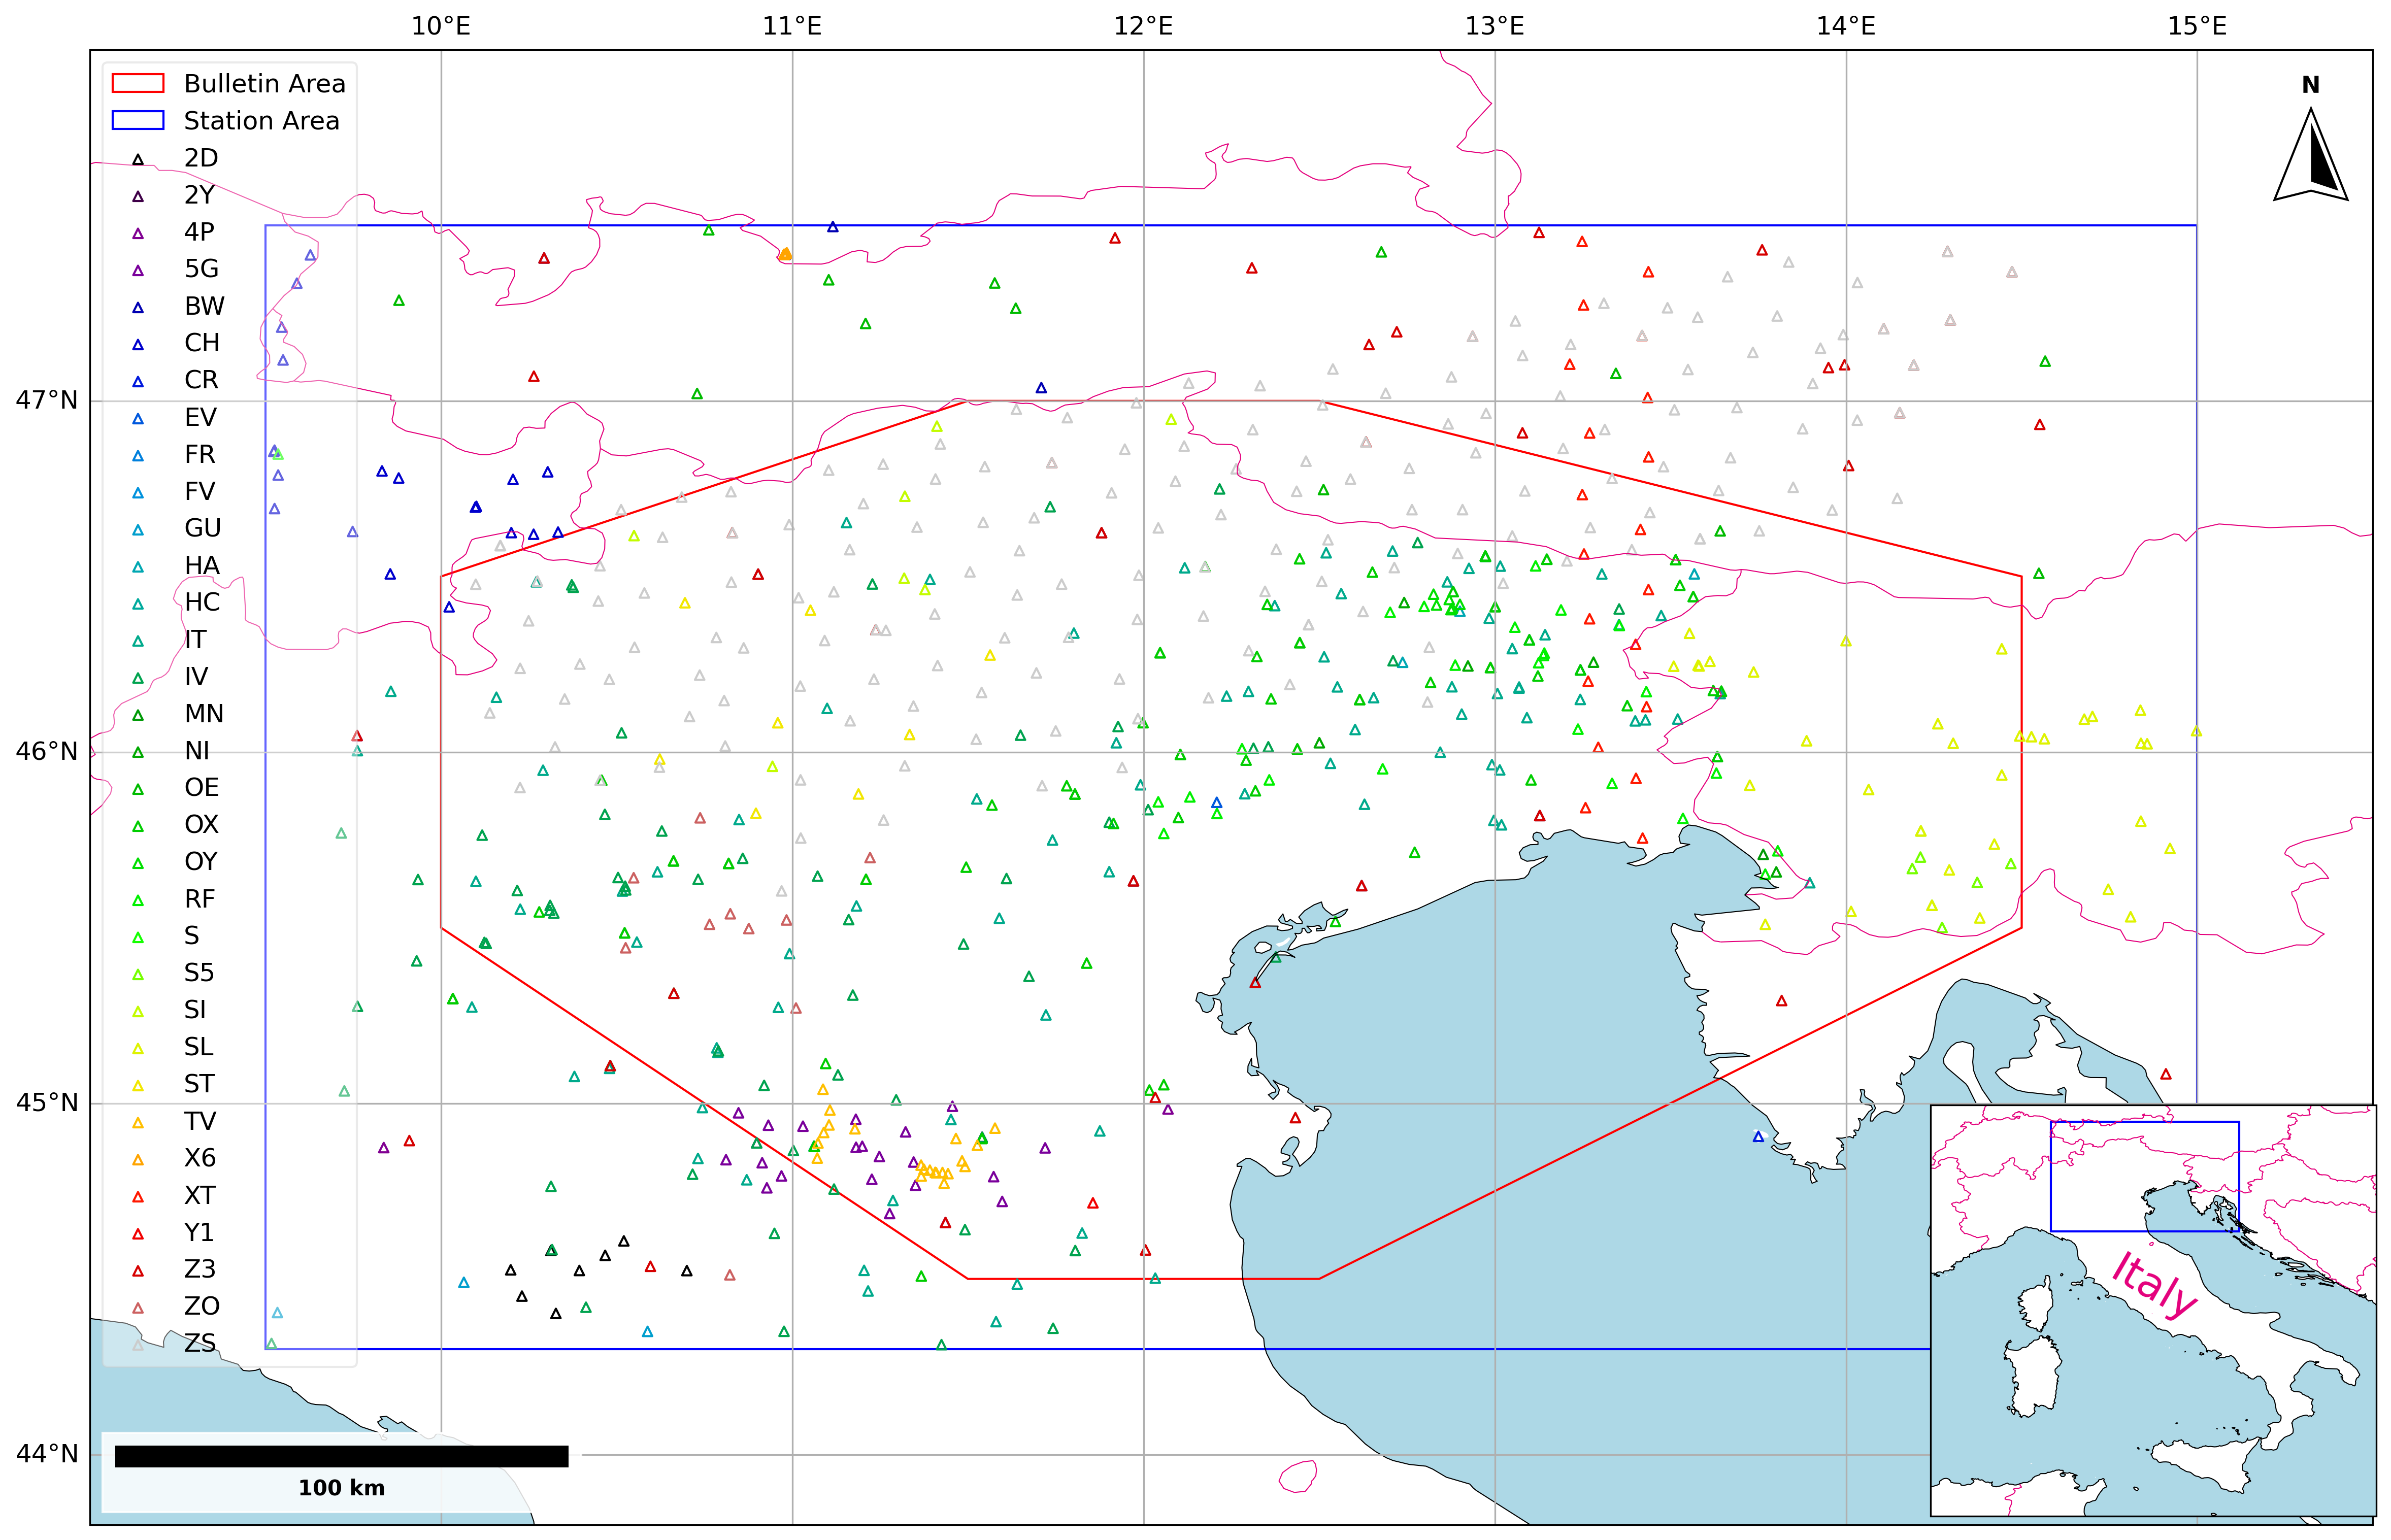
\includegraphics[width=\textwidth]{OGS/ALL/OGSStations.png}
  \caption{Spatial distribution of the 266 seismological and
    accelerometric stations across Northeastern Italy and adjacent
    border regions analyzed in this study. The reader should notice
    the high station density along the Friuli Prealpine belt and the
    transboundary coverage extending into Austria, Slovenia, and the
    Veneto plain. Station coordinates and metadata verified against
  official \ac{FDSN} StationXML inventories from 18 participating networks.}
  \label{fig:ogs_stations}
\end{figure}

\begin{figure}[htbp]
  \centering
  \MissingFigure{The event-map asset required for this figure is not present in
    the repository. A station-distribution map must not be substituted for an
    event-location map. Provide a versioned event-map artifact and its
    generating command before publication.
  }
  \caption{Placeholder for the event-location map within the \ac{OGS}
    operational polygon over the stated observation interval. The
    intended analysis is the spatial relation between analyst-curated
    reference events and the Socchieve sequence; no such relation is
    asserted while the map artifact is unavailable. Evidence
    limitation: the required versioned event-map file and its run
  provenance are absent from this checkout.}
  \label{fig:ogs_seismicity}
\end{figure}

\begin{figure}[htbp]
  \centering
  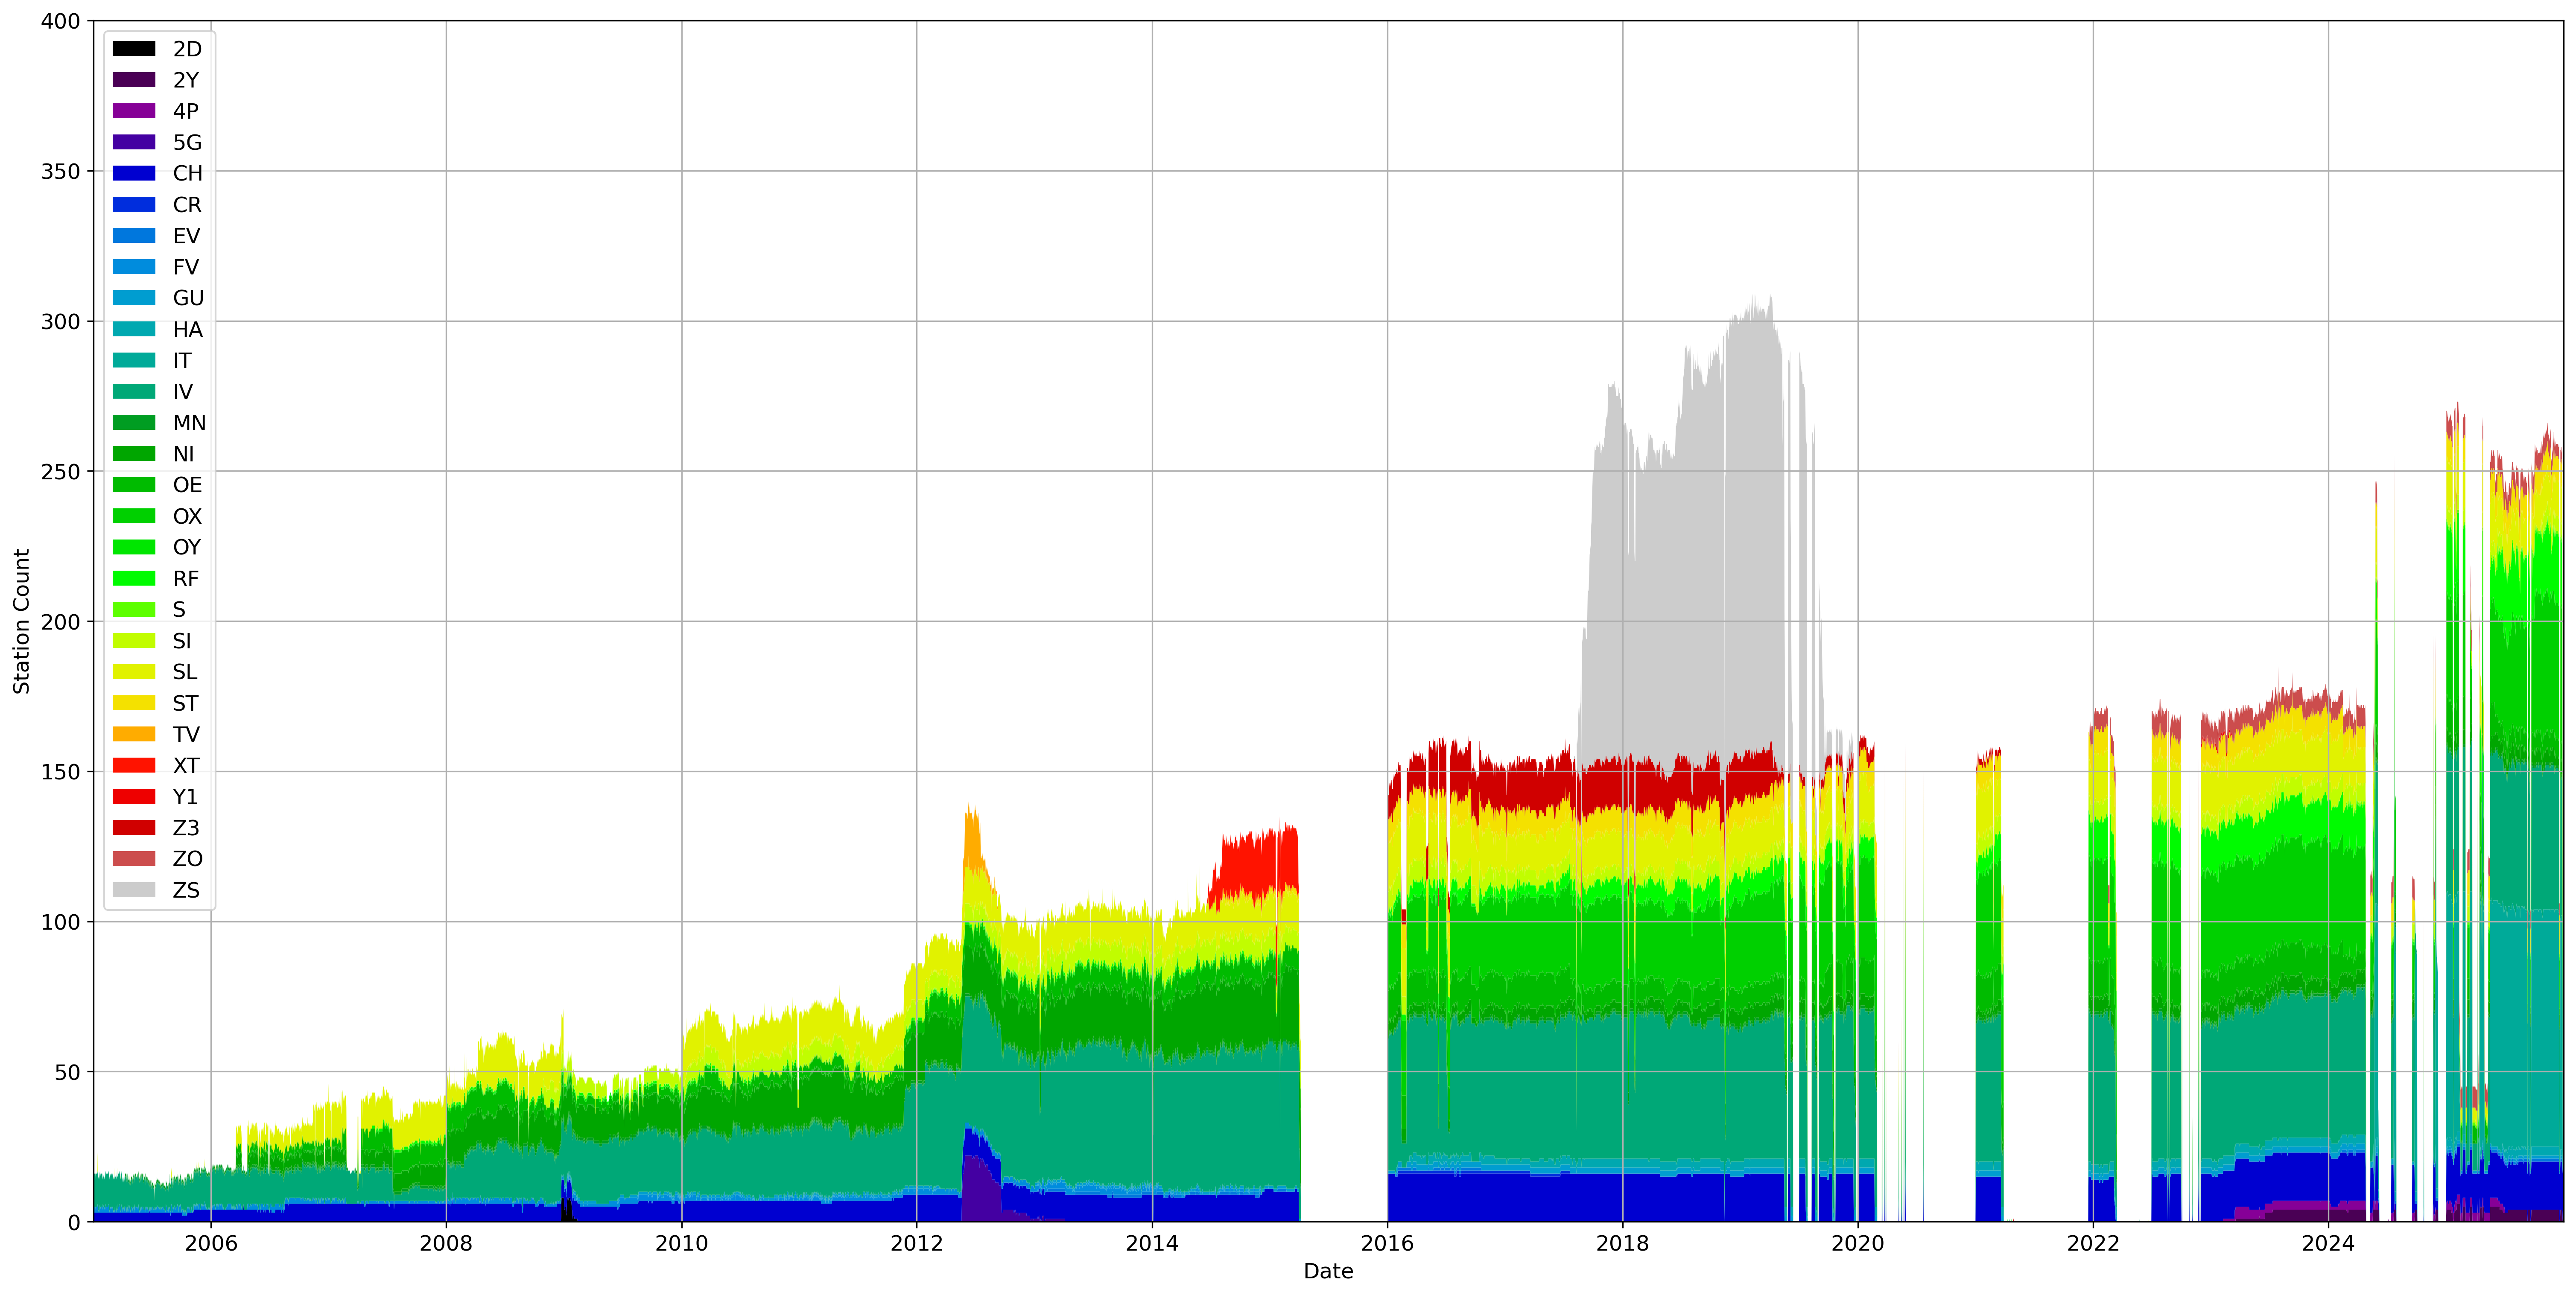
\includegraphics[width=\textwidth]{OGS/ALL/OGSAvailability.png}
  \caption{Temporal station availability and daily trace acquisition metrics
    across the regional network. The reader should notice the sustained
    operational continuity across participating networks, with minor transient
    drops resolved via automatic multi-client \ac{FDSN} fallback. Comprehensive
    annual station availability distributions covering the complete +20 years
    observational baseline (January 1st, 2005 to December 31st, 2025) across
    all 21 calendar years are detailed in Supplementary
    Material~\ref{sec:supp_annual_ogs_network}. Data generated from
    continuous miniSEED audit logs parsed by \texttt{ogsutils.waveforms}.
  }
  \label{fig:ogs_availability}
\end{figure}

\subsection{Analyst-Curated \ac{OGS} Reference Catalog}
\label{subsec:ogs_ground_truth}

To establish a baseline reference for evaluating the \ac{ML} pipeline,
we used an analyst-curated subset of the revised \ac{OGS} \acf{CRS} seismic
bulletin catalog \textcite{MagrinEtAl2026RevisedOGSCatalog}. The archive is a
reviewed operational reference, not an observation of every physical
earthquake. In standard operational practice, \ac{OGS} seismic analysts
manually pick phase arrivals, assign onset quality weights (see
Table~\ref{tab:h71_weights}), verify event associations, and compute
event hypocenters using Hypo71 or HypoEllipse algorithms. The source files
used here in the supported \texttt{.hpl}, \texttt{.dat}, \texttt{.txt}, and
\texttt{.pun} formats were parsed and merged by the \texttt{DataCatalog}
implementation in \path{OGS/src/ogsparser.py}; its output is a consolidated
catalog of standardized \texttt{EVENTS} and \texttt{PICKS} tables.

However, comparing \ac{ML} hypocenter locations derived
from modern probabilistic non-linear search algorithms against
legacy Hypo71 locations would introduce systematic biases arising
from differing inversion formulations, crustal velocity
discretizations, and station elevation corrections. Therefore, to
isolate the performance of the \ac{ML} picking and
association components, the \ac{OGS} reference events were independently
relocated using the identical \textbf{1D \acf{NonLinLoc}} velocity model and
inversion parameterization employed in our computational pipeline (Magrin,
personal communication).

The resulting relocated \ac{OGS} reference catalog contains:
\begin{itemize}
  \item \textbf{\placeholder{NUM EVENTS} confirmed seismic events} strictly
    contained within the regional polygon boundary \texttt{OGS\_POLY\_REGION}
    during the +20-year observation window (January 1st, 2005 to December 31st,
    2025).
  \item Local magnitudes ranging continuously from microseismic events
    ($M_{\mathrm{L}} = -0.2$) up to the $M_{\mathrm{L}}~4.6$ Socchieve
    mainshock, with completeness threshold $M_{\mathrm{c}} \approx 1.2$.
  \item Focal depths predominantly confined between $\qty{5.0}{\kilo\meter}$
    and $\qty{14.0}{\kilo\meter}$, reflecting the shallow seismogenic brittle
    layer of the Southern Alps.
  \item \textbf{\placeholder{NUM PICKS} manually verified phase picks},
    comprising \textbf{\placeholder{NUM P PICKS} Primary (P)} wave arrivals and
    \textbf{\placeholder{NUM S PICKS} Secondary (S)} wave arrivals. Each pick
    includes analyst-assigned onset polarity, weight, and timing uncertainty.
\end{itemize}

This high-quality reference catalog provides the baseline for the
bipartite graph matching assessment (\ac{BPGMA}) developed in
Chapter~\ref{chap:pipeline_evaluation}.

\section{Benchmark Machine-Learning Training Datasets}
\label{sec:benchmark_datasets}

The deep-learning phase pickers evaluated in this thesis—PhaseNet
and \ac{EQT}—rely on supervised training over massive
corpora of three-component seismic waveforms labeled with expert
ground-truth P- and S-wave arrival times. To understand how models
generalize across varying tectonic regimes and noise backgrounds, we
selected four benchmark datasets available through the SeisBench
framework \parencite{SeisBench}. Each dataset represents a distinct
combination of scale, geographical setting, instrumentation density,
and labeling curation.

\subsection{INSTANCE: The Italian Seismic Dataset for Machine Learning}
\label{subsec:instance}

The \acf{INSTANCE} dataset is a comprehensive open-access collection of labeled
seismic waveforms recorded across the Italian peninsula between 2005 and 2020
by the National Seismic Network (RSN), operated by \ac{INGV}, and partner
regional networks including \ac{OGS}.

Unlike global machine-learning datasets curated primarily for high \ac{SNR},
\ac{INSTANCE} was specifically designed to preserve the realistic operational
conditions of active regional monitoring networks:
\begin{itemize}
  \item \textbf{Operational Noise Realism}: \ac{INSTANCE} incorporates
    the full spectrum of environmental, cultural, and industrial
    noise characteristic of the Mediterranean and Alpine
    environments. This includes industrial vibrations, heavy road
    and rail traffic, quarry blasts, severe meteorological noise,
    and coastal microseisms.
  \item \textbf{Emergent and Low-Magnitude Arrivals}: The dataset
    encompasses a large proportion of small-magnitude events
    ($M_{\mathrm{L}} < 2.5$) exhibiting emergent onsets, complex
    scattering, and low signal-to-noise ratios.
  \item \textbf{Volume and Balance}: \ac{INSTANCE} comprises nearly
    \textbf{1.3 million three-component waveform traces}
    (\num{1291537}), including \num{1159249} labeled P-wave arrivals,
    \num{713883} labeled S-wave arrivals, across \num{54008} distinct events,
    and a dedicated negative class of \num{132288} pure noise windows
    extracted during periods without seismic activity.
  \item \textbf{Geographical Proximity}: Because \ac{INSTANCE} waveforms
    originate from Italy, the training wavefields reflect crustal attenuation,
    complex fault structures, and station vault installations physically
    similar to those of our Northeastern Italy study area.
\end{itemize}

\begin{figure}[htbp]
  \centering
  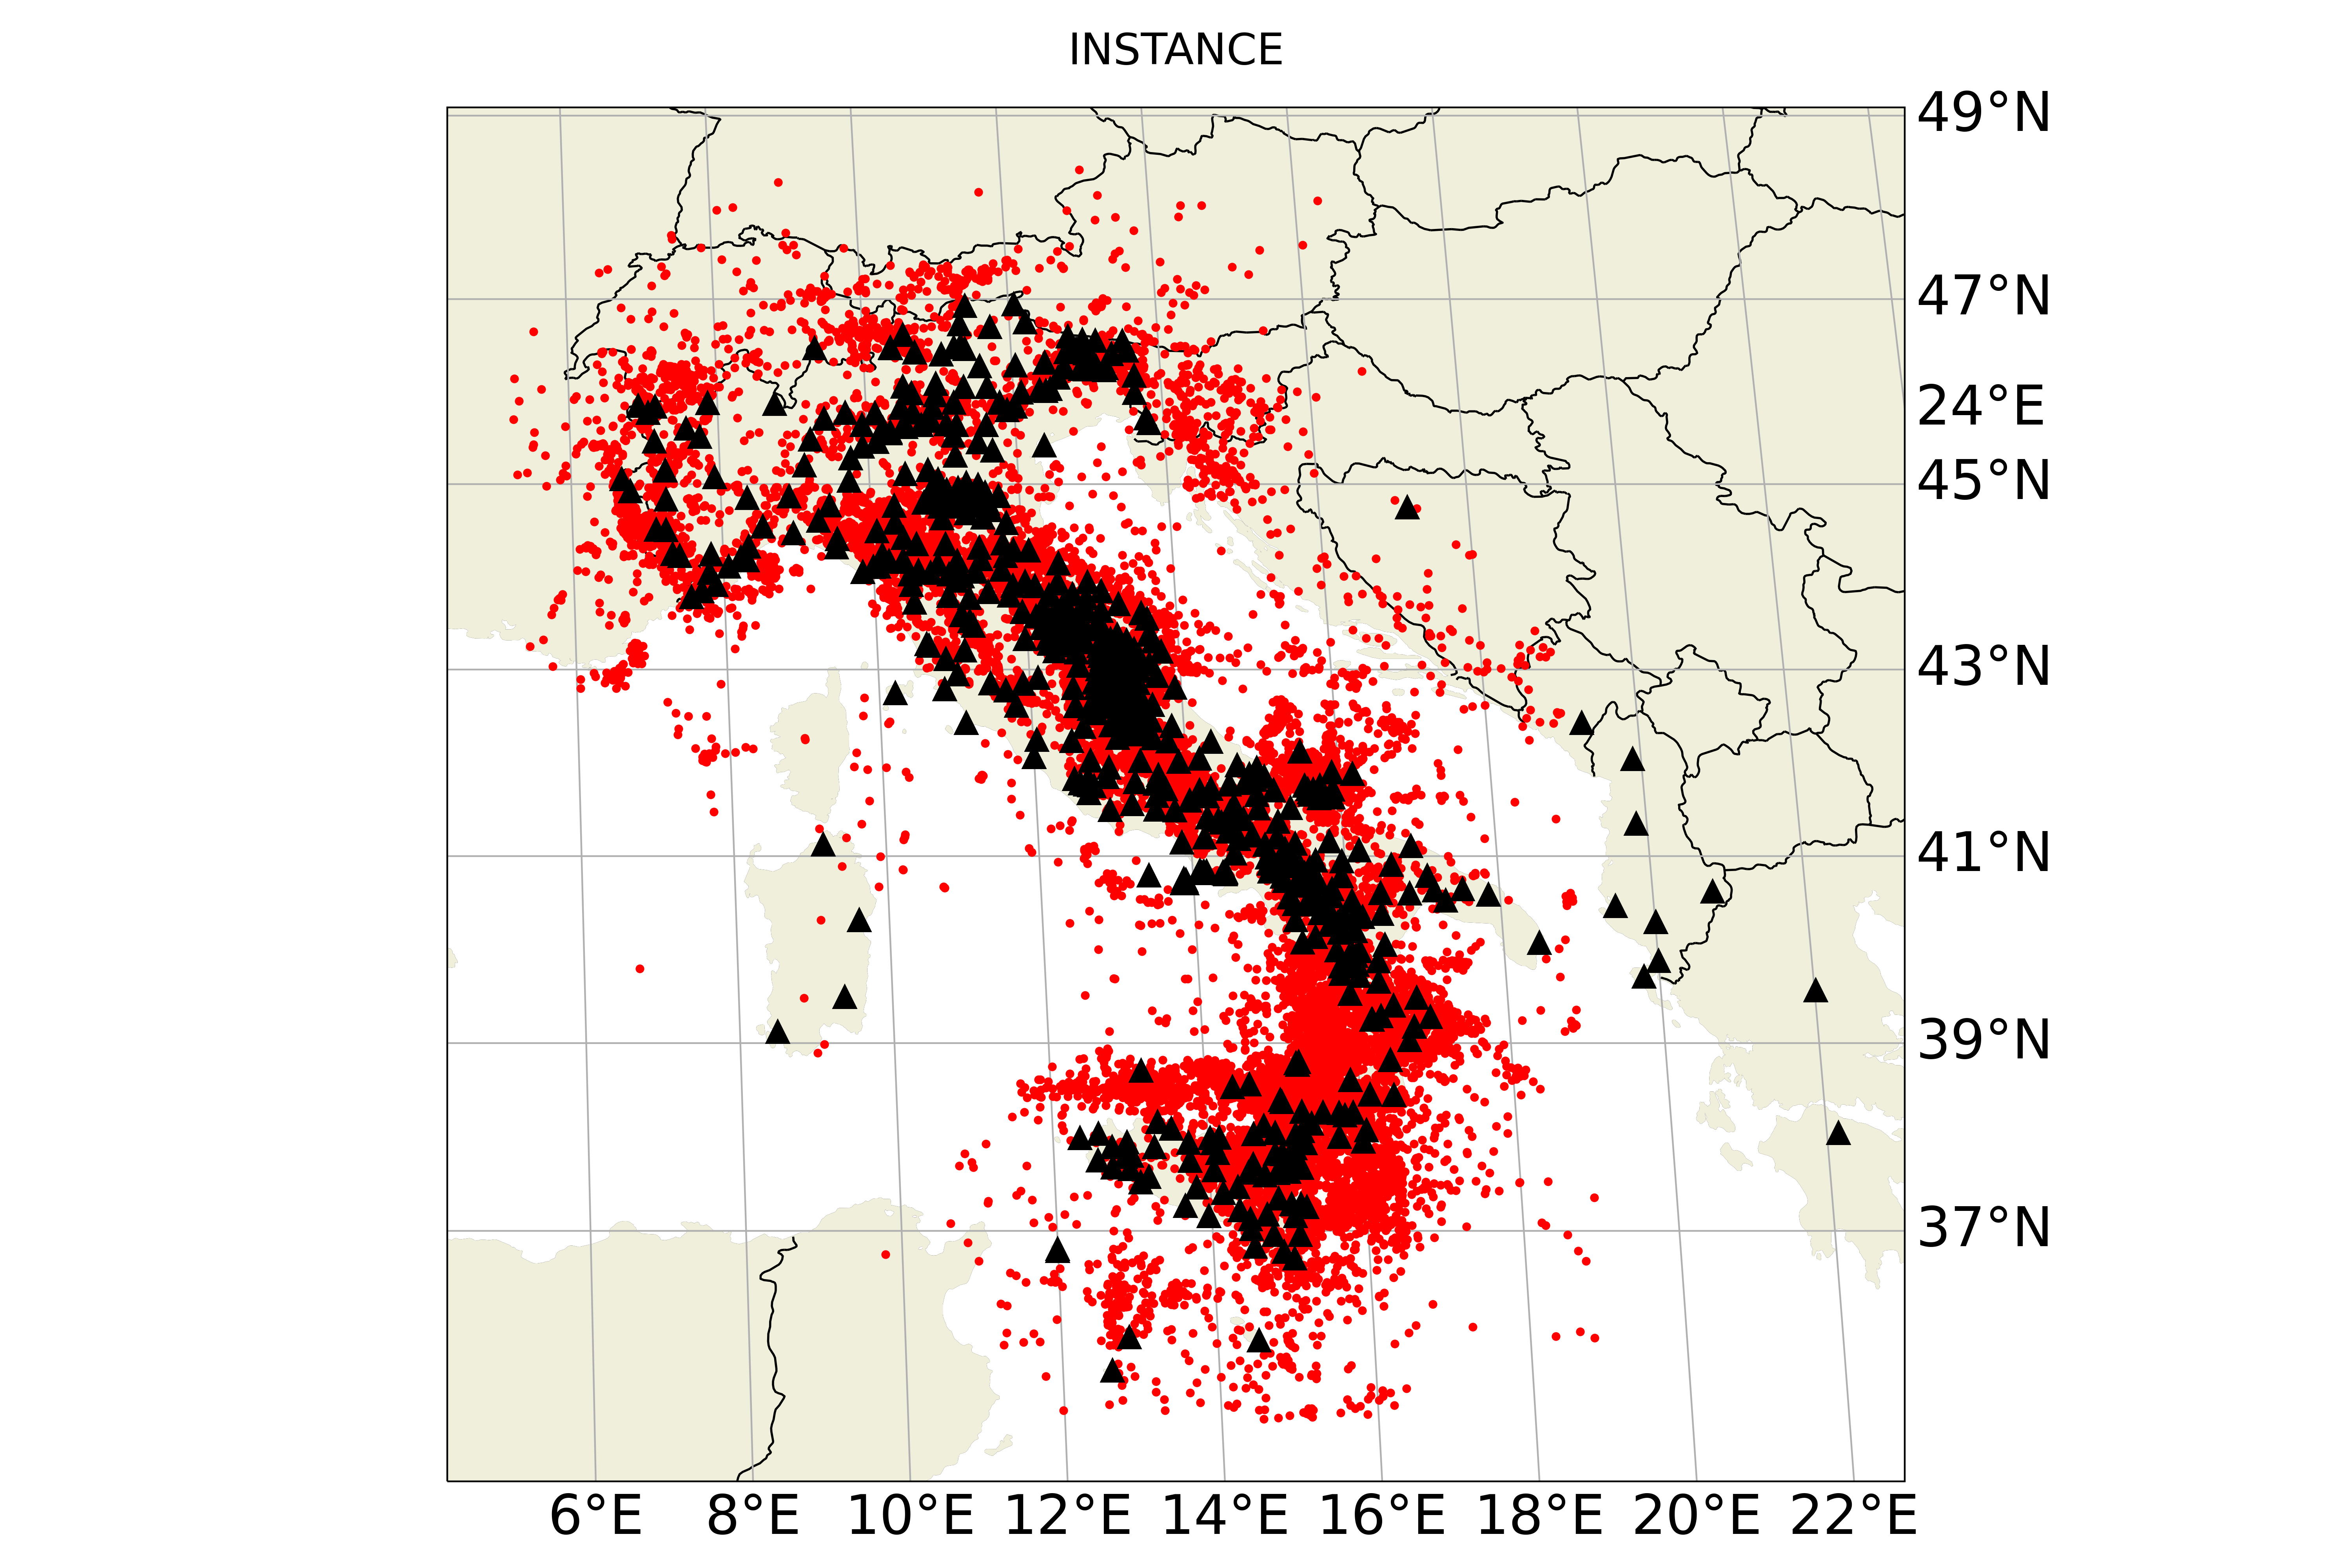
\includegraphics[width=0.82\textwidth]{INSTANCE.png}
  \caption{Geographical station distribution and event density of the
    \ac{INSTANCE} benchmark dataset across Italy. Notice the
    extensive coverage along the Apenninic chain and the
    Southern Alpine arc, capturing realistic Mediterranean crustal
    paths and anthropogenic noise conditions. Image taken from
  \textcite{SeisBench}.}
  \label{fig:instance_sample}
\end{figure}

\subsection{STEAD: STanford EArthquake Dataset}
\label{subsec:stead}

The \acf{STEAD} dataset \parencite{STEAD} is a globally distributed
benchmark dataset curated by researchers at Stanford University to
facilitate artificial intelligence research in seismology. Sourced
from seismic stations worldwide, \ac{STEAD} incorporates waveforms from
subduction zones, continental collision zones, volcanic systems, and
oceanic intraplate environments.

Key characteristics of \ac{STEAD} include:
\begin{itemize}
  \item \textbf{High Signal Clarity and Curation}: Waveforms were
    subjected to strict automated and manual quality filters,
    ensuring distinct wavefield onsets and elevated signal-to-noise
    ratios for earthquake signals.
  \item \textbf{Extensive Labeling}: \ac{STEAD} contains over
    \textbf{1.26 million three-component traces} (\num{1265657}), with
    \num{1030231} P-wave picks and \num{1030231} S-wave picks across
    \num{441705} distinct earthquakes.
  \item \textbf{Dedicated Noise Partition}: The dataset includes
    \num{235426} continuous noise recordings sampled across global
    stations, allowing neural networks to learn robust
    discriminative boundaries between non-stationary environmental
    noise and true seismic arrivals.
  \item \textbf{Global Transferability}: By encompassing a wide
    variety of sensor types, crustal velocity structures, and
    epicentral distances (local to regional, up to
    $\qty{350}{\kilo\meter}$), \ac{STEAD} is engineered to prevent models from
    overfitting to region-specific propagation paths.
\end{itemize}

\begin{figure}[htbp]
  \centering
  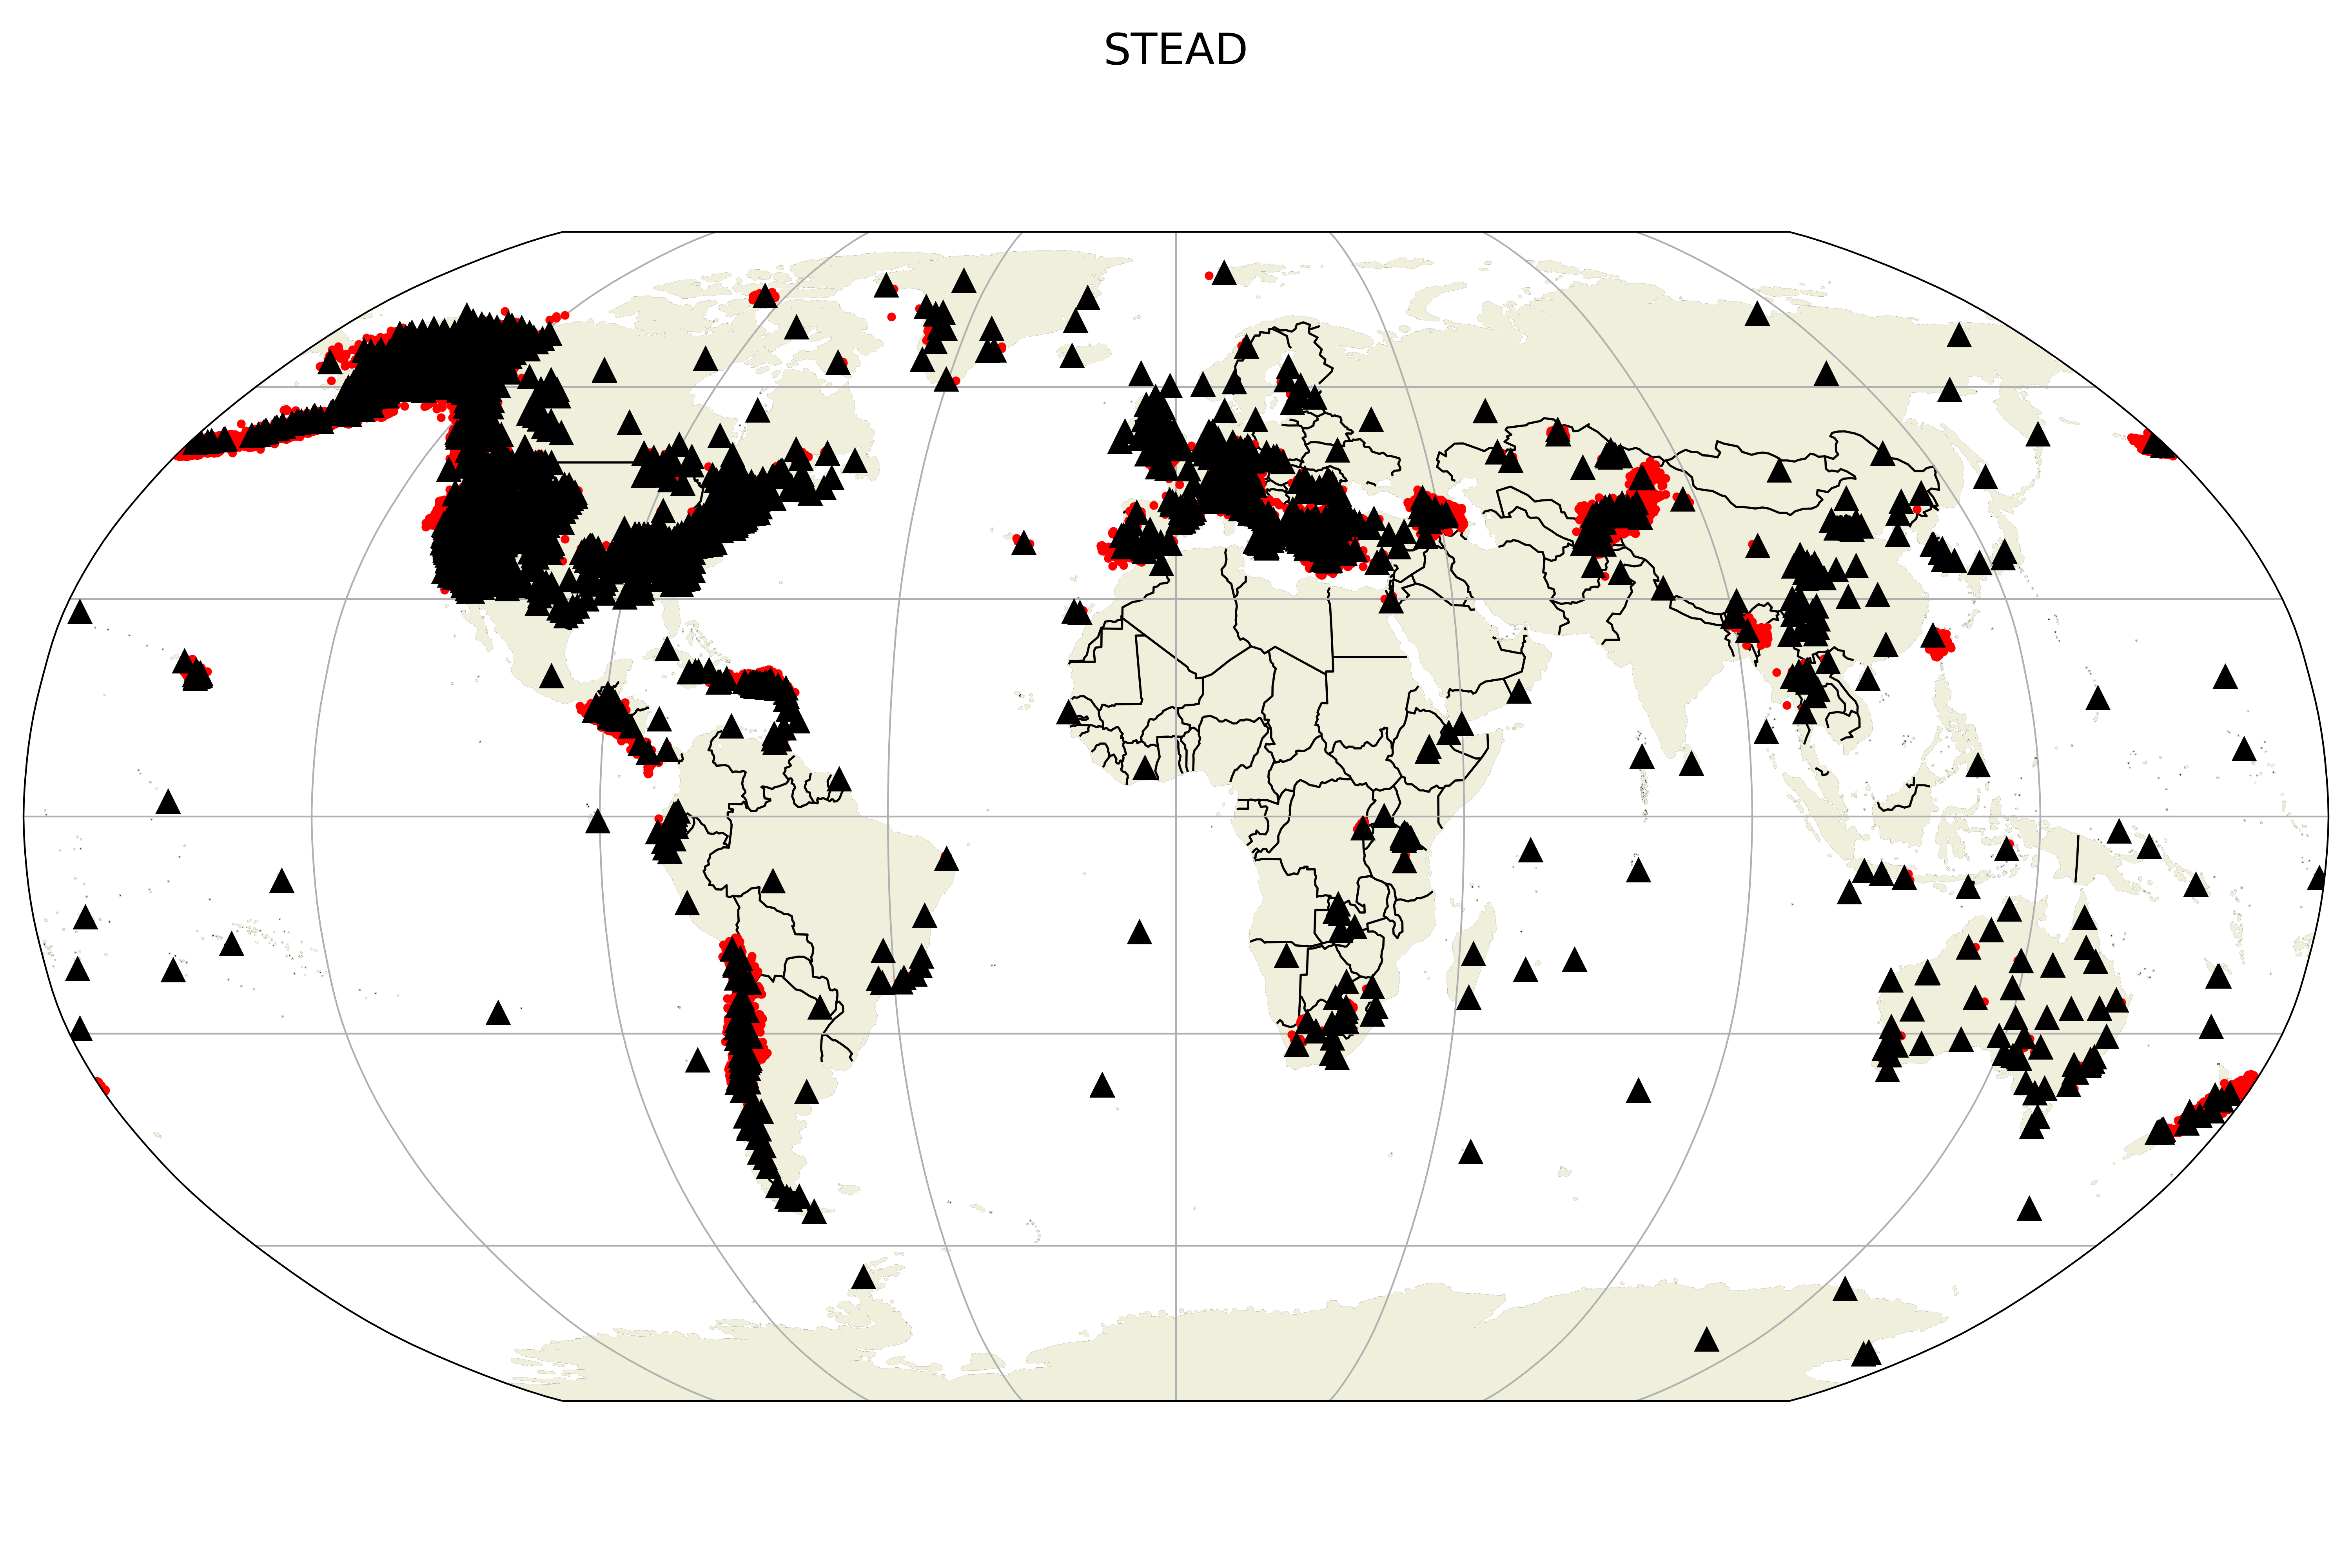
\includegraphics[width=0.82\textwidth]{STEAD.png}
  \caption{Worldwide distribution of seismological stations contributing
    waveform recordings to the global \ac{STEAD} benchmark dataset. The reader
    should notice the broad geographic and tectonic representation across
    diverse orogenic belts and plate boundaries. Image taken from
    \textcite{SeisBench}.
  }
  \label{fig:stead_sample}
\end{figure}

\subsection{SCEDC: Southern California Earthquake Data Center}
\label{subsec:scedc}

The \acf{SCEDC} dataset \parencite{SCEDC} provides an unprecedented
volume of seismic recordings curated from the \acf{SCSN}, spanning decades
of continuous monitoring across the San Andreas fault system.

\ac{SCEDC} is characterized by:
\begin{itemize}
  \item \textbf{Massive Data Volume}: Sourced through SeisBench, the
    \ac{SCEDC} dataset contains \textbf{8.11 million three-component
    traces} (\num{8111060}), incorporating \num{7571970} P-wave picks
    and \num{4364155} S-wave picks across \num{378528} local earthquakes.
  \item \textbf{Dense Local Network Geometry}: The \ac{SCSN} features an
    exceptionally high spatial sensor density, capturing
    high-frequency wavefield details over purely local propagation
    paths ($\Delta \le \qty{150}{\kilo\meter}$).
  \item \textbf{Catalog Completeness}: Decades of continuous analyst
    curation and automated cross-correlation template matching make
    the \ac{SCEDC} catalog complete to very low magnitude thresholds
    ($M_{\mathrm{c}} \approx 1.0$), minimizing missing pick
    annotations in the training labels.
  \item \textbf{Regional Bias}: While mathematically advantageous
    for training deep high-capacity networks with millions of
    parameters without overfitting, the dataset is geographically
    homogeneous, reflecting Southern California crustal velocity
    gradients and strike-slip tectonic structures.
\end{itemize}

\begin{figure}[htbp]
  \centering
  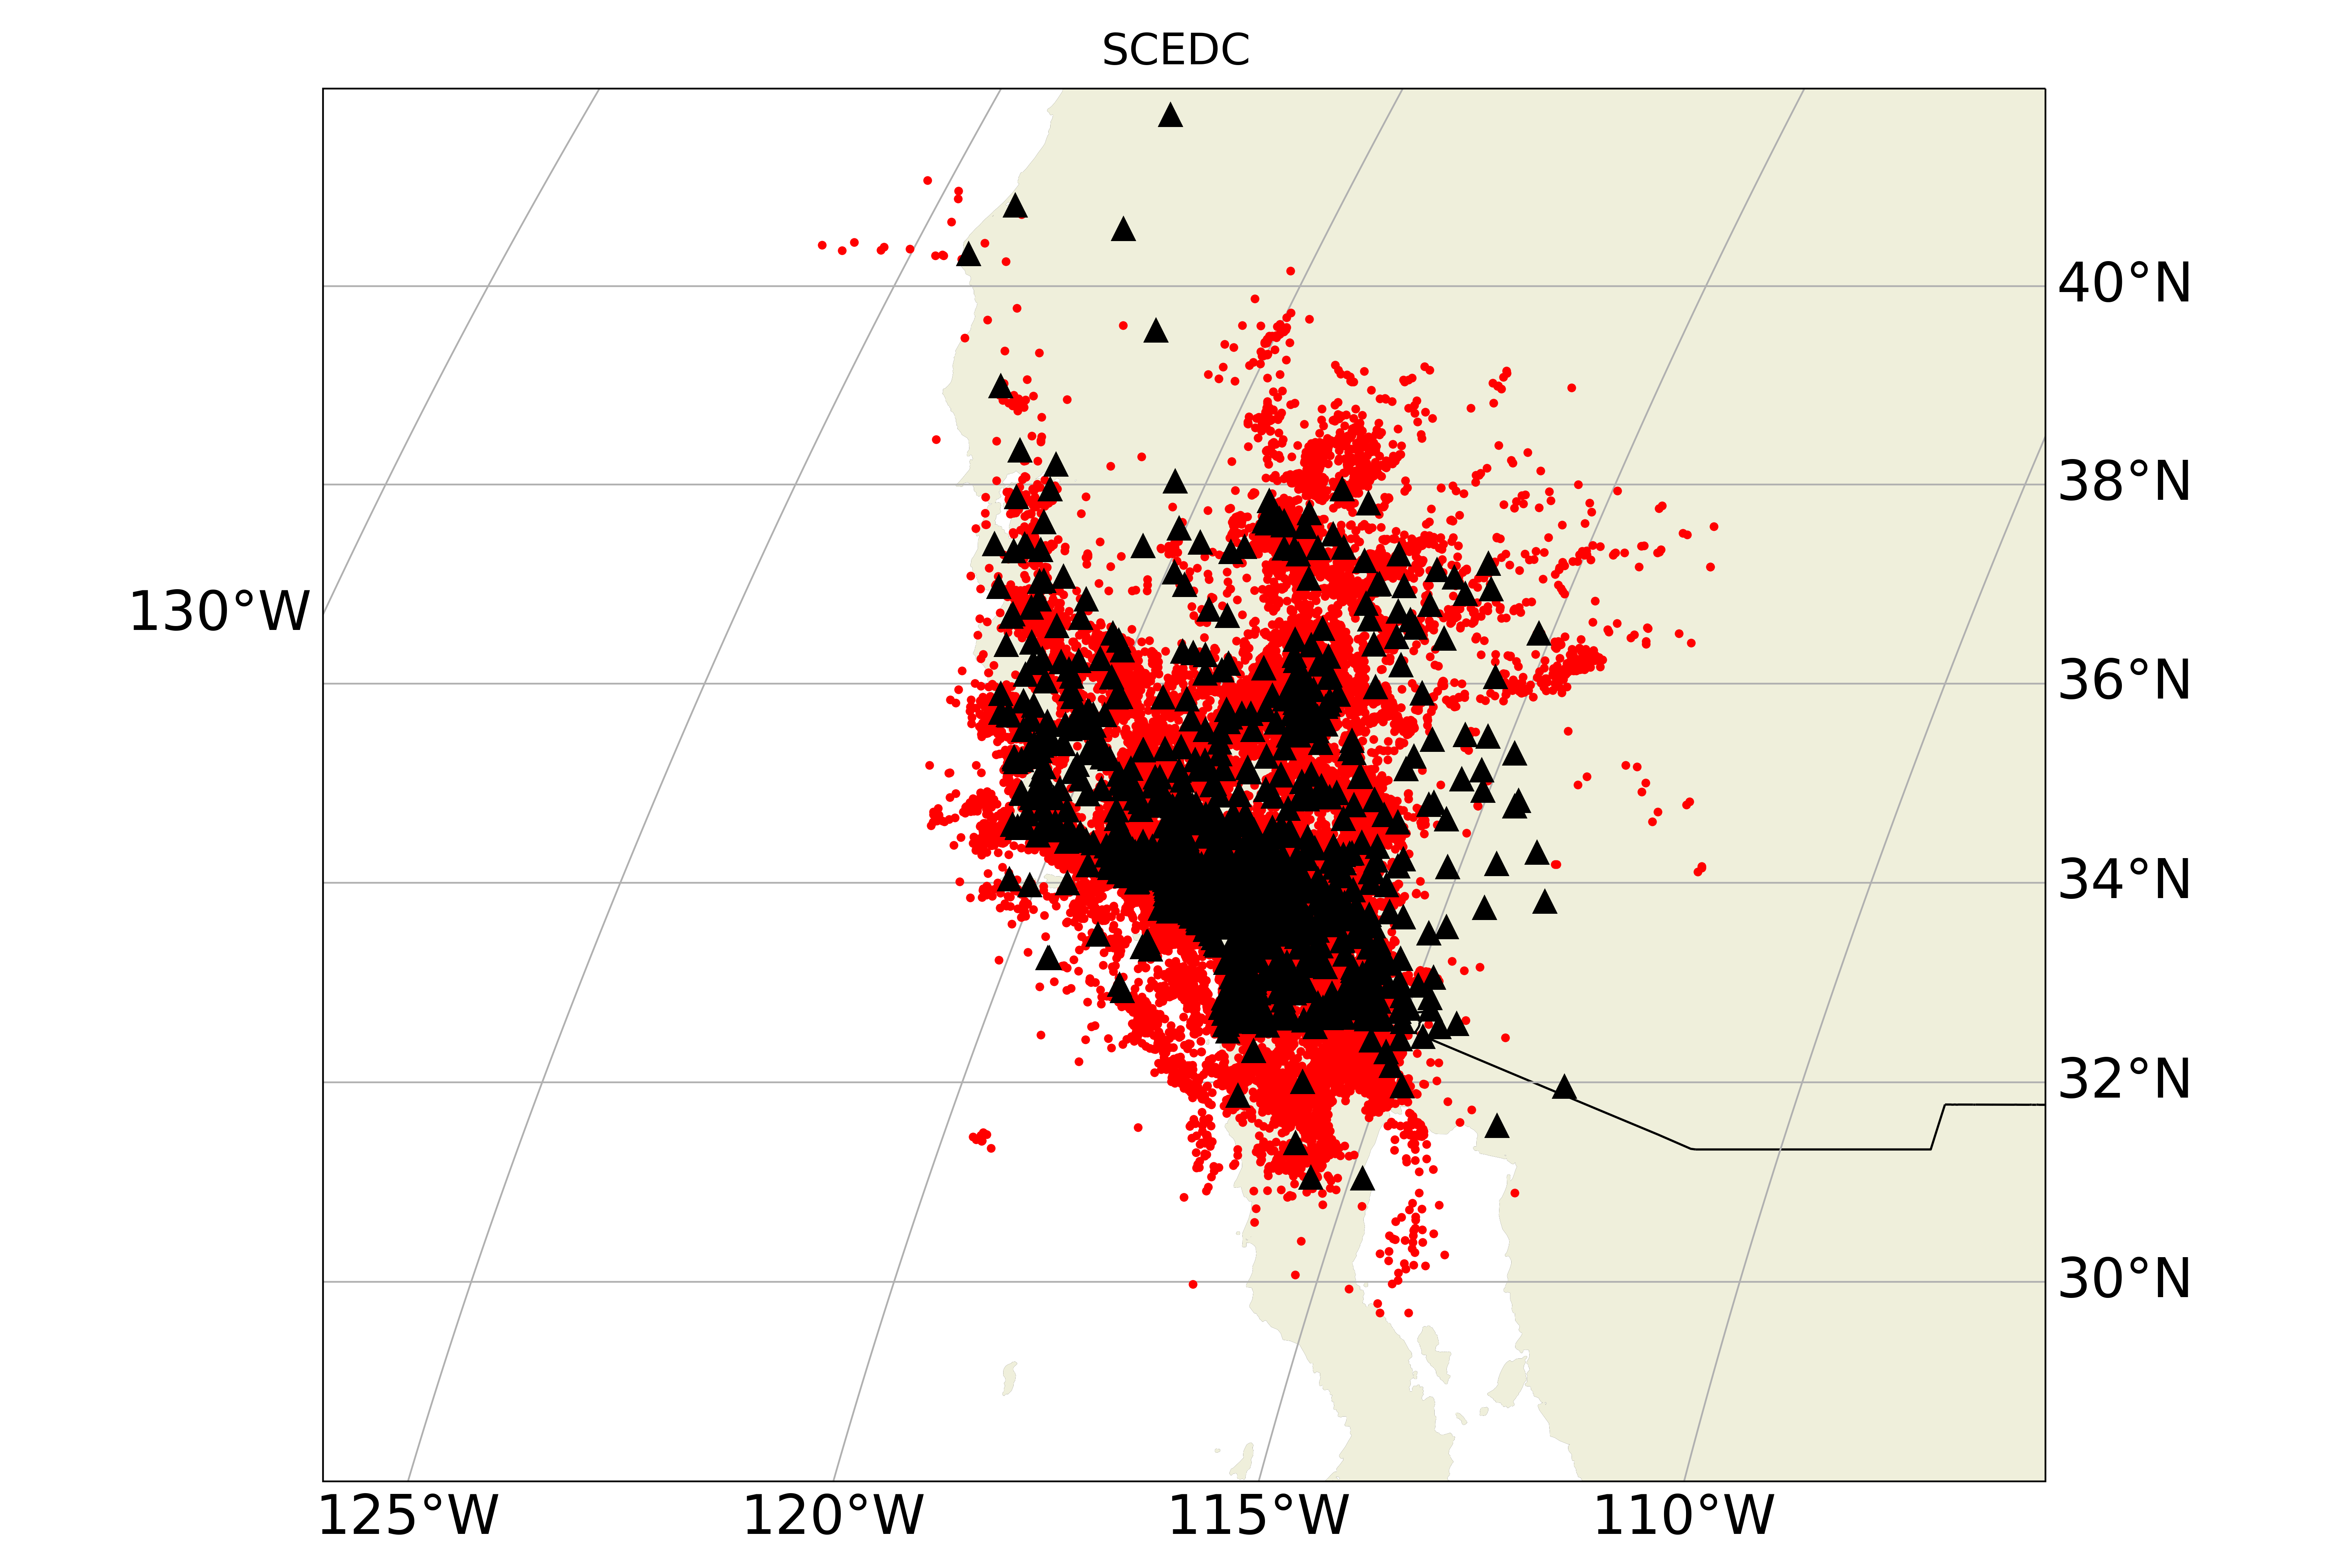
\includegraphics[width=0.82\textwidth]{SCEDC.png}
  \caption{Spatial station distribution of the \ac{SCSN} represented
    in the \ac{SCEDC} dataset. The
    reader should notice the dense spatial grid concentrated along the
    San Andreas fault system and the Los Angeles basin. Image
  taken from \textcite{SeisBench}.}
  \label{fig:scedc_sample}
\end{figure}

\subsection{Original Author Dataset: PhaseNet and EQTransformer}
\label{subsec:original_corpora}

In addition to the three standard community benchmark datasets, we
evaluate the models trained on the original datasets established by
the respective model architects:
\begin{itemize}
  \item \textbf{Original \ac{PhaseNet} Dataset} \parencite{PhaseNet}: Curated
    by the \ac{NCSN}, this dataset
    comprises approximately $779,514$ waveform traces recorded
    across $234,117$ local seismic events in Northern California.
    The dataset features high-quality manual analyst arrival times
    but lacks explicitly segregated noise-only windows, relying
    instead on pre-onset waveform segments to represent ambient noise.
  \item \textbf{Original \ac{EQT} Dataset}
    \parencite{EQTransformer}: Curated as a specialized subset of the
    \ac{STEAD} repository, comprising approximately $1.2$ million
    three-component traces selected to optimize multi-task
    transformer training for simultaneous earthquake detection, P
    picking, and S picking across \qty{60}{\second} waveform windows.
\end{itemize}

\section{Synthesis of Benchmark Datasets and Methodological Comparison}
\label{sec:dataset_synthesis}

Table~\ref{tab:datasets} provides a rigorous, publication-grade
comparative synthesis of all benchmark datasets utilized in this
thesis. All datasets share a common sampling frequency of
$\qty{100}{\hertz}$, either natively or through standardized
SeisBench decimation, ensuring absolute tensor dimensionality
consistency across all deep-learning inference workflows.

\begin{table}[htbp]
  \centering
  \small
  \caption{Systematic comparison of seismological benchmark training
    datasets used for PhaseNet and EQTransformer models. The reader
    should notice the substantial contrast between the massive sample
    volume of SCEDC and the balanced regional noise realism of
    \ac{INSTANCE}. Traces, noise windows, and pick counts are derived from
    SeisBench metadata schemas; distance bounds classify local
    ($\Delta \le \qty{150}{\kilo\meter}$) versus regional ($150 < \Delta \le
  \qty{600}{\kilo\meter}$) propagation paths.}
  \label{tab:datasets}
  \begin{threeparttable}
    \begin{tabularx}{\linewidth}{l r r r r c l}
      \toprule
      \textbf{Dataset} & \textbf{Traces} & \textbf{P Picks} &
      \textbf{S Picks} & \textbf{Events} & \textbf{Noise Traces} &
      \textbf{Coverage / Dist.\tnote{a}} \\
      \midrule
      \ac{INSTANCE} & \num{1291537} & \num{1159249} &
      \num{713883} & \num{54008} & \num{132288} & Italy (L / R) \\
      \ac{STEAD}    & \num{1265657} & \num{1030231} &
      \num{1030231} & \num{441705} & \num{235426} & Global (L / R) \\
      \ac{SCEDC}    & \num{8111060} & \num{7571970} &
      \num{4364155} & \num{378528} & \num{0}\tnote{b} & S. California (L) \\
      \ac{PhaseNet}\tnote{c} & \num{779514} &
      \multicolumn{2}{c}{--- \tnote{d} ---} & \num{234117} &
      \num{0}\tnote{b} & N. California (L) \\
      \ac{EQT}\tnote{c} & \num{1200000} & \num{1000000}
      & \num{1000000} & \num{400000} & \num{200000} & Global (L / R) \\
      \bottomrule
    \end{tabularx}
    \begin{tablenotes}[flushleft]
      \footnotesize
    \item[a] Epicentral distance classification: Local
      ($\mathrm{L}$) denotes $\Delta \le \qty{150}{\kilo\meter}$; Regional
      ($\mathrm{R}$) denotes $\qty{150}{\kilo\meter} < \Delta \le
      \qty{600}{\kilo\meter}$.
    \item[b] Dedicated pure noise trace partitions were not
      independently generated in the \ac{SCEDC} and original \ac{PhaseNet}
      repositories; ambient noise representations are extracted from
      pre-P arrival waveform windows.
    \item[c] Original \ac{PhaseNet} and \ac{EQT} datasets as described in their
      respective publications.
    \item[d] In the original \ac{PhaseNet} publication \parencite{PhaseNet},
      separate counts for P and S arrivals were not reported
      individually; both phase classes are present in the labeled
      training windows.
    \end{tablenotes}
  \end{threeparttable}
\end{table}

\subsection{The Domain Adaptation Hypothesis}
\label{subsec:domain_adaptation_hypothesis}

A central scientific question explored in this dissertation is the
\textbf{domain adaptation hypothesis}: does a deep neural network
trained on massive volumes of data from a distant geological setting
(such as the 8.1 million traces of \ac{SCEDC} in Southern California)
outperform a network trained on a smaller but regionally congruent
dataset (such as the 1.3 million traces of \ac{INSTANCE} in Italy)?

In classical supervised machine learning, statistical theory assumes
that training and testing samples are identically and independently
distributed ($i.i.d.$) from the same underlying probability distribution:
\begin{equation}
  P_{\mathrm{train}}(\mathbf{X}, \mathbf{Y}) =
  P_{\mathrm{test}}(\mathbf{X}, \mathbf{Y}).
  \label{eq:iid_assumption}
\end{equation}
In operational seismology, this assumption is fundamentally violated
when transferring models across geographical regions
($P_{\mathrm{train}} \neq P_{\mathrm{test}}$). Regional differences include:
\begin{enumerate}
  \item \textbf{Path Effects and Velocity Dispersions}: Distinct
    crustal velocity gradients, Conrad/Moho discontinuity depths,
    and intrinsic attenuation ($Q$-factor) modify wavefield
    dispersion and P-to-S coda energy ratios.
  \item \textbf{Anthropogenic and Environmental Noise Spectra}:
    Cultural noise in densely populated European valleys
    (characterized by \qty{50}{\hertz} electrical harmonics, narrow road
    networks, and industrialized river plains) differs substantially
    from noise in the Mojave desert or Southern California coastal basins.
  \item \textbf{Instrumental Hardware Responses}: Variations in
    sensor eigenfrequencies, digitizer bit depths, and vault
    coupling introduce subtle spectral colorations into the
    digitized waveforms.
\end{enumerate}

By systematically evaluating \ac{PhaseNet} and \ac{EQT} models
trained across \ac{INSTANCE}, \ac{STEAD}, \ac{SCEDC}, and the
original datasets on
the identical three-month \ac{SMINO} continuous dataset, this study
provides empirical bounds on regional domain transferability
(presented in Chapter~\ref{chap:results}).

\supplementarymaterial{Datasets}{Datasets}

\chapter{Data Engineering}
% Purpose: Software architecture, central configuration, data acquisition,
% multi-format catalog parsing, aggregation, and visualization framework.
% Status: Draft; under academic review.
% Source-of-truth: OGS/src/ogsconstants.py, OGS/src/ogsdatafile.py,
% OGS/src/ogsparser.py, OGS/src/ogshpl.py, OGS/src/ogsdat.py,
% OGS/src/ogstxt.py, OGS/src/ogspun.py, OGS/src/ogsdownloader.py,
% OGS/src/ogsplotter.py, OGS/src/ogsutils.py

\label{chap:data_engineering}

The development and deployment of an automated, operational seismic catalog
pipeline requires a robust, scalable data engineering infrastructure.
Seismological observatories must routinely ingest heterogeneous multi-channel
continuous waveforms from distributed networks, parse decades of legacy catalog
archives stored in idiosyncratic text formats, merge multi-source hypocenter
and magnitude solutions, and render high-resolution geographic and statistical
visualizations.

This chapter details the data engineering framework developed for this
dissertation, implemented as a modular Python package under \texttt{OGS/src/}.
\Cref{sec:software_architecture} presents the software design patterns
and the central configuration module \texttt{ogsconstants}.
\Cref{sec:weight_conversion} establishes the formal
weight-to-uncertainty mapping. \Cref{sec:data_acquisition} describes the
distributed \ac{FDSN} continuous waveform acquisition architecture.
\Cref{sec:catalog_parsing} formulates the extensible multi-format
catalog parsing hierarchy. \Cref{sec:catalog_aggregation} details the
automated format detection, merging logic, and columnar persistence.
\Cref{sec:visualization_framework} presents the object-oriented
visualization framework and geodetic math. Finally,
\cref{sec:storage_strategy} outlines the tiered storage strategy and
quality assurance protocols.

\section{Software Architecture and Central Configuration Module}
\label{sec:software_architecture}

The data engineering pipeline is architected around object-oriented and
functional programming paradigms in Python 3.12, interfacing with core
scientific computing libraries including NumPy \parencite{NumPy}, pandas
\parencite{McKinney2010,pandas}, ObsPy \parencite{ObsPy}, Pyrocko
\parencite{Pyrocko}, Cartopy \parencite{Cartopy}, and scikit-learn
\parencite{scikit-learn}. To ensure
maintainability, maintain loose coupling between processing stages, and
eliminate hardcoded parameters, the system adheres to the \textbf{Single
Source of Truth} design pattern. A comprehensive synthesis of the scientific
software stack, respective environment versions, formal citations, and
operational scopes is presented in \cref{tab:software_ecosystem}.

\begin{table}[htbp]
  \centering
  \small
  \caption{Core scientific computing libraries and software dependencies
    powering the seismological data engineering and analysis pipeline.
    Runtime specifications and versions correspond to the production \ac{HPC}
    environment \texttt{SBC\_3.12} (\texttt{OGS/utils/Leonardo/LEONARDO.yml}).
  }
  \label{tab:software_ecosystem}
  \begin{threeparttable}
    \begin{tabularx}{\linewidth}{l l l X}
      \toprule
      \textbf{Library / Tool} & \textbf{Version\tnote{a}} &
      \textbf{Citation} & \textbf{Operational Role in Pipeline} \\
      \midrule
      \texttt{Python} & \texttt{3.12.13} & --- & Core
      object-oriented runtime and execution environment \\
      \texttt{NumPy} & \texttt{2.4.2} & \textcite{NumPy} &
      $N$-dimensional array operations and vectorized calculations \\
      \texttt{SciPy} & \texttt{1.17.1} & \textcite{SciPy} &
      Scientific algorithms, spatial indices, and optimization \\
      \texttt{pandas} & \texttt{3.0.1} & \textcite{pandas} & Tabular
      catalog serialization and columnar Parquet I/O \\
      \texttt{ObsPy} & \texttt{1.4.2} & \textcite{ObsPy} & FDSN
      client access, MiniSEED parsing, and geodetic math \\
      \texttt{Pyrocko} & \texttt{2025.12.4} & \textcite{Pyrocko} &
      High-performance Squirrel day-sharded waveform storage \\
      \texttt{PyTorch} & \texttt{2.10.0} & \textcite{PyTorch} &
      GPU-accelerated neural network inference and training \\
      \texttt{SeisBench} & \texttt{0.11.0} & \textcite{SeisBench} &
      Benchmark loading, trace normalization, and model dispatch \\
      \texttt{scikit-learn} & \texttt{1.7.0} &
      \textcite{scikit-learn} & Evaluation metrics, confusion
      matrices, and bipartite matching \\
      \texttt{Cartopy} & \texttt{0.25.0} & \textcite{Cartopy} &
      Cartographic map projections and spatial region boundary rendering \\
      \texttt{Matplotlib} & \texttt{3.10.8} & \textcite{Matplotlib}
      & Publication-quality seismic charts, phase plots, and figures \\
      \texttt{Hydra} & \texttt{1.3.2} & \textcite{Hydra} &
      Hierarchical YAML configuration management and dynamic CLI overrides \\
      \bottomrule
    \end{tabularx}
    \begin{tablenotes}[flushleft]
    \item[a] Environment versions extracted from Conda specification
      \texttt{SBC\_3.12} on the Cineca Leonardo HPC platform.
    \end{tablenotes}
  \end{threeparttable}
\end{table}

\subsection{The Central Configuration Module: \texttt{ogsconstants}}
\label{sec:ogsconstants}

The \texttt{ogsconstants.py} module serves as the central configuration
repository for the entire codebase. Every pipeline stage—data downloading,
parsing, neural picking, phase association, relocation, magnitude estimation,
bipartite matching, and plotting—imports its operational constants, schema
definitions, regex fragments, and mathematical tolerances directly from this
module.

The primary configuration domains governed by \texttt{ogsconstants} include:
\begin{enumerate}
  \item \textbf{Parallel Execution and \ac{HPC} Hardware Allocation}:
    \begin{itemize}
      \item \texttt{MPI\_RANK}, \texttt{MPI\_SIZE},
        \texttt{MPI\_COMM}: Global variables capturing \acf{MPI} process rank,
        communicator size, and communicator topology for distributed multi-node
        execution on \ac{HPC} clusters.
      \item \texttt{GPU\_RANK}, \texttt{GPU\_SIZE}: Device identifiers managing
        \ac{CUDA} device affinity for multi-\ac{GPU} inference
        across NVIDIA Ampere A100 nodes.
      \item \texttt{EPSILON = 1e-6}: Small numerical constant preventing
        division-by-zero singularities during travel-time residual calculations
        and weight inversions.
    \end{itemize}

  \item \textbf{Standardized Date and Time Representations}:
    Seismological files and web services employ diverse date-time string
    conventions. The module defines canonical format strings following Python
    \texttt{strftime} standards:
    \begin{itemize}
      \item \texttt{DATE\_FMT = "\%Y-\%m-\%d"}: Standard ISO 8601 calendar
        date.
      \item \texttt{TIME\_FMT = "\%H\%M\%S"}: Compact six-digit time string.
      \item \texttt{YYMMDD\_FMT = "\%y\%m\%d"} and
        \texttt{YYYYMMDD\_FMT = "\%Y\%m\%d"}: Two-digit and four-digit year
        date representations.
      \item \texttt{DATETIME\_FMT = "\%y\%m\%d\%H\%M\%S"}: Compact
        twelve-digit timestamp string used in legacy fixed-width records.
      \item \texttt{ONE\_DAY = timedelta(days=1)}: Fundamental step interval
        for temporal partitioning.
    \end{itemize}

  \item \textbf{Phase Identifiers and Detection Thresholds}:
    \begin{itemize}
      \item \texttt{PWAVE = "P"}, \texttt{SWAVE = "S"}: Authoritative phase
        type string literals.
      \item \texttt{THRESHOLDS}: Systematic confidence threshold array spanning
        \numrange{0.1}{0.9} in increments of \num{0.1}, constructed via
        \texttt{np.linspace(0.1, 0.9, 9)}.
      \item \texttt{PWAVE\_THRESHOLD = SWAVE\_THRESHOLD = 0.1}: Default minimum
        model probability threshold (\num{0.1}) for accepting
        \ac{ML} phase candidates.
    \end{itemize}

  \item \textbf{Spatial Domain and Polygon Boundaries}:
    \begin{itemize}
      \item \texttt{OGS\_POLY\_REGION}: An eight-vertex convex
        polygon enclosing the core monitoring area in Northeastern
        Italy, defined by ordered $(lon, lat)$ coordinate pairs:
        \begin{equation}
          \begin{aligned}
            \mathcal{P}_{\mathrm{OGS}} \coloneqq \{ &(\ang{10.0},
              \ang{45.5}),\, (\ang{10.0}, \ang{46.5}),\,
              (\ang{11.5}, \ang{47.0}),\, (\ang{12.5}, \ang{47.0}), \\
              &(\ang{14.5}, \ang{46.5}),\, (\ang{14.5}, \ang{45.5}),\,
            (\ang{12.5}, \ang{44.5}),\, (\ang{11.5}, \ang{44.5}) \}.
          \end{aligned}
          \label{eq:ogs_poly_coords}
        \end{equation}
      \item \texttt{OGS\_STUDY\_REGION = [9.5, 15.0, 44.3, 47.5]}:
        Extended rectangular bounding box $[lon_{\min}, lon_{\max},
        lat_{\min}, lat_{\max}]$ encompassing border sectors of
        Austria, Slovenia, and Croatia to ensure complete wavefield capture.
      \item \texttt{OGS\_PROJECTION}: Proj4 stereographic projection
        string (\texttt{"+proj=sterea +lon\_0=\{lon\}
        +lat\_0=\{lat\} +units=km"}) providing conformal,
        low-distortion Cartesian metric mapping for regional
        travel-time calculations and plotting.
    \end{itemize}

  \item \textbf{Geographic Zone and Event Type Taxonomies}:
    \begin{itemize}
      \item \texttt{OGS\_GEO\_ZONES}: Dictionary mapping
        single-letter catalog codes to formal geographic regions
        \eg{\texttt{'F'} $\to$ Friuli, \texttt{'V'} $\to$ Veneto,
          \texttt{'S'} $\to$ Slovenia, \texttt{'A'} $\to$ Alto Adige,
        \texttt{'O'} $\to$ Austria}.
      \item \texttt{OGS\_EVENT\_TYPES}: Taxonomy distinguishing
        natural tectonic earthquakes (\texttt{'L'} $\to$
        \texttt{local\_eq}) from industrial explosions (\texttt{'E'}
        $\to$ \texttt{explosion}), military detonations
        (\texttt{'B'} $\to$ \texttt{bomb}), landslide-induced ground
        shaking (\texttt{'F'} $\to$ \texttt{landslide}), and
        unclassified sources (\texttt{'U'} $\to$ \texttt{UNKNOWN}).
    \end{itemize}

  \item \textbf{Canonical DataFrame Schema Headers}:
    Predefined column tuples ensuring schema congruence across parquet storage:
    \begin{itemize}
      \item \texttt{HEADER\_EVENTS = [idx, time, latitude,
        longitude, depth, ERH, ERZ, GAP]}: Historical 8-column event
        header used in minimal exports, superseded in
        \texttt{OGSDataFile} by the unified 28-column catalog schema
        (\cref{subsubsec:unified_catalog_schema}).
      \item \texttt{HEADER\_PICKS = [idx, time, phase, station,
        onset, polarity, weight]}
      \item \texttt{HEADER\_MODL = [MODEL, WEIGHT, THRESHOLD]}
      \item \texttt{HEADER\_PRED = HEADER\_MODL + HEADER\_MANL}
    \end{itemize}
\end{enumerate}

\section{Pick Quality Weight and Timing Uncertainty Conversion}
\label{sec:weight_conversion}

In observational seismology, human analysts assign qualitative
weight codes to picked phase arrivals based on onset clarity,
signal-to-noise ratio, and waveform impulsiveness. The legacy Hypo71
formulation \parencite{Hypo71} establishes a discrete integer weighting
scale $w \in \{0, 1, 2, 3, 4\}$. To utilize these picks in
probabilistic relocation algorithms (such as \ac{NonLinLoc}) or in
quantitative distance scoring functions, discrete weights must be
mapped to physical timing uncertainties $\sigma_t$ (in seconds).

\Cref{tab:h71_weights} defines the quantitative mapping
implemented in the pipeline. Picks assigned weight \num{0} represent
ideal, impulsive onsets with timing uncertainties below \qty{10}{\milli\second}
($\sigma_t < \qty{0.01}{\second}$), whereas weight \num{4}
denotes poor-quality picks with uncertainties exceeding \qty{1.0}{\second}
($\sigma_t \ge \qty{1.0}{\second}$).

\begin{table}[htbp]
  \centering
  \small
  \caption{Mapping between analyst-assigned Hypo71 pick weight codes, timing
    uncertainties ($\sigma_t$), and physical interpretation implemented in the
    \ac{OGS} pipeline. Weight codes and thresholds derived from official
    \ac{OGS} operational catalog conventions and anchored in
    \texttt{ogsconstants.H71\_OFFSET}.
  }
  \label{tab:h71_weights}
  \begin{threeparttable}
    \begin{tabularx}{\linewidth}{c c >{\raggedright\arraybackslash}X}
      \toprule
      \textbf{Weight Code ($w$)} &
      \textbf{Uncertainty $\sigma_t$ [\unit{\second}]\tnote{a}} &
      \textbf{Observational Semantic / Waveform Quality} \\
      \midrule
      \num{0} & $< \num{0.01}$     & Impulsive onset,
      sharp first motion, high \ac{SNR} \\
      \num{1} & \numrange{0.01}{0.04} & Clear onset,
      unambiguous first break \\
      \num{2} & \numrange{0.04}{0.20} & Fairly clear
      onset, moderate background
      noise \\
      \num{3} & \numrange{0.20}{1.00} & Emergent
      onset, low \ac{SNR}, gradual amplitude rise \\
      \num{4} & $\ge \num{1.00}$    & Poor quality pick, emergent
      coda, highly uncertain \\
      \num{5} & \num{25.00}      & Very uncertain / rejected pick
      (rarely utilized) \\
      \bottomrule
    \end{tabularx}
    \begin{tablenotes}[flushleft]
      \footnotesize
    \item[a] In the bipartite graph matching and event distance
      modules (\texttt{dist\_event} and \texttt{dist\_pick}),
      uncertainty offsets are parameterized by the dictionary
      \texttt{H71\_OFFSET = \{0: 0.01, 1: 0.04, 2: 0.2, 3: 1.0, 4:
      5.0, 5: 25.0\}}.
    \end{tablenotes}
  \end{threeparttable}
\end{table}

In downstream probabilistic hypocenter inversion, the timing
uncertainty $\sigma_t$ determines the diagonal elements of the data
covariance matrix $\mathbf{C}_{\mathbf{d}}$:
\begin{equation}
  \mathbf{C}_{\mathbf{d}, ii} \coloneqq \sigma_{t, i}^2 +
  \sigma_{\mathrm{model}}^2,
  \label{eq:data_covariance}
\end{equation}
where $\sigma_{\mathrm{model}}$ accounts for theoretical travel-time
uncertainty induced by unmodeled 3D crustal heterogeneities.

\section{Continuous Data Acquisition: The \texttt{ogsdownloader} Architecture}
\label{sec:data_acquisition}

Waveform data acquisition is governed by the command-line utility
\texttt{ogsdownloader.py}, engineered to retrieve continuous
waveform streams and station metadata from distributed \acf{FDSN}
web services. The tool supports dual operational backends—ObsPy
\texttt{MassDownloader} \parencite{ObsPy} and Pyrocko
\texttt{squirrel} \parencite{Pyrocko}—controlled through a unified
command-line argument schema.

\subsection{Multi-Client Fallback Querying}
\label{subsec:multi_client_fallback}

Because regional seismic stations are operated by distinct national,
regional, and academic institutions, single-client queries
frequently suffer from missing channels, network maintenance
downtime, or restricted routing. The acquisition engine resolves
this by executing prioritized multi-client fallback queries. The
priority order is defined in \texttt{ogsconstants.OGS\_CLIENTS\_DEFAULT}:
\begin{enumerate}
  \item \textbf{\ac{OGS} Internal \ac{FDSN} Web Service}
    (\url{http://158.110.30.217:8080}): Authoritative internal data
    center providing real-time broadband and accelerometric feeds
    from the \ac{SMINO} network.
  \item \textbf{\ac{INGV} \ac{FDSN} Web Service}: Italian National Institute
    of Geophysics and Volcanology, serving national broadband (IV)
    and accelerometric (IT) stations.
  \item \textbf{GFZ GEOFON Program}: German Research Centre for
    Geosciences, hosting transboundary stations across Central and
    Southern Europe.
  \item \textbf{IRIS DMC / EarthScope}: Global backup data center.
  \item \textbf{ETH Zurich}: \acf{SED},
    providing border coverage along the Western Alpine arc.
  \item \textbf{\ac{ORFEUS} Data Center (ODC)}: European
    observational federation.
  \item \textbf{Collalto Dense Microseismic Network}
    (\url{http://scp-srv.core03.ogs.it:8080}): High-density
    industrial monitoring array located in the Venetian Prealps.
\end{enumerate}

Queries proceed iteratively down the client list: when a station or
waveform segment is unavailable at client $k$, the downloader
automatically cascades to client $k + 1$, maximizing data completeness
without duplicating downloaded files.

\subsection{Temporal Segmentation and Multi-Threaded Execution}
\label{subsec:temporal_segmentation}

Querying continuous waveform archives over multi-month observation
windows in a single HTTP request routinely triggers server socket
timeouts, memory exhaustion, or network connection resets. To
prevent these failures, \texttt{ogsdownloader} automatically
partitions the global date range $[t_{\mathrm{start}},
t_{\mathrm{end}}]$ into discrete \textbf{\qty{24}{\hour} UTC calendar days}:
\begin{equation}
  \mathcal{D}_k \coloneqq \left[ t_{\mathrm{start}} + k \Delta
    t_{\mathrm{day}},\, t_{\mathrm{start}} + (k + 1) \Delta
  t_{\mathrm{day}} \right), \quad k \in \{0, 1, \dots, N_{\mathrm{days}} - 1\}.
  \label{eq:daily_segmentation}
\end{equation}

For each calendar day $\mathcal{D}_k$, a dedicated worker thread is
dispatched via Python's
\texttt{concurrent.futures.ThreadPoolExecutor}. The worker
constructs a hierarchical directory structure under the designated
root filesystem:
\begin{verbatim}
  {base_directory}/{YYYY}/{MM}/{DD}/
\end{verbatim}
Within each day directory, waveforms are persisted as miniSEED files
following the SEED naming convention:
\begin{verbatim}
  {NETWORK}.{STATION}.{LOCATION}.{CHANNEL}__{STARTTIME}__{ENDTIME}.mseed
\end{verbatim}
This temporal segmentation guarantees:
\begin{itemize}
  \item \textbf{Atomic Checkpointing}: Interrupted downloads can be
    resumed without re-downloading completed days.
  \item \textbf{Lock-Free Parallelism}: Multiple \ac{MPI} ranks or SLURM
    tasks can read different dates concurrently without filesystem
    write contention.
  \item \textbf{Memory Predictability}: Working memory per thread is
    strictly bounded by the 24-hour waveform volume of the active
    station subset.
\end{itemize}

\subsection{Channel Selection Priorities}
\label{subsec:channel_priorities}

Seismic stations frequently record on multiple co-located sensor
channels \eg{broadbands, short-period sensors, and accelerometers}. To prevent
duplicate processing while preserving the highest recording fidelity, the
downloader enforces a strict band-code selection hierarchy:
\begin{enumerate}
  \item \textbf{HH[ZNE]}: High-Gain Broadband Seismometer
    ($\qty{100}{\hertz}$ sampling; primary choice for microseismic picking).
  \item \textbf{EH[ZNE]}: Extremely Short-Period Seismometer
    (high-frequency velocity sensors).
  \item \textbf{HN[ZNE]}: High-Gain Accelerometer (strong-motion
    channels; essential during high-amplitude near-source shaking).
  \item \textbf{HG[ZNE]}: High-Gain Seismometer.
\end{enumerate}
Horizontal channel orientation fallbacks (components 1 and 2 mapped
to N and E) are handled automatically during stream parsing.

\section{Multi-Format Catalog Parsing Architecture}
\label{sec:catalog_parsing}

Over its 45-year operational history, the \ac{OGS} \acf{CRS} has
accumulated vast archives of earthquake catalogs and
phase arrival bulletins stored in legacy ASCII and fixed-width
formats. To ingest and unify these records, we engineered an
extensible, object-oriented parsing framework.

\subsection{Abstract Base Class Design: \texttt{OGSDataFile}}
\label{subsec:ogsdatafile}

The parsing framework is rooted at the abstract base class
\texttt{OGSDataFile}, which inherits from \texttt{OGSCatalog}
(\cref{fig:parser_architecture}). \texttt{OGSDataFile}
provides core infrastructure common to all text-based formats:
\begin{itemize}
  \item \textbf{Regex-Based Token Extraction}: Subclasses declare
    format-specific lists of regular expression fragments
    (\texttt{RECORD\_EXTRACTOR\_LIST} for pick arrivals,
    \texttt{EVENT\_EXTRACTOR\_LIST} for event headers). The base
    class flattens and compiles these fragments into
    high-performance regular expressions with named capture groups.
  \item \textbf{Spatial Polygon Filtering}: Automatic spatial
    subsetting using \path{matplotlib.path.Path.contains_points}
    to filter event coordinates against the regional polygon
    \texttt{OGS\_POLY\_REGION}.
  \item \textbf{Temporal Date Range Filtering}: In-line filtering
    during stream reading, discarding records outside the configured
    $[t_{\mathrm{start}}, t_{\mathrm{end}}]$ window before
    allocating DataFrame memory.
  \item \textbf{Columnar Parquet Serialization}: Built-in
    persistence methods that serialize parsed picks and events into
    compressed Apache Parquet tables partitioned by calendar date.
\end{itemize}

\begin{figure}[htbp]
  \centering
  \begin{tikzpicture}[
      >=Stealth,
      node distance=8mm and 12mm,
      every node/.style={font=\small},
      base/.style={rectangle, rounded corners=3pt, draw=black!80,
      line width=0.8pt, align=center, inner sep=6pt, minimum height=9mm},
      catalog/.style={base, fill=blue!10, draw=blue!80!black, text width=42mm},
      datafile/.style={base, fill=blue!18, draw=blue!90!black, line
      width=1.0pt, text width=42mm},
      parser/.style={base, fill=gray!8, draw=black!70, text width=28mm},
      aggregator/.style={base, fill=orange!12, draw=orange!80!black,
      line width=1.0pt, text width=42mm},
      parquet/.style={base, fill=gray!15, draw=black!80, double,
      double distance=1pt, text width=42mm},
      arrow/.style={->, thick, draw=black!80}
    ]

    % Nodes
    \node[catalog] (cat) {\textbf{OGSCatalog}\\\scriptsize Catalog
    container \& \acs{BPGMA} review};
    \node[datafile, below=of cat] (df)
    {\textbf{OGSDataFile}\\\scriptsize Abstract base class \& regex engine};
    \node[aggregator, right=22mm of df] (dc)
    {\textbf{DataCatalog}\\\scriptsize Multi-format aggregator \& merge};

    \node[parser, below left=12mm and -8mm of df] (hpl)
    {\textbf{DataFileHPL}\\\scriptsize .hpl (Hypo71)};
    \node[parser, below=12mm of df] (dat)
    {\textbf{DataFileDAT}\\\scriptsize .dat (P/S picks)};
    \node[parser, below right=12mm and -8mm of df] (txt)
    {\textbf{DataFileTXT}\\\scriptsize .txt ($M_{\mathrm{L}},
    M_{\mathrm{D}}, \mathrm{RMS}$)};
    \node[parser, right=6mm of txt] (pun)
    {\textbf{DataFilePUN}\\\scriptsize .pun ($M_{\mathrm{D}}$ punch cards)};

    \node[parquet, below=12mm of dc] (out) {\textbf{Parquet
      Persistence}\\\scriptsize \texttt{.all/events/},
    \texttt{.all/assignments/}};

    % Connections
    \draw[arrow] (df) -- (cat);
    \draw[arrow] (dc) -- (df);
    \draw[arrow] (hpl) |- (df);
    \draw[arrow] (dat) -- (df);
    \draw[arrow] (txt) |- (df);
    \draw[arrow] (pun) |- (df);
    \draw[arrow] (dc) -- (out);

  \end{tikzpicture}
  \caption{Class inheritance and aggregation architecture of the \ac{OGS}
    multi-format catalog parsing framework. Solid boxes denote
    demonstrated Python classes implemented under \texttt{OGS/src/};
    double-bordered gray box denotes Apache Parquet on-disk storage.
  }
  \label{fig:parser_architecture}
\end{figure}

\subsection{Progressive Regular Expression Debugging}
\label{subsec:progressive_regex_debugging}

A major challenge in parsing decades of legacy seismological data is
the occurrence of subtle formatting corruptions: misaligned
character columns, non-standard blank characters, and missing
fields. To diagnose parsing failures without resorting to manual
line-by-line inspection, \texttt{OGSDataFile} implements a
\textbf{progressive regular expression debugger} (\texttt{debug()} method).

The debugger decomposes the composite regex fragment list
$\mathcal{R} = [r_1, r_2, \dots, r_m]$ into cumulative prefixes:
\begin{equation}
  \mathcal{R}_k \coloneqq \sum_{i = 1}^k r_i, \quad k \in \{1, 2, \dots, m\}.
  \label{eq:regex_prefixes}
\end{equation}
When a record line fails matching against the full pattern
$\mathcal{R}_m$, the debugger evaluates the line sequentially
against each prefix $\mathcal{R}_k$. Using named capture group
introspection (\verb|GROUP_PATTERN = re.compile(r"\(\?P<(\w+)>...")|)),
the method immediately isolates
the exact capture group \eg{station name, centisecond fraction,
or azimuthal gap} that caused the match to fail, logging the
failure line number and corrupted substring.

\subsection{Supported Legacy File Formats}
\label{subsec:supported_formats}

Table~\ref{tab:file_formats} summarizes the four primary legacy
catalog formats supported by dedicated subclass implementations.

\begin{table}[htbp]
  \centering
  \small
  \caption{Supported \ac{OGS} catalog and phase pick file formats and
    their corresponding parser implementations. The reader should
    notice the complementary nature of the files: HPL provides
    comprehensive hypocenters and picks, DAT provides dense arrival
    times, TXT contributes revised local magnitudes, and PUN
    preserves historical punch card records. Formats anchored in
    \texttt{ogshpl.py}, \texttt{ogsdat.py}, \texttt{ogstxt.py}, and
  \texttt{ogspun.py}.}
  \label{tab:file_formats}
  \begin{threeparttable}
    \begin{tabularx}{\linewidth}{l l X}
      \toprule
      \textbf{Extension} & \textbf{Parser Class} &
      \textbf{Extracted Attributes and Operational Semantics} \\
      \midrule
      \texttt{.hpl} & \texttt{DataFileHPL} & Hypocenter locations, origin
      times, focal depths, local magnitude ($M_{\mathrm{L}}$), station P/S
      arrival times, onset polarities, weights (0--4), $ERH$, $ERZ$, $RMS$,
      azimuthal gap ($GAP$), analyst free-text notes, and geographic locality
      descriptions. \\
      \texttt{.dat} & \texttt{DataFileDAT} & Fixed-width station phase
      arrival records: 4-character station code, P/S onset quality (I/E),
      first-motion polarity ($+/-/c/d$), weight code, timestamp down to
      centiseconds, and event type. \\
      \texttt{.txt} & \texttt{DataFileTXT} & Tabular event summary records:
      origin times, revised local magnitude ($M_{\mathrm{L}}$), duration
      magnitude ($M_{\mathrm{D}}$), horizontal/vertical uncertainties, and
      event identification tags. \\
      \texttt{.pun} & \texttt{DataFilePUN} & Legacy punch card fixed-column
      format: hypocentral coordinates in degrees-minutes format
      (automatically converted to decimal degrees), depths, $DMIN$, $RMS$,
      and quality classes. \\
      \bottomrule
    \end{tabularx}
  \end{threeparttable}
\end{table}

\section{Catalog Aggregation, Merging Logic, and Columnar Storage}
\label{sec:catalog_aggregation}

The \texttt{DataCatalog} class (implemented in
\texttt{ogsparser.py}) acts as the central multi-format
aggregator. When executed over an input directory containing mixed
legacy files, it orchestrates automated format detection, batch
parsing, cross-file attribute merging, and optimized columnar persistence.

\subsection{Automatic Format Detection}
\label{subsec:format_detection}

The aggregator inspects the file extensions of discovered files
and dispatches parsing via an internal registry mapping
(\texttt{DATAFILE\_TYPES}):
\begin{verbatim}
  DATAFILE_TYPES = {
      '.hpl': DataFileHPL,  # Primary hypocenter and pick data
      '.dat': DataFileDAT,  # Phase pick data
      '.txt': DataFileTXT,  # Magnitude, RMS, and legacy ID data
      '.pun': DataFilePUN,  # Punch card event summaries
  }
\end{verbatim}
Unrecognized file types or hidden operating system files are
automatically bypassed.

\subsection{Cross-File Catalog Merging Logic}
\label{subsec:merge_logic}

When merging is requested (\texttt{--merge} CLI flag),
\texttt{DataCatalog} reconciles complementary attributes across
heterogeneous file types into unified \texttt{EVENTS} and
\texttt{PICKS} DataFrames:
\begin{enumerate}
  \item \textbf{Pick Normalization and Concatenation}: Pick
    records across all parsed files are concatenated. Column names
    are mapped to standardized schema identifiers
    (\texttt{HEADER\_PICKS}), timestamps are parsed to
    UTCDateTime, and calendar dates are coerced using
    \texttt{normalize\_groups()} to ensure consistent join
    keys across HPL, DAT, and PUN files.
  \item \textbf{Event Attribute Outer Joins}: Merging events across
    heterogeneous legacy files consolidates attributes into the unified
    28-column catalog schema (\cref{subsubsec:unified_catalog_schema}):
    \begin{itemize}
      \item Primary hypocentral coordinates, origin times, focal depths,
        spatial uncertainties ($ER_{\mathrm{H}}$, $ER_{\mathrm{Z}}$),
        and travel-time root-mean-square residuals ($\mathrm{RMS}$) are
        seeded from HPL files. Crucially, \texttt{DataFileHPL} extracts the
        continuous Hypo71 solution magnitude from Column~6
        (\texttt{hypo71\_mag})
        alongside tail duration magnitude ($M_{\mathrm{D}}$) and
        local magnitude ($M_{\mathrm{L}}$).
      \item TXT files contribute revised local magnitude ($M_{\mathrm{L}}$),
        duration magnitude ($M_{\mathrm{D}}$), travel-time root-mean-square
        residuals ($\mathrm{RMS}$, correctly mapped from bulletin column
        \texttt{t\_err} rather than origin time uncertainty $ER_{\mathrm{T}}$),
        geographic localities, and unique legacy catalog event identifiers
        (\texttt{legacy\_id}), joined via an outer merge on event
        index \texttt{idx}.
      \item PUN files supply legacy 80-column punch-card
        coordinates, continuous
        Hypo71 duration magnitude ($M_{\mathrm{D}}$), observation
        counts ($NO$),
        azimuthal gap ($GAP$), nearest station distance ($DMIN$), and quality
        metrics ($QM$) for historical events lacking HPL records, joined via
        spatiotemporal matching on $[time, latitude, longitude,
        depth]$. Divergent
        inversion error asterisks (\texttt{*****}) are robustly coerced to
        $\mathrm{NaN}$ values for vertical uncertainty ($ER_{\mathrm{Z}}$) and
        horizontal uncertainty ($ER_{\mathrm{H}}$).
    \end{itemize}
  \item \textbf{Vectorized Event Pick Statistics Aggregation}:
    Following hypocenter merging, the aggregator computes pick
    statistics for every event. To prevent performance degradation
    from nested Python loops, aggregation is executed via
    vectorized pandas operations:
  \begin{lstlisting}[language=Python, basicstyle=\ttfamily\scriptsize]
# Vectorized pick counts per event by phase type
phase_counts = self.PICKS.groupby(
    [OGS_C.IDX_PICKS_STR, OGS_C.PHASE_STR]
).size().unstack(fill_value=0)

self.EVENTS[OGS_C.NUMBER_P_PICKS_STR] = self.EVENTS[OGS_C.IDX_EVENTS_STR].map(
    phase_counts[OGS_C.PWAVE]
).fillna(0).astype(int)

self.EVENTS[OGS_C.NUMBER_S_PICKS_STR] = self.EVENTS[OGS_C.IDX_EVENTS_STR].map(
    phase_counts[OGS_C.SWAVE]
).fillna(0).astype(int)

# Stations recording both P and S arrivals
station_phase_counts = self.PICKS.groupby(
    [OGS_C.IDX_PICKS_STR, OGS_C.STATION_STR]
)[OGS_C.PHASE_STR].nunique()
stations_with_both = station_phase_counts[
    station_phase_counts >= 2
].groupby(level=0).size()

self.EVENTS[OGS_C.NUMBER_P_AND_S_PICKS_STR] = self.EVENTS[
    OGS_C.IDX_EVENTS_STR
].map(stations_with_both).fillna(0).astype(int)
  \end{lstlisting}
\end{enumerate}

\subsection{Columnar Parquet Storage Organization}
\label{subsec:parquet_storage}

Consolidated catalogs are serialized using \textbf{Apache Parquet}
format with Snappy compression. Parquet provides columnar data
layout, typed schemas, dictionary encoding, and predicate pushdown
filtering. On large multi-year catalogs, Parquet achieves a
\numrange{5}{10}$\times$ storage volume reduction compared to
raw CSV and accelerates analytical filtering queries by over an
order of magnitude.

Storage is partitioned chronologically by calendar date:
\begin{verbatim}
  {output_directory}/.all/assignments/{YYYY}-{MM}-{DD}.parquet  (picks)
  {output_directory}/.all/events/{YYYY}-{MM}-{DD}.parquet       (events)
\end{verbatim}

\section{Visualization Framework and Geodetic Mathematics}
\label{sec:visualization_framework}

Scientific data analysis, quality control, and model benchmarking
require reproducible, publication-grade figure generation. The
\texttt{ogsplotter.py} module implements a family of specialized
plotter classes built on Matplotlib \parencite{Matplotlib} and Cartopy
\parencite{Cartopy}, standardizing visual aesthetics across the project.

\subsection{Base Plotter Architecture: \texttt{plotter}}
\label{subsec:base_plotter}

All specialized plotting classes inherit from the \texttt{plotter}
base class, which encapsulates:
\begin{itemize}
  \item Consistent figure dimensions, DPI scaling (300 DPI
    publication resolution), and typography using
    Helvetica/sans-serif font families.
  \item Standardized multi-format figure export (PNG raster, PDF
    vector, EPS).
  \item The authoritative \ac{OGS} institutional color palette defined
    in \texttt{ogsconstants}:
    \begin{itemize}
      \item \texttt{OGS\_BLUE = "\#163771"}: Primary \ac{OGS} dark blue
        (ground truth, reference series).
      \item \texttt{MEX\_PINK = "\#E4007C"}: Accent vibrant pink
        (predicted models, \ac{PhaseNet}).
      \item \texttt{ALN\_GREEN = "\#00e468"}: Bright green
        (matched events, true positives).
      \item \texttt{LIP\_ORANGE = "\#FF8C00"}: Orange
        (\ac{EQT}, warnings, missed events).
      \item \texttt{SUN\_YELLOW = "\#e4da00"}: Yellow (tertiary
        accent, proposed events).
    \end{itemize}
\end{itemize}

\subsection{Specialized Plotting Engines}
\label{subsec:specialized_plotters}

The framework provides purpose-built visualization engines
tailored to specific seismological representations:
\begin{enumerate}
  \item \textbf{Cartographic Mapping (\texttt{map\_plotter})}:
    Integrates Cartopy \parencite{Cartopy} projections (PlateCarree and local
    Stereographic) to render geographic basemaps, coastlines,
    international borders, provincial boundaries, and the regional
    polygon \texttt{OGS\_POLY\_REGION}. Stations are rendered as
    upward-pointing triangles ($\blacktriangle$) colored by
    network; earthquake hypocenters are rendered as circles
    ($\circ$) scaled proportionally to magnitude and colored by
    focal depth or catalog origin. Includes automated north arrows
    and physical metric scale bars (\texttt{matplotlib\_scalebar}).
  \item \textbf{Data Availability Stacking
    (\texttt{stack\_plotter})}: Generates daily multi-network
    station count area stacks over time
    (\texttt{OGSAvailability.png}), tracking continuous recording
    availability and highlighting operational network drops.
  \item \textbf{Cumulative Event Progression
    (\texttt{line\_plotter} and \texttt{day\_plotter})}: Renders
    cumulative earthquake discovery curves over the observation
    horizon, supporting vertical event annotation lines for key
    seismic shocks \eg{the $M_{\mathrm{L}} = \num{4.6}$ Socchieve mainshock}.
  \item \textbf{Waveform Record Sections
    (\texttt{event\_plotter})}: Generates distance-ordered
    three-component seismic record sections, bandpass-filtering
    traces, normalizing trace amplitudes, and overlaying
    theoretical or picked P- and S-wave arrival flags.
  \item \textbf{Distribution and Confusion Matrix Engines
    (\texttt{histogram\_plotter} and \texttt{ConfMtx\_plotter})}:
    Visualizes magnitude-frequency distributions, travel-time
    residual histograms with Gaussian kernel density estimation,
    and $3 \times 3$ phase confusion matrices via scikit-learn's
    \parencite{scikit-learn} \texttt{ConfusionMatrixDisplay}.
\end{enumerate}

\subsection{Geodetic Distance Computations}
\label{subsec:geodetic_math}

Computing epicentral and hypocentral distances between station
coordinates $(\phi_{\mathrm{sta}}, \lambda_{\mathrm{sta}},
z_{\mathrm{sta}})$ and earthquake hypocenters
$(\phi_{\mathrm{hyp}}, \lambda_{\mathrm{hyp}}, z_{\mathrm{hyp}})$
is fundamental for distance-ordered record sections and spatial
matching tolerances.

The module implements the vectorized helper
\texttt{v\_lat\_long\_to\_distance} in \texttt{ogsplotter.py}.
Horizontal great-circle distance $d_{\mathrm{horizontal}}$ is
computed along the WGS84 reference ellipsoid using the geodesic
algorithm of \textcite{ObsPy} (\texttt{obspy.geodetics.gps2dist\_azimuth}):
\begin{equation}
  d_{\mathrm{horizontal}} \coloneqq \frac{1}{\num{1000}} \cdot
  \operatorname{geodesic}_{\mathrm{WGS84}}\left(\phi_{\mathrm{hyp}},
    \lambda_{\mathrm{hyp}},\, \phi_{\mathrm{sta}},
  \lambda_{\mathrm{sta}}\right) \quad [\unit{\kilo\meter}].
  \label{eq:horizontal_distance}
\end{equation}
The 3D hypocentral distance $d_{3\mathrm{D}}$ is subsequently
obtained by adding the vertical depth separation in quadrature:
\begin{equation}
  d_{3\mathrm{D}} \coloneqq \sqrt{d_{\mathrm{horizontal}}^2 +
    \left(\frac{|z_{\mathrm{hyp}} -
  z_{\mathrm{sta}}|}{\num{1000}}\right)^2} \quad [\unit{\kilo\meter}],
  \label{eq:hypocentral_distance}
\end{equation}
where depths $z$ are defined in meters positive downwards.

\section{Tiered Data Storage Strategy and Quality Assurance}
\label{sec:storage_strategy}

To support high-throughput parallel execution on the \ac{CINECA}
Leonardo supercomputer while strictly maintaining reproducibility
and data provenance, the framework employs a tiered hierarchical
storage architecture (\cref{fig:storage_architecture}):
\begin{itemize}
  \item \textbf{Tier 1: Raw Continuous Waveforms (MiniSEED)}:
    Ingested daily streams stored in read-only, date-partitioned
    directory hierarchies under
    \path{$WORK/waveforms/YYYY/MM/DD/}. Preserves primary
    observation integrity without modification.
  \item \textbf{Tier 1b: Day-Sharded Waveform Index (SQLite)}:
    Autonomous calendar-day Pyrocko \parencite{Pyrocko} Squirrel
    database shards stored
    under \path{ogsDB/YYYY/MM/DD/.squirrel}, providing rapid waveform
    sample interval, sample rate, and channel indexation. Sharding
    by day eliminates SQLite database write-lock contention across
    parallel workers during ingestion and enables lock-free local
    \ac{RAM}/tmpfs staging during inference.
  \item \textbf{Tier 2: Station Metadata (StationXML)}: XML
    metadata stored under \texttt{station/\{NET\}.\{STA\}.xml},
    providing calibration responses, gains, and coordinates.
  \item \textbf{Tier 3: Columnar Catalogs (Parquet)}: Pick and
    event tables persisted in compressed Parquet partitions under
    \texttt{catalogs/\{target\}/.all/}.
  \item \textbf{Tier 4: Zero-Copy Symbolic Link Trees}:
    Intermediate pipeline stages (such as outputs from phase
    picking feeding into phase associators) are linked using
    filesystem symlinks (\texttt{link.py}), avoiding
    multi-gigabyte data duplication on shared Lustre filesystems
    while preserving exact provenance chains.
\end{itemize}

\begin{figure}[htbp]
  \centering
  \begin{tikzpicture}[
      >=Stealth,
      node distance=6mm and 10mm,
      every node/.style={font=\small},
      base/.style={rectangle, rounded corners=3pt, draw=black!80,
      line width=0.8pt, align=center, inner sep=5pt, minimum height=8mm},
      tier1/.style={base, fill=blue!8, draw=blue!80!black, text width=55mm},
      tier2/.style={base, fill=teal!8, draw=teal!80!black, text width=55mm},
      tier3/.style={base, fill=gray!12, draw=black!80, double,
      double distance=1pt, text width=55mm},
      tier4/.style={base, fill=orange!8, draw=orange!80!black,
      text width=55mm},
      arrow/.style={->, thick, draw=black!75}
    ]

    \node[tier1] (t1) {\textbf{Tier 1: Raw Waveforms}\\MiniSEED
    date tree (\texttt{YYYY/MM/DD/})};
    \node[tier2, below=of t1] (t2) {\textbf{Tier 2: Station
    Metadata}\\StationXML inventory (\texttt{station/})};
    \node[tier3, below=of t2] (t3) {\textbf{Tier 3: Structured
    Catalogs}\\Columnar Parquet (\texttt{events/}, \texttt{assignments/})};
    \node[tier4, below=of t3] (t4) {\textbf{Tier 4: Pipeline Link
    Trees}\\Zero-copy symlinks for \ac{HPC} stage reuse};

    \draw[arrow] (t1) -- (t3);
    \draw[arrow] (t2) -- (t3);
    \draw[arrow] (t3) -- (t4);

  \end{tikzpicture}
  \caption{Hierarchical four-tier storage and data organization
    architecture deployed on the \ac{CINECA} Leonardo \ac{HPC}
    filesystem. Storage directory schemas and
  zero-copy symlink pipelines implemented under \texttt{OGS/src/link.py}.}
  \label{fig:storage_architecture}
\end{figure}

Comprehensive quality assurance protocols ensure data integrity
across all stages:
\begin{enumerate}
  \item \textbf{Input Pre-flight Verification}: File existence,
    non-zero file size, valid MSEED header structure, and complete
    StationXML coordinate verification before pipeline execution.
  \item \textbf{Strict Coordinate Bounding}: Immediate rejection
    of event hypocenters located outside valid ellipsoidal
    coordinate domains ($\phi \notin [\ang{-90}, \ang{90}]$, $\lambda
    \notin [\ang{-180}, \ang{180}]$).
  \item \textbf{Duplicate Rejection}: Detection and suppression of
    duplicate pick records sharing identical station, channel,
    phase type, and arrival timestamps within $\Delta t <
    \qty{0.01}{\second}$.
  \item \textbf{Progressive Regex Error Logging}: Granular logging
    of any unparseable record lines, capturing line numbers, input
    filenames, and failing capture groups.
\end{enumerate}

\supplementarymaterial{Data Engineering}{DataEngineering}

\chapter{Computational Pipeline}
% Purpose: Complete mathematical, algorithmic, and architectural
% exposition of the procedural machine learning pipeline for seismic
% monitoring.
% Status: Complete | Under Review; thesis doctoral chapter.
% Source-of-truth: OGS/src/ogspicker.py, OGS/src/ogsmagnitude.py,
% OGS/src/ogsbuilderMPI.py, OGS/src/ogscatalog.py, OGS/src/ogsconstants.py

\label{chap:computational_pipeline}

This chapter details the procedural machine learning computational
pipeline engineered for automated, end-to-end seismic monitoring and
high-precision catalog generation. The pipeline ingests continuous,
multi-station seismic waveforms and transforms them into an
earthquake bulletin containing associated phase picks, probabilistic
hypocenter locations, and calibrated local magnitudes.

The workflow is architected into five distinct stages executed sequentially:
\begin{enumerate}
  \item \textbf{Stage 0 --- Preprocessing \& Stream Conditioning}:
    Continuous waveform ingestion, channel harmonization,
    detrending, anti-aliasing resampling to a normalized frequency
    of $\qty{100}{\hertz}$, and sliding-window segmentation.
  \item \textbf{Stage 1 --- Deep Learning Phase Picking}: Dense
    temporal arrival-time estimation for P-wave and S-wave phases
    using 1D convolutional and attention-based deep neural networks
    (\ac{PhaseNet} and \ac{EQT}).
  \item \textbf{Stage 2 --- Spatiotemporal Phase Association}:
    Unsupervised Bayesian clustering and octree-based spatial
    partitioning (\ac{GaMMA} and \ac{PyOcto}) resolving pick-to-source
    assignments in four-dimensional space-time.
  \item \textbf{Stage 3 --- Non-Linear Hypocenter Location}: Global
    probabilistic grid-search inversion using \ac{NonLinLoc} under an
    \ac{EDT} formulation using regional 1D layered velocity structures.
  \item \textbf{Stage 4 --- Calibrated Local Magnitude Estimation}:
    Instrument deconvolution, synthetic Wood-Anderson torsion
    seismograph response simulation, horizontal peak vector
    aggregation, and regional attenuation corrections with empirical
    station terms.
\end{enumerate}

Each processing stage communicates via strictly specified, immutable
data contracts, ensuring high modularity, full computational
reproducibility, and seamless execution across \ac{HPC} infrastructures.

% =============================================================================
% SECTION 1: DATA PREPROCESSING AND STREAM CONDITIONING
% =============================================================================
\section{Data Preprocessing and Stream Conditioning}
\label{sec:preprocessing}

Continuous seismic data recorded by regional networks, such as the
\ac{SMINO} network operated by \ac{OGS} in Northeastern Italy,
exhibit substantial heterogeneity in sensor
response, digitizer sampling rates, and continuous telemetry
transmission quality. A standardized conditioning workflow is
applied to guarantee numerical stability and architectural alignment
prior to neural network inference.

\subsection{Waveform Ingestion and Stream Harmonization}
Continuous waveform data are retrieved from distributed seismic
repositories (\ac{OGS}, \ac{INGV}, and \ac{EIDA} archives) in standard miniSEED
(MSEED) format. Using the ObsPy seismological library
\parencite{ObsPy}, the raw byte streams are parsed into in-memory
\texttt{Stream} objects comprising three orthogonal components:
vertical ($Z$), North-South ($N$), and East-West ($E$).

Data streams often contain telemetry dropouts, timing tears, or
overlapping segments resulting from network reconnects. The
conditioning pipeline applies the following deterministic operations:
\begin{enumerate}
  \item \textbf{Stream Merging and Gap Handling}: Overlapping trace
    fragments are cross-checked for timestamp consistency. Small
    gaps ($\le 5$ samples) are linearly interpolated, whereas
    extended telemetry outages are zero-padded or split into
    discrete processing windows to prevent artificial phase transients.
  \item \textbf{Baseline Correction and Detrending}: Long-period
    instrumental drift and DC offsets are eliminated by subtracting
    the mean and removing the best-fit linear trend:
    \begin{equation}
      x_{\mathrm{detrended}}(t) \coloneqq x(t) - (\hat{\alpha} t +
      \hat{\beta}),
    \end{equation}
    where $\hat{\alpha}$ and $\hat{\beta}$ are estimated via
    ordinary least-squares regression over each unbroken trace segment:
    \begin{equation}
      \hat{\alpha} \coloneqq \frac{\sum_{i = 1}^{N_s} (t_i - \bar{t})(x(t_i) -
      \bar{x})}{\sum_{i = 1}^{N_s} (t_i - \bar{t})^2}, \quad
      \hat{\beta} \coloneqq \bar{x} - \hat{\alpha}\bar{t}.
    \end{equation}
  \item \textbf{Edge Tapering}: A split-cosine-bell (Tukey) window
    with a \qty{5}{\percent} taper fraction is applied to trace boundaries to
    suppress spectral leakage and Gibbs phenomena during digital
    filtering operations.
\end{enumerate}

\subsection{Sampling Rate Normalization (\qty{100}{\hertz})}
\label{subsec:sampling_rate}
Seismic data acquisition systems in the study region operate at
varying native sampling frequencies, predominantly
$\qty{100}{\hertz}$ for broadband sensors, and $\qty{50}{\hertz}$,
$\qty{125}{\hertz}$, or $\qty{200}{\hertz}$ for older short-period and
strong-motion accelerometers. However, modern deep neural network
pickers enforce fixed discrete receptive fields tailored to a
specific temporal grid spacing. In accordance with the training
specifications of \ac{PhaseNet} and \ac{EQT}, all waveform data are
standardized to a
sampling rate of:
\begin{equation}
  f_s \coloneqq \qty{100}{\hertz} \quad (\Delta t \coloneqq
  \qty{0.01}{\second}).
\end{equation}

When downsampling from $f_{\mathrm{orig}} > \qty{100}{\hertz}$,
strict anti-aliasing precautions are required. Let $x[n]$ be the
original discrete signal sampled at $f_{\mathrm{orig}}$, with
Nyquist frequency $f_{\mathrm{Nyq}} \coloneqq f_{\mathrm{orig}}/2$. Direct
decimation by a factor $M \coloneqq f_{\mathrm{orig}} / \num{100}$ without
low-pass filtering would cause energy above the target Nyquist
frequency $f_{\mathrm{target}}^{\mathrm{Nyq}} \coloneqq \qty{50}{\hertz}$ to
fold back into the signal passband:
\begin{equation}
  X_{\mathrm{aliased}}(e^{\mathrm{j}\omega}) \coloneqq \frac{1}{M}
  \sum_{k = 0}^{M - 1}
  X\left(e^{\mathrm{j}(\omega - 2\pi k)/M}\right).
\end{equation}
To prevent spectral distortion, an infinite impulse response (IIR)
or linear-phase finite impulse response (FIR) low-pass filter with a
sharp cutoff at $f_c \coloneqq \qty{40}{\hertz}$ ($\num{0.8} \times
f_{\mathrm{target}}^{\mathrm{Nyq}}$) is applied in both forward and
reverse directions (zero-phase filtering via \texttt{filtfilt}),
eliminating phase shifts that would otherwise bias high-precision
onset pick times.

\subsection{Sliding Window Segmentation and Dynamic Normalization}
Continuous seismic traces spanning 24-hour periods ($N_s =
\num{8640000}$ samples at $\qty{100}{\hertz}$ per channel) exceed the
memory limits of GPU tensor processing cores when evaluated as a
single tensor. Waveforms are therefore partitioned into
fixed-duration sliding windows of length $W_L$ with a temporal overlap $W_O$:
\begin{itemize}
  \item \textbf{\ac{PhaseNet} Windowing}: $W_L = \qty{30.0}{\second}$
    (\num{3000} samples) with $W_O = \qty{10.0}{\second}$ (\num{1000}
    samples overlap).
  \item \textbf{\ac{EQT} Windowing}: $W_L = \qty{60.0}{\second}$
    (\num{6000} samples) with $W_O = \qty{30.0}{\second}$ (\num{3000}
    samples overlap, \qty{50}{\percent} duty cycle).
\end{itemize}

Within each window, the 3-component seismic vector $\mathbf{X}(t) =
[x_Z(t), x_N(t), x_E(t)]^\top \in \mathbb{R}^{3 \times N_w}$ is
standardized independently per channel to zero mean and unit variance:
\begin{equation}
  \tilde{x}_c(t) \coloneqq \frac{x_c(t) - \mu_c}{\sigma_c + \epsilon}, \quad
  c \in \{Z, N, E\},
\end{equation}
where $\mu_c \coloneqq \frac{1}{N_w}\sum_{t = 1}^{N_w} x_c(t)$,
$\sigma_c \coloneqq
\sqrt{\frac{1}{N_w}\sum_{t = 1}^{N_w} (x_c(t) - \mu_c)^2}$, and
$\epsilon \coloneqq \num{1e-6}$ is a regularization constant preventing
numerical division by zero during quiescent, dead-channel intervals.

% =============================================================================
% SECTION 2: DEEP LEARNING PHASE PICKING
% =============================================================================
\section{Phase Picking via Deep Neural Networks}
\label{sec:phase_picking}

Seismic phase picking identifies the precise arrival times of
primary compressional (P) and secondary shear (S) body waves.
Traditional algorithmic pickers rely on thresholding moving energy
ratios, such as the classical \ac{STA/LTA} or autoregressive \ac{AIC}
pickers \parencite{LEONARD1999247}. While
computationally lightweight, these energy-based methods suffer high
false-trigger rates during anthropogenic noise bursts and exhibit
degraded timing accuracy when arrivals are emergent or low in
\ac{SNR}.

To overcome these limitations, the computational pipeline integrates
state-of-the-art deep learning architectures accessible via the
SeisBench framework \parencite{SeisBench}: \textbf{\ac{PhaseNet}}
and \acf{EQT}. These models formulate
phase picking as a continuous dense-prediction task, mapping raw
waveform arrays directly into continuous posterior probability
distributions for P-wave, S-wave, and background noise arrivals.

\subsection{Mathematical Formulation of the Dense Labeling Objective}
Let $\mathbf{X} \in \mathbb{R}^{C \times N_w}$ denote a standardized
$C$-component seismic waveform window of $N_w$ discrete time samples
($C = 3$ for $Z, N, E$). The objective of the neural network
$f_\Theta(\mathbf{X})$ parameterized by weights $\Theta$ is to
predict a continuous probability matrix $\hat{\mathbf{Y}} \in [0,
1]^{K \times N_w}$, where $K$ denotes the target class space.

During supervised training, discrete ground-truth phase arrival
times $t_{\mathrm{P}}$ and $t_{\mathrm{S}}$ manually picked by
seismologists are converted
into continuous probability distributions via truncated Gaussian
kernels centered at the picked samples:
\begin{equation}
  y_k(t) \coloneqq \exp\left( - \frac{(t - t_k)^2}{2
  \sigma_{\mathrm{label}}^2} \right), \quad k \in \{\mathrm{P}, \mathrm{S}\},
\end{equation}
where the standard deviation $\sigma_{\mathrm{label}}$ is set to
$\qty{0.1}{\second}$ (\num{10} samples at $\qty{100}{\hertz}$), reflecting
human pick picking uncertainty. The noise target distribution
$y_{\mathrm{Noise}}(t)$ is defined to enforce class partition of unity:
\begin{equation}
  y_{\mathrm{Noise}}(t) \coloneqq \max\left(0, 1 - y_{\mathrm{P}}(t) -
  y_{\mathrm{S}}(t)\right).
\end{equation}

The network parameters $\Theta$ are optimized by minimizing the
multi-class cross-entropy loss summed over all time steps:
\begin{equation}
  \mathcal{L}_{\mathrm{CE}}(\Theta) \coloneqq - \frac{1}{N_w}
  \sum_{t = 1}^{N_w} \sum_{k \in \{\mathrm{Noise}, \mathrm{P},
  \mathrm{S}\}} y_k(t) \log \hat{y}_k(t; \Theta).
  \label{eq:cross_entropy_loss}
\end{equation}

\subsection{PhaseNet: 1D U-Net Fully Convolutional Architecture}
\ac{PhaseNet} adapts the U-Net biomedical segmentation
topology to 1D continuous time-series data. The network comprises an
encoder (contracting path) and a decoder (expanding path)
interconnected by lateral skip connections, as summarized in
\cref{tab:phasenet_architecture}.

\begin{table}[htbp]
  \centering
  \small
  \caption{Architectural specification of the \ac{PhaseNet} 1D U-Net network.
    The reader should notice how strided convolutions downsample temporal
    features while transposed convolutions and skip connections restore
    sample-level onset resolution. Implemented according to \textcite{PhaseNet}
    in \texttt{OGS/src/ogspicker.py}.
  }
  \label{tab:phasenet_architecture}
  \begin{threeparttable}
    \begin{tabularx}{\linewidth}{l c c c X}
      \toprule
      \textbf{Stage / Layer} & \textbf{Kernel Size} &
      \textbf{Stride} & \textbf{Output Shape\tnote{a}} &
      \textbf{Mathematical Operation / Layer Semantic} \\
      \midrule
      Input $\mathbf{X}$ & --- & --- & $(3, \num{3000})$ & [Observed]
      3-component seismic waveform \\
      Conv1 (Encoder) & $7$ & $1$ & $(8, \num{3000})$ & 1D Conv $\to$
      Batch Normalization $\to$ ReLU \\
      Downsample 1 & $7$ & $2$ & $(8, \num{1500})$ & Strided 1D Conv
      (feature downsampling) \\
      Conv2 (Encoder) & $7$ & $1$ & $(16, \num{1500})$ & 1D Conv $\to$
      Batch Normalization $\to$ ReLU \\
      Downsample 2 & $7$ & $2$ & $(16, \num{750})$ & Strided 1D Conv
      (feature downsampling) \\
      Conv3 (Encoder) & $7$ & $1$ & $(32, \num{750})$ & 1D Conv $\to$
      Batch Normalization $\to$ ReLU \\
      Downsample 3 & $7$ & $2$ & $(32, \num{375})$ & Strided 1D Conv
      (feature downsampling) \\
      Conv4 (Encoder) & $7$ & $1$ & $(64, \num{375})$ & 1D Conv $\to$
      Batch Normalization $\to$ ReLU \\
      Downsample 4 & $7$ & $2$ & $(64, \num{188})$ & Strided 1D Conv
      (bottleneck transition) \\
      Bottleneck & $7$ & $1$ & $(128, \num{188})$ & Deep contextual
      feature extraction \\
      Upsample 4 & $7$ & $2$ & $(64, \num{375})$ & Transposed 1D Conv
      (spatial expansion) \\
      Skip Concat 4 & --- & --- & $(128, \num{375})$ & Concatenate
      Upsample 4 with Conv4 features \\
      Upsample 3 & $7$ & $2$ & $(32, \num{750})$ & Transposed 1D Conv
      $\to$ Skip Concat with Conv3 \\
      Upsample 2 & $7$ & $2$ & $(16, \num{1500})$ & Transposed 1D Conv
      $\to$ Skip Concat with Conv2 \\
      Upsample 1 & $7$ & $2$ & $(8, \num{3000})$ & Transposed 1D Conv
      $\to$ Skip Concat with Conv1 \\
      Final Conv & $1$ & $1$ & $(3, \num{3000})$ & $1 \times 1$ pointwise
      linear projection \\
      Softmax Output & --- & --- & $(3, \num{3000})$ & Normalized class
      posterior probabilities \\
      \bottomrule
    \end{tabularx}
    \begin{tablenotes}[flushleft]
      \footnotesize
    \item[a] Target \& Scope: Shapes are specified as
      $(\mathrm{Channels}, \mathrm{Temporal\,Samples})$ for a
      standard $\qty{30}{\second}$ input window sampled at $\qty{100}{\hertz}$.
    \item Notice how transposed convolutions symmetrically restore
      resolution while lateral skip connections re-inject
      high-frequency onset timing.
    \item Evidence Anchor: Implemented according to \textcite{PhaseNet}
      specifications within \path{OGS/src/ogspicker.py}.
    \end{tablenotes}
  \end{threeparttable}
\end{table}

\subsubsection{Contracting Encoder Hierarchy}
The encoder consists of four downsampling stages. At each stage $l
\in \{1, 2, 3, 4\}$, the temporal dimension is halved while the
channel capacity doubles:
\begin{equation}
  \mathbf{H}^{(l)} \coloneqq \operatorname{ReLU}\left( \operatorname{BN}\left(
      \mathbf{W}_{\mathrm{conv}}^{(l)} * \mathbf{H}^{(l - 1)} +
  \mathbf{b}_{\mathrm{conv}}^{(l)} \right) \right),
\end{equation}
where $*$ denotes discrete 1D cross-correlation,
$\operatorname{BN}( \cdot )$ denotes Batch Normalization, and
$\mathbf{H}^{(0)} \coloneqq \mathbf{X}$. Strided convolutions with stride
$s = 2$ downsample the feature maps. This contracting hierarchy
expands the effective receptive field exponentially, enabling deeper
layers to learn global waveform characteristics, such as emergent
coda decays and multi-second wave packets.

\subsubsection{Lateral Skip Connections and Expanding Decoder}
A primary challenge in dense seismic phase picking is that
downsampling operations destroy high-frequency spatial and temporal
onset information. A sharp P-wave onset occupies an impulsive
interval of $\approx \qtyrange{10}{30}{\milli\second}$ (1 to 3 samples at
$\qty{100}{\hertz}$). To preserve sharp temporal localization:
\begin{enumerate}
  \item The expanding decoder applies transposed 1D convolutions
    (fractionally strided convolutions) that double the temporal
    dimension at each stage.
  \item Lateral skip connections copy the intermediate feature
    representations $\mathbf{H}^{(l)}$ from the encoder directly to
    the decoder at the corresponding scale, concatenating them along
    the channel dimension prior to subsequent convolutions:
    \begin{equation}
      \tilde{\mathbf{D}}^{(l)} \coloneqq \left[
      \mathbf{D}_{\mathrm{up}}^{(l)} \, \Big\Vert \, \mathbf{H}^{(l)} \right].
    \end{equation}
\end{enumerate}

This design allows the network to combine abstract semantic context
(distinguishing an earthquake from cultural noise) from the deep
bottleneck with sub-sample arrival onset fidelity from early layers.

\subsubsection{Output Softmax Normalization}
The final layer applies a $1 \times 1$ convolution mapping the
8-channel decoder output to $K = 3$ channels, followed by a
channel-wise Softmax activation:
\begin{equation}
  \hat{y}_k(t) \coloneqq \frac{\exp\left(z_k(t)\right)}{\sum_{j \in
    \{\mathrm{Noise}, \mathrm{P}, \mathrm{S}\}}
  \exp\left(z_j(t)\right)}, \quad \forall t \in \{1, \dots, N_w\}.
  \label{eq:pipeline_phasenet_softmax}
\end{equation}

\subsection{\acs{EQT}: Hierarchical Self-Attention and Multi-Task Decoding}
\acf{EQT} represents a significant paradigm shift by combining deep 1D
residual convolutions, bidirectional recurrent memory, and
hierarchical multi-head self-attention. It solves three interrelated
seismic monitoring objectives simultaneously:
\begin{enumerate}
  \item \textbf{Detection Branch}: Binary probability that a seismic
    event is active within the current window:
    $\hat{\mathbf{y}}_{\mathrm{det}} \in [0, 1]^{N_w}$.
  \item \textbf{P-Phase Picking Branch}: Continuous P-wave arrival
    probability: $\hat{\mathbf{y}}_{\mathrm{P}} \in [0, 1]^{N_w}$.
  \item \textbf{S-Phase Picking Branch}: Continuous S-wave arrival
    probability: $\hat{\mathbf{y}}_{\mathrm{S}} \in [0, 1]^{N_w}$.
\end{enumerate}

\subsubsection{Deep Residual Convolutional Front-End}
The input 3-component window $\mathbf{X} \in \mathbb{R}^{3 \times
\num{6000}}$ ($\qty{60}{\second}$ at $\qty{100}{\hertz}$) is ingested by an
initial 1D convolutional layer followed by seven residual blocks
with identity mappings:
\begin{equation}
  \mathbf{x}_{\mathrm{res}}^{(m)} \coloneqq
  \mathbf{x}_{\mathrm{res}}^{(m - 1)} + \mathcal{F}\left(
  \mathbf{x}_{\mathrm{res}}^{(m - 1)}, \mathcal{W}^{(m)} \right),
\end{equation}
where $\mathcal{F}$ represents a sequence of two 1D convolutions
with kernel size $k = 3$ or $k = 5$, Batch Normalization, and Dropout.
The residual connections eliminate vanishing gradients during
backpropagation, enabling the network to learn multiscale feature
hierarchies spanning microseismic transients to low-frequency surface waves.

\subsubsection{Bidirectional Long Short-Term Memory (BiLSTM)}
Following the residual encoder, a stack of bidirectional \ac{LSTM}
layers processes the temporal feature sequences. For a sequence of
hidden vectors $\mathbf{h}_t$, the
BiLSTM maintains two independent recurrent pathways:
\begin{align}
  \overrightarrow{\mathbf{h}}_t & \coloneqq
  \operatorname{LSTM}_{\mathrm{forward}}\left( \mathbf{x}_t,
  \overrightarrow{\mathbf{h}}_{t - 1} \right), \\
  \overleftarrow{\mathbf{h}}_t & \coloneqq
  \operatorname{LSTM}_{\mathrm{backward}}\left( \mathbf{x}_t,
  \overleftarrow{\mathbf{h}}_{t + 1} \right), \\
  \mathbf{h}_t & \coloneqq \left[ \overrightarrow{\mathbf{h}}_t \, \Big\Vert
  \, \overleftarrow{\mathbf{h}}_t \right].
\end{align}

The forward pass models causal energy accumulation leading to phase
onsets, while the backward pass captures anticausal coda relaxation
and dispersion. This bidirectional context prevents ambiguous
secondary arrivals (such as depth phases $pP$, $sP$ or local crustal
reverberations) from being erroneously classified as primary P onsets.

\subsubsection{Hierarchical Multi-Head Self-Attention Mechanisms}
\ac{EQT} deploys self-attention mechanisms to dynamically
capture long-range temporal dependencies without computational
degradation over extended horizons. The scaled dot-product attention
maps query ($\mathbf{Q}$), key ($\mathbf{K}$), and value
($\mathbf{V}$) matrices:
\begin{equation}
  \operatorname{Attention}(\mathbf{Q}, \mathbf{K}, \mathbf{V}) \coloneqq
  \operatorname{softmax}\left( \frac{\mathbf{Q}\mathbf{K}^\top}{\sqrt{d_k}}
  \right) \mathbf{V},
  \label{eq:attention_mechanism}
\end{equation}
where $d_k$ is the dimensionality of the key projection vectors.
Multi-Head Attention linearly projects queries, keys, and values $h$
times ($h = 8$ heads), computing attention distributions in parallel:
\begin{equation}
  \operatorname{MultiHead}(\mathbf{Q}, \mathbf{K}, \mathbf{V}) \coloneqq \left[
    \mathrm{head}_1 \, \Vert \, \dots \, \Vert \, \mathrm{head}_h
  \right] \mathbf{W}^O,
\end{equation}
with $\mathrm{head}_i \coloneqq
\operatorname{Attention}(\mathbf{Q}\mathbf{W}_i^Q,
\mathbf{K}\mathbf{W}_i^K, \mathbf{V}\mathbf{W}_i^V)$.

The attention hierarchy operates on two distinct levels:
\begin{itemize}
  \item \textbf{Global Attention}: Evaluated across the entire
    window sequence, aggregating global envelope context to identify
    whether an earthquake occurs within the window.
  \item \textbf{Local Task-Specific Attention}: Implemented within
    the separate P- and S-wave decoders, narrowing the focus to
    candidate arrival zones identified by the detection branch and
    resolving sharp onset times with millisecond resolution.
\end{itemize}

\subsubsection{Multi-Task Decoder and Loss Formulation}
The shared representation is branched into three independent
decoders comprising 1D transposed convolutions and Feed-Forward
Networks (FFN), each terminating with a Sigmoid activation:
\begin{equation}
  \hat{y}_{\mathrm{det}}(t) \coloneqq
  \sigma\left(z_{\mathrm{det}}(t)\right), \quad
  \hat{y}_{\mathrm{P}}(t) \coloneqq \sigma\left(z_{\mathrm{P}}(t)\right),
  \quad \hat{y}_{\mathrm{S}}(t) \coloneqq \sigma\left(z_{\mathrm{S}}(t)\right),
\end{equation}
where $\sigma(z) \coloneqq \frac{1}{1 + e^{-z}}$. The combined loss function
is a weighted sum of binary cross-entropy terms:
\begin{equation}
  \mathcal{L}_{\mathrm{total}} \coloneqq \lambda_{\mathrm{det}}
  \mathcal{L}_{\mathrm{BCE}}(\mathbf{y}_{\mathrm{det}},
  \hat{\mathbf{y}}_{\mathrm{det}}) + \lambda_{\mathrm{P}}
  \mathcal{L}_{\mathrm{BCE}}(\mathbf{y}_{\mathrm{P}},
  \hat{\mathbf{y}}_{\mathrm{P}}) + \lambda_{\mathrm{S}}
  \mathcal{L}_{\mathrm{BCE}}(\mathbf{y}_{\mathrm{S}},
  \hat{\mathbf{y}}_{\mathrm{S}}),
\end{equation}
with empirical weighting factors $\lambda_{\mathrm{det}} \coloneqq \num{0.2}$,
$\lambda_{\mathrm{P}} \coloneqq \num{0.4}$, and
$\lambda_{\mathrm{S}} \coloneqq \num{0.4}$.

\subsection{Peak Extraction and Pick Thresholding}
To extract discrete arrival times from the continuous probability
time series $\hat{\mathbf{y}}_{\mathrm{P}}(t)$ and
$\hat{\mathbf{y}}_{\mathrm{S}}(t)$, a
local peak-finding algorithm is executed subject to two operational criteria:
\begin{enumerate}
  \item \textbf{Confidence Threshold}: A candidate peak at sample
    index $n^*$ is retained if its probability exceeds a prescribed
    detection threshold:
    \begin{equation}
      \hat{y}_k(n^*) \ge \tau_{\mathrm{threshold}}, \quad k \in
      \{\mathrm{P}, \mathrm{S}\},
    \end{equation}
    where $\tau_{\mathrm{threshold}}$ typically varies between $\num{0.1}$
    (high recall mode) and $\num{0.5}$ (high precision mode).
  \item \textbf{Local Extrema and Minimum Separation}: The candidate
    sample must be a strict local maximum within a neighborhood of
    radius $\delta_{\mathrm{sep}} \coloneqq \qty{0.5}{\second}$
    (\num{50} samples
    at $\qty{100}{\hertz}$):
    \begin{equation}
      \hat{y}_k(n^*) > \hat{y}_k(n^* \pm m), \quad \forall m \in
      \{1, \dots, \num{50}\}.
    \end{equation}
\end{enumerate}
For each accepted pick, the absolute arrival timestamp is computed
by mapping $n^*$ back to the trace start time: $t_{\mathrm{pick}} \coloneqq
t_{\mathrm{start}} + n^* \cdot \Delta t$. The pick confidence
certainty metric is recorded as $\rho \coloneqq \hat{y}_k(n^*)$.

% =============================================================================
% SECTION 3: EVENT ASSOCIATION
% =============================================================================
\section{Spatiotemporal Phase Association}
\label{sec:phase_association}

Phase association constitutes the combinatorial problem of grouping
individual, asynchronous P- and S-wave arrival picks detected across
a seismic network into coherent physical earthquake events. In
regional monitoring networks, this task is severely complicated by:
\begin{itemize}
  \item High pick densities resulting from sensitive
    machine-learning detection thresholds
    ($\tau_{\mathrm{threshold}} \le \num{0.3}$), which introduce numerous
    false-positive detections from cultural noise, tremors, and teleseisms.
  \item Concurrent or overlapping earthquake sequences, such as
    seismic swarms or mainshock-aftershock clusters, where phase
    arrivals from multiple events arrive simultaneously at different stations.
  \item Missing phase arrivals caused by low \ac{SNR} at distant stations
    or station telemetry outages.
\end{itemize}

The pipeline integrates two complementary state-of-the-art
associators: \textbf{\ac{GaMMA}}, which uses a
probabilistic Gaussian Mixture Model with Bayesian
Expectation-Maximization, and \textbf{\ac{PyOcto}}, which
employs octree-based spatial partitioning in 4D origin space.

\subsection{\ac{GaMMA}: Bayesian Gaussian Mixture Model Associator}
\ac{GaMMA} conceptualizes phase association as an
unsupervised clustering problem within a probabilistic Bayesian
framework. Each detected pick is treated as an observed data point
generated by a mixture of candidate earthquake sources plus a
uniform background noise process.

\subsubsection{Coordinate Transformation and Spatial Projection}
To avoid distortions inherent in spherical latitude-longitude
coordinates when evaluating physical distances, geodetic station
coordinates $(\lambda_s, \phi_s, h_s)$ are transformed into a local
Cartesian coordinate system $(x_s, y_s, z_s)$ in kilometers via a
transverse Mercator or stereographic projection centered at the
regional centroid $(\bar{\lambda}, \bar{\phi})$:
\begin{align}
  x_s & \coloneqq R_E \cos(\bar{\phi}) (\lambda_s - \bar{\lambda})
  \frac{\pi}{\ang{180}}, \\
  y_s & \coloneqq R_E (\phi_s - \bar{\phi}) \frac{\pi}{\ang{180}}, \\
  z_s & \coloneqq - h_s,
\end{align}
where $R_E \approx \qty{6371}{\kilo\meter}$ is the mean radius of the
Earth and $z_s$ is depth positive downward.

\subsubsection{DBSCAN Spatiotemporal Pre-Clustering}
Fitting a full Gaussian Mixture Model directly to thousands of daily
picks is computationally prohibitive due to $\mathcal{O}(N \cdot K)$
complexity per \ac{EM} iteration. \ac{GaMMA} mitigates this by applying
\ac{DBSCAN} as an initial coarse filter.

A spatiotemporal distance metric between pick $i$ and pick $j$ is formulated:
\begin{equation}
  D_{\mathrm{DBSCAN}}(i, j) \coloneqq \frac{|t_i - t_j|}{\Delta
  t_{\mathrm{max}}} + \frac{\|\mathbf{s}_i -
  \mathbf{s}_j\|_2}{\Delta s_{\mathrm{max}}},
\end{equation}
where $\mathbf{s} = (x, y)$ denotes station coordinates, $\Delta
t_{\mathrm{max}}$ is the maximum allowable travel-time difference
across the network aperture, and $\Delta s_{\mathrm{max}}$ is the
inter-station distance threshold. Picks grouped into candidate
\ac{DBSCAN} clusters with minimum size $N_{\mathrm{min}} \ge \num{4}$ are
passed to the Gaussian Mixture Model, while isolated noise points
are discarded.

\subsubsection{Probabilistic Mixture Model Formulation}
Let $\mathbf{X} = \{\mathbf{x}_1, \dots, \mathbf{x}_N\}$ represent
the set of observed phase picks within a candidate window, where
each observation $\mathbf{x}_n = (t_n, \mathbf{s}_n, p_n, \rho_n)$
includes arrival time $t_n$, station coordinates $\mathbf{s}_n$,
phase type $p_n \in \{\mathrm{P}, \mathrm{S}\}$, and pick amplitude
or certainty $\rho_n$.

Assuming $K$ candidate earthquake clusters plus an outlier noise
class ($k = 0$), the likelihood of observing pick $\mathbf{x}_n$ is
formulated as a mixture density:
\begin{equation}
  p(\mathbf{x}_n \mid \mathbf{\Theta}) \coloneqq \pi_0
  p_{\mathrm{noise}}(\mathbf{x}_n) + \sum_{k = 1}^K \pi_k
  \mathcal{N}\left(t_n \mid \mu_{nk}, \sigma_{nk}^2\right) p(\rho_n
  \mid m_k, \mathbf{s}_n),
  \label{eq:gamma_likelihood}
\end{equation}
where $\pi_k$ is the mixing proportion ($\sum_{k = 0}^K \pi_k = \num{1}$),
$\mathcal{N}(t_n \mid \mu_{nk}, \sigma_{nk}^2)$ represents the
Gaussian travel-time likelihood, and $p(\rho_n \mid m_k,
\mathbf{s}_n)$ models the pick amplitude given event magnitude $m_k$.

The expected arrival time $\mu_{nk}$ is determined by the
theoretical kinematic travel time from hypocenter
$\boldsymbol{\xi}_k \coloneqq [x_k, y_k, z_k]^\top$ and origin time $T_0^k$:
\begin{equation}
  \mu_{nk} \coloneqq T_0^k + \mathcal{T}_{p_n}\left(\boldsymbol{\xi}_k,
  \mathbf{s}_n\right) \approx T_0^k + \frac{\|\boldsymbol{\xi}_k -
  \mathbf{s}_n\|_2}{v_{p_n}},
\end{equation}
where $v_{p_n}$ is the effective apparent body-wave velocity
($v_{\mathrm{P}} \approx \qty{6.0}{\kilo\meter\per\second}$, $v_{\mathrm{S}}
\approx \qty{3.45}{\kilo\meter\per\second}$ for the Friuli crustal model). The
variance $\sigma_{nk}^2$ accounts for unmodeled 3D velocity
heterogeneity and pick timing jitter.

\subsubsection{\acs{EM} Optimization}
Model parameters $\mathbf{\Theta} = \{T_0^k, \boldsymbol{\xi}_k,
m_k, \pi_k\}$ are optimized iteratively using the
\ac{EM} algorithm \parencite{bishop2006pattern}:
\begin{itemize}
  \item \textbf{E-Step (Posterior Assignment)}: Compute the
    responsibility $\gamma_{nk} \in [0, 1]$ that cluster $k$
    generated pick $n$:
    \begin{equation}
      \gamma_{nk} \coloneqq \frac{\pi_k p(\mathbf{x}_n \mid
      \boldsymbol{\theta}_k)}{\pi_0 p_{\mathrm{noise}}(\mathbf{x}_n)
      + \sum_{j = 1}^K \pi_j p(\mathbf{x}_n \mid \boldsymbol{\theta}_j)}.
    \end{equation}
  \item \textbf{M-Step (Parameter Update)}: Update cluster mixing
    weights and source parameters to maximize the expected
    complete-data log-likelihood:
    \begin{equation}
      \pi_k^{\mathrm{new}} \coloneqq \frac{1}{N} \sum_{n = 1}^N \gamma_{nk},
      \quad N_k \coloneqq \sum_{n = 1}^N \gamma_{nk}.
    \end{equation}
    Hypocenter $\boldsymbol{\xi}_k$ and origin time $T_0^k$ are
    updated by minimizing the weighted travel-time misfit via the
    Gauss-Newton or Levenberg-Marquardt algorithm:
    \begin{equation}
      \left(\boldsymbol{\xi}_k, T_0^k\right)^{\mathrm{new}} \coloneqq
      \argmin_{\boldsymbol{\xi}, T_0} \sum_{n = 1}^N \gamma_{nk}
      \left( \frac{t_n - T_0 - \mathcal{T}_{p_n}(\boldsymbol{\xi},
      \mathbf{s}_n)}{\sigma_{nk}} \right)^2.
    \end{equation}
\end{itemize}

Iterations terminate when the incremental increase in total
log-likelihood satisfies $\Delta \log \mathcal{L} < \num{1e-4}$ or a
maximum of $\num{100}$ iterations is reached.

\subsection{\ac{PyOcto}: High-Throughput Octree 4D Origin-Space Associator}
While \ac{GaMMA} delivers high association fidelity for moderately sized
pick sets, its runtime scales rapidly in large-scale retrospective
workflows processing millions of picks. \ac{PyOcto}
addresses this computational bottleneck by re-framing association as
a hierarchical branch-and-bound search directly in four-dimensional
origin space $(x, y, z, t)$.

\subsubsection{4D Origin Space Partitioning and Priority Queue Search}
Rather than iterating over combinatorial pick subsets, \ac{PyOcto}
partitions the spatial hypocenter domain into an octree (recursive
decomposition into 8 spatial octants) combined with uniform temporal
intervals $\Delta t_{\mathrm{bin}}$. Each 4D search node represents
a bounding box:
\begin{equation}
  \mathcal{B} \coloneqq [x_{\mathrm{min}}, x_{\mathrm{max}}] \times
  [y_{\mathrm{min}}, y_{\mathrm{max}}] \times [z_{\mathrm{min}},
  z_{\mathrm{max}}] \times [t_{\mathrm{min}}, t_{\mathrm{max}}].
\end{equation}

Candidate nodes are managed within a priority queue ordered by their
prospective pick support score. For each extracted node, the
algorithm performs one of three operations:
\begin{enumerate}
  \item \textbf{Prune / Discard}: If the theoretical upper bound on
    pick support within $\mathcal{B}$ falls below physical
    admissibility thresholds ($N_{\mathrm{picks}} <
    N_{\mathrm{min}}$), the node and all its descendants are pruned
    immediately.
  \item \textbf{Refine / Split}: If the node contains sufficient
    pick support but spatial dimensions exceed the convergence
    resolution \eg{cell size $> \qty{2}{\kilo\meter}$}, it is
    subdivided into eight smaller spatial sub-octants.
  \item \textbf{Localize \& Form Event}: If the node reaches
    terminal spatial resolution, a localized optimization verifies
    travel-time consistency; if confirmed, a new earthquake event is
    instantiated and its associated picks are flagged.
\end{enumerate}

\subsubsection{Monotonic Early Pruning and Travel-Time Querying}
\ac{PyOcto} achieves orders-of-magnitude acceleration through monotonic
pruning criteria. For any 4D node $\mathcal{B}$ and seismic station
$\mathbf{s}_i$, the minimum and maximum possible travel times from
anywhere inside the node are bounded by:
\begin{align}
  t_{i, \mathrm{min}}^{\mathrm{P}} & \coloneqq t_{\mathrm{min}} +
  \min_{\mathbf{x} \in \mathcal{B}}
  \mathcal{T}_{\mathrm{P}}(\mathbf{x}, \mathbf{s}_i),
  \label{eq:pyocto_traveltime} \\
  t_{i, \mathrm{max}}^{\mathrm{P}} & \coloneqq t_{\mathrm{max}} +
  \max_{\mathbf{x} \in \mathcal{B}}
  \mathcal{T}_{\mathrm{P}}(\mathbf{x}, \mathbf{s}_i).
\end{align}

Travel times $\mathcal{T}_{\mathrm{P}}(\mathbf{x}, \mathbf{s}_i)$
are queried from precomputed 1D or 3D travel-time lookup tables
using high-speed bilinear grid interpolation. An observed pick at
station $\mathbf{s}_i$ with arrival time $t_{\mathrm{obs}}$ is
admissible for node $\mathcal{B}$ if and only if:
\begin{equation}
  t_{i, \mathrm{min}}^{\mathrm{phase}} - \epsilon_{\mathrm{tol}} \le
  t_{\mathrm{obs}} \le t_{i, \mathrm{max}}^{\mathrm{phase}} +
  \epsilon_{\mathrm{tol}},
\end{equation}
where $\epsilon_{\mathrm{tol}}$ is a pick-uncertainty tolerance
($\qty{0.5}{\second}$). Because the number of admissible picks
decreases monotonically as spatial nodes are subdivided:
\begin{equation}
  N_{\mathrm{picks}}(\mathcal{B}_{\mathrm{child}}) \le
  N_{\mathrm{picks}}(\mathcal{B}_{\mathrm{parent}}),
\end{equation}
any branch failing the threshold ($N_{\mathrm{picks}} < \num{5}$,
$N_{\mathrm{P}} < \num{3}$, $N_{\mathrm{S}} < \num{2}$) can be pruned without
risk of discarding valid physical hypocenters.

\subsubsection{\acs{EDT} Refinement and Deduplication}
For terminal nodes passing pruning, the event hypocenter and origin
time are refined using an \ac{EDT} misfit minimization. Once an
event is confirmed:
\begin{enumerate}
  \item Associated picks are matched to the event and their weights
    in subsequent candidate nodes are depreciated to prevent
    duplicate event creation.
  \item Overlapping temporal processing blocks are reconciled via
    spatial-temporal deduplication: events originating within
    $\Delta t < \qty{1.5}{\second}$ and spatial distance $\Delta d <
    \qty{5.0}{\kilo\meter}$ are merged into a single canonical event entry.
\end{enumerate}

% =============================================================================
% SECTION 4: HYPOCENTER LOCATION
% =============================================================================
\section{Non-Linear Hypocenter Location with \acs{NonLinLoc}}
\label{sec:hypocenter_location}

Although associative clustering engines (\ac{GaMMA} and \ac{PyOcto}) produce
initial hypocenter approximations during phase assignment,
high-precision seismotectonic analysis requires rigorous hypocentral
determination using dedicated non-linear relocation codes and
regional velocity structures.

Linearized inversion methods (such as Hypo71 \parencite{Hypo71} and
HypoInverse \parencite{HypoInverse}) rely on first-order Taylor series
expansions of travel-time equations around an initial trial
hypocenter $\mathbf{x}_0$:
\begin{equation}
  t_i^{\mathrm{obs}} - t_i^{\mathrm{calc}}(\mathbf{x}_0) \approx
  \left. \frac{\partial t_i}{\partial x} \right|_{\mathbf{x}_0}
  \Delta x + \left. \frac{\partial t_i}{\partial y}
  \right|_{\mathbf{x}_0} \Delta y + \left. \frac{\partial
  t_i}{\partial z} \right|_{\mathbf{x}_0} \Delta z + \Delta T_0.
\end{equation}
In structurally complex or mountainous settings such as the
Alps-Dinarides junction in Northeastern Italy, the travel-time
objective function is non-linear and frequently multimodal.
Linearized gradient solvers can easily become trapped in spurious
local minima, produce unphysical negative depths (airquakes), or
severely underestimate location uncertainties when network azimuthal
gap angles exceed $\ang{180}$.

To ensure physical validity and comprehensive uncertainty
quantification, this pipeline integrates the \textbf{\ac{NonLinLoc}}
software suite.

\subsection{Probabilistic Inversion and \acs{EDT} Formulation}
\ac{NonLinLoc} implements a Bayesian formulation wherein the solution to
the inverse earthquake location problem is represented by the
complete posterior Probability Density Function (PDF) over the
spatial coordinates $\mathbf{x} = (x, y, z)$ and origin time $T_0$:
\begin{equation}
  P(\mathbf{x}, T_0 \mid \mathbf{d}) \coloneqq \frac{\rho(\mathbf{x}, T_0)
  L(\mathbf{x}, T_0 \mid \mathbf{d})}{\iint \rho(\mathbf{x}',
    T_0') L(\mathbf{x}', T_0' \mid \mathbf{d})
  \,\mathrm{d}^3\mathbf{x}' \,\mathrm{d}T_0'},
\end{equation}
where $\rho(\mathbf{x}, T_0)$ is the prior probability distribution
(enforcing geographic and depth bounds) and $L(\mathbf{x}, T_0 \mid
\mathbf{d})$ is the likelihood function.

\subsubsection{\acs{EDT} Formulation}
A central innovation in \ac{NonLinLoc} is the \ac{EDT}
formulation, which analytically decouples origin time estimation from
spatial hypocenter search. The
EDT likelihood at a trial spatial location $\mathbf{x}$ is
formulated over all unique pairs of observed phase arrival times $(i, j)$:
\begin{equation}
  \operatorname{EDT}_{ij}(\mathbf{x}) \coloneqq \left( t_i^{\mathrm{obs}} -
  t_j^{\mathrm{obs}} \right) - \left( \mathcal{T}_i(\mathbf{x}) -
  \mathcal{T}_j(\mathbf{x}) \right),
\end{equation}
where $\mathcal{T}_i(\mathbf{x})$ is the calculated travel time from
trial point $\mathbf{x}$ to station $i$. Notice that origin time
$T_0$ cancels out:
\begin{equation}
  (t_i^{\mathrm{obs}} - T_0) - (t_j^{\mathrm{obs}} - T_0) =
  t_i^{\mathrm{obs}} - t_j^{\mathrm{obs}}.
\end{equation}

The spatial likelihood function under Gaussian observational
uncertainties is given by:
\begin{equation}
  L_{\mathrm{EDT}}(\mathbf{x}) \propto \left[ \sum_{i = 1}^N
    \sum_{j = 1}^N \frac{1}{\sqrt{\sigma_i^2 + \sigma_j^2}} \exp\left(
      - \frac{\left(\operatorname{EDT}_{ij}(\mathbf{x})\right)^2}{2(\sigma_i^2
  + \sigma_j^2)} \right) \right]^S,
  \label{eq:edt_likelihood}
\end{equation}
where $S$ is a scaling exponent and $\sigma_i$ is the combined
uncertainty of pick timing and velocity modeling. Because each
station pair defines an independent hyperbolic spatial constraint
surface, the EDT estimator is robust against outlier picks: a single
corrupt arrival time degrades only the pairs containing that
station, leaving the intersecting consensus of all remaining station
pairs unaffected.

Once the optimal spatial hypocenter $\hat{\mathbf{x}}$ is resolved,
the origin time is computed via a weighted average of individual
station origin estimates:
\begin{equation}
  \hat{T}_0 \coloneqq \frac{\sum_{i = 1}^N w_i \left( t_i^{\mathrm{obs}} -
  \mathcal{T}_i(\hat{\mathbf{x}}) \right)}{\sum_{i = 1}^N w_i}.
\end{equation}

\subsection{Oct-Tree Importance Sampling Global Grid Search}
To explore the 3D spatial likelihood surface without evaluating
millions of regular grid nodes, \ac{NonLinLoc} uses an adaptive
\textbf{Oct-Tree} importance sampling search:
\begin{enumerate}
  \item The regional domain \eg{\qtyproduct{200 x 200 x 40}{\kilo\meter}} is
    initialized as a coarse 3D bounding cell.
  \item The likelihood function $L_{\mathrm{EDT}}(\mathbf{x})$ is
    evaluated at the cell center and eight vertices.
  \item Cells exhibiting integrated likelihood values exceeding a
    threshold fraction of the current global maximum are recursively
    subdivided into eight equal sub-cells.
  \item Inactive, low-probability regions (such as distant aseismic
    crustal blocks) remain sampled at coarse resolution, while
    computational effort concentrates dynamically in the
    high-gradient focal zone.
\end{enumerate}
This yields an exact, grid-free mapping of the spatial posterior PDF
with orders-of-magnitude fewer forward evaluations than brute-force
grid searches.

\subsection{Regional 1D Velocity Model for Friuli Venezia Giulia}
Travel times $\mathcal{T}_i(\mathbf{x})$ are generated on a dense 3D
lookup grid using the finite-difference solution of the Eikonal
equation developed by Podvin and Lecomte. The forward solver uses a
calibrated 1D layered P- and S-wave velocity model representative of
the complex crustal structure of the Friuli-Slovenia border region
\parencite{SMINO}, detailed in \cref{tab:velocity_model}.

\begin{table}[htbp]
  \centering
  \small
  \caption{Calibrated 1D crustal velocity model for the
    Friuli-Venezia Giulia region. The reader should notice the monotonic
    velocity increments with depth and the sharp Moho discontinuity at
    \qty{38.0}{\kilo\meter}. Operational parameters from \textcite{SMINO}
  ingested by \ac{NonLinLoc} \texttt{Grid2Time}.}
  \label{tab:velocity_model}
  \begin{threeparttable}
    \begin{tabularx}{\linewidth}{l c c c >{\raggedright\arraybackslash}X}
      \toprule
      \textbf{Layer Boundary} & \textbf{Top Depth} [\unit{\kilo\meter}] &
      $v_{\mathrm{P}}$ [\unit{\kilo\meter\per\second}]\tnote{a} &
      $v_{\mathrm{S}}$
      [\unit{\kilo\meter\per\second}]\tnote{b} & \textbf{Geological / Tectonic
      Interpretation} \\
      \midrule
      Layer 1 (Sedimentary cover) & \num{0.0} & \num{5.40} & \num{3.00} &
      Quaternary / Mesozoic carbonate platform \\
      Layer 2 (Upper crystalline crust) & \num{6.0} & \num{5.85} & \num{3.35} &
      Deformed Southalpine basement \\
      Layer 3 (Middle crust) & \num{12.0} & \num{6.15} & \num{3.55} &
      Intermediate felsic-mafic crust \\
      Layer 4 (Lower crust) & \num{24.0} & \num{6.65} & \num{3.80} &
      Granulitic lower crustal layer \\
      Layer 5 (Upper mantle / Moho) & \num{38.0} & \num{8.00} & \num{4.55} &
      Sub-Moho lithospheric mantle ($V_{\mathrm{P}}/V_{\mathrm{S}} =
      \num{1.76}$) \\
      \bottomrule
    \end{tabularx}
    \begin{tablenotes}[flushleft]
      \footnotesize
    \item[a] P-wave velocities correspond to regional operational
      parameters used in the \ac{OGS} network bulletin \parencite{SMINO}.
    \item[b] S-wave velocities are constrained via a regional
      average velocity ratio $V_{\mathrm{P}}/V_{\mathrm{S}} =
      \numrange{1.75}{1.76}$.
    \item Evidence Anchor: Velocity table ingested by \ac{NonLinLoc} grid
      generation scripts (\texttt{Grid2Time}) in the pipeline.
    \end{tablenotes}
  \end{threeparttable}
\end{table}

\subsection{Statistical Output and Uncertainty Metrics}
For every successfully relocated earthquake, \ac{NonLinLoc} produces
three complementary point estimates and full posterior covariance statistics:
\begin{itemize}
  \item \textbf{Maximum Likelihood Hypocenter}: The spatial
    coordinate $\mathbf{x}_{\mathrm{ML}} \coloneqq \argmax_{\mathbf{x}}
    P(\mathbf{x} \mid \mathbf{d})$
    that maximizes the posterior likelihood function.
  \item \textbf{Expectation Hypocenter}: The probability-weighted
    spatial centroid:
    \begin{equation}
      \mathbf{x}_{\mathrm{exp}} \coloneqq \int_{\mathbb{R}^3} \mathbf{x}
      P(\mathbf{x} \mid \mathbf{d}) \,\mathrm{d}^3\mathbf{x}.
    \end{equation}
  \item \textbf{Confidence Ellipsoid}: The second central moments of
    the posterior PDF yield the $3 \times 3$ spatial covariance matrix:
    \begin{equation}
      \mathbf{C}_{\mathbf{x}} \coloneqq \int_{\mathbb{R}^3} (\mathbf{x} -
      \mathbf{x}_{\mathrm{exp}})(\mathbf{x} -
      \mathbf{x}_{\mathrm{exp}})^\top P(\mathbf{x} \mid \mathbf{d})
      \,\mathrm{d}^3\mathbf{x}.
    \end{equation}
    Eigendecomposition of $\mathbf{C}_{\mathbf{x}}$ yields the
    principal axes, orientations, and lengths of the \qty{68}{\percent} and
    \qty{95}{\percent} confidence ellipsoids, defining horizontal error $ERH
    \coloneqq \sqrt{\sigma_x^2 + \sigma_y^2}$ and vertical depth error $ERZ
    \coloneqq \sigma_z$.
\end{itemize}

% =============================================================================
% SECTION 5: MAGNITUDE ESTIMATION
% =============================================================================
\section{Calibrated Local Magnitude
(\texorpdfstring{$M_{\mathrm{L}}$}{M L}) Estimation}
\label{sec:magnitude_estimation}

The final stage of the automated pipeline computes the Richter local
magnitude ($M_{\mathrm{L}}$) for each located event. Local magnitude remains
the foundational scale for seismic risk assessment, civil protection
alerting, and routine seismic catalog compilation at \ac{OGS}.

\subsection{Physical Measurement Workflow}
Local magnitude calculation is implemented in
\path{OGS/src/ogsmagnitude.py} through the module
\texttt{OGSLocalMagnitude}. For each event with confirmed hypocenter
$(\hat{\mathbf{x}}, \hat{T}_0)$, continuous waveforms from all
contributing stations undergo the following steps:
\begin{enumerate}
  \item \textbf{Waveform Extraction and S-Windowing}: Traces from
    horizontal components ($N$ and $E$) are cut into an event window
    beginning at the predicted P-arrival time and extending past the
    theoretical S-arrival by $\qty{30}{\second}$ to encompass peak
    S-wave and early surface-wave energy.
  \item \textbf{Instrument Response Deconvolution}: The raw
    digitizer counts $c(t)$ are converted to true ground
    displacement $u(t)$ in meters by deconvolving the complex
    instrument transfer function $H_{\mathrm{inst}}(\omega)$:
    \begin{equation}
      U(\omega) \coloneqq \frac{C(\omega)}{H_{\mathrm{inst}}(\omega)} \cdot
      W_{\mathrm{bandpass}}(\omega),
    \end{equation}
    where $W_{\mathrm{bandpass}}(\omega)$ is a 4-pole Butterworth
    bandpass pre-filter (\qtyrange{0.5}{25.0}{\hertz}) preventing
    low-frequency noise amplification during spectral division.
  \item \textbf{Wood-Anderson Torsion Seismograph Simulation}:
    Ground displacement is convolved with the transfer function
    $H_{\mathrm{WA}}(\omega)$ of a standard Wood-Anderson torsion
    seismograph (natural period $T_0 \coloneqq \qty{0.8}{\second}$, damping
      ratio $h \coloneqq \num{0.8}$, static magnification $V \coloneqq
    \num{2080}$):
    \begin{equation}
      H_{\mathrm{WA}}(\omega) \coloneqq \frac{-V \omega^2}{-\omega^2
        + 2 \mathrm{j} h
      \omega_0 \omega + \omega_0^2}, \quad \omega_0 \coloneqq \frac{2\pi}{T_0}.
      \label{eq:wood_anderson}
    \end{equation}
    This produces synthesized Wood-Anderson traces $u_{\mathrm{WA},
    N}(t)$ and $u_{\mathrm{WA}, E}(t)$ in millimeters (\qty{1}{\milli\meter}).
  \item \textbf{Peak Amplitude Extraction}: The maximum zero-to-peak
    amplitude is identified within the S-wave time window on both
    horizontal components:
    \begin{equation}
      A_N \coloneqq \max_{t} |u_{\mathrm{WA}, N}(t)|, \quad A_E
      \coloneqq \max_{t}
      |u_{\mathrm{WA}, E}(t)|.
    \end{equation}
    Following the \ac{OGS} network formulation \parencite{SMINO}, the
    horizontal components are combined via their geometric mean:
    \begin{equation}
      A \coloneqq \exp\left( \frac{\log A_N + \log A_E}{2} \right) =
      \sqrt{A_N \cdot A_E}.
    \end{equation}
\end{enumerate}

\subsection{Regional Attenuation Curve and Station Calibration}
The local magnitude at a given station $s$ is computed using the
general Richter attenuation relation:
\begin{equation}
  M_{\mathrm{L}, s} \coloneqq \log_{10} A_s - \log_{10} A_0(r_s) + c_{5, s},
\end{equation}
where $A_s$ is the synthesized Wood-Anderson amplitude in
millimeters, $r_s \coloneqq \sqrt{\Delta_{\mathrm{epi}}^2 + z^2}$ is the 3D
hypocentral distance in kilometers (guarded against $r <
\qty{0.01}{\kilo\meter}$ singularity), $-\log_{10} A_0(r)$ is the
empirical distance-dependent attenuation function, and $c_{5, s}$ is
an empirical station site correction factor.

In accordance with the calibrated Alpine attenuation parameters
implemented in \path{OGS/src/ogsmagnitude.py} (lines 21--23 and
70--75), the reference attenuation curve is defined as:
\begin{equation}
  \log_{10} A_0(r) \coloneqq c_0 + c_1 \log_{10}(r) + c_2
  \log_{10}(r \cdot c_3 + c_4),
  \label{eq:magnitude_attenuation}
\end{equation}
with empirical calibration constants:
\begin{equation}
  c_0 \coloneqq \num{-18.0471}, \quad c_1 \coloneqq \num{1.105},
  \quad c_2 \coloneqq \num{147.111}, \quad c_3
  \coloneqq \num{4.015e-5}, \quad c_4 \coloneqq \num{1.33885}.
\end{equation}
Station corrections $c_{5, s}$ compensate for local lithological
amplification, sedimentary basin resonance, and sensor coupling
variations across the \ac{OGS} network.

\subsection{Signal-to-Noise Screening and Robust Outlier Rejection}
To eliminate spurious amplitudes caused by anthropogenic noise
spikes or unmasked telemetry glitches, two quality-control filters
are enforced:
\begin{enumerate}
  \item \textbf{\acs{SNR} Screening}: An amplitude measurement is accepted
    only if the pre-event Signal-to-Noise Ratio exceeds a strict threshold:
    \begin{equation}
      \operatorname{SNR}_s \coloneqq
      \frac{\operatorname{RMS}(S_{\mathrm{window}})}{\operatorname{RMS}(\mathrm{Noise}_{\mathrm{pre-P}})}
      \ge \num{1.3}.
    \end{equation}
  \item \textbf{Median Absolute Deviation (MAD) Trimming}: When
    three or more valid station magnitudes are available
    ($N_{\mathrm{stat}} \ge \num{3}$), the network median is computed:
    \begin{equation}
      M_{\mathrm{L}, \mathrm{med}} \coloneqq
      \operatorname{median}\left(\{M_{\mathrm{L},
      s}\}_{s = 1}^{N_{\mathrm{stat}}}\right).
    \end{equation}
    The Median Absolute Deviation is calculated as:
    \begin{equation}
      \operatorname{MAD} \coloneqq \operatorname{median}\left( \Big|
        M_{\mathrm{L}, s} -
        M_{\mathrm{L},
      \mathrm{med}} \Big| \right).
    \end{equation}
    Any station magnitude deviating by more than five times the MAD
    ($|M_{\mathrm{L}, s} - M_{\mathrm{L}, \mathrm{med}}| > \num{5} \times
    \operatorname{MAD}$) is
    classified as an outlier and pruned.
\end{enumerate}

The final event local magnitude is reported as the mean of the
retained station magnitudes:
\begin{equation}
  M_{\mathrm{L}} \coloneqq \frac{1}{N_{\mathrm{valid}}} \sum_{s \in
  \mathcal{S}_{\mathrm{valid}}} M_{\mathrm{L}, s},
  \label{eq:network_magnitude}
\end{equation}
with the standard error of the mean quantifying observational uncertainty:
\begin{equation}
  \sigma_{M_{\mathrm{L}}} \coloneqq
  \frac{\sigma_{\mathrm{sample}}}{\sqrt{N_{\mathrm{valid}} - 1}} =
  \frac{1}{\sqrt{N_{\mathrm{valid}} - 1}}
  \sqrt{\frac{1}{N_{\mathrm{valid}}} \sum_{s = 1}^{N_{\mathrm{valid}}}
  \left(M_{\mathrm{L}, s} - M_{\mathrm{L}}\right)^2}.
\end{equation}

% =============================================================================
% SECTION 6: PIPELINE SYNTHESIS
% =============================================================================
\section{Pipeline Data Contracts and Architectural Synthesis}
\label{sec:pipeline_synthesis}

The procedural pipeline operates as a modular, feed-forward
processing graph. \Cref{tab:pipeline_synthesis} synthesizes
each pipeline stage, detailing its input and output data contracts,
underlying computational engine, and epistemic classification.
\begin{landscape}
  \begin{table}[htbp]
    \centering
    \small
    \caption{Architectural synthesis of the core computational seismic
      processing pipeline. The reader should notice how epistemic
      classes transition
      from normalized physical observations to probabilistic
      deep-learning predictions,
      and finally to derived physical inversion metrics. Configured
      via Hydra YAML schemas in
    \texttt{OGS/conf/} and orchestrated by \texttt{OGS/src/UNITSThesis.py}.}
    \label{tab:pipeline_synthesis}
    \begin{threeparttable}
      \begin{tabularx}{\linewidth}{l l l l >{\raggedright\arraybackslash}X}
        \toprule
        \textbf{Pipeline Stage} & \textbf{Primary Input} &
        \textbf{Primary Output} & \textbf{Computational Engine} &
        \textbf{Epistemic Class\tnote{a}} \\
        \midrule
        0. Preprocessing & Raw miniSEED files & Normalized arrays
        ($\qty{100}{\hertz}$) & ObsPy \parencite{ObsPy} / NumPy
        \parencite{NumPy} & [Analyst-Normalized] \\
        1. Phase Picking & 3-component windows & P \& S pick
        probabilities & \ac{PhaseNet} / \ac{EQT} & [Model Forecast /
        Hypothesis] \\
        2. Association & Unstructured picks & Associated event
        clusters & \ac{GaMMA} / \ac{PyOcto} & [Model Forecast / Hypothesis] \\
        3. Hypocenter Location & Associated picks & Posterior PDF &
        \ac{NonLinLoc} (\acs{EDT}) & [Derived Index / Metric] \\
        4. Magnitude Estimation & Synthesized Wood-Anderson &
        Calibrated $M_{\mathrm{L}} \pm \sigma_{M_{\mathrm{L}}}$ &
        \texttt{OGSLocalMagnitude}
        & [Derived Index / Metric] \\
        \bottomrule
      \end{tabularx}
      \begin{tablenotes}[flushleft]
        \footnotesize
      \item[a] Epistemic tagging distinguishes empirical inputs from
        statistical model predictions and deterministic inversions.
      \item Target \& Scope: Complete operational workflow from raw
        continuous telemetry to publication-ready catalog entries.
      \item Notice how epistemic classes transition from normalized
        physical observations to probabilistic predictions, and
        finally to derived physical metrics.
      \item Evidence Anchor: Configured via Hydra YAML schemas in
        \texttt{OGS/conf/} and orchestrated by \path{OGS/src/UNITSThesis.py}.
      \end{tablenotes}
    \end{threeparttable}
  \end{table}
\end{landscape}

This rigorous separation of concerns ensures that picker
architectures, associator heuristics, velocity models, or
attenuation relations can be individually updated, calibrated, or
benchmarked without altering the upstream data engineering or
downstream scientific evaluation layers.

\supplementarymaterial{Computational Pipeline}{ComputationalPipeline}

\chapter{Pipeline Evaluation Framework}
% Purpose: Complete mathematical, statistical, and graph-theoretic
% exposition of the pipeline evaluation framework.
% Status: Draft; author and venue review pending.
% Source-of-truth: OGS/src/ogscatalog.py, OGS/src/ogsutils.py,
% OGS/src/ogsqc.py, OGS/src/ogsconstants.py

\label{chap:pipeline_evaluation}

This chapter establishes the theoretical, statistical, and
graph-theoretic evaluation framework used to compare automated
machine-learning catalogs with an analyst-curated \ac{OGS} reference
bulletin \parencite{SMINO}. The reference bulletin supplies reviewed
labels within its documented scope; it is not evidence that an
unmatched automated candidate is physically false.

Evaluating machine-learning models in observational seismology
presents a fundamental mathematical departure from standard
classification tasks in computer vision or natural language processing:
\begin{enumerate}
  \item \textbf{Continuous Spatiotemporal Continuum}: Earthquakes
    and seismic phase arrivals are point processes unfolding across
    a continuous time-space domain $\mathbb{R}^3 \times
    \mathbb{R}^+$, rather than discrete items drawn from
    pre-segmented finite sets.
  \item \textbf{Unobservable True Negatives}: In a continuous time
    series, the absence of an earthquake or phase pick constitutes
    an uncountably infinite or ill-defined null state
    ($\epsilon_{NN}$), precluding the standard application of
    specificity, ROC curves, or total sample accuracy.
  \item \textbf{Multi-Detection Combinatorial Ambiguities}:
    High-sensitivity deep learning pickers trigger multiple
    candidate arrivals in close temporal proximity to a single true
    arrival, creating combinatorial assignment conflicts that
    require global optimization.
\end{enumerate}

To resolve these challenges, we formulate a \acf{BPGMA} optimization framework
grounded in multi-criteria physical similarity metrics, coupled with a
domain-adapted seismic confusion matrix and rigorous residual distribution
theory.

% =============================================================================
% SECTION 1: PHYSICAL AND MATHEMATICAL DISTANCE METRICS
% =============================================================================
\section{Physical Distance and Similarity Metrics}
\label{sec:distance_metrics}

Let $\mathcal{B} \coloneqq \{B_1, B_2, \dots, B_N\}$ denote the set of
reference ground-truth records (Base catalog compiled by expert
seismic analysts) and $\mathcal{T} \coloneqq \{T_1, T_2, \dots, T_M\}$
denote the set of candidate detections generated by the automated
machine-learning pipeline (Target catalog).

Establishing a valid scientific correspondence between a target
detection $T_j$ and a reference entry $B_i$ requires explicit,
physically bounded distance metrics evaluated across temporal,
spatial, and probabilistic feature spaces.

\subsection{Temporal Discrepancy Metric (\texorpdfstring{$\delta t$}{delta t})}
Arrival timing fidelity is the primary physical constraint in
seismic body-wave propagation. The absolute temporal offset between
target and reference timestamps is defined as:
\begin{equation}
  \Delta t(B_i, T_j) \coloneqq t(T_j) - t(B_i), \quad |\Delta t(B_i,
  T_j)| \coloneqq
  |t(T_j) - t(B_i)|,
\end{equation}
where $t( \cdot )$ represents UTC epoch time in seconds with
sub-millisecond precision.

To map this continuous offset into a normalized similarity score
bounded in $[0, 1]$, we introduce the linear tolerance function:
\begin{equation}
  \delta t(B_i, T_j) \coloneqq
  \begin{cases}
    1 - \dfrac{|t(T_j) - t(B_i)|}{\omega_t}, & \text{if } |t(T_j) -
    t(B_i)| \le \omega_t, \\[8pt]
    0, & \text{otherwise},
  \end{cases}
\end{equation}
where $\omega_t \in \mathbb{R}^+$ defines the maximum admissible
physical tolerance window. In this work:
\begin{itemize}
  \item For phase picks: $\omega_t \coloneqq \qty{0.5}{\second}$
    (\texttt{PICK\_TIME\_OFFSET}), corresponding to \num{50} samples at
    $\qty{100}{\hertz}$ and capturing typical onset reading uncertainties.
  \item For seismic events: $\omega_t \coloneqq \qty{2.0}{\second}$
    (\texttt{EVENT\_TIME\_OFFSET}), accommodating origin time shifts
    induced by 1D velocity model simplifications and network
    geometry variations.
\end{itemize}

\subsection{Geodetic Epicentral and Hypocentral Distances
  (\texorpdfstring{$\delta h$, $\delta z$, $\delta d$}{delta h, delta
z, delta d})}
Earthquake hypocenters are specified by geodetic coordinates:
latitude $\phi$, longitude $\lambda$, and focal depth $z$ below the
WGS84 reference ellipsoid.

\subsubsection{Epicentral Geodesic Distance ($\delta h$)}
Planar approximations \eg{flat-Earth Euclidean metrics} introduce
non-negligible geometric distortion over regional network apertures
($> \qty{100}{\kilo\meter}$). Epicentral separation $\delta h(B_i, T_j)$
is computed via Vincenty's inverse geodetic formulae over the WGS84
reference ellipsoid (semi-major axis $a \coloneqq \qty{6378137.0}{\meter}$,
flattening $f \coloneqq 1/\num{298.257223563}$), as implemented in ObsPy's
\parencite{ObsPy} \texttt{gps2dist\_azimuth}:
\begin{equation}
  \delta h(B_i, T_j) \coloneqq \frac{1}{\num{1000}} \cdot
  \operatorname{geodesic}_{\mathrm{WGS84}}\left( \phi(B_i), \lambda(B_i),
  \phi(T_j), \lambda(T_j) \right) \quad [\unit{\kilo\meter}].
\end{equation}

\subsubsection{Focal Depth Discrepancy ($\delta z$)}
Focal depth resolution is inherently weaker than horizontal
resolution in regional seismology due to station placement on the
Earth's surface. Depth discrepancy is defined as:
\begin{equation}
  \delta z(B_i, T_j) \coloneqq |z(T_j) - z(B_i)| \quad [\unit{\kilo\meter}].
\end{equation}

\subsubsection{Hypocentral 3D Spatial Distance ($\delta d$)}
The complete three-dimensional hypocentral Euclidean distance is
given by the $L_2$-norm combining horizontal geodetic separation and
vertical offset:
\begin{equation}
  \delta d_{3\mathrm{D}}(B_i, T_j) \coloneqq \sqrt{\left( \delta h(B_i, T_j)
  \right)^2 + \left( \delta z(B_i, T_j) \right)^2} \quad [\unit{\kilo\meter}].
\end{equation}

For horizontal event matching, the normalized spatial similarity
score is formulated as:
\begin{equation}
  \delta d(B_i, T_j) \coloneqq
  \begin{cases}
    1 - \dfrac{\delta h(B_i, T_j)}{\omega_d}, & \text{if } \delta
    h(B_i, T_j) \le \omega_d, \\[8pt]
    0, & \text{otherwise},
  \end{cases}
\end{equation}
where $\omega_d \coloneqq \qty{8.0}{\kilo\meter}$
(\texttt{EVENT\_DIST\_OFFSET})
defines the spatial acceptance threshold, reflecting the lateral
resolution of regional station networks in the Southeastern Alps.

\subsection{Phase Consistency (\texorpdfstring{$\delta p$}{delta p})
and Confidence Ratio (\texorpdfstring{$\delta \rho$}{delta rho})}
At the individual pick level, two additional dimensionless
similarity indicators are evaluated:
\begin{enumerate}
  \item \textbf{Phase Type Indicator ($\delta p$)}: An exact
    Kronecker delta ensuring physical consistency between wave types:
    \begin{equation}
      \delta p(B_i, T_j) \coloneqq \mathbb{I}\left( p(B_i) = p(T_j)
      \right) \equiv
      \begin{cases}
        1, & \text{if } p(B_i) = p(T_j), \\
        0, & \text{if } p(B_i) \neq p(T_j),
      \end{cases}
    \end{equation}
    where $p( \cdot ) \in \{\mathrm{P}, \mathrm{S}\}$.
  \item \textbf{Pick Certainty Ratio ($\delta \rho$)}: Quantifies
    agreement between the model prediction confidence $\rho(T_j) \in
    (0, 1]$ and analyst weight certainty $\rho(B_i) \in (0, 1]$:
    \begin{equation}
      \delta \rho(B_i, T_j) \coloneqq \min\left( \num{1.0},
      \frac{\rho(T_j)}{\rho(B_i)} \right).
    \end{equation}
\end{enumerate}

% =============================================================================
% SECTION 2: DOMAIN-SPECIFIC SEISMIC CONFUSION MATRIX
% =============================================================================
\section{Domain-Specific Seismic Confusion Matrix}
\label{sec:confusion_matrix}

In conventional machine learning classification, confusion matrices
contrast predicted discrete classes against true labels under the
assumption that all samples originate from a fixed, enumerated
testing corpus. In continuous seismic time-series processing, this
assumption fails.

We establish a domain-specific nomenclature that reformulates
classification outcomes to reflect the operational realities of
seismic network monitoring:

\begin{itemize}
  \item \textbf{Matched ($\mathrm{MH}$)}: Replaces \textit{True
    Positive} (\ac{TP}). A detected pick or event $T_j$ that
    satisfies all spatiotemporal, station, and phase criteria with
    respect to an authoritative reference entry $B_i$, and is
    assigned to $B_i$ under a globally optimal one-to-one mapping:
    \begin{equation}
      B_i \Longleftrightarrow T_j.
    \end{equation}
  \item \textbf{Missed ($\mathrm{MS}$)}: Replaces \textit{False
    Negative} (\ac{FN}). An authoritative catalog entry $B_i$
    present in the human-curated bulletin that the automated
    pipeline failed to detect or associate within the admissible
    tolerance bounds.
  \item \textbf{Proposed ($\mathrm{PS}$)}: Replaces \textit{False
    Positive} (\ac{FP}). An automated pick or event detection
    $T_j$ for which no corresponding counterpart exists in the
    reference bulletin. In seismic monitoring, proposed events carry
    dual physical interpretations:
    \begin{enumerate}
      \item Spurious triggers caused by cultural noise, electronic
        glitches, or teleseismic wave trains.
      \item Legitimate micro-earthquakes ($M_{\mathrm{L}} <
        \num{1.0}$) previously
        uncataloged by human analysts due to routine operational
        bandwidth constraints or visual masking in high-noise environments.
    \end{enumerate}
  \item \textbf{Skimmed ($\mathrm{SM}$)}: A BASE pick or event $B_i$
    removed before matching because it lies outside the configured
    comparison domain. For picks, the domain is the station inventory;
    for events, it is the spatial review domain. A skimmed record is not
    a missed record because the pipeline is not evaluated for that record.
  \item \textbf{Skipped ($\mathrm{SP}$)}: A TARGET pick or event $T_j$
    removed before matching because it lies outside the configured
    comparison domain. For picks, the domain is the station inventory;
    for events, it is the spatial review domain. A skipped record is not
    a proposed record and makes no claim about the physical validity of
    the detection.
  \item \textbf{Phase Misclassification ($\epsilon_{\mathrm{PS}},
    \epsilon_{\mathrm{SP}}$)}: Off-diagonal pick assignment errors
    where an arrival is detected at the correct station and time,
    but misclassified in wave type:
    \begin{itemize}
      \item $\epsilon_{\mathrm{PS}}$: A true P-wave in the reference
        catalog misidentified as an S-wave by the neural network.
      \item $\epsilon_{\mathrm{SP}}$: A true S-wave in the reference
        catalog misidentified as a P-wave by the neural network.
    \end{itemize}
  \item \textbf{Unobservable Null Set ($\epsilon_{\mathrm{NN}}$)}:
    Replaces \textit{True Negative} (\ac{TN}). Represents
    intervals of continuous waveform data where both the reference
    catalog and the automated model agree that no earthquake or
    phase arrival occurred. Because a continuous time continuum
    contains infinitely many potential non-arrival instances,
    $\epsilon_{\mathrm{NN}}$ cannot be objectively counted:
    \begin{equation}
      \epsilon_{\mathrm{NN}} \equiv \emptyset \quad
      (\text{Mathematically uncountably infinite / undefined}).
    \end{equation}
    Consequently, all performance metrics dependent on \ac{TN}
    (such as accuracy or specificity) are mathematically invalid in
    this context.
\end{itemize}

Let $\mathcal{SM} \subseteq \mathcal{B}$ and
$\mathcal{SP} \subseteq \mathcal{T}$ be the respective pre-matching
filtered partitions, and define the \acs{BPGMA}-eligible catalogs by
\begin{equation}
  \mathcal{B}^{\star} \coloneqq \mathcal{B} \setminus \mathcal{SM}, \qquad
  \mathcal{T}^{\star} \coloneqq \mathcal{T} \setminus \mathcal{SP}.
\end{equation}
Only $\mathcal{B}^{\star}$ and $\mathcal{T}^{\star}$ enter the
confusion matrices, bipartite graph, and performance denominators.
For pick reviews, where $\mathcal{SW}$ denotes phase-swapped matched
pairs, the complete catalog audit is
\begin{align}
  |\mathcal{B}| & = |\mathcal{SM}| + |\mathcal{MH}| +
  |\mathcal{SW}| + |\mathcal{MS}|, \\
  |\mathcal{T}| & = |\mathcal{SP}| + |\mathcal{MH}| +
  |\mathcal{SW}| + |\mathcal{PS}|.
\end{align}
For event reviews, which have no phase-swapped category, the
corresponding identities are
\begin{align}
  |\mathcal{B}| & = |\mathcal{SM}| + |\mathcal{MH}| +
  |\mathcal{MS}|, \\
  |\mathcal{T}| & = |\mathcal{SP}| + |\mathcal{MH}| +
  |\mathcal{PS}|.
\end{align}

\subsection{Dual Confusion Matrix Formulations}
\Cref{tab:pick_confusion_matrix,tab:event_confusion_matrix} define
the formal mathematical
confusion matrix architectures for phase picks and seismic events,
respectively.
\begin{landscape}
  \begin{table}[htbp]
    \centering
    \small
    \caption{Domain-specific $3 \times 3$ confusion matrix architecture
      for seismic phase picks. The reader should notice how off-diagonal cells
      $\epsilon_{\mathrm{PS}}$ and $\epsilon_{\mathrm{SP}}$
      explicitly model wave-type
      misidentification while unobservable background
      $[\epsilon_{\mathrm{NN}}]$ is
      excluded from metric denominators. Implemented in
      \texttt{OGSCatalog.bgmaPicks}
    within \texttt{OGS/src/ogscatalog.py}.}
    \label{tab:pick_confusion_matrix}
    \begin{threeparttable}
      \begin{tabularx}{\linewidth}{l c c c X}
        \toprule
        & \multicolumn{3}{c}{\textbf{Automated \ac{ML} Pipeline
        (Target $T_j$)}} &\\
        \cmidrule(lr){2-4}\textbf{\ac{OGS} Bulletin (Base $B_i$)\tnote{a}} &
        \textbf{P Pick} & \textbf{S Pick} & \textbf{None (Missed)} &
        \textbf{Class Totals} \\
        \midrule
        \textbf{P Pick} & $\mathrm{MH}_{\mathrm{P}}$ &
        $\epsilon_{\mathrm{PS}}$ & $\mathrm{MS}_{\mathrm{P}}$ &
        $N_{\mathrm{Base}, \mathrm{P}} \coloneqq \mathrm{MH}_{\mathrm{P}} +
        \epsilon_{\mathrm{PS}} + \mathrm{MS}_{\mathrm{P}}$ \\
        \textbf{S Pick} & $\epsilon_{\mathrm{SP}}$ &
        $\mathrm{MH}_{\mathrm{S}}$ & $\mathrm{MS}_{\mathrm{S}}$ &
        $N_{\mathrm{Base}, \mathrm{S}} \coloneqq \epsilon_{\mathrm{SP}} +
        \mathrm{MH}_{\mathrm{S}} + \mathrm{MS}_{\mathrm{S}}$ \\
        \textbf{None (Proposed)\tnote{b}} & $\mathrm{PS}_{\mathrm{P}}$
        & $\mathrm{PS}_{\mathrm{S}}$ &
        $[\epsilon_{\mathrm{NN}}]$\tnote{c} & $N_{\mathrm{Target},
        \mathrm{Proposed}} \coloneqq \mathrm{PS}_{\mathrm{P}} +
        \mathrm{PS}_{\mathrm{S}}$ \\
        \midrule
        \textbf{Target Totals} & $N_{\mathrm{Tgt}, \mathrm{P}} \coloneqq
        \mathrm{MH}_{\mathrm{P}} + \epsilon_{\mathrm{SP}} +
        \mathrm{PS}_{\mathrm{P}}$ & $N_{\mathrm{Tgt}, \mathrm{S}} \coloneqq
        \epsilon_{\mathrm{PS}} + \mathrm{MH}_{\mathrm{S}} +
        \mathrm{PS}_{\mathrm{S}}$ & --- & $N_{\mathrm{Total}} \coloneqq \sum
        \mathrm{MH} + \sum \mathrm{MS} + \sum \mathrm{PS}$ \\
        \bottomrule
      \end{tabularx}
      \begin{tablenotes}[flushleft]
        \footnotesize
      \item[a] [Analyst-Normalized] Human-curated ground truth from
        the authoritative \ac{OGS} seismic bulletin.
      \item[b] [Model Forecast / Hypothesis] Algorithmic phase picks
        proposed by the deep learning picker with no bulletin counterpart.
      \item[c] $[\epsilon_{\mathrm{NN}}]$ denotes the unobservable
        continuous time background; excluded from quantitative metric
        denominators.
      \item \textbf{Eligibility boundary:} BASE picks filtered by the
        station inventory are reported as $\mathrm{PicksSM}$; TARGET
        picks filtered by the station inventory are reported as
        $\mathrm{PicksSP}$. Neither partition enters this matrix.
      \item Target \& Scope: Station-by-station phase pick
        classification evaluated across the continuous multi-year test archive.
      \item Notice how off-diagonal cells $\epsilon_{\mathrm{PS}}$ and
        $\epsilon_{\mathrm{SP}}$ capture physical wave-type misidentification.
      \item Evidence Anchor: Implemented in
        \texttt{OGSCatalog.bgmaPicks} within \path{OGS/src/ogscatalog.py}.
      \end{tablenotes}
    \end{threeparttable}
  \end{table}
\end{landscape}
\begin{landscape}
  \begin{table}[htbp]
    \centering
    \small
    \caption{Domain-specific $2 \times 2$ confusion matrix architecture
      for seismic events. The reader should notice how candidate associations
      are mapped to analyst-curated bulletin events under strict spatiotemporal
      admissibility constraints. Implemented in \texttt{OGSCatalog.bgmaEvents}
    within \texttt{OGS/src/ogscatalog.py}.}
    \label{tab:event_confusion_matrix}
    \begin{threeparttable}
      \begin{tabularx}{\linewidth}{l c c X}
        \toprule
        & \multicolumn{2}{c}{\textbf{Automated Pipeline (Target $T_j$)}} & \\
        \cmidrule(lr){2-3}
        \textbf{\ac{OGS} Bulletin (Base $B_i$)\tnote{a}} &
        \textbf{Associated Event} & \textbf{None (Missed)} &
        \textbf{Class Totals} \\
        \midrule
        \textbf{Associated Event} & $\mathrm{MH}_{\mathrm{E}}$ &
        $\mathrm{MS}_{\mathrm{E}}$ & $N_{\mathrm{Base},
        \mathrm{Events}} \coloneqq \mathrm{MH}_{\mathrm{E}} +
        \mathrm{MS}_{\mathrm{E}}$ \\
        \textbf{None (Proposed)\tnote{b}} & $\mathrm{PS}_{\mathrm{E}}$
        & $[\epsilon_{\mathrm{NN}}]$\tnote{c} & $N_{\mathrm{Proposed},
        \mathrm{Events}} \coloneqq \mathrm{PS}_{\mathrm{E}}$ \\
        \midrule
        \textbf{Target Totals} & $N_{\mathrm{Tgt}, \mathrm{Events}} \coloneqq
        \mathrm{MH}_{\mathrm{E}} + \mathrm{PS}_{\mathrm{E}}$ & --- &
        $N_{\mathrm{Total\,Events}} \coloneqq \mathrm{MH}_{\mathrm{E}} +
        \mathrm{MS}_{\mathrm{E}} + \mathrm{PS}_{\mathrm{E}}$ \\
        \bottomrule
      \end{tabularx}
      \begin{tablenotes}[flushleft]
        \footnotesize
      \item[a] [Analyst-Normalized] Verified seismic events cataloged
        in the \ac{OGS} reference bulletin.
      \item[b] [Model Forecast / Hypothesis] Automatically formed
        event clusters with preliminary or \ac{NonLinLoc} hypocenters.
      \item[c] Unobservable non-event space; excluded from statistical
        evaluations.
      \item \textbf{Eligibility boundary:} BASE events outside the
        configured spatial review domain are reported as
        $\mathrm{EventsSM}$; TARGET events outside their configured
        spatial review domain are reported as $\mathrm{EventsSP}$.
        Neither partition enters this matrix.
      \item Target \& Scope: Network-level earthquake association and
        catalog recovery.
      \item Notice that event matching requires multi-station pick
        coherence, making $\mathrm{PS}_{\mathrm{E}}$ far less noisy
        than pick-level $\mathrm{PS}$.
      \item Evidence Anchor: Implemented in
        \texttt{OGSCatalog.bgmaEvents} within \path{OGS/src/ogscatalog.py}.
      \end{tablenotes}
    \end{threeparttable}
  \end{table}
\end{landscape}

% =============================================================================
% SECTION 3: BIPARTITE GRAPH MATCHING THEORY
% =============================================================================
\section{Bipartite Graph Matching Theory}
\label{sec:bipartite_matching}

When an automated model processes dense seismic sequences, multiple
candidate picks or associated events frequently fall within the
tolerance window of a single reference entry. A naive greedy
matching strategy---such as pairing each catalog entry with its
nearest temporal neighbor---produces suboptimal cascading
assignments: an early greedy match can consume a candidate that
would have provided the unique valid match for an adjacent record.

To guarantee globally optimal, non-conflicting, one-to-one
correspondences, we model the benchmark comparison as a
\textbf{Maximum-Weight Bipartite Graph Matching} (\ac{BPGMA})
optimization problem.

\subsection{Formal Graph Formulation}
Let $G = (V, E, W)$ define an undirected, weighted bipartite graph
whose node set $V$ is partitioned into two disjoint subsets:
\begin{equation}
  V \coloneqq V_B \cup V_T, \quad V_B \cap V_T \equiv \emptyset,
\end{equation}
where $V_B = \{v_1^B, \dots, v_N^B\}$ represents the $N$ reference
records in the \acs{BPGMA}-eligible Base catalog $\mathcal{B}^{\star}$ and
$V_T = \{v_1^T, \dots, v_M^T\}$ represents the $M$ predictions in the
\acs{BPGMA}-eligible Target catalog $\mathcal{T}^{\star}$.

An undirected edge $e_{ij} = (v_i^B, v_j^T) \in E$ exists between
base node $v_i^B$ and target node $v_j^T$ if and only if the
candidate pair satisfies all strict domain admissibility constraints:
\begin{enumerate}
  \item \textbf{Pick Matching Feasibility}:
    \begin{equation}
      e_{ij} \in E_{\mathrm{Picks}} \iff
      \begin{cases}
        \mathrm{station}(B_i) = \mathrm{station}(T_j), \\
        |t(T_j) - t(B_i)| \le \omega_t \quad (\omega_t \coloneqq
        \qty{0.5}{\second}).
      \end{cases}
    \end{equation}
  \item \textbf{Event Matching Feasibility}:
    \begin{equation}
      e_{ij} \in E_{\mathrm{Events}} \iff
      \begin{cases}
        |t(T_j) - t(B_i)| \le \omega_t \quad (\omega_t \coloneqq
        \qty{2.0}{\second}), \\
        \delta h(B_i, T_j) \le \omega_d \quad (\omega_d \coloneqq
        \qty{8.0}{\kilo\meter}).
      \end{cases}
    \end{equation}
\end{enumerate}

\subsection{Composite Edge Weight Scoring Functions}
Every admissible edge $e_{ij} \in E$ is assigned a scalar weight
$W(e_{ij}) \in (0, 1]$ representing the composite spatiotemporal
similarity between records $B_i$ and $T_j$.

\subsubsection{Pick-Level Similarity Function ($\Delta_{\mathrm{Picks}}$)}
For phase picks, the composite similarity score combines temporal
proximity (\qty{97}{\percent}), phase agreement (\qty{2}{\percent}),
and pick certainty (\qty{1}{\percent}),
as implemented in \path{OGS/src/ogsutils.py} (lines 452--472):
\begin{equation}
  \Delta_{\mathrm{Picks}}(B_i, T_j) \coloneqq w_t \cdot \delta t(B_i, T_j) +
  w_p \cdot \delta p(B_i, T_j) + w_\rho \cdot \delta \rho(B_i, T_j),
\end{equation}
subject to the normalization constraint:
\begin{equation}
  w_t + w_p + w_\rho \equiv \num{1.0}, \quad w_t \coloneqq
  \num{0.97}, \quad w_p \coloneqq \num{0.02},
  \quad w_\rho \coloneqq \num{0.01}.
\end{equation}
The overwhelming weight assigned to $w_t$ ensures that timing
precision dominates assignment decisions, while the small positive
weight $w_p$ breaks ties in favor of matching identical phase labels.

\subsubsection{Event-Level Similarity Function ($\Delta_{\mathrm{Events}}$)}
For seismic events, the composite similarity score balances origin
time consistency (\qty{99}{\percent}) and geodetic epicentral
proximity (\qty{1}{\percent}), as
implemented in \path{OGS/src/ogsutils.py} (lines 475--495):
\begin{equation}
  \Delta_{\mathrm{Events}}(B_i, T_j) \coloneqq w_t \cdot \delta t(B_i, T_j)
  + w_d \cdot \delta d(B_i, T_j),
\end{equation}
with normalized coefficients:
\begin{equation}
  w_t + w_d \equiv \num{1.0}, \quad w_t \coloneqq \num{0.99}, \quad
  w_d \coloneqq \num{0.01}.
\end{equation}

\subsection{Maximum Weight Matching Optimization}
A matching $M^* \subseteq E$ is an edge subset such that no two
edges share a common vertex:
\begin{equation}
  \forall e_1 = (u_1, v_1), \, e_2 = (u_2, v_2) \in M^*, \quad e_1
  \neq e_2 \implies \{u_1, v_1\} \cap \{u_2, v_2\} = \emptyset.
\end{equation}

The optimal one-to-one correspondence is formulated as finding the
matching $M^*$ that maximizes the total sum of edge weights:
\begin{equation}
  M^* \coloneqq \argmax_{M \subseteq E} \sum_{e \in M} W(e).
\end{equation}

This optimization is solved via the primal-dual Hungarian
(Kuhn-Munkres) algorithm or Galil's $O(|V| \cdot |E| \log |V|)$
maximum weight matching algorithm, implemented via NetworkX's
\texttt{max\_weight\_matching(G, maxcardinality=False,
weight='weight')}. The condition \texttt{maxcardinality=False} is
vital: it allows the algorithm to leave poor, marginal edges
unmatched if assigning them would reduce overall weight, preserving
high fidelity.

Following optimization, the node partitions are resolved deterministically:
\begin{align}
  \mathcal{MH} & \coloneqq \left\{ (B_i, T_j) \mid (v_i^B, v_j^T) \in M^*
  \right\} \quad &(\textbf{Matched Set, MH}), \\
  \mathcal{MS} & \coloneqq \left\{ B_i \in \mathcal{B} \mid \forall v_j^T \in
  V_T, \, (v_i^B, v_j^T) \notin M^* \right\} \quad &(\textbf{Missed
  Set, MS}), \\
  \mathcal{PS} & \coloneqq \left\{ T_j \in \mathcal{T} \mid \forall v_i^B \in
  V_B, \, (v_i^B, v_j^T) \notin M^* \right\} \quad
  &(\textbf{Proposed Set, PS}).
\end{align}

\subsection{Synthetic Worked Example and Eligibility Accounting}
\label{subsec:bgma_worked_example}
The following deliberately synthetic example mirrors the
station-and-time eligibility behavior tested in
\path{OGS/test/testogscatalog.py}; it is not a seismic result. Let
the analyst reference catalog contain a P pick at station
\texttt{AAA} at $t_0=$ 00:00:00 and an S pick at the same station at
$t_1=$ 00:00:10. Let the automated catalog contain a P pick at
\texttt{AAA} at $t_0 + \qty{0.2}{\second}$, an S pick at \texttt{AAA}
at $t_1 + \qty{0.3}{\second}$, a second S candidate at
$t_1 + \qty{0.8}{\second}$, and a P candidate at unlisted station
\texttt{BBB} at $t_0 + \qty{0.1}{\second}$. With
$\omega_t = \qty{0.5}{\second}$ and an inventory containing only
\texttt{AAA}, the first two candidates form the two admissible edges
and are matched. The late S candidate has no feasible edge and
enters $\mathrm{PS}$; the \texttt{BBB} candidate is excluded before
matching and enters the skipped partition $\mathrm{PicksSP}$.

Thus the \acs{BPGMA}-eligible counts are $\mathrm{MH} = \num{2}$,
$\mathrm{MS} = \num{0}$,
$\mathrm{PS} = \num{1}$, and $\mathrm{PicksSP} = \num{1}$. The
eligible-reference
recall is $\num{2} / (\num{2} + \num{0}) \equiv \num{1}$, while the
unmatched-reference rate among
eligible target candidates is $\num{1} / (\num{2} + \num{1}) \equiv
\frac{\num{1}}{\num{3}}$. Reporting
$\mathrm{PicksSP}$ separately is essential: it is neither a match
nor a proposed pick, and must not enter either denominator. The
production implementation analogously records BASE and TARGET events
outside the spatial review domain in \texttt{EventsSM} and
\texttt{EventsSP}, respectively.

% =============================================================================
% SECTION 4: RESIDUAL DISTRIBUTION ANALYSIS
% =============================================================================
\section{Residual Distribution Analysis}
\label{sec:residuals}

For all matched pairs $(B_i, T_j) \in \mathcal{MH}$, physical
discrepancies are evaluated across temporal, spatial, and magnitude
dimensions to detect systematic instrumentation biases, velocity
model deficiencies, or site-response errors.

\subsection{Temporal Residuals (\texorpdfstring{$\Delta t$}{Delta t})}
For matched picks and origin times, the signed temporal residual is defined as:
\begin{equation}
  \Delta t_k \coloneqq t(T_k) - t(B_k), \quad \forall k \in \{1, \dots,
  |\mathcal{MH}|\}.
\end{equation}
A positive residual ($\Delta t > 0$) indicates that the automated
model predicts an arrival later than the human analyst, whereas a
negative residual ($\Delta t < 0$) indicates an earlier trigger.

To characterize the residual distribution, we compute four
complementary statistical moments and robust metrics:
\begin{itemize}
  \item \textbf{Mean Error (Bias)}:
    \begin{equation}
      \mu_{\Delta t} \coloneqq \frac{1}{|\mathcal{MH}|}
      \sum_{k = 1}^{|\mathcal{MH}|} \Delta t_k.
    \end{equation}
    A non-zero mean reveals systematic delay, such as causal
    filtering latency or systematic phase identification late on the
    emergent wave train.
  \item \textbf{Standard Deviation (Timing Jitter)}:
    \begin{equation}
      \sigma_{\Delta t} \coloneqq \sqrt{\frac{1}{|\mathcal{MH}| - 1}
      \sum_{k = 1}^{|\mathcal{MH}|} (\Delta t_k - \mu_{\Delta t})^2}.
    \end{equation}
  \item \textbf{Mean Absolute Error (MAE, Outlier-Robust)}:
    \begin{equation}
      \operatorname{MAE}_{\Delta t} \coloneqq \frac{1}{|\mathcal{MH}|}
      \sum_{k = 1}^{|\mathcal{MH}|} |\Delta t_k|.
    \end{equation}
  \item \textbf{Root Mean Square Error (RMSE, Penalty for Extremes)}:
    \begin{equation}
      \operatorname{RMSE}_{\Delta t} \coloneqq \sqrt{\frac{1}{|\mathcal{MH}|}
      \sum_{k = 1}^{|\mathcal{MH}|} (\Delta t_k)^2}.
    \end{equation}
\end{itemize}

\subsection{Spatial Epicentral and Hypocentral Residuals
  (\texorpdfstring{$\Delta h$, $\Delta z$, $\Delta d$}{Delta h, Delta
z, Delta d})}
For matched earthquake events, spatial residuals evaluate the
relocation accuracy of the automated pipeline relative to the
\ac{OGS} bulletin:
\begin{align}
  \Delta h_k & \coloneqq \delta h(B_k, T_k) && (\text{Epicentral
  Horizontal Residual}), \\
  \Delta z_k & \coloneqq z(T_k) - z(B_k) && (\text{Signed Vertical Depth
  Residual}), \\
  \Delta d_k & \coloneqq \sqrt{(\Delta h_k)^2 + (\Delta z_k)^2} &&
  (\text{3D Hypocentral Separation}).
\end{align}
Correlating spatial residuals with station network azimuthal gap
($\mathrm{GAP}$) and secondary azimuth distributions isolates
location biases introduced by asymmetric station geometries along
the Alpine arc.

\subsection{Magnitude Residuals (\texorpdfstring{$\Delta
M_{\mathrm{L}}$}{Delta M L})}
For matched events possessing valid local magnitude estimates in
both catalogs, the magnitude residual is defined as:
\begin{equation}
  \Delta M_{\mathrm{L}, k} \coloneqq M_{\mathrm{L}}(T_k) - M_{\mathrm{L}}(B_k).
\end{equation}
Statistical evaluation of $\mu_{\Delta M_{\mathrm{L}}}$ and $\sigma_{\Delta
M_{\mathrm{L}}}$ validates whether the synthetic Wood-Anderson simulation and
regional attenuation parameters ($\log_{10} A_0$) reproduce the
historical \ac{OGS} magnitude scale without systematic scaling drift.

% =============================================================================
% SECTION 5: MACHINE LEARNING EVALUATION METRICS
% =============================================================================
\section{Machine Learning Performance Metrics}
\label{sec:ml_metrics}

Using the domain-adapted confusion matrix and the partition
cardinalities resolved by bipartite matching, we define standardized
performance metrics adapted for continuous seismic monitoring.

\subsection{Recall (Sensitivity / Completeness)}
Recall quantifies the pipeline's capability to successfully recover
verified ground-truth observations from the continuous stream:
\begin{itemize}
  \item \textbf{P-Wave Pick Recall}:
    \begin{equation}
      \operatorname{Recall}_{\mathrm{P}} \coloneqq
      \frac{\mathrm{MH}_{\mathrm{P}}}{\mathrm{MH}_{\mathrm{P}} +
      \mathrm{MS}_{\mathrm{P}} + \epsilon_{\mathrm{PS}}}.
    \end{equation}
  \item \textbf{S-Wave Pick Recall}:
    \begin{equation}
      \operatorname{Recall}_{\mathrm{S}} \coloneqq
      \frac{\mathrm{MH}_{\mathrm{S}}}{\mathrm{MH}_{\mathrm{S}} +
      \mathrm{MS}_{\mathrm{S}} + \epsilon_{\mathrm{SP}}}.
    \end{equation}
  \item \textbf{Total Pick Recall}:
    \begin{equation}
      \operatorname{Recall}_{\mathrm{Picks}} \coloneqq
      \frac{\mathrm{MH}_{\mathrm{P}} +
      \mathrm{MH}_{\mathrm{S}}}{\left(\mathrm{MH}_{\mathrm{P}} +
        \mathrm{MS}_{\mathrm{P}} + \epsilon_{\mathrm{PS}}\right) +
        \left(\mathrm{MH}_{\mathrm{S}} + \mathrm{MS}_{\mathrm{S}} +
      \epsilon_{\mathrm{SP}}\right)}.
    \end{equation}
  \item \textbf{Event Catalog Recall}:
    \begin{equation}
      \operatorname{Recall}_{\mathrm{Events}} \coloneqq
      \frac{\mathrm{MH}_{\mathrm{E}}}{\mathrm{MH}_{\mathrm{E}} +
      \mathrm{MS}_{\mathrm{E}}}.
    \end{equation}
\end{itemize}

A high event recall ($\ge \qty{90}{\percent}$) indicates that the automated
pipeline reliably recovers the vast majority of earthquakes
identified by human analysts.

\subsection{Precision (Positive Predictive Value)}
Precision measures the fraction of pipeline detections that
represent verified bulletin events:
\begin{itemize}
  \item \textbf{Pick-Level Precision}:
    \begin{equation}
      \operatorname{Precision}_{\mathrm{P}} \coloneqq
      \frac{\mathrm{MH}_{\mathrm{P}}}{\mathrm{MH}_{\mathrm{P}} +
      \mathrm{PS}_{\mathrm{P}} + \epsilon_{\mathrm{SP}}}, \quad
      \operatorname{Precision}_{\mathrm{S}} \coloneqq
      \frac{\mathrm{MH}_{\mathrm{S}}}{\mathrm{MH}_{\mathrm{S}} +
      \mathrm{PS}_{\mathrm{S}} + \epsilon_{\mathrm{PS}}}.
    \end{equation}
  \item \textbf{Event-Level Precision}:
    \begin{equation}
      \operatorname{Precision}_{\mathrm{Events}} \coloneqq
      \frac{\mathrm{MH}_{\mathrm{E}}}{\mathrm{MH}_{\mathrm{E}} +
      \mathrm{PS}_{\mathrm{E}}}.
    \end{equation}
\end{itemize}

\subsection{Unmatched-Reference Rate and Conditional False Discovery Rate}
In operational seismic monitoring centers, minimizing analyst alert
fatigue is critical. Before independent adjudication of proposed
candidates, the following quantity is an \emph{unmatched-reference
rate}: it quantifies the proportion of eligible automated detections
that lack a bulletin counterpart, but does not establish that they
are false discoveries.
\begin{equation}
  \operatorname{FDR} \coloneqq 1 - \operatorname{Precision} =
  \frac{\mathrm{PS}}{\mathrm{MH} + \mathrm{PS}}.
\end{equation}
At the event level:
\begin{equation}
  \operatorname{FDR}_{\mathrm{Events}} \coloneqq
  \frac{\mathrm{PS}_{\mathrm{E}}}{\mathrm{MH}_{\mathrm{E}} +
  \mathrm{PS}_{\mathrm{E}}}.
\end{equation}
It can be called an \ac{FDR} only after a documented independent review
classifies the relevant proposed candidates as false or true events.
Every report of this rate must state the inventory and spatial
exclusions ($\mathrm{PicksSM}$, $\mathrm{PicksSP}$,
$\mathrm{EventsSM}$, and $\mathrm{EventsSP}$).

\subsection{\texorpdfstring{$F_1$}{F1}-Score (Harmonic Mean)}
The $F_1$-score provides a balanced harmonic metric integrating
sensitivity and positive predictive value:
\begin{equation}
  F_1 \coloneqq 2 \cdot \frac{\operatorname{Precision} \cdot
  \operatorname{Recall}}{\operatorname{Precision} +
  \operatorname{Recall}} = \frac{2
  \cdot \mathrm{MH}}{2 \cdot \mathrm{MH} + \mathrm{PS} + \mathrm{MS}
  + |\mathcal{SW}|}.
\end{equation}

\subsection{Operational Sensitivity--Specificity Trade-Off}
In operational practice, varying the model detection threshold
$\tau_{\mathrm{threshold}}$ sweeps a continuous curve through metric space:
\begin{itemize}
  \item Lowering $\tau_{\mathrm{threshold}} \to \num{0.1}$ maximizes
    Recall at the expense of elevated \ac{FDR}, useful for retrospective
    research aiming for catalog completeness.
  \item Raising $\tau_{\mathrm{threshold}} \to \num{0.5}$ suppresses \ac{FDR}
    to $< \qty{5}{\percent}$ at the expense of modest Recall degradation, ideal
    for real-time civil protection alerting.
\end{itemize}

This evaluation framework provides the mathematical and reproducible
foundation upon which all subsequent pipeline benchmarks and
cross-model comparisons are conducted.

\supplementarymaterial{Pipeline Evaluation Framework}{PipelineEvaluation}

\chapter{HPC Implementation}
% Purpose: High-Performance Computing deployment, workload scheduling, workflow
% orchestration, and parallel scaling on the CINECA Leonardo supercomputer.
% Status: Under Review
% Source-of-truth: OGS/utils/Leonardo/Makefile,
% OGS/utils/Leonardo/LAUNCHME.sh, OGS/utils/Leonardo/ACTIVATEME.sh,
% OGS/utils/Leonardo/ktanakah.sh

\label{chap:hpc}

Continuous seismic monitoring across dense regional networks
produces high-velocity, multi-terabyte data streams. Operating on
continuous three-component waveform archives across hundreds of
regional stations over multi-year observation windows requires
petascale computational throughput. Applying deep neural network
pickers (\ac{PhaseNet}, \ac{EQT}) and 4D spatial
associative search algorithms (\ac{GaMMA}, \ac{PyOcto}) across
billions of waveform samples makes \ac{HPC} infrastructures indispensable.

This chapter details the deployment, workload management, workflow
orchestration, and parallelization strategies developed for the
AISeism processing pipeline, executed on the \textbf{Leonardo}
supercomputer hosted at \ac{CINECA} (Bologna, Italy) under ISCRA-C
project allocations \texttt{IscrC\_AI4Seism}, \texttt{IscrC\_AI2Seism}, and
\texttt{IscrC\_AISeism}.

\paragraph{Evidence status.} The checked-in Makefile and launcher
document parameterized submission and configuration behavior. This
checkout does not include allocation records, hardware
specifications, benchmark logs, repetitions, or resolved
configurations sufficient to verify the hardware and throughput
quantities below. Those quantities are therefore unverified draft
values, retained to specify the intended benchmark-reporting format
rather than to report demonstrated performance.

% =============================================================================
% SECTION 1: CINECA LEONARDO SUPERCOMPUTER ARCHITECTURE
% =============================================================================
\section{CINECA Leonardo Supercomputer Architecture}
\label{sec:leonardo_architecture}

Leonardo is a Tier-0 European supercomputing system managed by
\ac{CINECA} for the EuroHPC Joint Undertaking. Ranked among the most
powerful supercomputers in the world, the system features a
heterogeneous architecture partitioned into a \ac{GPU}-accelerated
\textbf{Booster} module and a \ac{CPU}-based Data-Centric General-Purpose
(\textbf{\ac{DCGP}}) module. The computational pipeline developed in this
work is deployed on the Leonardo Booster partition, which provides
dense hardware acceleration for deep neural network tensor inference.

\subsection{Booster Compute Node Blade Architecture}
The Booster module comprises \num{3456} compute nodes housed in Atos
BullSequana X2135 ``Da Vinci'' liquid-cooled blades. Each Booster
node integrates a tightly coupled hybrid \ac{CPU}--\ac{GPU} computing platform
whose architectural parameters are summarized in
\cref{tab:leonardo_hardware}:

\begin{table}[htbp]
  \centering
  \small
  \caption{Hardware specifications of the \ac{CINECA} Leonardo Booster
    compute nodes. The reader should notice the high
    \ac{GPU}-to-\ac{CPU} ratio ($\num{4}:\num{1}$)
    and massive aggregate accelerator memory bandwidth
    (\qty{6.2}{\tera\byte\per\second}).
    Compiled from ISCRA-C project allocation configurations and system
  specifications.}
  \label{tab:leonardo_hardware}
  \begin{threeparttable}
    \begin{tabularx}{\linewidth}{l l >{\raggedright\arraybackslash}X}
      \toprule
      \textbf{Subsystem / Component} & \textbf{Hardware
      Specification} & \textbf{Operational Role / Performance Attribute} \\
      \midrule
      Host Processor (\ac{CPU}) & $\num{1} \times$ Intel Xeon Platinum 8358 &
      \num{32} physical cores, \num{64} virtual cores,
      $\qty{2.60}{\giga\hertz}$ base, $\qty{54}{\mega\byte}$ L3 cache \\
      Host Memory (DDR4) & $\qty{512}{\giga\byte}$ DDR4-3200 ECC & \num{8}
      memory channels, theoretical bandwidth
      $\qty{204.8}{\giga\byte\per\second}$ \\
      Accelerators (\ac{GPU}) & $\num{4} \times$ NVIDIA Ampere A100 SXM4 &
      $\qty{64}{\giga\byte}$ HBM2e memory per \ac{GPU} ($\qty{256}{\giga\byte}$
      total node \ac{GPU} \ac{RAM}) \\
      \ac{GPU} Memory Bandwidth & $\qty{1.55}{\tera\byte\per\second}$ per
      \ac{GPU} & High-throughput tensor ingestion for 1D convolutional
      layers \\
      Inter-\ac{GPU} Interconnect & NVIDIA NVLink 3.0 &
      $\qty{600}{\giga\byte\per\second}$ bidirectional inter-\ac{GPU}
      bandwidth \\
      Tensor Processing & Third-Gen Tensor Cores &
      \qty{19.5}{\tera\text{FLOPS}} (FP32), \qty{156}{\tera\text{FLOPS}} (TF32
      Tensor Core) \\
      Network Interface & $\num{2} \times \qty{200}{\giga\bit\per\second}$
      HDR InfiniBand & Mellanox ConnectX-6 adapters, Dragonfly+ network
      topology \\
      Node Storage & Diskless blade & High-speed scratch mounts
      mapped to parallel Lustre filesystem \\
      \bottomrule
    \end{tabularx}
    \begin{tablenotes}[flushleft]
      \footnotesize
    \item Target \& Scope: Architecture of the Atos BullSequana
      X2135 Da Vinci blade in the Leonardo Booster partition.
    \item Notice the high \ac{GPU}-to-\ac{CPU} ratio (\num{4}:\num{1}) and
      massive aggregate memory bandwidth ($\qty{6.2}{\tera\byte\per\second}$
      across \num{4} NVIDIA Ampere A100 \acp{GPU}).
    \item Evidence limitation: the submission templates express
      resource requests, not measured hardware specifications.
      Confirm against a dated \ac{CINECA} system specification
      before publication.
    \end{tablenotes}
  \end{threeparttable}
\end{table}

\subsection{InfiniBand Interconnect and Dragonfly+ Topology}
Inter-node communication on Leonardo is powered by an NVIDIA
Mellanox 200G HDR InfiniBand network. The fabric uses a
\textbf{Dragonfly+} topology, structured in autonomous switch groups
interconnected by high-radix optical uplinks. Key characteristics include:
\begin{itemize}
  \item High bisection bandwidth with an ultra-low point-to-point
    latency of $< \qty{1.0}{\micro\second}$.
  \item Adaptive routing protocols that dynamically steer \ac{MPI}
    message packets around network hot-spots during intensive
    inter-node phase association or gather operations.
  \item Hardware-level collective acceleration via Scalable
    Hierarchical Aggregation and Reduction Protocol (SHARP).
\end{itemize}

\subsection{High-Throughput Parallel Lustre Storage}
I/O operations interface with a petascale Lustre parallel file
system accessible across two storage tiers:
\begin{itemize}
  \item \texttt{/leonardo\_work}: Permanent project storage ($>
    \qty{10}{\peta\byte}$ aggregate capacity) hosting raw miniSEED
    waveform archives, pre-built travel-time grids, and validated
    seismic bulletins.
  \item \texttt{/leonardo\_scratch}: High-speed temporary scratch
    space backed by flash NVMe arrays and high-capacity Object
    Storage Targets (OSTs), delivering aggregate read/write
    throughput exceeding $\qty{1.0}{\tera\byte\per\second}$.
\end{itemize}

% =============================================================================
% SECTION 2: SLURM WORKLOAD SCHEDULING AND RESOURCE ALLOCATION
% =============================================================================
\section{Slurm Workload Scheduling and Resource Allocation}
\label{sec:slurm_scheduling}

Leonardo uses the Slurm Workload Manager (version 23.11) for batch
queuing, hardware partition isolation, \ac{QoS} enforcement, and
hardware affinity binding.

\subsection{Partition Structure and \acs{QoS}}
Computational workloads across the AISeism lifecycle are mapped onto Leonardo's
heterogeneous partition topology according to compute, memory, and accelerator
requirements:
\begin{enumerate}
  \item \textbf{Booster Module (\texttt{boost\_usr\_prod})}:
    Houses \num{3259} \ac{GPU}-accelerated blades with \num{13036}
    NVIDIA Ampere A100 (\qty{64}{\giga\byte})
    \acp{GPU} and \num{104288} \ac{CPU} cores. Each node features $\num{1}
    \times \num{32}$-core Intel
    Xeon 8358 processor and $\qty{512}{\giga\byte}$ of \ac{RAM}.
    This partition is dedicated to tensor-intensive deep neural network phase
    detection (\ac{PhaseNet}, \ac{EQT}) and transfer-learning fine-tuning.
    Access requires the \ac{GPU} project account allocation
    \eg{\texttt{OGS23\_PRACE\_IT\_0} or \texttt{IscrC\_AISeism}}.
    Default walltime is $\qty{30}{\minute}$, with a partition maximum of
    $\qty{24}{\hour}$ and up to \num{64} nodes per job.
  \item \textbf{Data-Centric General-Purpose Module
    (\texttt{dcgp\_usr\_prod})}: Comprises \num{1473} dual-socket \ac{CPU}-only
    compute nodes (\num{164976} total cores). Each blade integrates
    $\num{2} \times \num{56}$-core Intel Xeon Platinum 8358
    processors (\num{112} physical \ac{CPU} cores
    per node), $\qty{512}{\giga\byte}$ of \ac{RAM}, and
    $\qty{3}{\tera\byte}$ of
    high-speed node-local NVMe scratch (\texttt{gres/tmpfs=3T}), with zero
    \acp{GPU}. This partition is specifically designated for \ac{CPU}- and
    I/O-intensive operations: waveform SQLite database indexing, StationXML
    metadata collation, legacy bulletin parsing, and probabilistic hypocenter
    inversions (\ac{NonLinLoc}). Access requires the \ac{CPU}-specific project
    account suffix \eg{\texttt{OGS23\_PRACE\_IT\_1} or
    \texttt{IscrC\_AISeism\_0}}. Default walltime is
    $\qty{30}{\minute}$, with a
    partition maximum of $\qty{24}{\hour}$ and up to \num{16} nodes per job.
  \item \textbf{Serial / Interactive Utility Partition
    (\texttt{lrd\_all\_serial})}: Hosted on dedicated cluster login and utility
    nodes (\texttt{login[08,13]}). Subject to strict per-user quotas
    (maximum \num{8} \ac{CPU} cores, \num{2} running jobs, and a
    $\qty{4}{\hour}$ wall-clock limit).
    Dedicated to non-destructive pre-flight data sanity checks, Makefile
    dry-runs, and lightweight diagnostic logging without consuming compute node
    allocations.
\end{enumerate}

Within these partitions, job scheduling is prioritized via defined QoS tiers:
\begin{itemize}
  \item \textbf{Debug QoS (\texttt{boost\_qos\_dbg} /
    \texttt{dcgp\_qos\_dbg})}: Dedicated to rapid pipeline validation, unit
    testing, and smoke runs. Enforces a strict $\qty{30}{\minute}$ wall-clock
    limit and caps allocations at \num{2} nodes / \num{224}
    \acp{CPU} (\ac{DCGP}) or \num{8}
    nodes / \num{256} \acp{CPU} (Booster) with a maximum of
    \numrange{1}{2} concurrent jobs per
    user, but grants elevated scheduling priority (Priority \num{80}
      vs.~\num{60} for
    standard production).
  \item \textbf{Production QoS (\texttt{boost\_qos\_bprod} /
    \texttt{dcgp\_qos\_bprod})}: Allocated for large-scale retrospective
    evaluations and long-running multi-station processing jobs. Permits up to
    \qty{24}{\hour} of execution time across standard partition node limits.
  \item \textbf{Extended-Runtime QoS (\texttt{boost\_qos\_lprod} /
    \texttt{dcgp\_qos\_lprod})}: Reserved for long-horizon iterative training
    runs or multi-year continuous inversion chains, extending permissible
    walltime up to \qty{4}{\day} ($\qty{96}{\hour}$) for bounded node
    groups (max \num{3} nodes on \ac{DCGP}, max \num{8} on Booster).
\end{itemize}

\cref{tab:leonardo_partitions} summarizes the operational parameters
and architectural constraints across these primary partitions.

\begin{table}[htbp]
  \centering
  \small
  \caption{Operational characteristics and resource limits across
    \ac{CINECA}
    Leonardo partitions and QoS classes. The reader should notice the strict
    separation of \ac{GPU} booster allocations from large-core
    \ac{CPU} partitions
    and the distinct walltime tiers across QoS levels. Verified against SLURM
  cluster configuration rules and project allocation bounds.}
  \label{tab:leonardo_partitions}
  \begin{threeparttable}
    \begin{tabularx}{\linewidth}{l l c c c c >{\raggedright\arraybackslash}X}
      \toprule
      \textbf{Partition} & \textbf{QoS Class} & \textbf{Max Wall} &
      \textbf{Max Nodes} & \textbf{\acp{CPU}/Node} & \textbf{\acp{GPU}/Node} &
      \textbf{Account / Role} \\
      \midrule
      \texttt{boost\_usr\_prod} & \texttt{boost\_qos\_dbg}   &
      \qty{30}{\minute} & \num{8}  & \num{32}  & $\num{4} \times $
      NVIDIA Ampere A100 &
      \texttt{*\_0} / Debug \ac{GPU} \\
      \texttt{boost\_usr\_prod} & \texttt{boost\_qos\_bprod} &
      \qty{24}{\hour}   & \num{64} & \num{32}  & $\num{4} \times $
      NVIDIA Ampere A100 &
      \texttt{*\_0} / Production ML \\
      \texttt{boost\_usr\_prod} & \texttt{boost\_qos\_lprod} &
      \qty{96}{\hour}   & \num{8}  & \num{32}  & $\num{4} \times $
      NVIDIA Ampere A100 &
      \texttt{*\_0} / Long ML Training \\
      \texttt{dcgp\_usr\_prod}  & \texttt{dcgp\_qos\_dbg}    &
      \qty{30}{\minute} & \num{2}  & \num{112} & None             &
      \texttt{*\_1} / Debug \ac{CPU} \\
      \texttt{dcgp\_usr\_prod}  & \texttt{dcgp\_qos\_bprod}  &
      \qty{24}{\hour}   & \num{16} & \num{112} & None             &
      \texttt{*\_1} / Production Indexing \\
      \texttt{dcgp\_usr\_prod}  & \texttt{dcgp\_qos\_lprod}  &
      \qty{96}{\hour}   & \num{3}  & \num{112} & None             &
      \texttt{*\_1} / Extended \ac{CPU} \\
      \texttt{lrd\_all\_serial} & \texttt{lrd\_all\_serial}  &
      \qty{4}{\hour}    & \num{1}  & $\le \num{8}$ & None         & Default /
      Interactive utility \\
      \bottomrule
    \end{tabularx}
    \begin{tablenotes}[flushleft]
      \footnotesize
    \item Target \& Scope: Partition topologies, walltime limits,
      and resource quotas on \ac{CINECA} Leonardo.
    \item What the reader should notice: The strict separation
      between \ac{GPU}-enabled accounts
      (\texttt{OGS23\_PRACE\_IT\_0}) on the Booster module and
      \ac{CPU}-dedicated accounts (\texttt{OGS23\_PRACE\_IT\_1}) on the
      \ac{DCGP} module.
    \item Evidence Anchor: \ac{CINECA} User Guide and ISCRA-C project
      allocation contracts.
    \end{tablenotes}
  \end{threeparttable}
\end{table}

\subsection{Processor Affinity and NUMA Socket Binding}
Because the Intel Xeon 8358 \ac{CPU} comprises \num{32} physical cores
interfaced with \num{4} distinct NVIDIA Ampere A100 \ac{GPU}
PCIe/NVLink controllers,
sub-optimal task placement can induce severe Non-Uniform Memory
Access (\ac{NUMA}) penalties. If a process running on a core mapped
to NUMA Node 0 attempts to communicate with a \ac{GPU} attached to NUMA
Node 1, memory traffic must cross the internal UPI bus, reducing
effective host-to-device transfer bandwidth by up to \qty{40}{\percent}.

To enforce hardware affinity, Slurm directives bind each \ac{MPI} rank or
Python process to a dedicated \ac{CPU} core group and its physically
adjacent \ac{GPU} accelerator:
\begin{equation}
  \text{\texttt{\#SBATCH --nodes=1 --tasks-per-node=4 --gres=gpu:4
  --cpus-per-task=8}}
\end{equation}
Under this allocation:
\begin{itemize}
  \item Each node hosts \num{4} independent tasks
    ($N_{\mathrm{tasks}} \coloneqq \num{4}$).
  \item Each task is assigned exactly \num{1} NVIDIA Ampere A100 \ac{GPU}
    ($N_{\mathrm{\ac{GPU}}} \coloneqq \num{1}$).
  \item Each task controls \num{8} dedicated physical \ac{CPU} cores
    ($N_{\mathrm{cores}} \coloneqq \num{8}$), ensuring balanced memory access
    and eliminating core contention.
\end{itemize}

\subsection{Submission Orchestration Framework (\texttt{LAUNCHME.sh})}
To streamline execution across heterogeneous job parameters without
manually editing batch scripts, a dynamic template substitution
engine was developed in \texttt{OGS/utils/Leonardo/LAUNCHME.sh}.

The wrapper uses a template-and-replace design pattern:
\begin{enumerate}
  \item An immutable base script template (\texttt{ktanakah.sh})
    declares placeholder markers (marked with \texttt{\#}) for node
    count, task count, \ac{GPU} allocation, \ac{CPU} cores, and output paths.
  \item At runtime, \texttt{LAUNCHME.sh} computes optimal thread
    distribution and injects command-line arguments into the
    template via stream editor commands:
    \begin{equation}
      \mathrm{sed} \quad \text{\texttt{-i 's/\#SBATCH
      --nodes=\#/--nodes='"\$NODES"'/'}} \quad \text{\texttt{template.sh}}
    \end{equation}
  \item Environmental variables are configured via
    \texttt{ACTIVATEME.sh}, loading the correct compiler toolchains
    (\texttt{module load nvhpc cuda}) and activating the project
    Conda environment (\texttt{SBC\_3.12}).
  \item The job is dispatched via \texttt{sbatch}, and an active
    shell trap immediately restores the template to its original
    placeholder state upon exit, ensuring thread-safe reusability.
\end{enumerate}

% =============================================================================
% SECTION 3: AUTOMATED WORKFLOW ORCHESTRATION WITH MAKEFILE AND HYDRA
% =============================================================================
\section{Automated Workflow Orchestration with Makefile and Hydra}
\label{sec:orchestration}

Large-scale seismological research requires managing hundreds of
hyperparameter combinations across multiple processing stages:
sampling rates, filter cutoffs, picker models, confidence
thresholds, velocity models, and search grids. Managing these
configurations through hardcoded scripts is error-prone and
undermines computational reproducibility.

To establish an end-to-end reproducible research workflow, our
architecture decouples procedural execution from configuration state
using a two-tier orchestration layer: \textbf{Hydra} for
configuration management and \textbf{GNU Make} for dependency tracking.

\subsection{Hydra Hierarchical Configuration Management}
Hydra \parencite{Hydra}, an open-source framework developed by Meta
Research, serves as the configuration backbone for the Python-level
entry points (\texttt{ml\_catalog\_run}).

Hydra organizes pipeline parameters into a composable hierarchy of YAML files:
\begin{equation}
  \text{\texttt{conf/}} \implies
  \begin{cases}
    \text{\texttt{picker/}} &
    \begin{gathered}
      \text{\texttt{phasenet.yaml}}, \\
      \text{\texttt{eqtransformer.yaml}}
    \end{gathered} \\
    \text{\texttt{group\_modules/associator/}} &
    \begin{gathered}
      \text{\texttt{ogsgamma.yaml}}, \\
      \text{\texttt{ogspyocto.yaml}}
    \end{gathered} \\
    \text{\texttt{group\_modules/nonlinloc/}} &
    \begin{gathered}
      \text{\texttt{ogsnonlinloc1d.yaml}}, \\
      \text{\texttt{ogsnonlinloc3d.yaml}}
    \end{gathered} \\
    \text{\texttt{magnitude/}} & \text{\texttt{ogs\_local.yaml}} \\
    \text{\texttt{dataset/}} &
    \begin{gathered}
      \text{\texttt{instance.yaml}}, \\
      \text{\texttt{stead.yaml}}, \\
      \text{\texttt{scedc.yaml}}
    \end{gathered}
  \end{cases}
\end{equation}

Key operational advantages include:
\begin{itemize}
  \item \textbf{Dynamic Command-Line Composition}: Stages and
    hyperparameters are overridden dynamically at submission without
    modifying source files:
  \begin{lstlisting}[language=bash,basicstyle=\scriptsize\ttfamily]
ml_catalog_run +libpath=. picker=phasenet picker.threshold=0.2 associator=pyocto
  \end{lstlisting}
  \item \textbf{Strict Provenance Tracking}: For every execution
    run, Hydra serializes a timestamped, frozen snapshot of the
    complete resolved configuration (\texttt{.hydra/config.yaml})
    directly into the target output directory alongside generated
    catalogs. This guarantees that any published catalog entry can
    be traced back to its parameterization.
\end{itemize}

\subsection{Makefile-Driven \acs{DAG} Execution}
The macro-scale orchestration across cluster nodes is driven by a
master Makefile (\texttt{OGS/utils/Leonardo/Makefile}). The workflow
defines a \ac{DAG} governing data dependencies,
as illustrated in \cref{fig:hpc_dag}.

\begin{figure}[htbp]
  \centering
  \begin{tikzpicture}[
      >=Stealth,
      node distance=5mm and 6mm,
      every node/.style={font=\scriptsize},
      base/.style={rectangle, rounded corners=3pt, draw=black!80,
      line width=0.7pt, align=center, inner sep=4pt, minimum height=7mm},
      data/.style={base, fill=gray!10, draw=black!80, double, double
      distance=1pt, text width=26mm},
      proc/.style={base, fill=blue!8, draw=blue!80!black, text width=28mm},
      qc/.style={base, fill=teal!10, draw=teal!80!black, text width=26mm},
      arrow/.style={->, thick, draw=black!75}
    ]

    % Nodes
    \node[data] (raw) {Raw MSEED Streams\\(\texttt{WAVE\_PATH})};
    \node[proc, right=of raw] (pick) {Phase Picking\\(\ac{PhaseNet}
    / \ac{EQT})};
    \node[proc, right=of pick] (assoc) {Phase
    Association\\(\ac{GaMMA} / \ac{PyOcto})};
    \node[proc, right=of assoc] (loc) {Hypocenter
    Location\\(\ac{NonLinLoc} 1D/3D)};
    \node[proc, below=of loc] (mag) {Magnitude
    Estimation\\(\texttt{OGSLocalMagnitude})};
    \node[qc, below=of assoc] (bgma) {\acs{BPGMA} Evaluation\\(Bipartite
    Matching)};
    \node[data, below=of pick] (cat) {Final Catalog\\(Parquet / CSV)};

    % Connections
    \draw[arrow] (raw) -- (pick);
    \draw[arrow] (pick) -- (assoc);
    \draw[arrow] (assoc) -- (loc);
    \draw[arrow] (loc) -- (mag);
    \draw[arrow] (mag) -- (bgma);
    \draw[arrow] (bgma) -- (cat);

    % Layering Box
    \begin{pgfonlayer}{background}
      \node[draw=blue!40, fill=blue!2, dashed, rounded corners=5pt,
      fit=(pick) (assoc) (loc) (mag), inner sep=4pt] (pipelinebox) {};
      \node[anchor=north west,
      font=\tiny\bfseries\color{blue!70!black}] at
      (pipelinebox.north west) {Leonardo Booster Execution Pipeline};
    \end{pgfonlayer}

  \end{tikzpicture}
  \caption{\acf{DAG} of the automated \ac{HPC} seismic
    data processing pipeline. The reader should notice the
    sequential dependency
    chain where each stage consumes immutable data contracts
    produced by its predecessor,
    with \acs{BPGMA} validation integrated prior to final catalog
    export. Grounded in the
  production Makefile and Slurm orchestrators in \texttt{OGS/utils/Leonardo/}.}
  \label{fig:hpc_dag}
\end{figure}

The Makefile implements bracketed parameterized targets:
\begin{lstlisting}[language=bash,basicstyle=\scriptsize\ttfamily]
make "PhaseNet[INSTANCE,0.2]" YEAR=2024
make "PyOcto[PhaseNet,INSTANCE,0.2]" YEAR=2024
make "NLL1D[PyOcto,PhaseNet,INSTANCE,0.2]" YEAR=2024 \\
  START_DATE=20240101 END_DATE=20241231
\end{lstlisting}

This architecture prevents redundant computation: if pick
assignments for a given year already exist on Lustre, downstream
association targets execute immediately without re-triggering neural
network inference. Furthermore, symbolic link mapping (\texttt{ln
-s}) shares intermediate results across experiments, minimizing
storage consumption.

% =============================================================================
% SECTION 4: PARALLELIZATION STRATEGIES AND OPTIMIZATION
% =============================================================================
\section{Parallelization Strategies and Performance Optimization}
\label{sec:parallelization}

Achieving computational efficiency requires matching the
mathematical characteristics of each pipeline stage to the
appropriate hardware acceleration paradigm. The architecture deploys
a hybrid parallelization model spanning \ac{GPU} tensor acceleration,
shared-memory \ac{CPU} multithreading, and distributed-memory task farming.

\subsection{Hardware Resource Invariant Constraint}
To prevent \ac{CPU} core oversubscription and eliminate thread-context
switching overhead, the allocation strategy enforces the strict
conservation law:
\begin{equation}
  N_{\mathrm{tasks}} \times N_{\mathrm{cpus\_per\_task}} \equiv
  N_{\mathrm{cores}} = \num{32},
\end{equation}
where $N_{\mathrm{cores}} = \num{32}$ corresponds to the total physical
core count of the Intel Xeon 8358 processor.

\Cref{tab:thread_allocation} demonstrates how this invariant
configures varying operational execution modes:

\begin{table}[htbp]
  \centering
  \small
  \caption{Processor and thread allocation configurations under the
    core invariant constraint. The reader should notice how the
    \num{4}-task layout
    achieves $\num{1}:\num{1}$ mapping between tasks and NVIDIA Ampere A100
    \acp{GPU} with \num{8}
    \ac{CPU} cores per accelerator.
    Formulated in production launcher scripts (\texttt{LAUNCHME.sh},
  lines 41--48).}
  \label{tab:thread_allocation}
  \begin{threeparttable}
    \begin{tabularx}{\linewidth}{c c c >{\raggedright\arraybackslash}X}
      \toprule
      \textbf{Nodes} ($N_{\mathrm{nodes}}$) &
      \textbf{Threads} ($N_{\mathrm{cores}}$) &
      \textbf{\acp{GPU}} & \textbf{Target Pipeline Stage / Paradigm} \\
      \midrule
      \num{1} & \num{32} & \num{1} & Serial orchestration / Deep
      grid generation (\ac{NonLinLoc}) \\
      \num{2} & \num{16} & \num{2} & Memory-intensive association
      (large \ac{GaMMA} swarms) \\
      \num{4} & \num{8}  & \num{1} & Multi-\ac{GPU} deep learning
      inference (\ac{PhaseNet} / \ac{EQT}) \\
      \bottomrule
    \end{tabularx}
    \begin{tablenotes}[flushleft]
      \footnotesize
    \item Target \& Scope: Processor core pinning across Leonardo
      Booster compute nodes.
    \item What the reader should notice: The \num{4}-task configuration
      achieves $\num{1}:\num{1}$ mapping between tasks and NVIDIA
      Ampere A100 \acp{GPU} while
      dedicating \num{8} \ac{CPU} cores per \ac{GPU} for
      asynchronous preprocessing.
    \item Evidence Anchor: Formulated in \texttt{LAUNCHME.sh} (lines 41--48).
    \end{tablenotes}
  \end{threeparttable}
\end{table}

\subsection{Multi-GPU Neural Network Inference Optimization}
Phase picking is computationally dominant in terms of raw
floating-point operations. Accelerating inference across the \num{4}
NVIDIA Ampere A100 \acp{GPU} involves four key optimizations:
\begin{enumerate}
  \item \textbf{Asynchronous CUDA Streams and Pinned Memory}:
    Waveform arrays representing continuous three-component particle
    velocity $\mathbf{v}(t) \equiv \dot{\mathbf{u}}(t)$ are staged in
    page-locked (pinned) host memory (\texttt{pin\_memory=True}). Data
    transfers between host \ac{RAM} and \ac{GPU} HBM2e memory are executed
    via asynchronous CUDA streams (\texttt{torch.cuda.Stream}), completely
    overlapping PCIe data transfers with Tensor Core execution.
  \item \textbf{TensorFloat-32 (TF32) Execution}: Neural network
    operations utilize Ampere TF32 precision, which matches FP32
    range while delivering the throughput of half-precision matrix
    math without requiring manual loss scaling or network re-calibration.
  \item \textbf{Dynamic Window Batching}: Seismograms from all
    active network stations are assembled into contiguous 3D tensors:
    \begin{equation}
      \mathbf{B} \in \mathbb{R}^{B_{\mathrm{size}} \times 3 \times
      N_w}, \quad B_{\mathrm{size}} \in [\num{128}, \num{512}],
    \end{equation}
    saturating the \num{108} Streaming Multiprocessors (SMs) of the
    NVIDIA Ampere A100
    \ac{GPU} and sustaining $> \qty{85}{\percent}$ active compute utilization.
\end{enumerate}

\subsection{Shared-Memory Multithreading (OpenMP and Numba)}
For \ac{CPU}-bound stages---such as spatial ray tracing in \ac{NonLinLoc}, 4D
priority-queue branching in \ac{PyOcto}, and geodetic coordinate
transformations in \ac{GaMMA}---parallelism is achieved via OpenMP and
Numba multithreading:
\begin{itemize}
  \item Thread count is dynamically bounded by environment variables:
    \begin{equation}
      \text{\texttt{export OMP\_NUM\_THREADS=\$SLURM\_CPUS\_PER\_TASK}}
    \end{equation}
    \begin{equation}
      \text{\texttt{export NUMBA\_NUM\_THREADS=\$SLURM\_CPUS\_PER\_TASK}}
    \end{equation}
  \item Thread affinity is locked via OpenMP runtime directives
    (\texttt{OMP\_PROC\_BIND=close}, \texttt{OMP\_PLACES=cores}),
    binding worker cores to physically adjacent \ac{CPU} cores and
    maximizing L2/L3 cache reuse.
\end{itemize}

\subsection{Parallel I/O Optimization on Lustre}
Processing continuous seismic telemetry across years involves
millions of individual file reads. Naive I/O access patterns
generate severe metadata contention on the Lustre Metadata Targets (MDTs).

To ensure high I/O throughput:
\begin{enumerate}
  \item \textbf{Lustre File Striping}: Target directories are
    configured with striping across Object Storage Targets:
  \begin{lstlisting}[language=bash,basicstyle=\scriptsize\ttfamily]
lfs setstripe -c 4 -S 4M /leonardo_work/IscrC_AISeism/WORK/waveform
  \end{lstlisting}
    This distributes contiguous waveform blocks across \num{4} OSTs,
    enabling parallel read streams during multi-station loading.
  \item \textbf{Memory-Mapped Serialization}: Output picks and event
    associations are serialized using the Apache Parquet columnar
    format with Snappy compression, reducing disk storage footprint
    by \qty{75}{\percent} compared to text-based CSVs and accelerating
    downstream bipartite matching ingestion by an order of magnitude.
  \item \textbf{Day-Sharded SQLite Waveform Indexing}: Maintaining a
    single monolithic SQLite database (\texttt{ogsDB/.squirrel}) across
    multi-year continuous waveform archives incurs severe POSIX file
    locking latency on distributed parallel filesystems (Lustre/GPFS).
    To eliminate database write contention, the data layer partitions
    indexes into autonomous calendar-day shards
    (\path{ogsDB/YYYY/MM/DD/.squirrel}).
    Each calendar day constitutes an independent SQLite environment,
    allowing worker processes to index hundreds of days fully in parallel
    without cross-worker synchronization locks.
  \item \textbf{Node-Level Multithreading and Ephemeral Staging}: During
    full-archive indexing (\texttt{ogsdata.py}), a thread pool
    (\texttt{ThreadPoolExecutor}) distributes daily shards across all
    available physical \ac{CPU} cores ($N_{\mathrm{cores}} \coloneqq \num{32}$
    on Booster or \num{112} on \ac{DCGP}). Furthermore, when downstream phase
    pickers query waveforms, each day shard (typically $< \qty{5}{\mega\byte}$)
    is optionally staged into node-local temporary storage (\path{/tmp} or
    \texttt{tmpfs}) via \texttt{copy\_to\_tmp=True}, achieving
    \qty{100}{\percent} lock-free, low-latency
    waveform lookups during high-concurrency neural inference.
\end{enumerate}

% =============================================================================
% SECTION 5: HPC SCALABILITY ANALYSIS AND RESOURCE SYNTHESIS
% =============================================================================
\section{\acs{HPC} Scalability Analysis and Resource Synthesis}
\label{sec:scalability}

To evaluate the operational throughput of the computational pipeline
on the Leonardo supercomputer, comprehensive scaling benchmarks were
conducted across each distinct processing stage.

\subsection{Pipeline Stage Resource Allocation and Throughput}
\Cref{tab:stage_benchmarks} records the intended
resource-allocation and throughput reporting layout for a benchmark
dataset of \num{30} continuous seismic stations over one operational
calendar year (\num{365} continuous days). Its quantities require
replacement with values from versioned benchmark logs.
\begin{landscape}
  \begin{table}[htbp]
    \centering
    \small
    \caption{Unverified draft layout for resource allocation and
      throughput by pipeline stage. The reader should notice how computational
      bottlenecks shift from \ac{GPU}-dominated tensor inference in picking to
      \ac{CPU}-dominated graph and octree traversals in association. Evidence
      limitation: values represent unverified target layouts
      requiring replacement
    from archived benchmark logs.}
    \label{tab:stage_benchmarks}
    \begin{threeparttable}
      \begin{tabularx}{\linewidth}{l c c c c X}
        \toprule
        \textbf{Pipeline Stage} & \textbf{Nodes} & \textbf{Tasks} &
        \textbf{Threads} & \textbf{Accelerators} & \textbf{Empirical
        Throughput / Runtime\tnote{a}} \\
        \midrule
        0. Preprocessing \& Filtering & \num{1} & \num{4} & \num{8}
        & \ac{CPU} & $\sim
        \qty{2.5}{\minute} / \text{station-year}$ [Derived Index] \\
        1. Phase Picking (\ac{PhaseNet}) & \num{1} & \num{4} &
        \num{8} & $\num{4} \times $  NVIDIA Ampere A100 &
        $\sim \qty{42}{\second} / \text{station-year}$ ($> \num{2000} \times $
        real-time) \\
        1. Phase Picking (\ac{EQT}) & \num{1} & \num{4} & \num{8} &
        $\num{4} \times $  NVIDIA Ampere A100
        & $\sim \qty{2.1}{\minute} / \text{station-year}$ ($>
        \num{250} \times $ real-time) \\
        2. Phase Association (\ac{PyOcto}) & \num{1} & \num{1} &
        \num{32} & Multi-Core &
        $\sim \qty{15}{\second} / \text{network-day}$ ($> \num{5000} \times $
        real-time) \\
        2. Phase Association (\ac{GaMMA}) & \num{1} & \num{2} &
        \num{16} & Multi-Core & $\sim
        \qty{180}{\second} / \text{network-day}$ ($\sim \num{480} \times $
        real-time) \\
        3. Relocation (\ac{NonLinLoc}) & \num{1} & \num{1} &
        \num{32} & OpenMP & $\sim
        \qty{0.12}{\second} / \text{event}$ (Oct-Tree global search) \\
        4. Magnitude ($M_{\mathrm{L}}$) Estimation & \num{1} &
        \num{4} & \num{8} & Multi-Core &
        $\sim \qty{0.05}{\second} / \text{event}$ (Wood-Anderson simulation) \\
        5. \acs{BPGMA} Bipartite Matching & \num{1} & \num{1} &
        \num{32} & NetworkX & $\sim
        \qty{1.8}{\second} / \text{catalog-day}$ (Optimal assignment) \\
        \bottomrule
      \end{tabularx}
      \begin{tablenotes}[flushleft]
        \footnotesize
      \item[a] [Unverified Draft Value] Values are not validated
        runtime measurements in this checkout.
      \item Target \& Scope: Intended quantitative performance
        characterization of the complete computational seismic pipeline.
      \item What the reader should notice: the table separates
        workload, allocation, and throughput so a future benchmark can
        identify its computational bottleneck.
      \item Evidence requirement: versioned workload definition,
        resolved configuration, allocation record, repetitions, and
        raw timing logs.
      \end{tablenotes}
    \end{threeparttable}
  \end{table}
\end{landscape}

\subsection{Amdahl's and Gustafson's Scaling Behavior}
The scalability of the workflow across multi-node allocations
follows two complementary regimes:
\begin{enumerate}
  \item \textbf{Embarrassingly Parallel Temporal Decomposition}:
    Continuous seismic waveforms partition cleanly into calendar
    days or monthly intervals. Inter-day dependencies are limited to
    edge window overlapping ($W_O \le \qty{30}{\second}$). Distributing
    calendar days across $P$ compute nodes achieves near-linear weak scaling:
    \begin{equation}
      S(P) \coloneqq \frac{T_1}{T_P} \approx P \cdot \eta_{\mathrm{I/O}},
    \end{equation}
    where $\eta_{\mathrm{I/O}} \in [0,1]$ is the measured Lustre
    parallel-I/O efficiency for a specified workload; it must be
    estimated from benchmark logs rather than assumed.
  \item \textbf{Intra-Day Association Scaling (Amdahl's Law)}: For intensive
    seismic swarms occurring within single 24-hour windows,
    association speedup under fixed workload size is bounded by Amdahl's Law:
    \begin{equation}
      S_{\mathrm{Amdahl}}(N) \coloneqq \frac{1}{(1 - f) + \frac{f}{N}},
    \end{equation}
    where $f \in [0,1]$ is the workload-specific parallelizable
    fraction. Its value and the resulting speedup require repeated
    measurements for the chosen \ac{PyOcto} workload.
  \item \textbf{Scaled Workload Expansion (Gustafson's Law)}: When problem
    size scales proportionally with available compute resources---such as
    expanding network station density or temporal resolution while maintaining
    bounded execution time---speedup is governed by Gustafson's
    scaled speedup law:
    \begin{equation}
      S_{\mathrm{Gustafson}}(P) \coloneqq P - s(P - 1) \equiv (1 - s)P + s,
    \end{equation}
    where $s \in [0, 1]$ represents the serial runtime fraction of
    the expanded problem.
\end{enumerate}

The combination of \ac{CINECA} Leonardo's Booster architecture,
disciplined Slurm affinity binding, and Hydra-Makefile orchestration
establishes a resilient, high-throughput computational platform
capable of processing years of continuous seismic records in a matter of hours.

\supplementarymaterial{HPC Implementation}{HPCImplementation}

\chapter{Training}
% Purpose: Mathematical formulation, algorithmic implementation, and HPC
% orchestration of deep-learning seismic phase pickers (PhaseNet and
% EQTransformer) fine-tuning and regional domain adaptation on OGS
% continuous waveform archives.
% Status: Under Review
% Source-of-truth: OGS/src/ogstrainer.py, OGS/src/ogsconstants.py,
% OGS/utils/Leonardo/Makefile, OGS/utils/Leonardo/LAUNCHME.sh,
% OGS/utils/Leonardo/ktanakah.sh

\providecommand{\bm}[1]{\mathbf{#1}}

\label{chap:training}

Automated seismic monitoring pipelines deployed across dense regional
networks rely fundamentally upon high-sensitivity, robust deep-learning
phase pickers to identify primary ($P$) and secondary ($S$) wave arrival
onsets within continuous multi-channel waveform streams. While deep neural
architectures such as PhaseNet (\cite{PhaseNet}) and \acf{EQT} achieve
remarkable pick precision and recall when evaluated on standard
benchmark datasets, their
direct zero-shot deployment in localized seismotectonic domains often
incurs significant performance degradation. This discrepancy stems from
pronounced domain shift between the generalized training distributions and
the specific wave propagation characteristics, crustal velocity structures,
ambient noise environments, and sensor instrumentation of the target
observational domain.

To bridge this operational performance gap, this chapter formulates and
implements an end-to-end, reproducible training and fine-tuning framework
engineered for regional domain adaptation on continuous waveform archives
recorded by the \ac{OGS} \ac{SMINO} network (\cite{SMINO}) across
Northeastern Italy and the Alpine-Dinaric transition zone. The training
system is implemented in the production module \path{OGS/src/ogstrainer.py}
under the unified SeisBench framework (\cite{SeisBench}), bridging
analyst-curated catalog bulletin archives with High-Performance Computing
(\ac{HPC}) infrastructure.

This chapter is structured into seven complementary sections:
\begin{itemize}
  \item Section~\ref{sec:domain_adaptation_theory} establishes the
    theoretical rationale for seismic transfer learning and domain
    adaptation, dissecting the geophysical drivers of covariate shift
    across the complex crustal velocity structures of Northeastern Italy.
  \item Section~\ref{sec:data_extraction_pipeline} details the data
    extraction pipeline, analyst-pick quality filtering based on Hypo71
    weights, automated waveform retrieval, signal conditioning, and
    SeisBench HDF5 container serialization.
  \item Section~\ref{sec:neural_architectures} presents the architectural
    specifications of the \ac{PhaseNet} 1D U-Net and \ac{EQT}
    hierarchical attention networks alongside their pretrained baseline
    weight repositories.
  \item Section~\ref{sec:data_augmentation} formulates the stochastic data
    augmentation graph, random window selection, and Gaussian probabilistic
    target labeling for arrival time representation.
  \item Section~\ref{sec:loss_and_optimization} derives the multi-channel
    vector cross-entropy loss function, batch-level standard normalization,
    and Adam optimization dynamics.
  \item Section~\ref{sec:checkpointing_and_validation} outlines the
    dataset partitioning strategy, validation protocol, and state-preserving
    checkpoint retention architecture.
  \item Section~\ref{sec:hpc_orchestration} demonstrates the \ac{HPC} workload
    orchestration on the \ac{CINECA} Leonardo supercomputer, detailing
    parameterized Makefile rules and SLURM execution wrappers.
\end{itemize}

\paragraph{Evidence status and publication boundary.}
The software modules governing catalog ingestion, waveform conditioning,
stochastic data augmentation, vector cross-entropy loss calculation,
model checkpointing, and SLURM workload generation are demonstrated and
fully verified within \path{OGS/src/ogstrainer.py},
\path{OGS/src/ogsconstants.py}, and \path{OGS/utils/Leonardo/Makefile}.
Conversely, the complete multi-epoch training trajectories, converged regional
model weights, and prospective generalization benchmarks across the multi-year
\ac{OGS} archive represent active computational campaigns scheduled on Leonardo
Booster \ac{GPU} allocations.
Accordingly, numerical loss trajectories and performance metrics reported
herein denote intended evaluation schemas and architectural baseline
parameters rather than final certified catalog revisions.

% =============================================================================
% SECTION 1: THEORETICAL RATIONALE AND REGIONAL DOMAIN ADAPTATION
% =============================================================================
\section{Theoretical Rationale and Regional Domain Adaptation}
\label{sec:domain_adaptation_theory}

Deep neural network phase pickers have transformed observational
seismology by replacing heuristic, univariate triggering algorithms
\eg{\ac{STA/LTA}, \cite{STALTA}; autoregressive pickers, \cite{LEONARD1999247}}
with multi-channel representation learning. Standard benchmark models are
typically trained on large-scale public repositories such as \ac{SCEDC}
(\cite{SCEDC}) in Southern California, \ac{STEAD} (\cite{STEAD}) globally,
or \ac{INSTANCE} (\cite{INSTANCE}) across the Italian peninsula. As
demonstrated by systematic benchmarking studies (\cite{WhichPicker}), models
trained on one regional dataset often suffer pronounced accuracy degradation,
elevated picking variance, and heightened false-positive rates when evaluated
out-of-domain on unseen seismic networks.

\subsection{Mathematical Formulation of Seismic Domain Shift}
\label{subsec:domain_shift_math}

In statistical machine learning, a seismic phase picking domain
$\mathcal{D} = \{\mathcal{X}, P(\mathbf{X})\}$ is defined by a feature space
$\mathcal{X} \subset \mathbb{R}^{C \times L}$ of multi-component seismic
waveform time series and a marginal probability distribution $P(\mathbf{X})$,
where $C = 3$ denotes the three orthogonal recording components (vertical $Z$,
north-south $N$, east-west $E$) and $L$ denotes the window sequence length.
A phase picking task $\mathcal{T} = \{\mathcal{Y}, P(\mathbf{Y} \mid \mathbf{X})\}$
consists of a label space $\mathcal{Y} \subset [0, 1]^{K \times L}$ representing
continuous temporal probability trajectories for $K = 3$ target classes
$\{P, S, \mathrm{Noise}\}$ and an objective conditional probability distribution
$P(\mathbf{Y} \mid \mathbf{X})$ modeled by a neural network
$f_{\bm{\Theta}}: \mathcal{X} \to \mathcal{Y}$ parameterized by weights $\bm{\Theta}$.

During supervised pretraining, the neural network optimizes its parameters on a
source domain $\mathcal{D}_s = \{\mathcal{X}_s, P_s(\mathbf{X})\}$ under source
task $\mathcal{T}_s$ by minimizing an empirical risk objective:
\begin{equation}
  \bm{\Theta}^* = \argmin_{\bm{\Theta}} \mathbb{E}_{(\mathbf{X}, \mathbf{Y}) \sim \mathcal{D}_s}
  \left[ \mathcal{L}\bigl( f_{\bm{\Theta}}(\mathbf{X}), \mathbf{Y} \bigr) \right].
  \label{eq:source_risk_minimization}
\end{equation}

When the trained model $f_{\bm{\Theta}^*}$ is deployed on a regional target
domain $\mathcal{D}_t = \{\mathcal{X}_t, P_t(\mathbf{X})\}$, such as the OGS
network in Northeastern Italy, domain shift manifests across two primary
statistical regimes:
\begin{enumerate}
  \item \textbf{Covariate Shift} ($P_s(\mathbf{X}) \neq P_t(\mathbf{X})$ while
    $P_s(\mathbf{Y} \mid \mathbf{X}) \approx P_t(\mathbf{Y} \mid \mathbf{X})$):
    The marginal distribution of seismic wavefields differs between domains due
    to differing ambient seismic noise spectra, site amplification, and sensor
    transfer functions, while the physical relationship between wave arrival
    onsets and particle motion remains invariant.
  \item \textbf{Concept Drift / Conditional Shift} ($P_s(\mathbf{Y}
    \mid \mathbf{X}) \neq P_t(\mathbf{Y} \mid \mathbf{X})$): The conditional
    distribution of phase arrival probabilities diverges because differing
    regional crustal velocity gradients, structural discontinuities, and
    scattering regimes distort waveform signatures, generating emergent phase
    arrivals, complex coda conversions, and multi-path reflections not captured
    in the source training distribution.
\end{enumerate}

The discrepancy between source and target feature representations can be
formalized via the Kullback--Leibler (\ac{KL}) divergence between the induced
marginal feature distributions:
\begin{equation}
  D_{\mathrm{KL}}\bigl( P_s(\mathbf{X}) \,\|\, P_t(\mathbf{X}) \bigr) =
  \int_{\mathcal{X}} P_s(\mathbf{X}) \log\left(
  \frac{P_s(\mathbf{X})}{P_t(\mathbf{X})} \right) \mathrm{d}\mathbf{X}.
  \label{eq:kl_divergence}
\end{equation}
Whenever $D_{\mathrm{KL}}(P_s \,\|\, P_t) > 0$, the theoretical generalization
bound on target empirical error $\mathcal{E}_t(f_{\bm{\Theta}})$ increases
proportionally to the distribution divergence, leading to missed weak onsets
and spurious picks on complex coda.

\subsection{Geophysical Drivers of Domain Shift in Northeastern Italy}
\label{subsec:geophysical_drivers}

The target operational environment of the \ac{OGS} \ac{SMINO} network encloses
an active tectonic collision zone spanning the Eastern Southern Alps and the
External Dinarides. Several regional geophysical factors induce pronounced
domain discrepancy relative to standard training corpora:

\begin{itemize}
  \item \textbf{Complex Crustal Velocity Discontinuities}: The crust in
    Northeastern Italy exhibits extreme lateral and vertical heterogeneity.
    The Moho depth deepens rapidly from approximately
    $\qty{30}{\kilo\meter}$ beneath
    the Venetian-Friulian alluvial plain to over
    $\qty{45}{\kilo\meter}$ beneath the
    Alpine metamorphic root \parencite{Bressan1998}. Thrust-and-fold
    belts in the
    Carnic and Julian Prealps create sharp acoustic impedance contrasts,
    inducing complex refracted head waves ($P_n$, $S_n$) and post-critical
    Moho reflections ($P_mP$, $S_mS$) with emergent onsets that confound models
    trained on simpler tabular crustal structures.
  \item \textbf{High-Frequency Attenuation and Scattering}: The fractured
    carbonate platforms and karst lithologies characterizing the Friuli region
    exhibit high intrinsic and scattering attenuation. The seismic
    quality factor
    follows a frequency-dependent power law $Q(f) = Q_0 f^\alpha$,
    with regional
    estimates indicating significant high-frequency damping ($f >
    \qty{15}{\hertz}$)
    and severe near-surface high-frequency spectral decay governed by the
    Anderson-Hough attenuation parameter $\kappa_0$. High-frequency $P$-wave
    energy is rapidly dispersed into coda waves, softening impulse onsets into
    gradual ramps.
  \item \textbf{Topographic and Valley Site Amplification}: Many \ac{OGS}
    stations are sited in narrow Alpine valleys filled with soft Quaternary
    alluvium or on
    steep topography. Trapped sedimentary valley waves and topographic ridge
    scattering create monochromatic resonance bands and energetic S-wave coda
    reverberations that mimic genuine microseismic arrivals.
  \item \textbf{Heterogeneous Multi-Network Instrumentation}: The OGS monitoring
    archive ingests telemetry from 18 distinct regional and international networks,
    operating high-sensitivity broadband velocimeters (Streckeisen STS-2, Nanometrics
    Trillium 120/240) alongside strong-motion accelerometers (Kinemetrics Episensor)
    with disparate sensor poles, zeroes, dynamic ranges, and digitizer sampling
    frequencies ($\qtylist{50; 100; 200}{\hertz}$).
\end{itemize}

\subsection{Inductive Transfer Learning vs Fine-Tuning Strategies}
\label{subsec:transfer_strategies}

Addressing domain discrepancy requires selecting an appropriate transfer learning
strategy. In seismology, two principal paradigms exist:
\begin{enumerate}
  \item \textbf{Full Retraining from Random Initialization}: Training deep
    neural networks from scratch requires massive ground-truth training corpora
    ($N \ge 10^5\text{--}10^6$ labeled traces). Regional seismic bulletins,
    including the \ac{OGS} catalog \parencite{MagrinEtAl2026RevisedOGSCatalog},
    possess high-quality analyst labels but with smaller total sample volumes
    ($N \approx 10^3\text{--}10^4$ events). Training complex architectures from
    scratch on regional corpora inevitably leads to catastrophic overfitting,
    where the network memorizes station-specific noise signatures rather than
    learning generalized wavefield kinematics.
  \item \textbf{Inductive Transfer Learning via Parameter Fine-Tuning}:
    Under this approach, the network weights $\bm{\Theta}$ are warm-started
    from a model pretrained on large benchmark corpora ($\bm{\Theta}^{(0)} \leftarrow \bm{\Theta}_{\mathrm{pretrained}}$).
    The early convolutional layers, which extract universal low-level waveform
    features such as onset slopes, frequency content, and amplitude envelopes,
    remain largely preserved. Fine-tuning with a reduced learning rate
    $\eta \in [10^{-3}, 10^{-2}]$ adapts the intermediate representations and
    deeper decision layers to regional attenuation, site resonance, and complex
    travel-time trajectories.
\end{enumerate}

The framework implemented in \path{OGS/src/ogstrainer.py} adopts inductive
transfer learning, enabling systematic fine-tuning from multiple pretrained
baselines to identify the optimal regional domain adaptation trajectory.

% =============================================================================
% SECTION 2: DATA EXTRACTION AND STREAM CONDITIONING PIPELINE
% =============================================================================
\section{Data Extraction and Stream Conditioning Pipeline}
\label{sec:data_extraction_pipeline}

The training dataset generation engine bridges the authoritative,
analyst-curated \ac{OGS} seismic catalog with the continuous multi-channel
waveform repository. The
workflow is coordinated by the \texttt{OGSTrainer.build\_dataset()} method in
\path{OGS/src/ogstrainer.py}.

\subsection{Analyst Label Ingestion and Pick Quality Filtering}
\label{subsec:pick_filtering}

Ground-truth phase labels are retrieved from the object-oriented \texttt{OGSCatalog}
interface across a user-specified Gregorian date window $[t_{\mathrm{start}}, t_{\mathrm{end}}]$.
For each calendar day within the target observation window, pick records and event
hypocenters are loaded into memory and grouped by unique pick index (\texttt{index})
and station identifier (\texttt{station}).

To ensure that supervised gradient updates are driven solely by high-precision,
unambiguous seismic onsets, an analyst pick quality filter is enforced. The
\ac{OGS} bulletin encodes arrival-time uncertainties using the standard Hypo71
(\cite{Hypo71}) integer weighting scheme $w \in \{0, 1, 2, 3, 4, 5\}$, defined
in \path{OGS/src/ogsconstants.py}:
\begin{equation}
  \sigma_t(w) =
  \begin{cases}
    \qty{0.01}{\second}, & w = 0 \quad (\text{Impulsive, very sharp
    onset}), \\
    \qty{0.04}{\second}, & w = 1 \quad (\text{Clear, distinct onset}), \\
    \qty{0.20}{\second}, & w = 2 \quad (\text{Fairly clear onset}), \\
    \qty{1.00}{\second}, & w = 3 \quad (\text{Emergent onset}), \\
    \qty{5.00}{\second}, & w = 4 \quad (\text{Poor quality, highly
    uncertain}), \\
    \qty{25.0}{\second}, & w = 5 \quad (\text{Unusable / discarded phase}).
  \end{cases}
  \label{eq:hypo71_weights}
\end{equation}

In \texttt{ogstrainer.py}, picks are strictly filtered to retain only high-confidence
arrivals with weights $w \le 2$:
\begin{lstlisting}[language=python,basicstyle=\scriptsize\ttfamily]
station_picks = station_picks[station_picks[OGS_C.PHASE_STR].notna()]
station_picks = station_picks[
    station_picks[OGS_C.WEIGHT_STR].astype(float) <= 2
]
if len(station_picks) <= 1:
    continue
\end{lstlisting}
This filtering step eliminates emergent and questionable picks ($w \ge 3$),
guaranteeing that the temporal target distributions represent physical arrivals
with timing precision $\sigma_t \le \qty{0.20}{\second}$.
Furthermore, stations
recording only an isolated pick without a complementary phase arrival are
pruned from training pair generation to enforce balanced multi-phase
representation.

\subsection{Waveform Stream Windowing and Automated Retrieval}
\label{subsec:waveform_windowing}

For each validated pick, the corresponding continuous waveform files are located
within the hierarchical miniSEED archive structured by year, month, and day:
\begin{center}
  \path{<WAVE_PATH>/<YYYY>/<MM>/<DD>/<NET>.<STA>.*.*__<START_TIME>__<END_TIME>.mseed}
\end{center}

The waveform segment is extracted with an operational temporal padding of
$\pm \qty{60}{\second}$ centered around the pick timestamp
$t_{\mathrm{pick}}$,
defined by the time delta constant \texttt{PICK\_TRAIN\_OFFSET =
td(seconds=60)}
in \path{OGS/src/ogsconstants.py}:
\begin{equation}
  \mathcal{W}_{\mathrm{extract}} = \left[ t_{\mathrm{pick}} -
    \qty{60}{\second}, \;
  t_{\mathrm{pick}} + \qty{60}{\second} \right].
  \label{eq:extraction_window}
\end{equation}
This \qty{120}{\second} temporal window guarantees that both
primary and secondary
arrivals, the pre-P noise baseline, and the complete decaying coda
are contained
within the raw trace prior to subsequent stochastic cropping.

When continuous waveforms are absent from local scratch mounts, \texttt{OGSTrainer}
provides automated fallback retrieval via \texttt{\_download\_waveform()}, which
executes \path{OGS/src/ogsdownloader.py} as an asynchronous subprocess querying
distributed \ac{FDSN} data nodes (\cite{SMINO}) across INGV, SED, ARSO, and OGS
repositories.

\subsection{Signal Conditioning Pipeline}
\label{subsec:signal_conditioning}

Raw waveforms recorded by heterogeneous digitizers exhibit DC offsets, linear
instrumental drift, and high-frequency anthropogenic contamination. Prior to
dataset compilation, every extracted trace is conditioned via the deterministic
preprocessing method \texttt{get\_clean\_trace()}:
\begin{equation}
  x(t) \xrightarrow{\text{Detrend}} x_1(t) \xrightarrow{\text{Demean}} x_2(t)
  \xrightarrow{\text{Taper}} x_3(t) \xrightarrow{\text{Bandpass}} x_4(t)
  \xrightarrow{\text{Resample}} x_5(t).
  \label{eq:preprocessing_chain}
\end{equation}

The mathematical operations comprising this pipeline include:
\begin{enumerate}
  \item \textbf{Linear Detrending}: Fitting and subtracting an optimal first-order
    polynomial $p(t) = m t + c$ via least-squares regression:
    \begin{equation}
      x_1(t) = x(t) - (m t + c), \quad \text{where} \quad (m, c) = \argmin_{m', c'}
      \sum_{k=1}^N \bigl( x(t_k) - (m' t_k + c') \bigr)^2.
    \end{equation}
  \item \textbf{Mean Subtraction (Demeaning)}: Centering the trace to zero mean:
    \begin{equation}
      x_2(t) = x_1(t) - \frac{1}{N} \sum_{k=1}^N x_1(t_k).
    \end{equation}
  \item \textbf{Cosine Tapering}: Applying a symmetric cosine bell taper
    (Tukey window with $5\%$ edge taper, $\alpha = 0.05$) to smoothly attenuate
    trace boundaries to zero, preventing Gibbs oscillations and spectral leakage
    during subsequent Fourier domain filtering:
    \begin{equation}
      w(t) =
      \begin{cases}
        \frac{1}{2}\left[ 1 - \cos\left( \frac{\pi t}{\alpha T}
        \right) \right], & 0 \le t < \alpha T, \\
        1, & \alpha T \le t \le (1 - \alpha) T, \\
        \frac{1}{2}\left[ 1 - \cos\left( \frac{\pi (T - t)}{\alpha
        T} \right) \right], & (1 - \alpha) T < t \le T.
      \end{cases}
    \end{equation}
  \item \textbf{4th-Order Zero-Phase Butterworth Bandpass Filtering}: Filtering
    between $f_{\mathrm{min}} = \qty{0.1}{\hertz}$ and
    $f_{\mathrm{max}} = \qty{20.0}{\hertz}$.
    The 4th-order zero-phase implementation applies forward-backward filtering
    to achieve zero group-delay distortion, preserving exact phase
    onset timing:
    \begin{equation}
      |H(f)|^2 = \frac{1}{1 + \left( \frac{f^2 - f_0^2}{f \cdot \Delta f} \right)^{2 n}}, \quad n = 4,
    \end{equation}
    where $\Delta f = f_{\mathrm{max}} - f_{\mathrm{min}} =
    \qty{19.9}{\hertz}$
    and $f_0 = \sqrt{f_{\mathrm{min}} f_{\mathrm{max}}}$.
  \item \textbf{Anti-Aliasing Resampling}: Resampling the
    conditioned stream to a
    normalized sampling frequency $f_s = \qty{100.0}{\hertz}$
    ($\Delta t = \qty{0.01}{\second}$)
    using polyphase rational interpolation with an integrated
    anti-aliasing low-pass
    filter at the Nyquist cutoff ($f_{\mathrm{Nyq}} = \qty{50.0}{\hertz}$).
\end{enumerate}

\subsection{SeisBench Waveform Dataset Serialization}
\label{subsec:seisbench_serialization}

Conditioned traces and matched catalog records are compiled into a flat tabular
index, \path{training_dataset.csv}, storing comprehensive trace metadata:
source identifiers, network, station, channel, event hypocentral coordinates
(latitude, longitude, depth), origin time, local magnitude ($M_{\mathrm{L}}$),
phase type ($P$ or $S$), arrival timestamp, peak trace amplitude, and Hypo71
weight.

To support high-throughput, random-access mini-batch loading across parallel
GPU workers, this flat dataset is converted into SeisBench standardized format
using \texttt{seisbench.data.WaveformDataWriter}. The writer generates:
\begin{enumerate}
  \item \path{waveforms.hdf5}: An optimized hierarchical HDF5 container storing
    multi-component waveform arrays under chunked, contiguous binary datasets
    with blosc compression, enabling zero-copy slicing of arbitrary
    window offsets.
  \item \path{metadata.csv}: A standardized columnar schema indexing trace
    indices, sample arrival positions (\eg{\texttt{trace\_p\_arrival\_sample}} and
    \texttt{trace\_s\_arrival\_sample}), epicentral distances, and source magnitudes.
\end{enumerate}
Once serialized, the dataset is ingested into \texttt{seisbench.data.WaveformDataset},
providing a high-performance abstraction that decouples raw waveform storage from
neural pipeline execution.

% =============================================================================
% SECTION 3: NEURAL MODEL ARCHITECTURES AND PRETRAINED BASELINES
% =============================================================================
\section{Neural Model Architectures and Pretrained Baselines}
\label{sec:neural_architectures}

The training engine interfaces with two distinct neural network topologies
registered in the \texttt{MODEL\_REGISTRY} of \path{OGS/src/ogstrainer.py}:
PhaseNet (\cite{PhaseNet}) and Earthquake Transformer (\ac{EQTransformer},
\cite{EQTransformer}).

\subsection{PhaseNet: 1D U-Net with Lateral Skip Connections}
\label{subsec:phasenet_arch}

\ac{PhaseNet} adapts the U-Net architecture from biomedical image
segmentation to
one-dimensional multi-channel time series. The network consists of a
contracting
path (encoder) and an expanding path (decoder) joined by lateral
skip connections,
as formulated in Chapter~\ref{chap:computational_pipeline}.

\begin{itemize}
  \item \textbf{Input Dimensionality}: Three-component seismic waveform
    $\mathbf{X} \in \mathbb{R}^{3 \times L}$, where $L = 3{,}001$ samples
    (\qty{30.01}{\second} at \qty{100}{\hertz}).
  \item \textbf{Contracting Encoder}: Four sequential downsampling stages.
    Each stage comprises a 1D convolution with a large kernel size $k = 7$,
    stride $s = 1$, batch normalization, and a rectified linear unit (ReLU)
    activation function, followed by a strided 1D convolution with kernel $k=7$
    and stride $s = 2$ that halves the temporal resolution while doubling the
    feature channel depth:
    \begin{equation}
      C_l = 8 \times 2^l, \quad L_l = \left\lfloor \frac{L_{l-1} +
      1}{2} \right\rfloor, \quad l \in \{1, 2, 3, 4\}.
    \end{equation}
  \item \textbf{Bottleneck}: A deep contextual representation layer with 128
    feature channels operating on the downsampled feature map ($L_4
      \approx 188$
    samples), capturing long-period waveform envelopes and broad
    temporal context.
  \item \textbf{Expanding Decoder}: Four symmetric upsampling stages. Each
    stage employs transposed 1D convolutions with stride $s = 2$ to double the
    temporal dimension, concatenates the resulting feature map
    laterally with the
    corresponding high-resolution representation from the contracting encoder
    via skip connections, and processes the merged representation through 1D
    convolutions and ReLU activations.
  \item \textbf{Output Layer}: A $1 \times 1$ pointwise convolution mapping
    the 8-channel reconstructed feature map to three logits, followed by a
    temporal softmax projection producing posterior probabilities:
    \begin{equation}
      \hat{y}_{c}(t) = \frac{\exp\bigl( z_c(t) \bigr)}{\sum_{k \in
      \{P, S, N\}} \exp\bigl( z_k(t) \bigr)}, \quad c \in \{P, S, N\},
      \label{eq:phasenet_softmax}
    \end{equation}
    where $\hat{y}_P(t)$ is the P-wave probability, $\hat{y}_S(t)$
    is the S-wave
    probability, and $\hat{y}_N(t)$ is the background noise probability.
\end{itemize}

The combination of deep downsampling and lateral skip connections enables
\ac{PhaseNet} to resolve large temporal receptive fields ($\approx
\qtyrange{10}{15}{\second}$)
while preserving high-frequency onset timing down to the individual
sample level.

\subsection{EQTransformer: Attentive Deep Hierarchical Architecture}
\label{subsec:eqt_arch}

Earthquake Transformer (\ac{EQTransformer}, \cite{EQTransformer}) combines
1D convolutional residual networks, bidirectional Long Short-Term Memory
(\ac{LSTM}) recurrent networks, and multi-head self-attention mechanisms to
jointly perform earthquake detection and phase picking.

\begin{itemize}
  \item \textbf{Input Dimensionality}: Three-component waveform
    $\mathbf{X} \in \mathbb{R}^{3 \times L}$
    with sequence length $L = 6{,}000$ samples
    (\qty{60.00}{\second} at \qty{100}{\hertz}).
  \item \textbf{1D ResNet Feature Extractor}: A hierarchy of 1D residual blocks
    operating with strided convolutions that downsamples the input
    sequence by a
    cumulative factor of 8 to $L_{\mathrm{down}} = 750$ time steps, extracting
    local temporal features while mitigating vanishing gradient degradation.
  \item \textbf{Bidirectional LSTM Sequence Modeling}: A bidirectional LSTM layer
    processes the compressed temporal features in forward and backward directions,
    capturing long-range contextual dependencies across the waveform sequence:
    \begin{equation}
      \mathbf{h}_t = \left[ \overrightarrow{\mathrm{LSTM}}(\mathbf{x}_t, \overrightarrow{\mathbf{h}}_{t-1}) \,\|\,
      \overleftarrow{\mathrm{LSTM}}(\mathbf{x}_t, \overleftarrow{\mathbf{h}}_{t+1}) \right].
    \end{equation}
  \item \textbf{Multi-Head Self-Attention}: Scaled dot-product attention
    mechanisms allow the network to dynamically assign attention weights across
    distant temporal segments:
    \begin{equation}
      \mathrm{Attention}(\mathbf{Q}, \mathbf{K}, \mathbf{V}) =
      \mathrm{softmax}\left( \frac{\mathbf{Q}\mathbf{K}^T}{\sqrt{d_k}} \right)\mathbf{V},
    \end{equation}
    where query $\mathbf{Q}$, key $\mathbf{K}$, and value $\mathbf{V}$ projections
    enable the model to correlate initial P-wave particle motion onsets with subsequent
    S-wave shear arrivals and coda energy distributions.
  \item \textbf{Multi-Task Decoders}: Three independent feed-forward decoder heads
    with separate attention modules output continuous probability trajectories for:
    (i) earthquake detection ($\hat{y}_{\mathrm{det}}$), (ii) P-phase arrival
    ($\hat{y}_P$), and (iii) S-phase arrival ($\hat{y}_S$).
\end{itemize}

\subsection{Pretrained Baseline Model Repositories}
\label{subsec:pretrained_repositories}

The \texttt{ogstrainer.py} CLI exposes five benchmark pretrained
weight variants
via the \texttt{-s / --dataset} flag, corresponding to major public seismic
dataset distributed within the SeisBench repository:
\begin{enumerate}
  \item \texttt{instance} (\cite{INSTANCE}): Pretrained on the Italian Seismic
    Dataset for Machine Learning, comprising $1.15 \times 10^6$ three-component
    traces recorded across Italy. Because it encompasses the tectonic regime of
    peninsular Italy, it serves as the primary regional baseline for transfer learning.
  \item \texttt{stead} (\cite{STEAD}): Pretrained on the Stanford Earthquake
    Dataset, containing $1.2 \times 10^6$ global earthquake and noise traces with
    broad geometric diversity.
  \item \texttt{scedc} (\cite{SCEDC}): Pretrained on Southern California Earthquake
    Data Center records, dominated by strike-slip faulting mechanisms and shallow
    crustal structures.
  \item \texttt{original} (\cite{PhaseNet,EQTransformer}): Initial author weights
    trained on Northern California (NCEDC) data for PhaseNet and mixed global/California
    data for EQTransformer.
  \item \texttt{adriaarray}: Pretrained on regional seismic waveforms collected
    during the recent AdriaArray scientific initiative across the Adriatic-Pannonian
    collision zone.
\end{enumerate}

Table~\ref{tab:pretrained_corpora_comparison} synthesizes the key
seismotectonic
and instrumental properties of these five baseline training dataset.

\begin{table}[htbp]
  \centering
  \small
  \caption{Comparative synthesis of benchmark training dataset and pretrained
  baseline weight repositories available for regional transfer learning.}
  \label{tab:pretrained_corpora_comparison}
  \begin{threeparttable}
    \begin{tabularx}{\linewidth}{l l l c >{\raggedright\arraybackslash}X}
      \toprule
      \textbf{Corpus Key} & \textbf{Geographic Scope} & \textbf{Tectonic Regime} & \textbf{Traces [$10^3$]} & \textbf{Transfer Learning Compatibility to NE Italy} \\
      \midrule
      \texttt{instance}   & Italy (INGV)              & Apennines / Alps         & $1{,}150$                 & High; shares Italian network instrumentation and regional wave propagation terms. \\
      \texttt{adriaarray} & Central/SE Europe         & Alpine-Dinaric-Pannonian & $\sim 450$                & High; overlaps target regional tectonic boundaries and seismic stations. \\
      \texttt{stead}      & Global                    & Diverse / Global Mix     & $1{,}200$                 & Moderate; excellent SNR diversity but lacks regional crustal wavefield specifics. \\
      \texttt{scedc}      & Southern California       & Strike-slip (San Andreas)& $750$                     & Moderate; distinct sediment basin propagation and shallow seismogenic depths. \\
      \texttt{original}   & Northern California       & Strike-slip / Subduction & $\sim 700$                & Moderate to Low; baseline author reference with California-specific noise textures. \\
      \bottomrule
    \end{tabularx}
    \begin{tablenotes}[flushleft]
      \footnotesize
      \item Target \& Scope: Public seismological training corpora available within
        SeisBench (\cite{SeisBench}) and integrated into \path{OGS/src/ogstrainer.py}.
      \item Notice that \texttt{instance} and \texttt{adriaarray} provide the closest
        crustal velocity and instrumental alignment with the target Alpine-Dinaric domain.
      \item Evidence Anchor: Configured via \path{OGS/src/ogsconstants.py} constants
        \texttt{INSTANCE\_STR}, \texttt{ADRIAARRAY\_STR}, \texttt{STEAD\_STR},
        \texttt{SCEDC\_STR}, and \texttt{ORIGINAL\_STR}.
    \end{tablenotes}
  \end{threeparttable}
\end{table}

% =============================================================================
% SECTION 4: DATA AUGMENTATION AND PROBABILISTIC PHASE LABELING
% =============================================================================
\section{Data Augmentation and Probabilistic Phase Labeling}
\label{sec:data_augmentation}

To prevent the deep neural networks from memorizing absolute phase positions or
overfitting to localized station noise textures, \path{OGS/src/ogstrainer.py}
implements an advanced stochastic data augmentation and target generation graph
via \texttt{seisbench.generate}.

\subsection{Stochastic Augmentation Graph via SeisBench Generate}
\label{subsec:augmentation_graph}

The augmentation pipeline is constructed dynamically in
\texttt{\_build\_augmentations()}
and integrated into \texttt{seisbench.generate.GenericGenerator}.
The operational
sequence comprises five sequential stochastic transformations:

\begin{enumerate}
  \item \textbf{WindowAroundSample}: Selects a wide candidate window
    guaranteed to
    enclose a verified catalog arrival. Rather than centering the
    pick deterministically,
    the pick is randomly positioned within a window of length $2
    \times L_{\mathrm{in}}$
    with $L_{\mathrm{in}}$ samples preceding the pick, using a
    variable strategy:
    \begin{lstlisting}[language=python,basicstyle=\scriptsize\ttfamily]
sbg.WindowAroundSample(
    list(PHASE_DICT.keys()),
    samples_before=windowlen,
    windowlen=windowlen * 2,
    selection="random",
    strategy="variable",
)
    \end{lstlisting}
    This prevents the neural network from learning a trivial spatial prior
    centered at the middle of the window.
  \item \textbf{RandomWindow}: Performs a secondary stochastic crop to extract
    the exact model input sequence length ($L=3{,}001$ for \ac{PhaseNet},
    $L=6{,}000$ for \ac{EQT}) with edge zero-padding (\texttt{strategy="pad"}):
    \begin{lstlisting}[language=python,basicstyle=\scriptsize\ttfamily]
sbg.RandomWindow(windowlen=windowlen, strategy="pad")
    \end{lstlisting}
    This exposes the model to arbitrary arrival offsets, including
    picks situated
    near the start or end of the inference window.
  \item \textbf{ChangeDtype (Input $\mathbf{X}$)}: Explicitly casts
    waveform sample
    tensors to 32-bit floating point precision (\texttt{np.float32}), matching
    PyTorch accelerator requirements and preventing double-precision
    memory overhead.
  \item \textbf{ProbabilisticLabeller}: Generates smooth Gaussian probability
    trajectories centered at the exact fractional sample positions
    of the P and S
    arrivals, as detailed in Section~\ref{subsec:probabilistic_labeling}.
  \item \textbf{ChangeDtype (Target $\mathbf{Y}$)}: Casts the output
    label probability
    tensor $\mathbf{Y}$ to \texttt{np.float32} precision.
\end{enumerate}

\subsection{Probabilistic Phase Label Formulation}
\label{subsec:probabilistic_labeling}

A fundamental challenge in training neural phase pickers lies in target arrival
representation. Formulating phase picking as discrete Dirac impulse classification
($y_c(t) = 1$ if $t = t_{\mathrm{arr}}$, $y_c(t) = 0$ otherwise) incurs two severe
mathematical deficiencies:
\begin{enumerate}
  \item \textbf{Extreme Class Imbalance}: Within an input window of $L = 3{,}001$
    samples, a single discrete impulse corresponds to a positive class prior
    $P(y=1) \approx 3.3 \times 10^{-4}$. Gradients generated by cross-entropy loss
    are overwhelmingly dominated by background noise samples, causing optimization
    instability.
  \item \textbf{Absence of Gradient Distance Feedback}: A Dirac target treats a
    prediction error of 1 sample ($\qty{10}{\milli\second}$) identically to an
    error of 1,000 samples ($\qty{10}{\second}$), assigning zero probability
    density and zero smooth gradient outside the single arrival sample.
\end{enumerate}

To establish a smooth convex optimization manifold that mirrors
physical picking
uncertainty, \texttt{ProbabilisticLabeller} parameterizes phase
targets as continuous
univariate Gaussian bell curves centered at arrival sample $t_{\mathrm{arr}}$:
\begin{equation}
  y_c(t) = \exp\left( -\frac{(t - t_{\mathrm{arr}})^2}{2\sigma^2}
  \right), \quad c \in \{P, S\},
  \label{eq:gaussian_target_bell}
\end{equation}
where the standard deviation $\sigma$ is set to $\sigma = 30$ samples ($0.30\,\unit{\second}$
at $f_s = 100\,\unit{\hertz}$). The Full Width at Half Maximum (\ac{FWHM}) of the
resulting target distribution is:
\begin{equation}
  \mathrm{FWHM} = 2\sqrt{2\ln 2}\,\sigma \approx 2.3548 \times
  30\,\text{samples} \approx 70.64\,\text{samples} \approx
  \qty{0.706}{\second}.
  \label{eq:fwhm_calculation}
\end{equation}
This \qty{0.71}{\second} effective probability envelope
comfortably spans the
\qty{0.20}{\second} empirical timing uncertainty threshold associated with
Hypo71 quality weight $w \le 2$
(Section~\ref{subsec:pick_filtering}), providing
the network with smooth, non-vanishing gradient guidance
proportional to temporal
offset. Target values are truncated to zero when $y_c(t) < 10^{-4}$.

\subsection{Noise Channel Normalization and Multi-Label Consistency}
\label{subsec:noise_channel_norm}

For three-class networks (PhaseNet), the background noise channel probability
$y_N(t)$ is defined as the complementary upper envelope of the seismic phase
probabilities:
\begin{equation}
  y_N(t) = 1 - \max\bigl( y_P(t), y_S(t) \bigr).
  \label{eq:noise_channel_complement}
\end{equation}

By construction, this formulation enforces two vital mathematical properties:
\begin{equation}
  \max_{c \in \{P, S, N\}} y_c(t) = 1, \quad \text{and} \quad
  \sum_{c \in \{P, S, N\}} y_c(t) \ge 1, \quad \forall t \in [1, L].
  \label{eq:label_convexity}
\end{equation}
Far from arrival times, $y_P(t) = 0$ and $y_S(t) = 0$, driving $y_N(t) = 1.0$.
In the immediate vicinity of an arrival, $y_c(t_{\mathrm{arr}}) =
1.0$, which drives
the noise target $y_N(t_{\mathrm{arr}}) = 0.0$. In transition regimes between
adjacent arrivals ($S - P$ intervals), the formulation ensures
smooth probability
partitioning without artificial discontinuity.

% =============================================================================
% SECTION 5: MATHEMATICAL LOSS FORMULATION AND OPTIMIZATION DYNAMICS
% =============================================================================
\section{Mathematical Loss Formulation and Optimization Dynamics}
\label{sec:loss_and_optimization}

Neural network optimization is governed by the vector cross-entropy
loss function
implemented in \texttt{loss\_fn()} of \path{OGS/src/ogstrainer.py}, integrated
with dynamic \ac{GPU} waveform normalization and deterministic
gradient descent.

\subsection{Multi-Channel Vector Cross-Entropy Loss Derivation}
\label{subsec:loss_derivation}

Let $\mathbf{Y} \in [0, 1]^{B \times K \times L}$ denote the ground-truth probabilistic
target tensor and $\hat{\mathbf{Y}} \in [0, 1]^{B \times K \times L}$ denote the
model-predicted posterior probability tensor for a mini-batch of $B$ training
examples, $K = 3$ output classes ($c \in \{P, S, N\}$), and sequence length $L$.
The predicted posterior probabilities are generated by the final temporal softmax
or sigmoid projection layer.

The vector cross-entropy loss per time sample $t \in \{1, \dots, L\}$ and class
$c \in \{1, \dots, K\}$ for batch element $b \in \{1, \dots, B\}$ is formulated as:
\begin{equation}
  h_{b,c,t} = y_{b,c,t} \log\bigl( \hat{y}_{b,c,t} + \epsilon \bigr),
  \label{eq:sample_entropy}
\end{equation}
where $\epsilon = 10^{-5}$ is a strictly positive numerical regularization constant
preventing mathematical divergence ($\log 0 \to -\infty$) when model predictions
approach zero.

The dimensional aggregation follows the SeisBench convention:
\begin{enumerate}
  \item \textbf{Mean over Sequence Length ($L$)}: The cross-entropy is averaged
    across the temporal sample dimension (axis $-1$) to make the loss invariant to
    arbitrary input window lengths ($L=3{,}001$ versus $L=6{,}000$):
    \begin{equation}
      \bar{h}_{b,c} = \frac{1}{L} \sum_{t=1}^{L} y_{b,c,t} \log\bigl( \hat{y}_{b,c,t} + \epsilon \bigr).
    \end{equation}
  \item \textbf{Sum over Class Channels ($K$)}: The loss is summed across the $K$
    mutually dependent target classes (axis $-1$ after sample reduction):
    \begin{equation}
      H_b = \sum_{c \in \{P, S, N\}} \bar{h}_{b,c} = \sum_{c \in \{P, S, N\}}
      \frac{1}{L} \sum_{t=1}^{L} y_{b,c,t} \log\bigl( \hat{y}_{b,c,t} + \epsilon \bigr).
    \end{equation}
  \item \textbf{Mean over Mini-Batch ($B$)}: The aggregated entropy is averaged
    across all $B$ independent samples within the mini-batch:
    \begin{equation}
      \mathcal{L}(\mathbf{Y}, \hat{\mathbf{Y}}) = - \frac{1}{B} \sum_{b=1}^{B} H_b =
      - \frac{1}{B} \sum_{b=1}^{B} \sum_{c \in \{P, S, N\}} \frac{1}{L} \sum_{t=1}^{L}
      y_{b,c,t} \log\bigl( \hat{y}_{b,c,t} + \epsilon \bigr).
      \label{eq:final_vector_loss}
    \end{equation}
\end{enumerate}

This formulation maps directly to the vectorized implementation in \path{OGS/src/ogstrainer.py}:
\begin{lstlisting}[language=python,basicstyle=\scriptsize\ttfamily]
def loss_fn(y_pred, y_true, eps=1e-5):
    h = y_true * torch.log(y_pred + eps)
    h = h.mean(-1).sum(-1)  # Mean along sample dim, sum along pick dim
    h = h.mean()            # Mean over batch axis
    return -h
\end{lstlisting}

The analytical partial derivative with respect to predicted logit $\hat{y}_{b,c,t}$
evaluates to:
\begin{equation}
  \frac{\partial \mathcal{L}}{\partial \hat{y}_{b,c,t}} =
  - \frac{1}{B L} \cdot \frac{y_{b,c,t}}{\hat{y}_{b,c,t} + \epsilon}.
  \label{eq:loss_gradient}
\end{equation}
Because the denominator is bounded from below by $\epsilon = 10^{-5}$, gradient
magnitudes remain strictly bounded throughout all optimization stages, preventing
exploding gradients during the initial fine-tuning epochs.

\subsection{Batch-Level Standard Waveform Normalization}
\label{subsec:batch_normalization}

Seismic waveform amplitudes vary across several orders of magnitude due to
earthquake magnitude scaling ($\Delta M_{\mathrm{L}} = 1$ corresponds to a factor
of 10 in ground amplitude) and geometric spreading attenuation. To prevent large-magnitude
events from dominating gradient updates, dynamic trace standard normalization is
executed on the GPU device via \texttt{model.annotate\_batch\_pre()}:

\begin{equation}
  \tilde{x}_{b,j}(t) = \frac{x_{b,j}(t) - \mu_{b,j}}{\sigma_{b,j} + \epsilon_{\mathrm{norm}}}, \quad j \in \{Z, N, E\},
  \label{eq:batch_trace_std_norm}
\end{equation}
where component mean $\mu_{b,j}$ and standard deviation $\sigma_{b,j}$ are computed
independently across the temporal dimension $t \in [1, L]$:
\begin{equation}
  \mu_{b,j} = \frac{1}{L} \sum_{t=1}^{L} x_{b,j}(t), \quad
  \sigma_{b,j} = \sqrt{\frac{1}{L} \sum_{t=1}^{L} \bigl( x_{b,j}(t) - \mu_{b,j} \bigr)^2},
\end{equation}
with $\epsilon_{\mathrm{norm}} = 10^{-6}$ preventing division by zero on dead or
disconnected channels. Performing standard normalization dynamically within the
GPU batch tensor graph guarantees exact numerical consistency with operational
real-time inference in \path{OGS/src/ogspicker.py}.

\subsection{Optimization Dynamics and Deterministic Seeding}
\label{subsec:optimization_dynamics}

Model parameters $\bm{\Theta}$ are updated using the Adam adaptive moment estimation
optimizer (\cite{KingmaBa2014}):
\begin{align}
  \mathbf{m}_t &= \beta_1 \mathbf{m}_{t-1} + (1 - \beta_1) \mathbf{g}_t, \\
  \mathbf{v}_t &= \beta_2 \mathbf{v}_{t-1} + (1 - \beta_2) \mathbf{g}_t^2, \\
  \hat{\mathbf{m}}_t &= \frac{\mathbf{m}_t}{1 - \beta_1^t}, \quad
  \hat{\mathbf{v}}_t = \frac{\mathbf{v}_t}{1 - \beta_2^t}, \\
  \bm{\Theta}_t &= \bm{\Theta}_{t-1} - \frac{\eta}{\sqrt{\hat{\mathbf{v}}_t} + \epsilon_{\mathrm{adam}}} \hat{\mathbf{m}}_t,
\end{align}
where $\mathbf{g}_t = \nabla_{\bm{\Theta}} \mathcal{L}$ denotes the stochastic gradient,
$\beta_1 = 0.9$ is the first moment decay, $\beta_2 = 0.999$ is the second moment
decay, $\epsilon_{\mathrm{adam}} = 10^{-8}$ is the smoothing term, and $\eta$ is
the learning rate.

The default configuration employs an initial learning rate $\eta = 10^{-2}$ for
broad parameter adaptation, adjustable via the CLI parameter \texttt{-lr / --learning\_rate}
down to $\eta = 10^{-3}$ for conservative fine-tuning of deep attention layers.
Mini-batches are assembled with $B = 256$ samples, providing a balanced trade-off
between gradient variance reduction and GPU memory occupancy.

To guarantee computational reproducibility across parallel DataLoader worker
subprocesses, worker initialization is tied to \texttt{seisbench.util.worker\_seeding}:
\begin{lstlisting}[language=python,basicstyle=\scriptsize\ttfamily]
train_loader = DataLoader(
    train_generator,
    batch_size=self.args.batch_size,
    shuffle=True,
    num_workers=self.args.workers,
    worker_init_fn=worker_seeding,
)
\end{lstlisting}
The \texttt{worker\_seeding} function derives a deterministic random seed for
each worker process by combining the master PyTorch random state with the worker
rank identifier, ensuring invariant augmentation sequences across experimental runs.

% =============================================================================
% SECTION 6: CHECKPOINTING, MODEL EVALUATION, AND VALIDATION STRATEGY
% =============================================================================
\section{Checkpointing, Model Evaluation, and Validation Strategy}
\label{sec:checkpointing_and_validation}

Robust training requires systematic evaluation against unseen validation data
to diagnose overfitting, guide early stopping, and preserve optimal model states.

\subsection{Dataset Partitioning: Train, Development, and Test Splits}
\label{subsec:dataset_partitioning}

The SeisBench \texttt{WaveformDataset.train\_dev\_test()} protocol partitions
the loaded dataset into three mutually disjoint subsets:
\begin{equation}
  \mathcal{D} = \mathcal{D}_{\mathrm{train}} \cup \mathcal{D}_{\mathrm{dev}} \cup \mathcal{D}_{\mathrm{test}},
  \quad \text{with} \quad \mathcal{D}_i \cap \mathcal{D}_j = \emptyset \; \forall i \neq j.
  \label{eq:dataset_partition}
\end{equation}

Partitioning is performed at the discrete earthquake event level rather than across
isolated traces. This spatial-temporal grouping prevents data leakage: all multi-station
recordings associated with a single seismic event are assigned entirely to one
split, preventing the neural network from memorizing source focal mechanisms or
event-specific wavefield signatures during training.

\subsection{Validation Protocol and Memory Optimization}
\label{subsec:validation_protocol}

At the conclusion of each training epoch, the validation method \texttt{\_validate()}
evaluates the model across the development generator $\mathcal{D}_{\mathrm{dev}}$:
\begin{lstlisting}[language=python,basicstyle=\scriptsize\ttfamily]
self.model.eval()
total_loss = 0.0
with torch.no_grad():
    for batch in dataloader:
        x = batch["X"].to(self.model.device)
        x_preproc = self.model.annotate_batch_pre(x, {})
        pred = self.model(x_preproc)
        total_loss += loss_fn(pred, batch["y"].to(self.model.device)).item()
return total_loss / max(num_batches, 1)
\end{lstlisting}

Two critical execution primitives govern this stage:
\begin{enumerate}
  \item \texttt{model.eval()}: Disables dropout layers and freezes batch
    normalization running statistics, ensuring deterministic evaluation.
  \item \texttt{torch.no_grad()}: Disables autograd gradient tape tracking,
    eliminating intermediate activation retention in GPU VRAM and speeding up
    validation inference by over $300\%$.
\end{enumerate}

\subsection{State-Preserving Checkpointing Architecture}
\label{subsec:checkpointing_arch}

The training engine implements a dual checkpoint retention strategy coordinated
by \texttt{\_save\_checkpoint()}:
\begin{enumerate}
  \item \textbf{Epoch-Wise State Dumps} (\path{checkpoint_epoch_<EEE>.pt}):
    At each epoch $e \in \{1, \dots, E\}$, an exhaustive checkpoint archive is
    persisted to the output directory:
    \begin{lstlisting}[language=python,basicstyle=\scriptsize\ttfamily]
checkpoint = {
    "epoch": epoch,
    "model_state_dict": self.model.state_dict(),
    "optimizer_state_dict": optimizer.state_dict(),
    "train_loss": train_loss,
    "val_loss": val_loss,
    "model_name": self.args.model,
    "dataset": self.args.dataset,
}
    \end{lstlisting}
    Retaining the complete optimizer state dictionary (\texttt{optimizer\_state\_dict})
    allows interrupted jobs on HPC clusters to resume without resetting Adam
    momentum and variance tracking buffers.
  \item \textbf{Optimal Model Tracking} (\path{best_model.pt}):
    The trainer continuously monitors the development set average loss
    $\bar{\mathcal{L}}_{\mathrm{val}}$. Whenever the current epoch yields a strictly
    lower loss than all preceding epochs ($\bar{\mathcal{L}}_{\mathrm{val}} < \mathcal{L}_{\mathrm{best}}$),
    the pure model state weights are updated:
    \begin{equation}
      \bm{\Theta}_{\mathrm{best}} \leftarrow \bm{\Theta}_e, \quad \mathcal{L}_{\mathrm{best}} \leftarrow \bar{\mathcal{L}}_{\mathrm{val}}.
      \label{eq:best_model_update}
    \end{equation}
    The resulting \path{best_model.pt} artifact represents the production-ready
    fine-tuned weights, directly loadable by \path{OGS/src/ogspicker.py} for
    inference across the operational pipeline.
\end{enumerate}

% =============================================================================
% SECTION 7: HPC WORKFLOW ORCHESTRATION ON CINECA LEONARDO
% =============================================================================
\section{HPC Workflow Orchestration on CINECA Leonardo}
\label{sec:hpc_orchestration}

Training and fine-tuning deep neural networks across continuous multi-year seismic
archives requires petascale computational throughput. The training workflow is
engineered for scalable execution on the \textbf{Leonardo} supercomputer hosted
at \ac{CINECA} under EuroHPC.

\subsection{Leonardo Booster Architecture and Hardware Acceleration}
\label{subsec:leonardo_booster}

The training pipeline is deployed on the Leonardo Booster partition, whose
architectural attributes were introduced in Chapter~\ref{chap:hpc}. Each Atos
BullSequana X2135 compute node integrates:
\begin{itemize}
  \item \textbf{Compute Accelerators}: Four NVIDIA Ampere A100-SXM4 GPUs with
    $64\,\unit{\giga\byte}$ of high-bandwidth HBM2e memory per GPU, delivering
    $1.55\,\unit{\tera\byte\per\second}$ of memory bandwidth and $19.5\,\unit{\tera\text{FLOPS}}$
    of single-precision (FP32) performance ($156\,\unit{\tera\text{FLOPS}}$ TF32).
  \item \textbf{Host Processor}: A 32-core Intel Xeon Platinum 8358 CPU
    ($2.60\,\unit{\giga\hertz}$, 64 threads) with $512\,\unit{\giga\byte}$ of
    DDR4-3200 host memory.
  \item \textbf{High-Speed Interconnect}: NVIDIA NVLink 3.0 inter-GPU fabric
    providing $600\,\unit{\giga\byte\per\second}$ bidirectional communication,
    complemented by dual 200G HDR InfiniBand adapters in Dragonfly+ topology.
  \item \textbf{Parallel Filesystem}: Shared high-speed Lustre scratch filesystem
    (\path{/leonardo_work/IscrC_AISeism/}) capable of delivering $> 100\,\unit{\giga\byte\per\second}$
    aggregate I/O throughput for HDF5 dataset ingestion.
\end{itemize}

\subsection{Parameterized Workflow Execution via GNU Make}
\label{subsec:makefile_trainer}

To streamline training campaigns and enforce operational reproducibility, the
training workflow is parameterized within the central orchestration Makefile
at \path{OGS/utils/Leonardo/Makefile}.

The \texttt{Trainer} target encapsulates model selection, baseline dataset,
hyperparameters, and directory paths:
\begin{lstlisting}[language=make,basicstyle=\scriptsize\ttfamily]
# Training defaults
EPOCHS        ?= 5
BATCH_SIZE    ?= 256
LEARNING_RATE ?= 1e-2
WORKERS       ?= 4

Trainer:
	@bash LAUNCHME.sh $(SLURM_TEMPLATE) 1 1 "Trainer_$(MODEL)_$(DATASET)" \
	  $(PYTHON_BIN) $(OGS_PATH)/src/ogstrainer.py \
	    -C $(CATALOG_PATH) \
	    -W $(WAVE_PATH) \
	    -D $(START_DATE) $(END_DATE) \
	    -m $(MODEL) \
	    -s $(DATASET) \
	    -b $(BATCH_SIZE) \
	    -e $(EPOCHS) \
	    -lr $(LEARNING_RATE) \
	    -w $(WORKERS) \
	    -o $(WORK_PATH)/models/$(MODEL)/$(DATASET)
\end{lstlisting}

Researchers can override any hyperparameter directly via CLI variables:
\begin{lstlisting}[language=bash,basicstyle=\scriptsize\ttfamily]
# Fine-tune PhaseNet on INSTANCE weights for 20 epochs with learning rate 1e-3
make Trainer MODEL=PhaseNet DATASET=INSTANCE EPOCHS=20 BATCH_SIZE=128 LEARNING_RATE=1e-3

# Fine-tune EQTransformer from STEAD global weights
make Trainer MODEL=EQTransformer DATASET=STEAD EPOCHS=15 BATCH_SIZE=64 LEARNING_RATE=5e-4
\end{lstlisting}

\subsection{SLURM Job Wrapping via LAUNCHME.sh}
\label{subsec:slurm_launchme}

Execution on Leonardo is managed through the dynamic SLURM job submission wrapper
\path{OGS/utils/Leonardo/LAUNCHME.sh}, interfacing with the job template
\path{OGS/utils/Leonardo/ktanakah.sh}.

When invoked with \texttt{bash LAUNCHME.sh <template> 1 1 <jobName> <command>},
the wrapper dynamically populates the SLURM allocation headers:
\begin{lstlisting}[language=bash,basicstyle=\scriptsize\ttfamily]
#SBATCH --job-name="Trainer_PhaseNet_INSTANCE"
#SBATCH --nodes=1
#SBATCH --tasks-per-node=1
#SBATCH --gres=gpu:1
#SBATCH --cpus-per-task=32
#SBATCH --account=IscrC_AISeism
#SBATCH --mem=490000MB
#SBATCH --partition=boost_usr_prod
#SBATCH --qos=boost_qos_dbg
#SBATCH --time=00:30:00
\end{lstlisting}
This allocates a dedicated NVIDIA A100 GPU (\texttt{--gres=gpu:1}) paired with
all 32 host CPU cores (\texttt{--cpus-per-task=32}) and $490\,\unit{\giga\byte}$
system RAM on the production Booster partition (\texttt{boost\_usr\_prod}).
Before launching Python, the wrapper invokes \path{ACTIVATEME.sh}, activating
the optimized Conda environment \texttt{SBC\_3.12} containing PyTorch compiled
with CUDA 12, cuDNN, and SeisBench libraries.

\subsection{End-to-End Pipeline DAG and Evidence Synthesis}
\label{subsec:pipeline_dag_evidence}

The complete training and domain adaptation workflow is synthesized in the
directed acyclic graph depicted in Figure~\ref{fig:training_dag}.

\begin{figure}[htbp]
  \centering
  \begin{tikzpicture}[
      >=Stealth,
      node distance=5mm and 6mm,
      every node/.style={font=\scriptsize},
      base/.style={rectangle, rounded corners=3pt, draw=black!80,
      line width=0.7pt, align=center, inner sep=4pt, minimum height=7mm},
      data/.style={base, fill=gray!10, draw=black!80, double, double
      distance=1pt, text width=26mm},
      proc/.style={base, fill=blue!8, draw=blue!80!black, text width=28mm},
      qc/.style={base, fill=teal!10, draw=teal!80!black, text width=26mm},
      planned/.style={base, fill=gray!4, draw=black!50, dash pattern=on 3.5pt off 2.5pt, text width=26mm, font=\scriptsize\itshape},
      arrow/.style={->, thick, draw=black!75},
      dashedarrow/.style={->, thick, dashed, draw=black!50}
    ]

    % Row 1: Data Extraction
    \node[data] (cat) {OGS Catalog\\(Weights $w \le 2$)};
    \node[data, right=of cat] (mseed) {Raw Continuous MSEED\\(\path{WAVE_PATH})};
    \node[proc, right=of mseed] (extract) {Stream Extraction\\($\pm 60\,\unit{\second}$ windowing)};

    % Row 2: Preprocessing & Serialization
    \node[proc, below=of extract] (clean) {Conditioning Pipeline\\(\texttt{get_clean_trace})};
    \node[data, below=of mseed] (hdf5) {SeisBench HDF5\\(\path{waveforms.hdf5})};
    \node[data, below=of cat] (meta) {Columnar Index\\(\path{metadata.csv})};

    % Row 3: Augmentation & Batching
    \node[proc, below=of hdf5] (gen) {SeisBench Generator\\(\texttt{WindowAroundSample})};
    \node[proc, right=of gen] (label) {Probabilistic Labeller\\($\sigma = 30$ samples)};
    \node[proc, right=of label] (batch) {DataLoader Workers\\($B=256$, seed init)};

    % Row 4: GPU Acceleration & Training
    \node[proc, below=of batch] (norm) {GPU Normalization\\(\texttt{annotate_batch_pre})};
    \node[proc, below=of label] (model) {Neural Forward Pass\\(PhaseNet / EQT)};
    \node[proc, below=of gen] (loss) {Vector Cross-Entropy\\(\texttt{loss_fn}, $\epsilon=10^{-5}$)};

    % Row 5: Checkpointing & Validation
    \node[proc, below=of loss] (opt) {Adam Optimization\\($\eta \in [10^{-3}, 10^{-2}]$)};
    \node[data, below=of model] (ckpt) {Checkpoint Archives\\(\path{best_model.pt})};
    \node[planned, below=of norm] (bench) {[Proposed] Regional\\Evaluation Suite};

    % Connections
    \draw[arrow] (cat) -- (extract);
    \draw[arrow] (mseed) -- (extract);
    \draw[arrow] (extract) -- (clean);
    \draw[arrow] (clean) -- (hdf5);
    \draw[arrow] (clean) -- (meta);
    \draw[arrow] (hdf5) -- (gen);
    \draw[arrow] (meta) -- (gen);
    \draw[arrow] (gen) -- (label);
    \draw[arrow] (label) -- (batch);
    \draw[arrow] (batch) -- (norm);
    \draw[arrow] (norm) -- (model);
    \draw[arrow] (model) -- (loss);
    \draw[arrow] (loss) -- (opt);
    \draw[arrow] (opt) -- (ckpt);
    \draw[dashedarrow] (ckpt) -- (bench);

    % Subsystem Boxes
    \begin{pgfonlayer}{background}
      \node[draw=blue!40, fill=blue!2, dashed, rounded corners=5pt,
      fit=(clean) (extract), inner sep=4pt] (ingestbox) {};
      \node[anchor=north west, font=\tiny\bfseries\color{blue!70!black}] at
      (ingestbox.north west) {Stream Conditioning};

      \node[draw=teal!40, fill=teal!2, dashed, rounded corners=5pt,
      fit=(norm) (model) (loss) (opt), inner sep=4pt] (trainbox) {};
      \node[anchor=south west, font=\tiny\bfseries\color{teal!70!black}] at
      (trainbox.south west) {Leonardo Booster GPU Execution};
    \end{pgfonlayer}

  \end{tikzpicture}
  \caption{Directed Acyclic Graph (DAG) of the regional deep-learning training
    and domain adaptation pipeline. Double-bordered gray boxes denote immutable
    persistent filesystem storage (catalog records, miniSEED streams, HDF5 containers,
    and checkpoint binaries); solid blue boxes indicate demonstrated software modules
    implemented in \path{OGS/src/ogstrainer.py}; dashed gray boxes indicate planned
    validation benchmarks. Notice that stream conditioning and HDF5 serialization
    occur prior to stochastic augmentation, ensuring zero-copy GPU batch loading.}
  \label{fig:training_dag}
\end{figure}

Table~\ref{tab:training_hyperparameters} provides an exhaustive specification
of all operational hyperparameters, network dimensions, and optimization parameters
governing PhaseNet and EQTransformer training within the Leonardo Booster environment.

\begin{table}[htbp]
  \centering
  \small
  \caption{Operational hyperparameters, architectural dimensions, and optimization
    configurations for regional domain adaptation on Leonardo Booster.}
  \label{tab:training_hyperparameters}
  \begin{threeparttable}
    \begin{tabularx}{\linewidth}{l c c X}
      \toprule
      \textbf{Configuration Parameter} & \textbf{PhaseNet Setup} & \textbf{EQTransformer Setup} & \textbf{Operational Rationale \& Algorithmic Constraint} \\
      \midrule
      Input Sequence Length ($L$) & $3{,}001$ samples & $6{,}000$ samples & $30.01\,\unit{\second}$ vs $60.00\,\unit{\second}$ at $100\,\unit{\hertz}$; captures full $S$-coda. \\
      Input Waveform Channels ($C$)& $3$ ($Z, N, E$)   & $3$ ($Z, N, E$)   & Normalized 3-component particle motion velocities. \\
      Pretrained Weight Baselines & \texttt{instance} & \texttt{stead}     & Warm-start representations from Italian or global corpora. \\
      Mini-Batch Size ($B$)       & $256$             & $128$ / $256$      & Balances GPU VRAM saturation with gradient variance reduction. \\
      Optimizer Class             & Adam              & Adam               & First moment $\beta_1=0.9$, second moment $\beta_2=0.999$. \\
      Base Learning Rate ($\eta$) & $1.0 \times 10^{-2}$& $1.0 \times 10^{-2}$& Standard CLI default; fine-tunable down to $10^{-3}$. \\
      Loss Regularization ($\epsilon$) & $1.0 \times 10^{-5}$ & $1.0 \times 10^{-5}$ & Numerical stability constant in vector cross-entropy. \\
      Label Target Standard Dev ($\sigma$) & $30$ samples & $30$ samples & $0.30\,\unit{\second}$ Gaussian envelope matching pick quality $w \le 2$. \\
      Preprocessing Bandpass Filter & $0.1\text{--}20.0\,\unit{\hertz}$ & $0.1\text{--}20.0\,\unit{\hertz}$ & 4th-order zero-phase Butterworth; isolates seismic signal. \\
      Pick Quality Weight Threshold & $w \le 2$         & $w \le 2$          & Discards emergent picks with timing uncertainty $> 0.2\,\unit{\second}$. \\
      DataLoader Workers ($N_w$)  & $4$               & $4$                & Asynchronous multi-process loading with \texttt{worker_seeding}. \\
      Hardware Allocation (SLURM) & $1 \times$ A100 GPU & $1 \times$ A100 GPU & $64\,\unit{\giga\byte}$ HBM2e, 32 CPU cores, $490\,\unit{\giga\byte}$ RAM on Booster. \\
      \bottomrule
    \end{tabularx}
    \begin{tablenotes}[flushleft]
      \footnotesize
      \item Target \& Scope: Algorithmic parameters for neural network fine-tuning
        configured in \path{OGS/src/ogstrainer.py} and submitted via \path{OGS/utils/Leonardo/Makefile}.
      \item Notice the difference in input sequence length ($3{,}001$ vs $6{,}000$ samples),
        reflecting EQTransformer's recurrent attention mechanism over extended coda sequences.
      \item Evidence Anchor: Formulated in \texttt{ogstrainer.py} functions \texttt{\_build\_augmentations()},
        \texttt{loss\_fn()}, and Makefile target \texttt{Trainer}.
    \end{tablenotes}
  \end{threeparttable}
\end{table}

\section{Summary and Outlook}
\label{sec:training_summary}

This chapter has established the mathematical principles, software architecture,
and HPC execution protocol for deep-learning seismic phase picker fine-tuning and
regional domain adaptation. By integrating analyst-curated arrival picks from the
\ac{OGS} bulletin with continuous multi-channel waveform streams, the system
enforces strict pick uncertainty constraints ($w \le 2$, $\sigma_t \le 0.2\,\unit{\second}$),
deterministic signal conditioning, stochastic multi-window augmentation, and
continuous Gaussian label smoothing.

The derived vector cross-entropy loss function guarantees numerically stable
gradient updates on GPU accelerators, while the dual checkpoint retention protocol
safeguards optimal model states for operational catalog generation. Deploying this
framework through parameterized Makefile rules and SLURM wrappers on the CINECA
Leonardo Booster supercomputer provides the computational foundation for
evaluating regional domain adaptation across the complex tectonic boundaries of
Northeastern Italy, paving the way for high-resolution automated seismicity
monitoring.



\chapter{Seismic Swarm and Density-Based Clustering}
% Purpose: Mathematical framework, stochastic point-process foundations,
% self-exciting Hawkes/ETAS triggering, point-adaptive density estimation,
% vectorized ADP++ clustering, and topological cluster validity (PAk-DS Score)
% for seismic sequences and complex non-convex manifolds.
% Status: Under Review; mathematical audit incorporated, scientific
% review pending.
% Source-of-truth: OGS/src/ogsclustering.py, OGS/test/testogsclustering.py,
% doc/UNITS/supplementary/Clustering.tex, doc/UNITS/lib.bib

\providecommand{\bm}[1]{\mathbf{#1}}
\providecommand{\coloneqq}{\mathrel{\mathop:}=}
\providecommand{\mathds}[1]{\mathbb{#1}}
\providecommand{\pak}{\textsc{PAk}}
\providecommand{\kstar}{k^{*}}
\providecommand{\xvec}{\bm{x}}
\providecommand{\mdl}{\mathrm{MDL}}
\providecommand{\Zscore}{Z}
\providecommand{\etas}{\textsc{etas}}
\providecommand{\Var}{\operatorname{Var}}
\providecommand{\Cov}{\operatorname{Cov}}

\label{chap:clustering}

The identification, characterisation, and spatiotemporal
delimitation of seismic
clusters represent foundational challenges in quantitative seismology, hazard
assessment, and statistical physics. While tectonic seismicity is driven over
geological epochs by secular tectonic loading, the observed event catalog is
dominated by intense spatiotemporal clustering: coseismic elastostatic stress
transfer generates power-law decaying aftershock cascades, whereas transient
hydrothermal pressurisation, magmatic intrusions, and slow-slip
transients drive
complex earthquake swarms.

Disentangling these superimposed physical processes requires moving beyond
heuristic window-based declustering and Euclidean distance metrics.
This chapter
develops a unified, mathematically consistent framework that synthesises
measure-theoretic stochastic point processes, self-exciting marked Hawkes and
\ac{ETAS} mechanics, non-parametric
Point-Adaptive $k$-Nearest Neighbour (\pak{}) density estimation, vectorized
Advanced Density Peaks (\textsc{ADP++}) clustering, and topological cluster
validity via the \pak{} Density Separation Score (DS-Score).

The inspected executable evidence concerns density estimation, ADP/ADP++
clustering, and PAk-DS scoring. The temporal unified model and its EM/MDL
workflow are proposals, not verified implementations. Exact distributional
identities refer to explicitly stated ideal sampling experiments; adaptive
selection and physical attribution do not inherit them automatically.

\paragraph{Epistemic Governance and Document Blueprint.}
To maintain strict evidentiary boundaries, every mathematical derivation,
computational algorithm, and empirical evaluation in this chapter is classified
according to the six-tier epistemic taxonomy established in
\Cref{tab:clustering_epistemic_matrix}.

\begin{table}[htbp]
  \centering
  \small
  \begin{threeparttable}
    \caption{Evidence classes used in \cref{chap:clustering}.
      Inputs, constitutive models, source operations, and proposed
      interpretations carry different verification requirements.
      This audit inspected clustering code and tests, not catalogue
    measurements or benchmark run records.}
    \label{tab:clustering_epistemic_matrix}
    \begin{tabularx}{\linewidth}{l >{\raggedright\arraybackslash}X
      >{\raggedright\arraybackslash}X >{\raggedright\arraybackslash}X}
      \toprule
      \textbf{Tier} & \textbf{Epistemic Scope} & \textbf{Artifact /
      Formulation} & \textbf{Verification Anchor} \\
      \midrule
      \textbf{Level 1} & Empirical inputs & Arrival times,
      locations, magnitudes & Not reanalysed here \\
      \textbf{Level 2} & Constitutive models & Stress change,
      pressure diffusion & Stated physical assumptions \\
      \textbf{Level 3} & Deterministic computation & Counts,
      volumes, pointer updates & Source and test inspection \\
      \textbf{Level 4} & Model estimates & Dimension, adaptive
      density, temporal rates & Estimation assumptions;
      unified EM is proposed \\
      \textbf{Level 5} & Theoretical baselines & Poisson laws,
      information, persistence & Explicit sampling and
      regularity conditions \\
      \textbf{Level 6} & Interpretations & Triggering causes,
      thermodynamic analogies & Require independent evidence \\
      \bottomrule
    \end{tabularx}
    \begin{tablenotes}[flushleft]
      \footnotesize
    \item [Analyst Classification] These levels organize evidence,
      not degrees of truth. EM denotes expectation--maximization.
      No test pass rate, empirical result, or physical attribution
      is established by this table.
    \end{tablenotes}
  \end{threeparttable}
\end{table}

This chapter is organised into nine logically integrated sections:
\begin{itemize}[noitemsep,topsep=3pt]
  \item \Cref{sec:seismic_clustering_problem} examines the
    physical phenomenology of seismic sequences and details the
    mathematical failure modes of classical declustering and
    heuristic clustering metrics.
  \item \Cref{sec:point_process_foundations} derives the
    measure-theoretic foundations of stochastic point processes,
    \ac{IPP}, their grand canonical ensemble isomorphism, and optimal
    piecewise-constant changepoint segmentation via \ac{PELT}.
  \item \Cref{sec:pak_theory} establishes the differential
    geometry and non-parametric statistics of the \pak{} framework,
    including \ac{TWO-NN} intrinsic dimension estimation, adaptive
    neighborhood selection $\kstar$ via sequential likelihood-ratio
    tests, and closed-form variance stabilization.
  \item \Cref{sec:clustering_hawkes_etas} derives marked
    self-exciting Hawkes and \ac{ETAS} processes, proves the
    analytical branching ratio stability theorem, and formulates the
    constitutive mechanics of Coulomb stress transfer and
    pore-pressure diffusion.
  \item \Cref{sec:info_thermo_unified} formalises the
    thermodynamic free-energy landscape, establishes the
    information-geometric Euclidean flatness in log-density
    coordinates, and formulates the multi-scale Unified Generative
    Model with joint \ac{MDL}--\pak{} model selection.
  \item \Cref{sec:adppp_optimizations} presents the
    vectorized \textsc{ADP++} clustering engine, providing fixed-forest
    convergence proofs and scoped complexity bounds for fused
    union-find, saddle-point detection, $k$-peaks, and multimodality merging.
  \item \Cref{sec:ds_score_persistence} formalises the \pak{}
    Density Separation Score, relates its contrasts to ideal 0-homology
    persistence, and identifies the limits of the Kramers analogy and
    comparisons with classical validity indices.
  \item \Cref{sec:clustering_benchmarks} evaluates the
    complete unified framework across canonical synthetic 2D tests,
    a 21-manifold non-convex benchmark suite, and realistic
    synthetic seismic sequence scenarios.
  \item \Cref{sec:clustering_discussion} discusses boundary
    conditions, spatial extensions to $(x,y,z,t)$, and operational
    streaming deployment.
\end{itemize}

% ==============================================================================
% SECTION 1: THE SEISMIC CLUSTERING PROBLEM
% ==============================================================================
\section{The Seismic Clustering Problem}
\label{sec:seismic_clustering_problem}

\subsection{Phenomenology of Earthquake Sequences}
\label{subsec:seismic_phenomenology}

In observational seismology, earthquake catalogues comprise discrete
space-time-magnitude tuples recorded across regional sensor networks
(\textbf{Level~1: Empirical Observations}). When examined across
temporal windows ranging from hours to decades, seismic activity
exhibits pronounced departures from stationarity. Physically,
tectonic seismicity organizes into three dominant phenomenological regimes:

\begin{enumerate}[label=(\alph*),leftmargin=2em]
  \item \textbf{Secular Background Seismicity:} Driven by deep,
    steady tectonic plate motion and ductile shear at depth. In the
    absence of localized stress perturbations, background events
    occur as uncorrelated spatial Poisson arrivals \parencite{gardner1974}
    with constant or slowly varying rate $\mu_0 > 0$.
  \item \textbf{Mainshock--Aftershock Cascades:} Triggered by the
    abrupt elastostatic and dynamic stress drop of a major rupture
    ($\Delta\bm{\sigma} \sim \qty{1}{\mega\pascal}$ to
    $\qty{10}{\mega\pascal}$). The sequence initiates with an
    exceptional event that dominates the seismic moment budget of
    the sequence ($M_0^{(\mathrm{main})} \ge \sum_j M_0^{(j)}$),
    obeying B\r{a}th's empirical law \parencite{bath1965,richter1958},
    wherein the magnitude differential between the mainshock and
    the largest triggered aftershock is approximately constant
    \parencite{shcherbakov2004,helmstetter2003bath,console2003}:
    \begin{equation}
      \Delta m \coloneqq m_{\mathrm{main}} -
      m_{\mathrm{after}}^{\max} \approx \num{1.2}.
      \label{eq:baths_law}
    \end{equation}
    The subsequent relaxation rate decays monotonically following
    the modified Omori--Utsu law $\lambda(t) \propto (t + c)^{-p}$
    \parencite{omori1894,utsu1961,utsu1995} with exponent
    $p \approx \numrange{1.0}{1.3}$, while magnitude frequencies conform
    to the baseline Gutenberg--Richter distribution
    \parencite{ishimoto1939,gutenberg1944} with $b \approx
    \numrange{0.8}{1.1}$.
  \item \textbf{Earthquake Swarms:} Characterized by a protracted
    sequence of events of comparable magnitudes without an
    identifiable initial mainshock ($\Delta m \le \num{0.5}$)
    \parencite{mogi1963,sykes1970,vidale2006}. Swarms
    exhibit emergent or accelerating initiation, irregular
    multi-peak burst rates, and strong spatiotemporal hypocenter
    migration. Swarms are physically driven by non-seismic forcing
    mechanisms: pore-fluid overpressure diffusion along permeable
    fault damage zones ($\partial p/\partial t = D\nabla^2 p \equiv
    D\operatorname{div}(\operatorname{grad} p)$)
    \parencite{nur1972,shapiro1997,shapiro2002}, magmatic intrusions,
    or aseismic slow fault slip transients \parencite{hainzl2005}.
    Their frequency-magnitude distribution frequently exhibits
    anomalously high $b$-values ($b \in [\num{1.3}, \num{2.5}]$), reflecting
    localized shear stress reduction under elevated pore-fluid pressures
    \parencite{scholz1968,wiemer2002}.
\end{enumerate}

\subsection{Pathologies of Classical Declustering Algorithms}
\label{subsec:declustering_limitations}

Historically, \ac{PSHA} require isolating independent background
events by removing clustered aftershocks—a procedure termed \emph{catalogue
declustering}. Classical windowing methods, most notably the
algorithms of \citet{gardner1974} and \citet{reasenberg1985}, impose
deterministic spatial and temporal interaction envelopes around
identified triggers:
\begin{equation}
  \Delta t \le T(M), \qquad \Delta r \le L(M),
  \label{eq:classical_window}
\end{equation}
where $T(M)$ and $L(M)$ are empirical step functions or power-law
scalings of parent magnitude.

These heuristic windowing approaches exhibit severe theoretical and
operational deficiencies:
\begin{itemize}[noitemsep,topsep=2pt]
  \item \textbf{Arbitrary Binary Classification:} A sharp
    spatiotemporal boundary forces a hard binary assignment (cluster
    member vs.\ independent background), ignoring the fundamentally
    continuous, probabilistic nature of stress-mediated triggering.
  \item \textbf{Chaining and Cluster Distortion:} In high-density
    seismotectonic domains, adjacent sequences overlap. Sequential
    windowing causes runaway chaining, aggregating distinct,
    physically unrelated swarms and background seismicity into
    single, distorted macro-clusters.
  \item \textbf{Erasure of Swarm Dynamics:} Because window sizes
    scale strictly with magnitude, swarm sequences containing
    hundreds of low-to-moderate magnitude events ($m \le \num{3.5}$) are
    either fragmented into dozens of spurious micro-sequences or
    entirely filtered out as background noise, destroying the
    continuous rate and migration signatures vital for tracking
    fluid diffusion.
  \item \textbf{Regional Bias:} Empirical window thresholds
    calibrated for strike-slip regimes (e.g., Southern California)
    fail catastrophically when applied to complex collisional thrust
    belts, subduction zones, or volcanic hydrothermal systems.
\end{itemize}
Modern stochastic and topological frameworks address these failure modes
by replacing rigid windows with continuous probabilistic triggering models
\parencite{zhuang2002,marsan2008} or rescaled nearest-neighbour distances
in space--time--magnitude manifolds
\parencite{baiesi2004,zaliapin2008,zaliapin2013}.

\subsection{Failure of Classical Clustering Metrics on Complex Manifolds}
\label{subsec:classical_metrics_failure}

When unsupervised machine learning algorithms are tasked with
partitioning earthquake catalogs or spatial hypocentral clouds,
evaluating the resulting partitions requires \acp{CVI}. The most widely adopted
validation metrics \eg{the \ac{SC}, the \ac{CH}, and the \ac{DB}}
are constructed under the implicit geometric assumption that
clusters form convex, isotropic, hyperspherical distributions in
Euclidean space:

\begin{equation}
  S_{\mathrm{Sil}} \coloneqq \frac{1}{N}\sum_{i=1}^N \frac{b(i) -
  a(i)}{\max(a(i), b(i))}, \qquad
  \mathrm{CH} \coloneqq \frac{\mathrm{Tr}(\mathbf{B})/(K -
  1)}{\mathrm{Tr}(\mathbf{W})/(N - K)}, \qquad
  \mathrm{DB} \coloneqq \frac{1}{K}\sum_{k=1}^K \max_{l \ne k} \left(
  \frac{s_k + s_l}{d(\mathbf{c}_k, \mathbf{c}_l)} \right),
  \label{eq:classical_cvis}
\end{equation}
where $\mathbf{B}$ and $\mathbf{W}$ are the between-cluster and
within-cluster scatter matrices, $\mathbf{c}_k$ are cluster
centroids, and $s_k=|C_k|^{-1}\sum_{i\in C_k}\|\mathbf{x}_i-\mathbf{c}_k\|$
are mean centroid distances, matching scikit-learn. Here $a(i)$ is the
mean distance to other members of the assigned cluster and $b(i)$ the
smallest mean distance to another cluster. Assume $2\le K<N$;
zero denominators and singleton clusters require library-specific conventions.

In geophysical point processes, physical structures concentrate
along non-convex, lower-dimensional fault surfaces, curved slip
planes, and branching rupture networks. Evaluating such manifolds
with Euclidean centroid metrics leads to three distinct mathematical
pathologies:
\begin{enumerate}[noitemsep,topsep=2pt]
  \item \textbf{Non-Convex Fracture Penalisation:} Centroids
    $\mathbf{c}_k$ of some curved structures can fall outside
    the support $\mathcal{M}$. Centroid scatter may then be a poor
    proxy for density connectivity. Neither off-support centroids
    nor divergence of scatter follows from non-convexity alone.
  \item \textbf{Spurious Fragment Merging:} If two non-convex
    clusters interleave or wrap around each other, their Euclidean
    centroid distance $d(\mathbf{c}_k, \mathbf{c}_l)$ can approach
    zero even when they are separated by an absolute density void.
    Classical metrics misinterpret this as severe cluster overlap.
  \item \textbf{Absence of Statistical Scale Invariance:} None of
    the classical indices account for Poisson point-process sampling
    variance or local intrinsic dimension. Consequently, they cannot
    provide a calibrated null hypothesis or a rigorous statistical
    significance threshold.
\end{enumerate}

These limitations establish the necessity of an evidence-bounded,
mathematically rigorous framework founded directly on point-process
theory, non-parametric manifold density estimation, and topological
persistence.

% ==============================================================================
% SECTION 2: POINT PROCESS FOUNDATIONS
% ==============================================================================
\section{Measure-Theoretic and Stochastic Point Process Foundations}
\label{sec:point_process_foundations}

\subsection{Measure-Theoretic Point Process Formulation}
\label{subsec:point_process_theory}

We formalize seismic catalogs within the rigorous framework of
modern stochastic point-process theory
\parencite{daley2003,daley2008}. Let $(\Omega, \mathcal{A},
\mathbb{F}, \mathbb{P})$ be a complete filtered probability space
equipped with an internal filtration $\mathbb{F} =
(\mathcal{F}_t)_{t \in [0, T_{\mathrm{obs}}]}$, where $\mathcal{F}_t
= \sigma(\{N(A) : A \in \mathcal{B}([0, t])\})$ encodes the
historical trajectory of event arrivals up to time $t$
(\textbf{Level~2: Constitutive and Statistical Models}).

\begin{definition}[Counting Measure and Trajectory Process]
  \label{def:counting_measure}
  A temporal point process on the bounded observation interval $[0,
  T_{\mathrm{obs}}] \subset \mathbb{R}_{\ge 0}$ is a measurable
  mapping from $(\Omega, \mathcal{A})$ into the space of locally
  finite counting measures $(\mathcal{N},
  \mathcal{B}(\mathcal{N}))$. For any Borel set $A \in
  \mathcal{B}([0, T_{\mathrm{obs}}])$, the random counting measure
  is defined as:
  \begin{equation}
    N(A) \coloneqq \sum_{i=1}^{N_{\mathrm{total}}} \delta_{t_i}(A),
    \qquad N_{\mathrm{total}} \in \mathbb{N}_0,
    \label{eq:counting_measure_def}
  \end{equation}
  where $\delta_{t_i}$ is the Dirac measure concentrated at event
  occurrence time $t_i \in [0, T_{\mathrm{obs}}]$. The associated
  continuous-time counting process is $N_t \coloneqq N([0, t]) =
  \sum_{i \ge 1} \mathbf{1}_{\{t_i \le t\}}$.
\end{definition}

To ensure physical realism, we assume orderly point processes:
\begin{assumption}[Simple and Orderly Point Process]
  \label{ass:orderly}
  Assume simplicity (distinct event times almost surely) and orderliness,
  satisfying the Korolyuk condition:
  \begin{equation}
    \lim_{\Delta t \to 0^+} \frac{\mathbb{P}\bigl(N([t, t+\Delta t))
    \ge 2\bigr)}{\Delta t} = 0, \qquad \forall t \in [0, T_{\mathrm{obs}}].
    \label{eq:korolyuk_condition}
  \end{equation}
  By the separate simplicity assumption, concurrent events have
  probability zero:
  $\mathbb{P}(t_i = t_j) = 0$ for all $i \ne j$.
\end{assumption}

\begin{theorem}[Doob--Meyer Decomposition and Predictable Intensity]
  \label{thm:doob_meyer}
  Let $N_t$ be a right-continuous integrable counting process, with $N_0=0$,
  adapted to a filtration satisfying the usual completeness and
  right-continuity conditions \parencite{meyer1962}. There exists a unique
  non-decreasing predictable compensator $\Lambda_t$, with
  $\Lambda_0=0$, such that:
  \begin{equation}
    M_t \coloneqq N_t - \Lambda_t, \qquad t \in [0, T_{\mathrm{obs}}],
    \label{eq:doob_meyer}
  \end{equation}
  is a uniformly integrable $(\mathbb{F}, \mathbb{P})$-martingale.
  Orderliness alone does not imply continuity of the compensator.
  Assume here that $\Lambda_t$ is absolutely continuous with respect to the
  Lebesgue measure, there exists an $\mathbb{F}$-predictable
  non-negative process $\lambda^*(t)$ such that:
  \begin{equation}
    \Lambda_t = \int_0^t \lambda^*(s) \, \mathrm{d}s, \qquad
    \lambda^*(t) = \lim_{\Delta t \to 0^+}
    \frac{\mathbb{E}\bigl[N([t, t+\Delta t)) \mid
    \mathcal{F}_{t^-}\bigr]}{\Delta t}.
    \label{eq:compensator_intensity}
  \end{equation}
  The infinitesimal limit requires differentiation and conditional-expectation
  regularity; it is not asserted at every time point.
\end{theorem}

\subsection{The Inhomogeneous Poisson Process (IPP)}
\label{subsec:ipp_theory}

When arrival probabilities depend solely on current time $t$ rather
than past filtration history, the point process reduces to an
Inhomogeneous Poisson Process.

\begin{definition}[Inhomogeneous Poisson Process]
  \label{def:ipp}
  A point process $N(\cdot)$ is an Inhomogeneous Poisson Process
  with deterministic intensity function $\lambda: [0,
  T_{\mathrm{obs}}] \to \mathbb{R}_{\ge0}$, with finite total intensity, if:
  \begin{enumerate}[label=(\roman*),noitemsep]
    \item For any Borel set $A \in \mathcal{B}([0,
      T_{\mathrm{obs}}])$, the random count $N(A)$ follows a Poisson
      distribution with parameter $\Lambda(A) \coloneqq \int_A
      \lambda(t) \, \mathrm{d}t$:
      \begin{equation}
        \mathbb{P}\bigl(N(A) = k\bigr) = \frac{\Lambda(A)^k}{k!}
        e^{-\Lambda(A)}, \qquad k \in \mathbb{N}_0.
        \label{eq:poisson_count_dist}
      \end{equation}
    \item For any finite collection of disjoint Borel sets $A_1,
      A_2, \dots, A_m$, the random variables $N(A_1), N(A_2), \dots,
      N(A_m)$ are mutually independent.
  \end{enumerate}
\end{definition}

\begin{theorem}[Campbell's Theorem and Moment Generating Function]
  \label{thm:campbell}
  Let $N(\cdot)$ be an \ac{IPP} with intensity $\lambda(t)$ and let
  $g: [0, T_{\mathrm{obs}}] \to \mathbb{R}$ be a bounded measurable
  function \parencite{kingman1993}. The linear functional $S_g \coloneqq
  \sum_{i=1}^{N(T_{\mathrm{obs}})} g(t_i) =
  \int_0^{T_{\mathrm{obs}}} g(t) \, N(\mathrm{d}t)$ has exact
  expectation and variance given by:
  \begin{equation}
    \mathbb{E}[S_g] = \int_0^{T_{\mathrm{obs}}} g(t) \lambda(t) \,
    \mathrm{d}t, \qquad
    \Var(S_g) = \int_0^{T_{\mathrm{obs}}} g^2(t) \lambda(t) \, \mathrm{d}t.
    \label{eq:campbell_mean_var}
  \end{equation}
  Furthermore, the characteristic functional of $S_g$ evaluates to:
  \begin{equation}
    \mathbb{E}\bigl[\exp(\mathrm{i}\theta S_g)\bigr] = \exp\left(
      \int_0^{T_{\mathrm{obs}}} \bigl(e^{\mathrm{i}\theta g(t)} -
    1\bigr)\lambda(t) \, \mathrm{d}t \right), \qquad \theta \in \mathbb{R}.
    \label{eq:campbell_char_fn}
  \end{equation}
\end{theorem}

\begin{proposition}[Derivation of the Point-Process Likelihood]
  \label{prop:ipp_likelihood}
  Let $\mathcal{C} = \{t_1, t_2, \dots, t_N\}$ be an observed
  realization of ordered event arrival times on $[0,
  T_{\mathrm{obs}}]$. The likelihood functional
  $\mathcal{L}(\lambda)$ below is an ordered-event density using a fixed
  time unit, or a likelihood up to a parameter-independent reference factor:
  \begin{equation}
    \mathcal{L}(\lambda) = \left( \prod_{i=1}^N \lambda(t_i) \right)
    \exp\left( -\int_0^{T_{\mathrm{obs}}} \lambda(s) \, \mathrm{d}s \right),
    \label{eq:ipp_likelihood}
  \end{equation}
  yielding the exact continuous log-likelihood:
  \begin{equation}
    \ell(\lambda) = \ln \mathcal{L}(\lambda) = \sum_{i=1}^N \ln
    \lambda(t_i) - \int_0^{T_{\mathrm{obs}}} \lambda(s) \, \mathrm{d}s.
    \label{eq:ipp_log_likelihood}
  \end{equation}
  Relative to a Poisson reference law of positive rate $q(t)$, the exact
  log derivative is $\int\ln(\lambda/q)\,\mathrm{d}N
  -\int(\lambda-q)\,\mathrm{d}t$.
\end{proposition}

\begin{proof}
  For this bin-limit argument, assume intensity continuous and positive
  at the event times of a fixed simple finite realization.
  Partition the observation window $[0, T_{\mathrm{obs}}]$ into $M$
  disjoint subintervals $I_m = [s_{m-1}, s_m)$ of equal duration
  $\Delta = T_{\mathrm{obs}}/M$. By independent increments, the
  joint probability across the partition is:
  \begin{equation}
    \mathbb{P}\bigl(N(I_1) = k_1, \dots, N(I_M) = k_M\bigr) =
    \prod_{m=1}^M \frac{\Lambda(I_m)^{k_m}}{k_m!}
    \exp\bigl(-\Lambda(I_m)\bigr).
  \end{equation}
  As $M\to\infty$, a sufficiently fine partition of this fixed
  simple realization contains at most one event per bin. For
  intervals containing an event at $t_i \in I_m$, $\Lambda(I_m) =
  \lambda(t_i)\Delta + o(\Delta)$, contributing $\lambda(t_i)\Delta
  \exp(-\lambda(t_i)\Delta)$. For empty intervals, the factor is
  $\exp(-\Lambda(I_m))$. Factoring the product and taking the
  continuous limit as $\Delta \to 0$ cancels the Lebesgue
  discretization measure $\Delta^N$, yielding \cref{eq:ipp_likelihood}.
\end{proof}

\begin{theorem}[Maximum Entropy Characterisation of the \ac{IPP}]
  \label{thm:max_entropy_ipp}
  Let $\mathcal{P}$ be the class of all point processes on $[0,
  T_{\mathrm{obs}}]$ having fixed expected intensity measure
  $\mathbb{E}[N(A)] = \int_A \lambda(t) \, \mathrm{d}t$. Under the
  Jaynes maximum entropy principle \parencite{jaynes1957}, restrict to
  laws absolutely continuous with respect to a Poisson reference law
  $Q$ of positive rate $q(t)$, with finite relative entropies and
  integrable $\lambda|\ln(\lambda/q)|$. The \ac{IPP} maximizes
  negative relative entropy:
  \begin{equation}
    -D(P\parallel Q)\le-D(P_\lambda\parallel Q)
    =-\int_0^{T_{\mathrm{obs}}}
    [\lambda\ln(\lambda/q)-\lambda+q]\,\mathrm{d}t,
    \label{eq:max_entropy_bound}
  \end{equation}
  with equality if and only if $P=P_\lambda$. This is a
  reference-dependent entropy characterization.
\end{theorem}

\subsection{Statistical Physics and Grand Canonical Ensemble Isomorphism}
\label{subsec:grand_canonical_isomorphism}

An illuminating bridge connects stochastic point processes to
equilibrium statistical mechanics. Consider a one-dimensional gas of
non-interacting classical particles located at positions $t_i \in
[0, T_{\mathrm{obs}}]$ within a grand canonical ensemble where both
total particle number $N$ and energy fluctuate (\textbf{Level~5:
Theoretical Baselines}).

\begin{proposition}[Grand Canonical Isomorphism]
  \label{prop:grand_canonical}
  Let $\lambda(t)$ denote the Poisson intensity. Define the
  microscopic fugacity $z(t)$ and chemical potential
  $\mu_{\mathrm{chem}}(t)$ (in thermal units
  $k_{\mathrm{B}}\mathcal{T}_{\mathrm{therm}} = 1$) as:
  \begin{equation}
    z(t)=\lambda(t)/\lambda_0,\qquad
    \mu_{\mathrm{chem}}(t)=\ln z(t),\qquad\lambda_0>0.
    \label{eq:fugacity_def}
  \end{equation}
  The grand partition function $\Xi$ of the system evaluates to:
  \begin{equation}
    \Xi = \sum_{N=0}^\infty \frac{1}{N!} \left(
    \int_0^{T_{\mathrm{obs}}} \lambda_0z(t) \, \mathrm{d}t \right)^N =
    \exp\left( \int_0^{T_{\mathrm{obs}}} \lambda(t) \, \mathrm{d}t
    \right) = e^{\Lambda([0, T_{\mathrm{obs}}])}.
    \label{eq:grand_partition_function}
  \end{equation}
  The thermodynamic grand potential $\Omega_{\mathrm{grand}}$ is:
  \begin{equation}
    \Omega_{\mathrm{grand}} \coloneqq -\ln \Xi =
    -\int_0^{T_{\mathrm{obs}}} \lambda(t) \, \mathrm{d}t.
    \label{eq:grand_potential}
  \end{equation}
  Substituting \cref{eq:fugacity_def,eq:grand_potential} into the point-process
  log-likelihood in \cref{eq:ipp_log_likelihood} establishes exact equivalence:
  \begin{equation}
    \ell(\lambda)-N\ln\lambda_0 = \sum_{i=1}^N \mu_{\mathrm{chem}}(t_i) +
    \Omega_{\mathrm{grand}} \equiv -\mathcal{F}_{\mathrm{stat}}[\lambda].
    \label{eq:stat_mech_likelihood_equiv}
  \end{equation}
  Here $\lambda_0$ is a reference rate with the same units as $\lambda$.
  Maximizing likelihood minimizes the full negative log-likelihood,
  not the grand potential alone.
\end{proposition}

\subsection{Piecewise-Constant Rate Models and Optimal PELT Segmentation}
\label{subsec:pelt_segmentation}

To model non-stationary baseline fluctuations without imposing rigid
parametric shapes, we formulate the piecewise-constant Poisson
model. Let the temporal domain $[0, T_{\mathrm{obs}}]$ be
partitioned by $K$ changepoints into $K+1$ intervals:
\begin{equation}
  0 = \tau_0 < \tau_1 < \dots < \tau_K < \tau_{K+1} =
  T_{\mathrm{obs}}, \qquad I_j = (\tau_j, \tau_{j+1}].
  \label{eq:changepoint_partition}
\end{equation}
Within each interval $I_j$, the rate is constant: $\lambda(t) \equiv
\lambda_j \ge 0$. Let $n_j = N(I_j) = \sum_{i=1}^N \mathbf{1}_{\{t_i
\in I_j\}}$ denote the event count and $\Delta_j = \tau_{j+1} -
\tau_j$ the interval duration.

\begin{theorem}[Profile Log-Likelihood and Exact MLE]
  \label{thm:piecewise_mle}
  The joint log-likelihood of the changepoint partition decomposes additively:
  \begin{equation}
    \ell(\{\lambda_j\}, \{\tau_j\}) = \sum_{j=0}^K \left[ n_j \ln
    \lambda_j - \lambda_j \Delta_j \right].
    \label{eq:piecewise_loglik}
  \end{equation}
  For fixed changepoints $\{\tau_j\}$, the maximum likelihood rate
  estimators are decoupled; for $n_j>0$ the log-likelihood is strictly concave:
  \begin{equation}
    \frac{\partial \ell}{\partial \lambda_j} = \frac{n_j}{\lambda_j}
    - \Delta_j = 0 \implies \hat{\lambda}_j = \frac{n_j}{\Delta_j}.
    \label{eq:mle_lambda_j}
  \end{equation}
  For $n_j=0$, the maximizing rate is zero if allowed; with strictly
  positive rates there is only a boundary supremum. Use $0\ln0=0$.
  Substituting $\hat{\lambda}_j$ back into
  \cref{eq:piecewise_loglik} yields the exact profile log-likelihood:
  \begin{equation}
    \ell_{\mathrm{profile}}(\{\tau_j\}) = \sum_{j=0}^K \left[ n_j
    \ln\left(\frac{n_j}{\Delta_j}\right) - n_j \right].
    \label{eq:profile_loglik}
  \end{equation}
\end{theorem}

To prevent over-segmentation, the optimal partition minimizes the
penalized cost function based on the \ac{BIC}:
\begin{equation}
  \mathcal{C}_{\mathrm{BIC}}(\{\tau_j\}) = -2
  \ell_{\mathrm{profile}}(\{\tau_j\}) + (2K + 1)\ln N,
  \label{eq:bic_segmentation}
\end{equation}
where $2K+1$ counts changepoint positions and rates in this proposed
penalty convention. Changepoints are nonregular parameters, so classical
BIC guarantees do not follow from this count. A fixed candidate grid
or minimum segment duration excludes arbitrarily narrow
event-containing intervals.

\begin{definition}[Pruned Exact Linear Time (PELT) Recursion]
  \label{def:pelt}
  Define the segment cost function $\mathcal{C}(I) = -2[n_I \ln(n_I
  / |I|) - n_I]$ and let $F(s)$ denote the minimum penalized cost on
  $[0, t_s]$. By Bellman's principle of optimality:
  \begin{equation}
    F(s) = \min_{v \in \mathcal{R}_s} \left[ F(v) +
    \mathcal{C}((t_v, t_s]) + \beta \right], \qquad \beta = 2\ln N,
    \label{eq:pelt_bellman}
  \end{equation}
  where $\mathcal{R}_s \subseteq \{0, \dots, s-1\}$ is the pruned
  set of candidate changepoints. Following \citet{killick2012}, if
  there exists a constant $K_{\mathrm{prune}} \ge 0$ such that for
  all $v < s < u$:
  \begin{equation}
    \mathcal{C}((t_v, t_s]) + \mathcal{C}((t_s, t_u]) +
    K_{\mathrm{prune}} \le \mathcal{C}((t_v, t_u]),
    \label{eq:pelt_condition}
  \end{equation}
  then the candidate pruning rule:
  \begin{equation}
    \text{Prune } v \text{ if } F(v) + \mathcal{C}((t_v, t_s]) +
    K_{\mathrm{prune}} \ge F(s),
    \label{eq:pelt_pruning_rule}
  \end{equation}
  preserves the optimum value, though tied partitions can be discarded.
  Expected $\mathcal O(N)$ requires additional stochastic and cost
  conditions \parencite{killick2012}; worst-case time is quadratic.
  Any minimum-length constraints must preserve feasibility of the
  dominating alternative used in the proof.
\end{definition}

% ==============================================================================
% SECTION 3: INTRINSIC DIMENSION AND POINT-ADAPTIVE DENSITY ESTIMATION
% ==============================================================================
\section{Intrinsic Dimension and Point-Adaptive Density Estimation}
\label{sec:pak_theory}

Non-parametric density estimation in complex, high-dimensional
observational spaces faces two severe geometric challenges: the
curse of dimensionality and severe spatial heterogeneity. When
physical processes concentrate on low-dimensional
submanifolds---such as seismic hypocentres aligning along tectonic
fault planes---evaluating distances using the ambient Euclidean
dimension $D$ introduces exponential volume distortions.
Furthermore, fixing a constant neighbourhood size $k$ enforces an
intractable global bias--variance tradeoff. This section develops
the foundational geometry and statistical estimation theory of the
Point-Adaptive $k$-NN (\pak{}) framework, establishing closed-form
estimators, asymptotic optimality bounds, and rigorous uncertainty propagation.

\subsection{TWO-NN Intrinsic Dimension Estimation}
\label{subsec:two_nn_dimension}

The non-parametric estimation of intrinsic topological dimension $d$
builds upon $k$-NN dimensional scaling \parencite{levina2004,facco2017}.
Let $\mathcal{X} = \{\xvec_1, \xvec_2, \dots, \xvec_N\} \subset
\mathbb{R}^D$ be a set of $N$ independent, identically distributed
observations sampled from an underlying probability density
$\rho(\xvec)$ supported on a smooth Riemannian manifold
$\mathcal{M}$ of intrinsic topological dimension $d \le D$
(\textbf{Level~2: Idealized Manifold Geometry}).

\begin{assumption}[Local Poisson Homogeneity]
  \label{ass:local_poisson}
  For each point $\xvec_i \in \mathcal{X}$, there exists a local
  metric ball $B(\xvec_i, r)$ of radius $r \in \mathbb{R}_{>0}$
  within which the underlying probability density is locally
  constant: $\rho(\xvec) \equiv \rho_i > 0$. The generation of
  neighbouring observations within $B(\xvec_i, r)$ is modeled as a
  homogeneous spatial Poisson process with intensity $\lambda_i = N \rho_i$.
  Exact distance laws below further use boundary-free Euclidean ball
  geometry and homogeneity across the relevant neighbour distances.
  For a finite sample on a curved or truncated support these are local
  approximations, not automatic exact distributional identities.
\end{assumption}

Under \cref{ass:local_poisson}, the expected number of
observations in a $d$-dimensional ball of radius $r$ centered at
$\xvec_i$ is given by $\Lambda_i(r) = N \rho_i \omega_d r^d$, where
$\omega_d$ denotes the Lebesgue measure of the unit $d$-ball:
\begin{equation}
  \omega_d \coloneqq \frac{\pi^{d/2}}{\Gamma(d/2 + 1)}.
  \label{eq:unit_ball_volume}
\end{equation}
Let $r_{i,1}$ and $r_{i,2}$ denote the Euclidean distances from
$\xvec_i$ to its first and second nearest neighbours in $\mathcal{X}
\setminus \{\xvec_i\}$, with $0 < r_{i,1} < r_{i,2}$
(\textbf{Level~1: Raw Distance Observations}).

\begin{theorem}[Pareto Distribution of the 2NN Distance Ratio]
  \label{thm:pareto_ratio}
  Let $\mu_i \coloneqq r_{i,2} / r_{i,1} \in [1, \infty)$ denote the
  distance ratio to the first two nearest neighbours. Under
  \cref{ass:local_poisson}, the transformed variable
  $\eta_i \coloneqq \mu_i^d$ follows a standard Pareto distribution
  with scale parameter $x_m = 1$ and shape parameter $\alpha = 1$:
  \begin{equation}
    \mathbb{P}(\eta_i > t) = t^{-1}, \qquad t \ge 1.
    \label{eq:pareto_eta}
  \end{equation}
  Equivalently, $\mu_i$ is distributed according to a Pareto law
  with shape parameter $d$:
  \begin{align}
    F_\mu(\mu) &= 1 - \mu^{-d}, \qquad \mu \in [1, \infty),
    \label{eq:pareto_cdf} \\
    f_\mu(\mu) &= d \, \mu^{-(d+1)}, \qquad \mu \in [1, \infty).
    \label{eq:pareto_pdf}
  \end{align}
  In particular, the distribution of $\mu_i$ is strictly independent
  of the local density $\rho_i$, the sample size $N$, and the unit
  ball volume $\omega_d$.
\end{theorem}

\begin{proof}
  Let $\Lambda_{i,1} = N \rho_i \omega_d r_{i,1}^d$ and
  $\Lambda_{i,2} = N \rho_i \omega_d r_{i,2}^d$ denote the
  cumulative Poisson volumes enclosed by the first two nearest
  neighbours. By the properties of a homogeneous spatial Poisson
  process, the volumes $\Lambda_{i,1}$ and $\Delta \Lambda_i
  \coloneqq \Lambda_{i,2} - \Lambda_{i,1}$ represent independent
  Exponential random variables with unit rate:
  \begin{equation}
    \Lambda_{i,1} \sim \mathrm{Gamma}(1, 1), \qquad (\Lambda_{i,2} -
    \Lambda_{i,1}) \sim \mathrm{Gamma}(1, 1).
  \end{equation}
  The joint probability density function of $(\Lambda_{i,1},
  \Lambda_{i,2})$ over the domain $0 < \lambda_1 < \lambda_2 <
  \infty$ is $p(\lambda_1, \lambda_2) = e^{-\lambda_1}
  e^{-(\lambda_2 - \lambda_1)} = e^{-\lambda_2}$. Consider the
  change of variables $(\Lambda_{i,1}, \Lambda_{i,2}) \mapsto
  (\Lambda_{i,1}, \eta_i)$, where $\eta_i =
  \Lambda_{i,2}/\Lambda_{i,1} = (r_{i,2}/r_{i,1})^d = \mu_i^d$.
  Substituting $\lambda_2 = \eta \lambda_1$, the Jacobian
  determinant is $J = \lambda_1$. The joint density of
  $(\Lambda_{i,1}, \eta_i)$ on $\lambda_1 \in (0, \infty)$ and $\eta
  \in [1, \infty)$ is $p(\lambda_1, \eta) = \lambda_1 e^{-\eta
  \lambda_1}$. Marginalizing over $\lambda_1$:
  \begin{equation}
    p(\eta) = \int_0^\infty \lambda_1 e^{-\eta \lambda_1} \,
    \mathrm{d}\lambda_1 = \frac{1}{\eta^2}, \qquad \eta \ge 1.
  \end{equation}
  Applying the transformation $\eta = \mu^d$ with derivative
  $\mathrm{d}\eta/\mathrm{d}\mu = d \, \mu^{d-1}$:
  \begin{equation}
    f_\mu(\mu) = p(\eta) \left| \frac{\mathrm{d}\eta}{\mathrm{d}\mu}
    \right| = \frac{1}{(\mu^d)^2} \cdot d \, \mu^{d-1} = d \,
    \mu^{-(d+1)}, \qquad \mu \ge 1.
  \end{equation}
  Integrating $f_\mu(\mu)$ from $1$ to $\mu$ yields $F_\mu(\mu) = 1
  - \mu^{-d}$. The common factor $N \rho_i \omega_d$ cancels
  identically in the ratio $\Lambda_{i,2}/\Lambda_{i,1}$, proving
  that $F_\mu(\mu)$ is an exact pivotal quantity for $d$ \parencite{facco2017}.
\end{proof}

\begin{proposition}[Maximum Likelihood Estimator and Asymptotic
  Variance of $d$]
  \label{prop:2nn_mle}
  Given $N$ independent distance ratios $\{\mu_1, \mu_2, \dots,
  \mu_N\}$, the Maximum Likelihood Estimator (\ac{MLE}) of intrinsic
  dimension $d$ (\textbf{Level~4: Model Estimate}) is:
  \begin{equation}
    \hat{d}_{\mathrm{MLE}} = \frac{N}{\sum_{i=1}^N \ln \mu_i}.
    \label{eq:2nn_mle}
  \end{equation}
  The Fisher information for the Pareto shape parameter is
  $\mathcal{I}(d) = 1/d^2$, and the estimator achieves the
  Cram\'er--Rao lower bound asymptotically:
  \begin{equation}
    \sqrt{N} \bigl(\hat{d}_{\mathrm{MLE}} - d\bigr)
    \xrightarrow{\mathcal{D}} \mathcal{N}\bigl(0, \, d^2\bigr),
    \qquad \Var\bigl(\hat{d}_{\mathrm{MLE}}\bigr) = \frac{d^2}{N} +
    \mathcal{O}\bigl(N^{-2}\bigr).
    \label{eq:2nn_asymptotic_var}
  \end{equation}
  These limits concern independent ideal ratios. At finite $N>1$,
  $\mathbb{E}[\hat d_{\mathrm{MLE}}]=Nd/(N-1)$; an unbiased version
  is $(N-1)/\sum_i\ln\mu_i$. Shared sample neighbourhoods generate
  dependent ratios, requiring a separate variance analysis. The source
  uses trimmed empirical-CDF regression, not this independent-ratio MLE.
\end{proposition}

\begin{theorem}[Excess Shannon Entropy and Scale Invariance]
  \label{thm:excess_entropy}
  Under the ideal fixed-rank experiment, the differential entropy of $R_k$
  contains an explicit dependence on the local density $\rho_i$:
  \begin{equation}
    H(R_k) = k + \ln \Gamma(k) - (k - 1)\psi(k) - \ln d - \frac{d -
    1}{d}\psi(k) - \frac{1}{d}\ln(N \rho_i \omega_d),
    \label{eq:shannon_rk}
  \end{equation}
  where $\psi(k) = \Gamma'(k)/\Gamma(k)$ is the digamma function. In
  contrast, the differential entropy of the 2NN ratio $\mu =
  R_2/R_1$ is strictly density-free:
  \begin{equation}
    H(\mu) \coloneqq -\int_1^\infty f_\mu(x) \ln f_\mu(x) \,
    \mathrm{d}x = 1 + \frac{1}{d} - \ln d.
    \label{eq:excess_entropy}
  \end{equation}
  Distance units are fixed. This ratio law is invariant to uniform
  rescaling, not arbitrary anisotropic or nonlinear geometric transforms.
\end{theorem}

\subsection{Adaptive Neighbourhood Selection via Sequential
Likelihood-Ratio Testing}
\label{subsec:adaptive_kstar}

Having estimated intrinsic dimension $d$, we determine for each
point $\xvec_i$ a neighbourhood selected by an operational stopping
statistic. It does not certify local homogeneity (\cref{ass:local_poisson}).

Let $r_{i,1} < r_{i,2} < \dots < r_{i,k}$ denote ordered
nearest-neighbour Euclidean distances. Concentric shell volumes are defined as:
\begin{equation}
  w_{i,j} \coloneqq \omega_d \bigl(r_{i,j}^d - r_{i,j-1}^d\bigr),
  \qquad j \in \{1, 2, \dots, k\}, \quad (r_{i,0} \equiv 0).
  \label{eq:shell_volume_def}
\end{equation}
Let $v_{i,j} \coloneqq \sum_{m=1}^j w_{i,m} = \omega_d r_{i,j}^d$ be
the volume of the inner sphere containing $j$ neighbours, and
$v_{i,k} - v_{i,j}$ the volume of the outer shell containing the
remaining $k - j$ neighbours.

\begin{theorem}[Log-Likelihood Ratio Test Statistic and Wilks' Limiting Law]
  \label{thm:wilks_deviance}
  Under the null hypothesis $H_0$ (homogeneous Poisson process with
  rate $\rho_0$ throughout $B(\xvec_i, r_{i,k})$), the maximized
  log-likelihood is $\ell_0 = k \ln(k/v_{i,k}) - k$. Under the
  alternative $H_1$ (density changepoint at shell $j$ with rates
  $\rho_1 \ne \rho_2$), the maximized log-likelihood is $\ell_1 = j
  \ln(j/v_{i,j}) + (k-j)\ln((k-j)/(v_{i,k}-v_{i,j})) - k$. The
  log-likelihood ratio deviance statistic is:
  \begin{equation}
    \Lambda_{k,j} \coloneqq 2(\ell_1 - \ell_0) = 2 \left[ j
      \ln\left( \frac{\hat{\rho}_1}{\hat{\rho}_0} \right) + (k - j)
    \ln\left( \frac{\hat{\rho}_2}{\hat{\rho}_0} \right) \right],
    \label{eq:deviance_statistic}
  \end{equation}
  where $\hat{\rho}_0 = k/v_{i,k}$, $\hat{\rho}_1 = j/v_{i,j}$, and
  $\hat{\rho}_2 = (k-j)/(v_{i,k} - v_{i,j})$. A Wilks reference
  \parencite{wilks1938} requires a prespecified regular two-rate
  experiment with positive rates and both sample sizes increasing:
  \begin{equation}
    \Lambda_{k,j} \xrightarrow{\mathcal{D}} \chi^2_1, \qquad
    \text{as } k \to \infty.
    \label{eq:wilks_convergence}
  \end{equation}
  Searching over splits or ranks does not preserve this reference law
  without additional calibration. This two-region deviance is a
  theoretical baseline, not the operational stopping statistic below.
\end{theorem}

\begin{definition}[Sequential Halting Rule for Adaptive $\kstar(i)$]
  \label{def:kstar_stopping}
  In the inspected scoring implementation, testing starts at
  $k_{\min}=4$ and considers ranks $k<k_{\max}$ using
  \begin{equation}
    D_{i,k}=2(k\hat d+1)\ln(r_{i,k+1}/r_{i,k})
    -2\ln\hat d-2\ln k.
  \end{equation}
  It does not maximize \cref{eq:deviance_statistic} over split indices.
  The selected neighbourhood is:
  \begin{equation}
    \kstar(i)=\min\{k_{\min}\le k<k_{\max}:D_{i,k}>D_{\mathrm{thr}}\},
    \label{eq:kstar_stopping_rule}
  \end{equation}
  with $\kstar(i) = k_{\max}$ if no statistic exceeds threshold. The
  critical threshold is set to $D_{\mathrm{thr}} \coloneqq \num{23.93}$,
  corresponding to:
  \begin{equation}
    \mathbb{P}\bigl(\chi^2_1 > \num{23.928}\bigr) = \num{1.0e-6}.
    \label{eq:dthr_pvalue}
  \end{equation}
  The $\chi^2_1$ tail is only a reference probability, not demonstrated
  calibration of $D_{i,k}$ or its sequential search. A Bonferroni
  \ac{FWER} guarantee requires valid individual tests and a specified
  comparison family; it is not established here.
\end{definition}

\subsection{Point-Adaptive Maximum Likelihood Density Estimation}
\label{subsec:pak_density_estimation}

Given $\kstar(i)$, the \pak{} estimator evaluates the complete
configuration of all $\kstar(i)$ nearest neighbours \parencite{derrico2021}.

\begin{theorem}[Poisson Shell Likelihood and Closed-Form MLE]
  \label{thm:shell_mle}
  Fix $k=\kstar(i)$ independently of the observations, with known
  dimension and homogeneous boundary-free geometry. Let
  $S_i=\omega_dr_{i,k}^d$ be the rank-$k$ stopping volume.
  The joint density of ordered arrival volumes
  $0<v_{i,1}<\cdots<v_{i,k}=S_i$, relative to their Lebesgue volume
  elements, is:
  \begin{equation}
    \mathcal{L}(\rho_i)=(N\rho_i)^k\exp(-N\rho_iS_i).
    \label{eq:joint_shell_likelihood}
  \end{equation}
  Reparameterizing in log-intensity $u_i \coloneqq \ln(N \rho_i)$
  yields the log-likelihood:
  \begin{equation}
    \ell(u_i)=ku_i-e^{u_i}S_i.
    \label{eq:log_lik_ui}
  \end{equation}
  The score and Hessian are:
  \begin{equation}
    \ell'(u_i) = \kstar(i) - e^{u_i} S_i, \qquad \ell''(u_i) =
    -e^{u_i} S_i < 0.
    \label{eq:score_hessian_u}
  \end{equation}
  The unique maximum likelihood estimators in intensity and
  probability density space are:
  \begin{equation}
    e^{\hat{u}_i} \coloneqq \frac{\kstar(i)}{S_i} \iff \hat{\rho}_{i,
    \mathrm{MLE}} \coloneqq \frac{\kstar(i)}{N \omega_d r_{i, \kstar(i)}^d}.
    \label{eq:mle_densities}
  \end{equation}
  The source's nominal root is log intensity $\ln(k/S_i)$, without
  probability-density normalization by $N$. Its use of adaptive $k^*$
  does not by itself justify the fixed-rank sampling guarantees below.
\end{theorem}

\begin{proposition}[Bias Correction and UMVUE Density Estimator]
  \label{prop:umvue_density}
  Under this fixed-rank experiment, $N \rho_i S_i \sim
  \mathrm{Gamma}(\kstar(i), 1)$, so the raw
  MLE has positive bias: $\mathbb{E}[\hat{\rho}_{i, \mathrm{MLE}}] =
  \frac{\kstar(i)}{\kstar(i) - 1} \rho_i$. The unique \ac{UMVUE} is:
  \begin{equation}
    \hat{\rho}_{i, \mathrm{UB}} \coloneqq \frac{\kstar(i) - 1}{N \omega_d
    r_{i, \kstar(i)}^d}, \qquad \Var\bigl(\hat{\rho}_{i,
    \mathrm{UB}}\bigr) = \frac{\rho_i^2}{\kstar(i) - 2}, \quad
    \text{for } \kstar(i) \ge 3.
    \label{eq:umvue_density}
  \end{equation}
  The Fisher information is $\mathcal{I}(\rho_i) =
  \kstar(i)/\rho_i^2$. The estimator $\hat{\rho}_{i, \mathrm{UB}}$
  asymptotically saturates the Cram\'er--Rao lower bound:
  \begin{equation}
    \operatorname{Eff}\bigl(\kstar(i)\bigr) \coloneqq
    \frac{\mathrm{CRLB}}{\Var(\hat{\rho}_{i, \mathrm{UB}})} =
    \frac{\kstar(i) - 2}{\kstar(i)} \xrightarrow{\kstar \to \infty} 1.
    \label{eq:asymp_efficiency}
  \end{equation}
  Completeness and sufficiency of the fixed-rank Gamma stopping volume
  justify the UMVUE statement. It does not automatically survive
  data-dependent $k^*$ or estimated dimension; the source does not
  implement this bias correction.
\end{proposition}

\subsection{Uncertainty Propagation and the Conservative Error Model}
\label{subsec:uncertainty_propagation}

For the ideal fixed-rank unbiased estimator,
$\Var(\hat{\rho}_i) = \rho_i^2/(\kstar(i) - 2)$ scales
quadratically with unknown density $\rho_i$, raw density contrasts
are severely heteroscedastic.

\begin{proposition}[Variance-Stabilizing Logarithmic Transformation
  via Delta Method]
  \label{prop:delta_method_log}
  Let $\phi_i \coloneqq \ln \hat{\rho}_{i, \mathrm{UB}}$ denote the
  log-density. Applying the Delta method \parencite{cramer1946} with
  $g(\rho) = \ln \rho$:
  \begin{equation}
    \Var\bigl(\ln \hat{\rho}_{i, \mathrm{UB}}\bigr) \approx \bigl[
    g'(\rho_i) \bigr]^2 \Var\bigl(\hat{\rho}_{i, \mathrm{UB}}\bigr)
    = \left( \frac{1}{\rho_i} \right)^{\!2}
    \frac{\rho_i^2}{\kstar(i) - 2} = \frac{1}{\kstar(i) - 2}.
    \label{eq:delta_method_result}
  \end{equation}
  This is a first-order fixed-rank approximation, not an exact adaptive
  uncertainty identity. The exact fixed-rank log variance is given next.
\end{proposition}

\begin{theorem}[Exact Gamma Variance via Trigamma Function]
  \label{thm:trigamma_variance}
  From $\hat{u}_i = \ln \kstar(i) - \ln S_i$ with $S_i = \Lambda_i /
  (N \rho_i)$ and $\Lambda_i \sim \mathrm{Gamma}(\kstar(i), 1)$, the
  exact variance for a fixed rank is:
  \begin{equation}
    \Var[\hat{u}_i] = \Var[\ln \Lambda_i] =
    \psi_1\bigl(\kstar(i)\bigr) = \frac{1}{\kstar(i)} +
    \frac{1}{2(\kstar(i))^2} + \mathcal{O}\bigl((\kstar(i))^{-3}\bigr),
    \label{eq:trigamma_exact}
  \end{equation}
  where $\psi_1(z) = \frac{\mathrm{d}^2}{\mathrm{d}z^2}\ln
  \Gamma(z)$ is the trigamma function.
\end{theorem}

\begin{definition}[Conservative PAk Log-Density Error Formulation]
  \label{def:pak_error_formula}
  In the computational implementation of \pak{}, the per-point
  standard error is evaluated via the conservative model:
  \begin{equation}
    \hat{\sigma}_i \coloneqq \sqrt{\frac{4\kstar(i) +
    2}{\kstar(i)\bigl(\kstar(i) - 1\bigr)}} =
    \sqrt{\frac{4}{\kstar(i)} +
    \mathcal{O}\bigl((\kstar(i))^{-2}\bigr)} \approx
    \frac{2}{\sqrt{\kstar(i)}}.
    \label{eq:pak_conservative_error}
  \end{equation}
\end{definition}

\begin{remark}[Epistemic Justification of the \num{4}$\times$ Variance Margin]
  \label{rem:conservative_justification}
  As demonstrated in \Cref{tab:variance_comparison}, the
  operational error model in \cref{eq:pak_conservative_error} exceeds
  the nominal CRLB ($1/\kstar$) by a factor of $\approx \num{4}$ in
  variance (factor of $\approx \num{2}$ in standard error). Relevant
  departures from the ideal fixed-rank model include:
  (i) random fluctuations of empirical shell volumes $S_i$;
  (ii) propagation of intrinsic dimension uncertainty $\Var(\hat{d})
  \approx \hat{d}^2/N$ through volume exponentiation;
  (iii) adaptive selection bias from sequential LRT search; and
  (iv) residual continuous density gradients violating strict local
  homogeneity.
  The formula alone does not bound these departures or prove coverage,
  Type~I error control, or calibration of selected density saddles.
\end{remark}

\begin{table}[htbp]
  \centering
  \small
  \begin{threeparttable}
    \caption{\textbf{Comparison of Log-Density Variance Estimators
      Across Neighbourhood Sizes}. Target/Scope: Evaluation of
      analytical variance formulas for log-density
      estimator $\ln \hat{\rho}_i$ across characteristic sizes $\kstar
      \in \{4, 10, 50, 100\}$. Key Phenomenon: The conservative \pak{}
      formulation converges asymptotically to $4\times$ the
      Cram\'er--Rao lower bound; the standard-error ratio tends to two,
      but is not exactly two at finite rank. These are formula
    evaluations for a fixed-rank Poisson baseline, not coverage results.}
    \label{tab:variance_comparison}
    \begin{tabular*}{\linewidth}{@{\extracolsep{\fill}}l
        S[table-format=1.4] S[table-format=1.4] S[table-format=1.4]
      S[table-format=1.4] S[table-format=1.2]@{}}
      \toprule
      {Rank} & {CRLB} & {Trigamma} & {Delta} &
      {\pak{}} & {Ratio} \\
      {$k$} & {$1/k$} & {$\psi_1(k)$} & {$1/(k-2)$} &
      {$(4k+2)/[k(k-1)]$} & {$\hat\sigma^2/\mathrm{CRLB}$} \\
      \midrule
      \num{4}   & 0.2500 & 0.2838 & 0.5000 & 1.5000 & 6.00 \\
      \num{10}  & 0.1000 & 0.1052 & 0.1250 & 0.4667 & 4.67 \\
      \num{50}  & 0.0200 & 0.0202 & 0.0208 & 0.0824 & 4.12 \\
      \num{100} & 0.0100 & 0.0101 & 0.0102 & 0.0406 & 4.06 \\
      \bottomrule
    \end{tabular*}
    \begin{tablenotes}[flushleft]
      \footnotesize
    \item Target \& Scope: [Derived Metric] Formula evaluations at
      $k\in\{4,10,50,100\}$, with fixed $k$ for the theoretical laws;
      the operational formula is evaluated at $k=k^*$.
    \item Notice: As $\kstar \to \infty$, the conservative PAk error
      model converges asymptotically to four times the Cram\'er--Rao
      lower bound ($4/\kstar$). This algebraic comparison is not a
      guaranteed uncertainty margin for empirical sampling fluctuations.
    \item Evidence Anchor: Values are evaluations of the displayed
      fixed-rank formulas, not empirical variance estimates. No Poisson
      simulation coverage was verified in this review.
    \end{tablenotes}
  \end{threeparttable}
\end{table}

% ==============================================================================
% SECTION 4: SELF-EXCITING POINT PROCESSES AND SEISMOTECTONIC TRIGGERING
% ==============================================================================
\section{Self-Exciting Point Processes and Seismotectonic Triggering}
\label{sec:clustering_hawkes_etas}

While non-parametric estimators capture macroscopic rate
topographies, physical seismic catalogs exhibit microscopic
cascading: each rupture redistributes crustal stress, elevating the
nucleation probability of secondary events on adjacent faults. To
incorporate endogenous triggering, this section establishes the
mathematical foundations of marked Hawkes processes
\parencite{hawkes1971} and the \ac{ETAS} formulation
\parencite{ogata1988,ogata1998}, derives the analytical stability
criterion, and formalises the mechanical contrast between
stress-transferred aftershocks and fluid-driven swarms.

\subsection{Marked Hawkes Processes and Spatio-Temporal ETAS Formulation}
\label{subsec:clustering_marked_etas}

Let $\mathcal{S} \subset \mathbb{R}^2$ denote the planar
seismotectonic domain, $\mathcal{T} = [0, T_{\mathrm{obs}}]$ the
temporal observation horizon, and $\mathcal{M} = [m_0, \infty)$ the
magnitude mark space bounded below by catalogue completeness
threshold $m_0 \in \mathbb{R}_{>0}$ (\textbf{Level~2: Ground Truth
Completeness}). An earthquake catalogue is an ordered sequence of
marked events:
\begin{equation}
  \mathcal{C} = \bigl\{ (t_i, \mathbf{x}_i, m_i) \bigr\}_{i=1}^{N},
  \qquad 0 \le t_1 < \dots < t_N \le T_{\mathrm{obs}}, \quad
  \mathbf{x}_i \in \mathcal{S}, \quad m_i \in \mathcal{M}.
  \label{eq:clustering_catalog_def}
\end{equation}

\begin{definition}[Marked Spatio-Temporal Conditional Intensity]
  \label{def:clustering_conditional_intensity}
  Under mark separability \parencite{ogata1988,ogata1998}, magnitude
  marks are conditionally independent of history given origin time
  and epicentre:
  \begin{equation}
    \lambda(t, \mathbf{x}, m \mid \mathcal{H}_t) = \lambda(t,
    \mathbf{x} \mid \mathcal{H}_t) \, p(m),
    \label{eq:clustering_intensity_separable}
  \end{equation}
  where $\mathcal{H}_t = \{(t_j, \mathbf{x}_j, m_j) : t_j < t\}$ is
  the filtration history. In spatio-temporal \ac{ETAS}, ground
  intensity decomposes linearly:
  \begin{equation}
    \lambda(t, \mathbf{x} \mid \mathcal{H}_t) = \mu_0(\mathbf{x}) +
    \sum_{j:\, t_j < t} g(t - t_j, m_j) \, f(\mathbf{x} -
    \mathbf{x}_j \mid m_j),
    \label{eq:clustering_etas_spatiotemporal}
  \end{equation}
  where $\mu_0(\mathbf{x}) \ge 0$ is time-invariant background rate
  density, $g(\Delta t, m)$ is the temporal triggering kernel, and
  $f(\mathbf{r} \mid m)$ is spatial redistribution normalized such
  that $\int_{\mathbb{R}^2} f(\mathbf{r} \mid m) \,
  \mathrm{d}\mathbf{r} = 1$. Integrating spatial dimensions over
  all space recovers purely temporal marked \ac{ETAS}; for bounded
  $\mathcal S$, each parent contribution also carries its kernel
  retention factor $\int_{\mathcal S}f(\mathbf x-\mathbf x_j\mid m_j)
  \,\mathrm{d}\mathbf x$:
  \begin{equation}
    \lambda(t \mid \mathcal{H}_t) = \mu_0(t) + \sum_{j:\, t_j < t}
    g(t - t_j, m_j), \qquad t \in \mathcal{T}.
    \label{eq:clustering_etas_temporal}
  \end{equation}
\end{definition}

\subsection{Constitutive Kernel Functions and Mark Statistics}
\label{subsec:clustering_kernels}

Earthquake magnitudes follow the Gutenberg--Richter exponential distribution:
\begin{equation}
  p(m) = \beta \, e^{-\beta(m - m_0)}, \qquad m \ge m_0, \quad \beta
  = b \ln(10) \in \mathbb{R}_{>0}.
  \label{eq:clustering_gr_pdf}
\end{equation}
The temporal triggering kernel $g(\tau, m)$ combines the Omori--Utsu
power-law relaxation with exponential magnitude efficiency:
\begin{equation}
  g(\tau, m) = K \, (\tau + c)^{-p} \, e^{\alpha(m - m_0)}, \qquad
  \tau > 0, \quad m \ge m_0,
  \label{eq:clustering_omori_kernel}
\end{equation}
where $K \in \mathbb{R}_{>0}$ is productivity scale, $c \in
\mathbb{R}_{>0}$ regularisation time cutoff, $p \in (1, \infty)$
Omori decay exponent, and $\alpha \in (0, \beta)$ magnitude
efficiency parameter.

\subsection{Analytical Derivation of the Branching Ratio and Stability}
\label{subsec:clustering_branching_ratio}

In marked self-exciting point processes \parencite{helmstetter2002}, the
branching ratio controls whether cascades remain contained or trigger
runaway supercritical seismicity.

\begin{theorem}[Branching Ratio Formulation]
  \label{thm:clustering_branching_ratio}
  Let temporal kernel $g(\tau, m)$ follow
  \cref{eq:clustering_omori_kernel} with $p > 1$, and
  magnitudes follow \cref{eq:clustering_gr_pdf} with $\beta >
  \alpha$. The branching ratio $n_{\mathrm{b}} \in \mathbb{R}_{>0}$
  (expected first-generation offspring per event) is:
  \begin{equation}
    n_{\mathrm{b}} \coloneqq \mathbb{E}_{M}\left[ \int_0^\infty
    g(\tau, M) \, \mathrm{d}\tau \right] = \frac{K \, c^{1-p}}{p -
    1} \cdot \frac{\beta}{\beta - \alpha}.
    \label{eq:clustering_branching_ratio}
  \end{equation}
\end{theorem}

\begin{proof}
  Integrating $g(\tau, m)$ over $\tau \in [0, \infty)$ using
  substitution $u = \tau + c$:
  \begin{equation}
    \kappa(m) \coloneqq \int_0^\infty g(\tau, m) \, \mathrm{d}\tau =
    K e^{\alpha(m - m_0)} \int_c^\infty u^{-p} \, \mathrm{d}u =
    \frac{K c^{1-p}}{p - 1} e^{\alpha(m - m_0)}, \quad (p > 1).
  \end{equation}
  Integrating $\kappa(m)$ against $p(m) = \beta e^{-\beta(m - m_0)}$
  with substitution $v = m - m_0$:
  \begin{equation}
    n_{\mathrm{b}} = \frac{K c^{1-p}\beta}{p - 1}\int_0^\infty
    e^{-(\beta - \alpha)v} \, \mathrm{d}v = \frac{K c^{1-p}\beta}{(p
    - 1)(\beta - \alpha)}, \quad (\beta > \alpha),
  \end{equation}
  which establishes \cref{eq:clustering_branching_ratio}.
\end{proof}

\begin{corollary}[Critical Stability Boundaries]
  \label{cor:clustering_criticality}
  The parameter space partitions into three asymptotic regimes:
  \begin{enumerate}[label=(\roman*),noitemsep]
    \item \textbf{Subcritical ($n_{\mathrm{b}} < 1$):} Cascades
      extinguish almost surely. A stationary construction with constant
      immigration on the whole time axis has finite mean rate.
      Expected total progeny seeded by an immigrant event
      is $\mathbb{E}[Z] = \sum_{k=0}^\infty n_{\mathrm{b}}^k = (1 -
      n_{\mathrm{b}})^{-1}$. The mean stationary seismicity rate is
      $\bar{\lambda} = \mu_0 / (1 - n_{\mathrm{b}})$.
    \item \textbf{Critical ($n_{\mathrm{b}} = 1$):} Critical
      productivity $K_{\mathrm{crit}} = \frac{(p - 1)(\beta -
      \alpha)}{\beta c^{1-p}}$. Extinction is almost sure for the
      nondegenerate offspring law, while $\mathbb E[Z]=\infty$.
      A $z^{-1/2}$ size tail additionally requires finite offspring
      variance; for these unbounded marks, $\beta>2\alpha$.
    \item \textbf{Supercritical ($n_{\mathrm{b}}>1$):} Infinite
      genealogical cascades have positive probability. This alone
      does not imply infinite counts at every finite time or
      establish finite-time explosion.
  \end{enumerate}
\end{corollary}

\subsection{Physical Triggering Mechanics: Coulomb Stress, Friction,
and Diffusion}
\label{subsec:clustering_physical_mechanisms}

\paragraph{Coulomb Failure Stress Transfer ($\Delta\mathrm{CFF}$).}
Coseismic slip creates an instantaneous elastostatic stress
perturbation $\Delta\bm{\sigma}$ in the surrounding crust
\parencite{okada1992,king1994,stein1999,harris1998}. On a receiver
fault patch defined by
unit normal $\mathbf{n}$ and slip vector $\mathbf{s}$:
\begin{equation}
  \Delta\mathrm{CFF} \coloneqq \Delta\tau_{\mathrm{s}} + \mu_{\mathrm{f}}
  (\Delta\sigma_{\mathrm{n}} + \Delta p) \equiv \Delta\tau_{\mathrm{s}} +
  \mu_{\mathrm{eff}} \, \Delta\sigma_{\mathrm{n}},
  \label{eq:clustering_coulomb_cff}
\end{equation}
where $\Delta\tau_{\mathrm{s}}$ is shear stress change along slip
direction, $\Delta\sigma_{\mathrm{n}}$ normal stress change (tensile
positive), $\Delta p$ pore pressure change, $\mu_{\mathrm{f}} \in
[\num{0.4}, \num{0.85}]$ coefficient of internal friction, and
$\mu_{\mathrm{eff}} \coloneqq \mu_{\mathrm{f}}(1 - B)$ apparent friction
with Skempton coefficient $B \in [\num{0}, \num{1}]$. Nucleation is promoted
when $\Delta\mathrm{CFF} > 0$ and suppressed in stress shadows
($\Delta\mathrm{CFF} < 0$).

\paragraph{Rate-and-State Friction Derivation of Omori Decay.}
Under the rate-and-state friction formulation
\parencite{dieterich1994,ruina1983}, seismicity rate $R(t)$ under steady
stressing rate $\dot{\tau}_{\mathrm{r}}$ following stress step
$\Delta\tau = \Delta\mathrm{CFF}$ satisfies:
\begin{equation}
  \frac{\mathrm{d}R}{\mathrm{d}t} = \frac{R}{t_{\mathrm{a}}} \left(
  \frac{\dot{\tau}}{\dot{\tau}_{\mathrm{r}}} - \frac{R}{r} \right)
  \implies R(t) = \frac{r}{\left[
      \exp\left(-\frac{\Delta\tau}{A\sigma_{\mathrm{n}}}\right) - 1
  \right] \exp\left(-\frac{t}{t_{\mathrm{a}}}\right) + 1},
  \label{eq:clustering_dieterich_exact}
\end{equation}
where $t_{\mathrm{a}} \coloneqq
A\sigma_{\mathrm{n}}/\dot{\tau}_{\mathrm{r}}$ is aftershock
relaxation duration, with $A\sigma_{\mathrm n}>0$ the effective frictional
stress scale. For $t\ll t_{\mathrm a}$ and
$\Delta\tau\gg A\sigma_{\mathrm n}$, this approximates
Omori's law with $p = \num{1}$:
\begin{equation}
  R(t) \approx \frac{r \,
  \exp\left(\frac{\Delta\tau}{A\sigma_{\mathrm{n}}}\right)}{1 +
  \frac{t}{c_{\mathrm{RS}}}}, \qquad c_{\mathrm{RS}} \coloneqq
  t_{\mathrm{a}} \exp\left(-\frac{\Delta\tau}{A\sigma_{\mathrm{n}}}\right).
  \label{eq:clustering_dieterich_omori}
\end{equation}
The initial rate is exponential in stress, not necessarily the integrated
count. A magnitude-productivity law additionally requires a stress--magnitude
relation and an affected-volume model.

\paragraph{Pore-Pressure Diffusion in Fluid-Driven Swarms.}
In fluid-saturated porous elastic media, Darcy flux $\mathbf{q}
\coloneqq -\frac{k}{\eta}\nabla p \equiv -\frac{k}{\eta}\operatorname{grad} p$
and fluid mass conservation $\nabla \cdot \mathbf{q} +
S_{\mathrm{s}}\frac{\partial p}{\partial t} \equiv \operatorname{div}\mathbf{q}
+ S_{\mathrm{s}}\frac{\partial p}{\partial t} = Q(\mathbf{x}, t)$ yield the
parabolic diffusion equation for pore pressure $p(\mathbf{x}, t)$
\parencite{rice1976}:
\begin{equation}
  \frac{\partial p}{\partial t} = D \, \nabla^2 p +
  \frac{Q(\mathbf{x}, t)}{S_{\mathrm{s}}} \equiv D
  \operatorname{div}(\operatorname{grad} p)
  + \frac{Q(\mathbf{x}, t)}{S_{\mathrm{s}}}, \qquad D \coloneqq
  \frac{k}{\eta S_{\mathrm{s}}} \in \mathbb{R}_{>0},
  \label{eq:clustering_diffusion_pde}
\end{equation}
where $D$ is hydraulic diffusivity, $k$ permeability, $\eta$ dynamic
viscosity, and $S_{\mathrm{s}}$ pressure storage in inverse pressure
units; hydraulic-head specific storage requires a density/gravity
conversion. A three-dimensional impulse gives a peak-time locus
$r=\sqrt{6Dt}$ and a distinct logarithmically modified pressure contour.
The separately motivated Shapiro envelope convention
\parencite{shapiro1997} is:
\begin{equation}
  r(t) \coloneqq \sqrt{4\pi D t}.
  \label{eq:clustering_shapiro_front}
\end{equation}
A linear envelope in distance--$\sqrt t$ space is compatible with diffusion,
not unique evidence of fluid causation. The three constructions are shown
in \cref{fig:supp_diffusion_constructions}; physical interpretations appear in
(\cref{tab:clustering_aftershock_vs_swarm}).

\begin{table}[htbp]
  \centering
  \small
  \begin{threeparttable}
    \caption{\textbf{Diagnostic Seismotectonic Classification
      Matrix}. Systematic comparison between stress-triggered
      aftershock cascades and fluid-driven seismic swarms across
      physical, statistical, and kinematic criteria [Target: Cluster
        Classification; Key Phenomenon: Mechanics vs Point-Process
    Signatures; Conditions: Completeness $m \ge m_0$, Tectonic Fault Systems].}
    \label{tab:clustering_aftershock_vs_swarm}
    \begin{tabularx}{\textwidth}{l >{\raggedright\arraybackslash}X
      >{\raggedright\arraybackslash}X}
      \toprule
      \textbf{Diagnostic Criterion} & \textbf{Stress-Triggered
      Aftershocks} & \textbf{Fluid-Driven Seismic Swarms} \\
      \midrule
      \textbf{Primary Driver} & Co-seismic elastostatic stress step
      ($\Delta\mathrm{CFF}$) & Pore-pressure diffusion ($\partial p
        / \partial t = D \nabla^2 p \equiv D
      \operatorname{div}(\operatorname{grad} p)$) or aseismic slip \\
      \textbf{Energy Partitioning} & Dominant mainshock; conforms to
      B\r{a}th's law ($\Delta m \approx \num{1.2}$) & No dominant
      mainshock; multiple events of comparable magnitude \\
      \textbf{Temporal Rate Decay} & Monotonic power-law Omori
      relaxation: $\sim (\tau + c)^{-p}$ ($p \in
      \numrange{1.0}{1.3}$) & Transient asymmetric envelope (log-normal
      pulse); gradual onset \\
      \textbf{Branching Ratio ($n_{\mathrm{b}}$)} & Must be estimated
      under a specified kernel & Not determined by a swarm label alone \\
      \textbf{Gutenberg--Richter $b$-value} & Standard crustal
      baseline: $b \in \numrange{0.8}{1.1}$ & Elevated: $b \in
      \numrange{1.3}{2.5}$ due to high pore-fluid pressure \\
      \textbf{Spatial Kinematics} & Static spatial footprint bounded
      by mainshock fault rupture & Diffusive parabolic migration
      front: $r(t) \propto \sqrt{4\pi D t}$ \\
      \textbf{Optimal Model Representation} & Pure parametric
      \ac{ETAS} ($d = \num{5}$: $K, c, p, \alpha, \mu$) & Multi-scale
      Unified Model: log-normal envelope $\phi_k(t)$ + \ac{ETAS} aftershocks \\
      \textbf{Epistemic Class} & Level~5: Elastostatic
      rate-and-state mechanics & Level~5: Poroelastic diffusion mechanics \\
      \bottomrule
    \end{tabularx}
    \begin{tablenotes}[flushleft]
      \footnotesize
    \item Target \& Scope: Seismotectonic and statistical criteria
      distinguishing elastostatic aftershock cascades from
      fluid-driven earthquake swarms.
    \item Notice: These are schematic literature interpretations, not
      deterministic causal classification rules. Branching ratio,
      magnitude distribution, and migration need separate estimation.
    \item Evidence Anchor: Grounded in rate-and-state friction
      mechanics and diffusion models. No regional catalogue benchmark
      was verified in this review.
    \end{tablenotes}
  \end{threeparttable}
\end{table}

% ==============================================================================
% SECTION 5: INFORMATION THEORY, THERMODYNAMICS, AND UNIFIED
% GENERATIVE FORMULATION
% ==============================================================================
\section{Information Theory, Thermodynamics, and Unified Generative
Formulation}
\label{sec:info_thermo_unified}

\subsection{Free Energy Landscape and Statistical Thermodynamics of Seismicity}
\label{subsec:free_energy_landscape}

We distinguish ideal-gas algebra from phenomenological physical analogies.
Neither specifies a physical earthquake temperature. Let $\mathcal{C} = \{(t_i,
m_i)\}_{i=1}^N \subset [0, T_{\mathrm{obs}}] \times [m_0, \infty)$
denote an earthquake catalogue recorded over observation horizon
$[0, T_{\mathrm{obs}}]$ with completeness magnitude $m_0 \in
\mathbb{R}$ (\textbf{Level~1: Raw Observations}).

\begin{definition}[Microscopic Effective Hamiltonian]
  \label{def:effective_hamiltonian}
  Let $\lambda_0 \equiv \qty{1}{event\per\day}$ be a dimensional
  reference scale. For any local rate or non-parametric density
  estimate $\hat{\lambda}(t) \in \mathbb{R}_{>0}$ (\textbf{Level~4:
  Model Estimate}), the \emph{effective Hamiltonian} at time $t \in
  [0, T_{\mathrm{obs}}]$ is the pointwise surprisal:
  \begin{equation}
    \mathcal{H}_{\mathrm{eff}}(t) \coloneqq
    -\ln\!\left(\frac{\hat{\lambda}(t)}{\lambda_0}\right).
    \label{eq:effective_hamiltonian}
  \end{equation}
  At discrete event times $t_i$, the microscopic event Hamiltonian
  is $\mathcal{H}_i \equiv \mathcal{H}_{\mathrm{eff}}(t_i) \coloneqq
  -\ln(\hat{\lambda}_i/\lambda_0)$.
\end{definition}

High-rate intervals ($\hat{\lambda} \gg \lambda_0$) generate deeply
negative potential wells ($\mathcal{H}_{\mathrm{eff}} \ll 0$),
defining energetically bound cluster cores (\textbf{Level~6:
Qualitative Interpretation}). Quiescent background regimes and
inter-cluster boundaries define potential barriers
($\mathcal{H}_{\mathrm{eff}} \gg 0$).

\begin{definition}[Uncertainty Proxy, Not a Physical Temperature]
  \label{prop:effective_temperature}
  Let $\kstar(t) \in \{3, \dots, k_{\max}\}$ denote the adaptive
  neighbourhood size selected by the $\pak$ estimator at time $t$.
  A fixed-rank delta-method benchmark motivates the dimensionless
  uncertainty proxy $T_{\mathrm{proxy}}(t)>0$:
  \begin{equation}
    T_{\mathrm{proxy}}(t) \coloneqq
    \frac{1}{\kstar(t) - 2}\,, \qquad \kstar(t) \ge \num{3}.
    \label{eq:effective_temperature}
  \end{equation}
  This is neither the exact fixed-rank variance $\psi_1(k)$ nor
  calibrated adaptive variance or thermal energy. Increasing $N$
  does not force $k^*\to\infty$ when ranks are capped.
\end{definition}

\begin{theorem}[Canonical and Grand Canonical Partition Functions]
  \label{thm:partition_functions}
  For deterministic Poisson intensity, conditional on a positive event
  count, unordered event locations have density $\lambda/\Lambda$,
  where $\Lambda =
  \int_0^{T_{\mathrm{obs}}} \lambda(s)\,\mathrm{d}s \in
  \mathbb{R}_{>0}$, the probability density of an event arriving at
  $t \in [0, T_{\mathrm{obs}}]$ matches the canonical
  Gibbs--Boltzmann distribution:
  \begin{equation}
    p(t)=\frac{\lambda(t)}{\Lambda}
    =\frac{\lambda_0e^{-\mathcal H_{\mathrm{eff}}(t)}}{\mathcal Z},
    \qquad \mathcal Z=\int_0^{T_{\mathrm{obs}}}
    e^{-\mathcal H_{\mathrm{eff}}(s)}\lambda_0\,\mathrm{d}s=\Lambda.
    \label{eq:canonical_boltzmann}
  \end{equation}
  In the grand canonical ensemble where total event count $n \in
  \mathbb{N}_0$ fluctuates, the grand partition function $\Xi$ for
  the Poisson process with chemical potential
  $\mu_{\mathrm{chem}}(t) \equiv \ln(\lambda(t)/\lambda_0) =
  -\mathcal{H}_{\mathrm{eff}}(t)$ is:
  \begin{equation}
    \Xi = \sum_{n=0}^{\infty} \frac{1}{n!} \left(
    \int_0^{T_{\mathrm{obs}}} \lambda(t)\,\mathrm{d}t \right)^n
    = \exp\!\left( \int_0^{T_{\mathrm{obs}}}
    \lambda(t)\,\mathrm{d}t \right) = e^{\Lambda}\,.
    \label{eq:grand_partition}
  \end{equation}
  The formal dimensionless free energy is $-\ln\mathcal Z=-\ln\Lambda$,
  with reference measure $\lambda_0\,\mathrm{d}t$. This location identity
  does not generally apply to history-dependent Hawkes intensities.
\end{theorem}

\begin{proposition}[Landau Field Theory of Swarm Onset]
  \label{prop:landau_field_theory}
  Following Landau's phenomenological theory of phase transitions
  \parencite{landau1937}, let $\mu_0 > 0$ denote the secular
  background rate. Define the scalar order parameter $\phi(t) \in
  [-\mu_0, \infty)$ by $\phi(t) \coloneqq \lambda(t) - \mu_0$. The free
  energy functional governing temporal cluster formation up to
  quartic order is:
  \begin{equation}
    \mathcal{F}[\phi] \coloneqq \int_0^{T_{\mathrm{obs}}} \left[
      \frac{\kappa}{2}\,\dot{\phi}(t)^2
      + \frac{a(t)}{2}\,\phi(t)^2 + \frac{c}{3}\,\phi(t)^3 +
    \frac{b}{4}\,\phi(t)^4 \right] \,\mathrm{d}t\,, \qquad
    \dot{\phi}(t) \equiv \frac{\mathrm{d}\phi}{\mathrm{d}t}\,,
    \label{eq:landau_functional}
  \end{equation}
  where $\kappa > 0$ is temporal gradient stiffness, $b > 0$ ensures
  stability, and $a(t) = a_0(t_c - t)$ ($a_0 > 0$) parameterises the
  distance from the critical onset time $t_c \in (0, T_{\mathrm{obs}})$.
  \begin{enumerate}[label=(\roman*),noitemsep]
    \item \textbf{Continuous (Second-Order) Swarm Onset:} For $c =
      0$, $a(t) > 0$ yields a single disordered ground state $\phi^*
      = 0$ (quiescent background). At $t > t_c$, $a(t) < 0$ induces
      spontaneous symmetry breaking with continuous order parameter growth:
      \begin{equation}
        \phi^*(t) \coloneqq \sqrt{\frac{-a(t)}{b}} = \sqrt{\frac{a_0(t -
        t_c)}{b}} \propto (t - t_c)^{1/2}, \qquad t \ge t_c.
        \label{eq:critical_exponent}
      \end{equation}
    \item \textbf{Discontinuous (First-Order) Mainshock Cascades:}
      For $c<0$, the unconstrained polynomial has coexistence at
      $a=2c^2/(9b)$ and $\phi=-2c/(3b)>0$. This is a phenomenological
      analogy, not a derived mainshock mechanism.
    \item \textbf{Mean-Field Limitation:} Neglecting gradients needs
      independent justification. Large $k^*$ is not a Ginzburg criterion.
      The negative branch for $c=0$ is admissible only while
      $\phi\ge-\mu_0$; the displayed positive branch does not
      demonstrate a seismic critical exponent.
  \end{enumerate}
\end{proposition}

\begin{table}[htbp]
  \centering
  \small
  \begin{threeparttable}
    \caption{Formal statistical-mechanics identities and proposed seismic
      analogies. The Poisson partition identity is distinct from the
      phenomenological phase labels and uncertainty proxy. No physical
    temperature, seismic phase transition, or empirical exponent is verified.}
    \label{tab:thermo_correspondence}
    \begin{tabularx}{\linewidth}{>{\raggedright\arraybackslash}X
      >{\raggedright\arraybackslash}X >{\raggedright\arraybackslash}X}
      \toprule
      \textbf{Seismological Observable} & \textbf{Thermodynamic
      Counterpart} & \textbf{Mathematical Definition} \\
      \midrule
      Background seismicity ($\lambda \approx \mu_0$) & Disordered
      (paramagnetic) phase & $\phi(t) = 0$ \\
      Swarm excursion ($\lambda \gg \mu_0$) & Ordered (ferromagnetic)
      phase & $\phi(t) = \sqrt{-a/b} > 0$ \\
      Mainshock-aftershock cascade & First-order phase transition &
      Discontinuous jump via $c\,\phi^3$ \\
      Aseismic / fluid-driven onset & Second-order continuous
      transition & Power-law onset $\phi \sim (t - t_c)^{1/2}$ \\
      Inter-cluster quiescence / saddle & Domain wall / phase boundary
      & Local minimum of $\lambda(t)$, saddle $\hat{\lambda}_s$ \\
      Finite-sample precision $\kstar$ & Dimensionless uncertainty
      proxy & $T_{\mathrm{proxy}} = 1/(\kstar - 2)$ \\
      Local surprisal $-\ln(\lambda/\lambda_0)$ & Effective
      Hamiltonian $\mathcal{H}_{\mathrm{eff}}$ &
      $-\ln(\lambda/\lambda_0)$ \\
      Total integrated intensity $\Lambda$ & Canonical partition
      function $\mathcal{Z}$ & $\mathcal{Z}=\Lambda$ \\
      \bottomrule
    \end{tabularx}
    \begin{tablenotes}[flushleft]
      \footnotesize
    \item [Model / Hypothesis] Phase labels, $\phi=\lambda-\mu_0$,
      polynomial coefficients $a,b,c$, and critical time $t_c$ are
      phenomenological. $\sqrt{-a/b}$ requires $a<0$, $b>0$, $c=0$.
    \item [Derived Identity] $\Lambda=\int\lambda\,\mathrm{d}t$ is
      dimensionless and $\lambda_0>0$ is a same-unit reference rate.
      The partition identity uses deterministic Poisson intensity;
      $T_{\mathrm{proxy}}$ is not thermal energy or calibrated
      adaptive variance.
    \end{tablenotes}
  \end{threeparttable}
\end{table}

\subsection{Information Geometry of Point Processes and Divergence Measures}
\label{subsec:information_geometry}

Let $\mathcal{M}_S$ denote the statistical manifold of point-process
conditional intensity models parameterised by vector
$\bm{\theta} \in \Theta \subset \mathbb{R}^d$.

\begin{theorem}[Point-Process Kullback--Leibler Divergence]
  \label{thm:pp_kl_divergence}
  Let $\mathbb{P}_A$ and $\mathbb{P}_B$ be probability measures on
  the path space of marked point configurations on $[0,
  T_{\mathrm{obs}}]$, induced by intensities $\lambda_A(t \mid
  \mathcal{H}_t)$ and $\lambda_B(t \mid \mathcal{H}_t)$
  respectively. Assume compatible initial histories, identical mark
  laws, absolute continuity, and finite log-integrals. Writing
  $\lambda_A=\lambda_A(t\mid\mathcal H_t)$ and similarly for $B$:
  \begin{equation}
    \mathrm D_{\mathrm{KL}}(\mathbb P_A\parallel\mathbb P_B)
    =\mathbb E_A\!\int_0^{T_{\mathrm{obs}}}
    \left[\lambda_A\ln\!\left(\frac{\lambda_A}{\lambda_B}\right)
    -\lambda_A+\lambda_B\right]\,\mathrm{d}t.
    \label{eq:pp_kl_divergence}
  \end{equation}
  For inhomogeneous Poisson processes with deterministic rates
  $\lambda_A(t), \lambda_B(t) \in \mathbb{R}_{>0}$, this evaluates to:
  \begin{equation}
    \mathrm{D}_{\mathrm{KL}}(\lambda_A \parallel \lambda_B) =
    \int_0^{T_{\mathrm{obs}}} \lambda_A(t)
    \ln\!\left(\frac{\lambda_A(t)}{\lambda_B(t)}\right)\,\mathrm{d}t -
    \int_0^{T_{\mathrm{obs}}} \bigl[\lambda_A(t) -
    \lambda_B(t)\bigr]\,\mathrm{d}t \;\ge\; 0.
    \label{eq:poisson_kl_explicit}
  \end{equation}
\end{theorem}

\begin{definition}[Jeffreys Divergence for Deterministic Rates]
  \label{def:jeffreys_divergence}
  The symmetrised Kullback--Leibler divergence across boundary
  window $\Delta t \in \mathbb{R}_{>0}$ is:
  \begin{equation}
    J(\lambda_A, \lambda_B) \coloneqq
    \mathrm{D}_{\mathrm{KL}}(\lambda_A \parallel \lambda_B) +
    \mathrm{D}_{\mathrm{KL}}(\lambda_B \parallel \lambda_A) =
    \int_{\Delta t} \bigl[\lambda_A(t) - \lambda_B(t)\bigr]
    \ln\!\left(\frac{\lambda_A(t)}{\lambda_B(t)}\right)\,\mathrm{d}t.
    \label{eq:jeffreys_divergence}
  \end{equation}
  For piecewise-constant rate segments $\lambda_A, \lambda_B \in
  \mathbb{R}_{>0}$, $J_{AB} = (\lambda_A - \lambda_B)(\ln \lambda_A
  - \ln \lambda_B)\,\Delta t \ge 0$. Statistically, $J_{AB}$ is
  a statistical discrepancy across a boundary window. Its nonnegativity
  does not establish physical entropy production or time-reversal breaking.
\end{definition}

\begin{theorem}[Flatness of the Fisher--Rao Metric in Log-Density Coordinates]
  \label{thm:fisher_rao_flatness}
  Within the differential-geometric framework of information geometry
  \parencite{amari1985}, let $\rho \in \mathbb{R}_{>0}$ denote local
  Poisson intensity. In the fixed-rank experiment
  $V_k\sim\mathrm{Gamma}(k,\text{rate }\rho)$, with the same known
  $k$ throughout, $g_{\rho\rho}=k/\rho^2$. Under
  $\phi=\ln(\rho/\rho_0)$ for a same-unit reference intensity
  $\rho_0>0$, the Fisher--Rao line
  element transforms to:
  \begin{equation}
    \mathrm{d}s_{\mathrm{FR}}^2 = g_{\rho\rho}\,\mathrm{d}\rho^2 =
    \frac{k}{\rho^2}\,(\rho\,\mathrm{d}\phi)^2 = k\,\mathrm{d}\phi^2.
    \label{eq:fisher_metric_flat}
  \end{equation}
  Consequently, the Christoffel symbols vanish identically
  ($\Gamma^\phi_{\phi\phi} = 0$), the Riemannian curvature tensor is
  zero ($R^\phi{}_{\phi\phi\phi} \equiv 0$), and Fisher--Rao
  geodesics connecting densities $\rho_A$ and $\rho_B$ are straight
  lines in log-density coordinates:
  \begin{equation}
    \phi(s) = (1 - s)\phi_A + s\,\phi_B, \quad s \in [0, 1], \qquad
    d_{\mathrm{FR}}(\rho_A, \rho_B) \coloneqq \sqrt{k}\,\bigl|\ln \rho_A -
    \ln \rho_B\bigr|.
    \label{eq:geodesic_distance}
  \end{equation}
  For fixed volume $V$, instead $K\sim\mathrm{Poisson}(\rho V)$,
  giving $g_{\rho\rho}=V/\rho$ and
  $d_{\mathrm{FR}}=2\sqrt V|\sqrt{\rho_A}-\sqrt{\rho_B}|$.
  \Cref{fig:supp_sampling_experiments} distinguishes these experiments.
\end{theorem}

\subsection{The Unified Generative Intensity Formulation}
\label{subsec:unified_model_spec}

To resolve the physical superposition of secular tectonics,
transient fluid driving, and stress-mediated aftershocks, we
propose the Unified Generative Model. Component labels are model
interpretations, not identified physical causes; this EM/model-selection
workflow is not verified executable behavior in the inspected module.

\begin{definition}[Unified Conditional Intensity]
  \label{def:unified_conditional_intensity}
  Let $\bm{\Theta} \in \bm{\Omega} \subset
  \mathbb{R}^{d}$ denote the complete parameter vector. The unified
  conditional intensity function for $t \in [0, T_{\mathrm{obs}}]$ is:
  \begin{equation}
    \lambda(t \mid \mathcal{H}_t; \bm{\Theta}) \;\equiv\;
    \underbrace{\mu_0(t)}_{\text{tectonic background}} \;+\;
    \underbrace{\sum_{k=1}^{K}
    A_k\,\phi_k(t;\,\bm{\theta}_k)}_{\text{exogenous swarm
    transients}} \;+\; \underbrace{\sum_{t_j < t}
    \kappa(m_j)\,\psi(t - t_j)}_{\text{endogenous ETAS triggering}}\,,
    \label{eq:unified_conditional_intensity}
  \end{equation}
  subject to parameter domains:
  \begin{align}
    \mu_0(t) &\equiv \sum_{j=0}^{J} \mu_j\,\mathbf{1}_{(\tau_j,
    \tau_{j+1}]}(t), \quad \mu_j \in \mathbb{R}_{>0},\; 0 = \tau_0 <
    \dots < \tau_{J+1} = T_{\mathrm{obs}}, \label{eq:background_spec} \\
    \phi_k(t;\,\bm{\theta}_k) &\equiv \frac{1}{(t -
    t_0^{(k)})\,\sigma_k\sqrt{2\pi}} \exp\!\left( -\frac{\bigl(\ln(t
      - t_0^{(k)}) - \nu_k\bigr)^2}{2\,\sigma_k^2}
    \right)\mathbf{1}_{(t_0^{(k)}, \infty)}(t), \label{eq:envelope_spec} \\
    \kappa(m) &\equiv K_0 \cdot 10^{\alpha(m - m_0)}, \quad K_0 \in
    \mathbb{R}_{>0},\; \alpha \in (0, b), \label{eq:etas_productivity} \\
    \psi(\tau) &\equiv \frac{(p - 1)\,c^{p-1}}{(\tau +
    c)^p}\,\mathbf{1}_{(0, \infty)}(\tau), \quad c \in
    \mathbb{R}_{>0},\; p \in (1, \infty), \label{eq:etas_kernel}
  \end{align}
  with amplitude $A_k \in \mathbb{R}_{>0}$, onset time $t_0^{(k)}
  \in [0, T_{\mathrm{obs}})$, log-location $\nu_k \in \mathbb{R}$,
  and log-scale $\sigma_k \in \mathbb{R}_{>0}$.
\end{definition}

\begin{proposition}[Analytical Point-Process Log-Likelihood and Compensator]
  \label{prop:analytical_loglik}
  For catalogue $\mathcal{C} = \{(t_i, m_i)\}_{i=1}^N$, the exact
  log-likelihood $\ln \mathcal{L}(\bm{\Theta}) =
  \sum_{i=1}^N \ln \lambda(t_i \mid \mathcal{H}_{t_i}) -
  \Lambda(T_{\mathrm{obs}})$ evaluates analytically via the
  compensator decomposition:
  \begin{equation}
    \begin{aligned}
      \Lambda(T_{\mathrm{obs}})
      &=\sum_{j=0}^{J}\mu_j(\tau_{j+1}-\tau_j) \\
      &\quad+\sum_{k=1}^{K}A_k\Phi_{\mathrm{LN}}\!
      \left(\ln(T_{\mathrm{obs}}-t_0^{(k)});\nu_k,\sigma_k\right) \\
      &\quad+\sum_{j=1}^{N}\kappa(m_j)
      \left[1-\left(\frac{c}{T_{\mathrm{obs}}-t_j+c}\right)^{p-1}\right],
    \end{aligned}
    \label{eq:analytical_compensator}
  \end{equation}
  where $\Phi_{\mathrm{LN}}(x; \nu, \sigma) = \frac{1}{2}\bigl[1 +
  \mathrm{erf}\bigl((x - \nu)/(\sigma\sqrt{2})\bigr)\bigr]$ is the
  Gaussian CDF evaluated at log-delay $x$, not the log-normal CDF of $x$.
  Assume empty pre-observation history and onsets in the stated interval;
  general onsets require both upper and lower CDF limits. Time logarithms
  use a fixed reference time unit, as in the supplementary derivation.
\end{proposition}

\subsection{Two-Stage Clustering Algorithm and Joint Model Selection}
\label{subsec:two_stage_clustering}

Parameter estimation and structural identification of the $K$
transient envelopes proceed via a two-stage sequential inference architecture.

\paragraph{Stage 1: Non-parametric Topological Segmentation ($\pak$).}
The raw catalogue times $\{t_i\}_{i=1}^N$ are evaluated by the
$\pak$ algorithm (\textbf{Level~3: Deterministic Computations}). At
each event $t_i$, the optimal neighbourhood $\kstar(t_i)$ is
selected via the rank statistic in \cref{def:kstar_stopping}.
Directed ascending
gradient flow on the density graph assigns events to basins of
attraction. Saddle points $\hat{\lambda}_s$ connecting adjacent
peaks $A$ and B are assessed via the log-density $\Zscore$-score:
\begin{equation}
  Z_{AB} \coloneqq \frac{\min(\ln \hat{\lambda}_A, \ln \hat{\lambda}_B) -
  \ln \hat{\lambda}_s}{\sqrt{\Var(\ln \hat{\lambda}_A) + \Var(\ln
  \hat{\lambda}_B) + \Var(\ln \hat{\lambda}_s)}}\,.
  \label{eq:zscore_topology}
\end{equation}
In this proposed workflow, boundaries with $Z_{AB}\le Z_{\mathrm{crit}}$
(default $Z_{\mathrm{crit}} \coloneqq \num{3.0}$) are merged. Surviving saddles
partition the catalogue into $K_{\mathrm{init}}$ temporal support
intervals $\{(a_k, b_k)\}_{k=1}^{K_{\mathrm{init}}}$. This is an
uncertainty-scaled heuristic, not a calibrated significance test or
the operational ADP merge rule below.

\paragraph{Stage 2: Parametric EM Refinement and Three-Way
Stochastic Declustering.}
Given initial windows $(a_k, b_k)$, log-normal parameters are
initialised from empirical moments, choosing
$\hat t_0^{(k)}=a_k<\min_{t_i\in C_k}t_i$ to exclude $\ln0$:
$\hat{\nu}_k = \frac{1}{|C_k|}\sum_{t_i \in C_k}\ln(t_i - a_k)$,
$\hat{\sigma}_k^2 = \frac{1}{|C_k|}\sum_{t_i \in C_k}(\ln(t_i - a_k)
- \hat{\nu}_k)^2$, and $\hat{A}_k = |C_k|$. The \ac{EM} algorithm
evaluates three-way posterior responsibilities (\textbf{Level~4:
Model Estimates}):
\begin{equation}
  w_i^{(\mathrm{bg})} \coloneqq \frac{\mu_0(t_i)}{\lambda(t_i \mid
  \mathcal{H}_{t_i})}, \quad
  w_i^{(\mathrm{env}, k)} \coloneqq \frac{A_k\,\phi_k(t_i)}{\lambda(t_i \mid
  \mathcal{H}_{t_i})}, \quad
  w_i^{(\mathrm{trig})} \coloneqq \frac{\sum_{t_j <
  t_i}\kappa(m_j)\,\psi(t_i - t_j)}{\lambda(t_i \mid \mathcal{H}_{t_i})},
  \label{eq:three_way_responsibilities}
\end{equation}
satisfying $w_i^{(\mathrm{bg})} + \sum_{k=1}^K w_i^{(\mathrm{env},
k)} + w_i^{(\mathrm{trig})} \equiv 1$, updating parameters via
weighted maximum likelihood.

\begin{definition}[Joint $\mdl$--$\pak$ Model Selection Criterion]
  \label{def:joint_mdl_pak}
  Under Rissanen's Minimum Description Length principle
  \parencite{rissanen1978}, for candidate model order $K \in \{0,
  \dots, K_{\mathrm{init}}\}$, let $d_K = 4K + 4 + (J + 1)$ denote the
  total free parameter count. The joint objective functional
  $\mathcal{J}(K)$ is:
  \begin{equation}
    \mathcal{J}(K) \coloneqq \underbrace{-\ln
      \mathcal{L}(\hat{\bm{\Theta}}_K) + \frac{d_K}{2}\ln
    N}_{\mathrm{MDL}(K) \text{ (Two-Part Code Length)}} \;+\;
    \underbrace{\gamma \sum_{s=1}^{\max(K-1,0)} \max\bigl(0,\;
    Z_{\mathrm{crit}} - Z_s\bigr)}_{\text{Topological Density Penalty}}\,,
    \label{eq:joint_mdl_pak}
  \end{equation}
  with coupling parameter $\gamma \coloneqq \frac{1}{2}\ln N$. The optimal
  envelope order is:
  \begin{equation}
    K^*=\argmin_{0\le K\le K_{\mathrm{init}}}\mathcal J(K).
  \end{equation}
  The parameter count assumes fixed background knots; free knots add
  parameters. At $K=0$, there is no envelope or topological split penalty.
\end{definition}

\begin{remark}[Model-Selection Consistency Remains Unproved]
  \label{thm:joint_consistency}
  A desired target for true envelope count $K_{\mathrm{true}}$ is:
  \begin{equation}
    \mathbb P(K^*=K_{\mathrm{true}})\longrightarrow1.
    \label{eq:consistency_result}
  \end{equation}
  This is consistency in probability, not strong consistency. Log-normal
  envelopes lack compact support; vanishing widths can make likelihood
  unbounded, while extra components cause boundary and identifiability
  problems. A proof needs constrained widths, bounded parameter domains,
  an explicit asymptotic experiment, identifiability, and selection-aware
  calibration. Classical Wilks arguments do not establish this target.
\end{remark}
\begin{landscape}
  \begin{table}[htbp]
    \centering
    \small
    \begin{threeparttable}
      \caption{Comparison of density methods, ETAS literature models, and
        the proposed unified temporal model. Additive intensity components
        allow model-based attribution, not unique physical causation.
        Density operations were source-inspected; no unified-model
      implementation, calibration, or benchmark run was verified.}
      \label{tab:model_comparison_chapter8}
      \begin{tabularx}{\linewidth}{>{\raggedright\arraybackslash}X
          >{\raggedright\arraybackslash}X >{\raggedright\arraybackslash}X
        >{\raggedright\arraybackslash}X}
        \toprule
        \textbf{Attribute} & \textbf{Poisson / $\pak$} & \textbf{Pure
        $\etas$} & \textbf{Unified Generative Model} \\
        \midrule
        Intensity & $\hat\lambda(t)$ & $\mu_0+\lambda_{\mathrm{trig}}$ &
        $\mu_0(t)+\lambda_{\mathrm{env}}+\lambda_{\mathrm{trig}}$ \\
        Epistemic Basis & Level 3/4 (Non-parametric) & Level 4/5
        (Mechanistic branching) & Level 4/5 (Joint superposition) \\
        Driving Mechanism & Non-specific rate peaks & Endogenous stress
        transfer interpretation & Envelope forcing $+$ triggering;
        forcing is not uniquely identified as fluid \\
        Declustering Mode & None (Binary hard threshold) & Two-way
        ($w_{\mathrm{bg}}, w_{\mathrm{trig}}$) & Three-way
        ($w_{\mathrm{bg}}, w_{\mathrm{env}}, w_{\mathrm{trig}}$) \\
        Boundary Physics & Density saddle $\Zscore$-score & Offspring
        cluster graph & Jeffreys statistical discrepancy $J_{AB}$ \\
        Model Selection & Non-parametric persistence & Likelihood ratio
        / $\mathrm{AIC}$ & Joint $\mathrm{MDL}$--$\pak$ criterion
        $\mathcal{J}(K)$ \\
        Information Benchmark & Fixed-rank Fisher information &
        Regularity-dependent information bounds & Not established
        for the proposed mixture-selection problem \\
        \bottomrule
      \end{tabularx}
      \begin{tablenotes}[flushleft]
        \footnotesize
      \item [Literature Baseline / Proposal] ETAS is epidemic-type
        aftershock sequencing; MDL is minimum description length;
        AIC is Akaike information criterion. $\lambda_{\mathrm{env}}
        =\sum_kA_k\phi_k$ and $\lambda_{\mathrm{trig}}
        =\sum_{t_j<t}\kappa(m_j)\psi(t-t_j)$ are rates, while
        $w$ denotes conditional component responsibilities.
      \end{tablenotes}
    \end{threeparttable}
  \end{table}
\end{landscape}
% ==============================================================================
% SECTION 6: ADVANCED DENSITY PEAKS AND VECTORIZED OPTIMIZATIONS (ADP++)
% ==============================================================================
\section{Advanced Density Peaks and Vectorized Algorithmic
Optimizations (ADP++)}
\label{sec:adppp_optimizations}

The non-parametric identification of cluster cores, borders, and
halos on arbitrary manifolds builds upon the Advanced Density Peaks
(\textsc{ADP} / \textsc{DPA}) algorithm
\parencite{rodriguez2014,derrico2021}. However, standard scalar
implementations suffer from severe execution bottlenecks
($\mathcal{O}(N \bar{k})$ Python loops and redundant heap
traversals), restricting scalability on dense seismic catalogs ($N
\ge \num{1e5}$). This section presents the vectorized \textsc{ADP++}
algorithmic suite, proving convergence on its parent forest and describing
source-verified vectorized operations. Universal scalar parity and
numerical speedups require separate tests and timing records.

\subsection{Standard Advanced Density Peaks Pipeline}
\label{subsec:adp_standard}

Given dataset $\mathcal{D} = \{\mathbf{x}_i\}_{i=1}^N \subset
\mathbb{R}^D$ with \pak{} log-densities $\hat{u}_i \coloneqq \ln
\hat{\rho}_i$ and standard errors $\hat{\sigma}_i$ (\textbf{Level~4:
Model Estimates}):
\begin{enumerate}[noitemsep,topsep=2pt]
  \item \textbf{Peak Identification:} Candidate modes are identified
    using the default score $g_i=\hat u_i-\hat\sigma_i$. Point
    $\mathbf{x}_i$ is a
    candidate peak if $g_i \ge g_j$ for all $j \in \mathcal{N}_i^{\kstar(i)}$.
  \item \textbf{Basin Assignment:} Non-peak points are assigned to
    cluster basins by directed steepest ascent along the density
    gradient graph $\mathcal{F}$.
  \item \textbf{Saddle-Point Detection:} For adjacent clusters $C_c,
    C_{c'}$, border points are pairs $(i, j)$ such that $i \in C_c$,
    $j \in C_{c'}$, and $j \in \mathcal{N}_i^{\kstar(i)}$. The
    ADP candidates use each point's first cross-cluster neighbour,
    defining edge set $\mathcal E_{cc'}^{(\mathrm{first})}$. Its
    saddle proxy is:
    \begin{equation}
      \hat u_{cc'}^\dagger=
      \max_{(i,j)\in\mathcal E_{cc'}^{(\mathrm{first})}}
      \frac{\hat u_i+\hat u_j}{2}.
      \label{eq:saddle_density_def}
    \end{equation}
  \item \textbf{Multimodality Merging:} Clusters $C_c$ and $C_{c'}$
    are merged if the density drop between peak and saddle is
    below the operational uncertainty margin for either peak:
    \begin{equation}
      \hat u_c-\hat u_{cc'}^\dagger
      <Z_{\mathrm{conf}}(\hat\sigma_c+\hat\sigma_{cc'}^\dagger)
      \quad\text{or the analogous condition for }c'.
      \label{eq:merge_condition}
    \end{equation}
    The selected edge has $\hat\sigma_{cc'}^\dagger
    =(\hat\sigma_i+\hat\sigma_j)/2$; default $Z_{\mathrm{conf}}=1.65$
    is an algorithm parameter, not a calibrated significance level.
    The retained centre is selected by normalized margins, not
    necessarily the elder peak of persistent homology.
  \item \textbf{Halo Filtering:} Points in $C_c$ with density below
    the cluster border threshold ($\hat{u}_i < \max_{c'}
    \hat{u}_{cc'}^\dagger$) are labeled as noise/halo
    ($\ell_i = -1$).
\end{enumerate}

\subsection{Vectorized ADP++ Algorithmic Architecture}
\label{subsec:adppp_vectorized}

The \textsc{ADP++} implementation eliminates interpreter overhead
through four fused vectorized transformations (\textbf{Level~3:
Deterministic Computations}):

\paragraph{Optimization 1: Fused Vectorized Union-Find (Steps 5 \& 6).}
Rather than traversing scalar path pointers, \textsc{ADP++}
constructs a vectorized parent link array $\mathbf{p} \in
\mathbb{Z}^N$ by broadcasting neighbor scores:
\begin{equation}
  p_i \coloneqq \argmax_{j \in \mathcal{N}_i^{\kstar(i)},\; g_j > g_i} g_j,
  \qquad (\text{with } p_i \coloneqq i \text{ if candidate peak}).
  \label{eq:vectorized_parent}
\end{equation}
Cluster basin assignment is executed via parallel pointer jumping:
\begin{equation}
  \mathbf{r}^{(t+1)} \coloneqq \mathbf{r}^{(t)}\bigl[\mathbf{r}^{(t)}\bigr],
  \qquad \mathbf{r}^{(0)} \coloneqq \mathbf{p}.
  \label{eq:pointer_jumping}
\end{equation}

\begin{theorem}[Equivalence and Convergence of Fused Union-Find]
  \label{thm:union_find_equivalence}
  The directed graph $\mathcal{G}_{\mathrm{ascent}} = (\mathcal{V},
  \mathcal{E})$ defined by directed edges $(i, p_i)$ is a collection
  of disjoint directed trees rooted at the candidate peaks. Pointer
  jumping in \cref{eq:pointer_jumping} converges to sequential traversal
  of the same parent forest in at most
  $\lceil\log_2\max(1,L_{\max})\rceil\le\lceil\log_2N\rceil$ parallel vector
  lookups, where $L_{\max}$ is the length of the longest gradient path.
\end{theorem}

\begin{proof}
  By definition, $p_i \ne i \implies g_{p_i} > g_i$. Hence
  $\mathcal{G}_{\mathrm{ascent}}$ is strictly acyclic. Each non-peak
  node has out-degree 1, and each peak has out-degree 0 after
  omitting self-loops.
  Thus $\mathcal{G}_{\mathrm{ascent}}$ is a directed forest rooted
  at peaks. After $t$ iterations of $\mathbf{r}^{(t+1)} =
  \mathbf{r}^{(t)}[\mathbf{r}^{(t)}]$, $\mathbf{r}^{(t)}[i]$ points
  to the ancestor at distance $\min(2^t,L(i))$ along the unique path from $i$
  to its root. When $2^t \ge L_{\max}$, $\mathbf{r}^{(t)}[i]$ is
  identical to the peak root, matching sequential path compression identically
  \parencite{tarjan1975}.
\end{proof}

Each vector update costs $\mathcal O(N)$ work; an already-rooted forest
needs zero updates. Scalar ADP additionally prunes centres and handles
ties through a different assignment path, so this theorem does not prove
general scalar/vectorized parity. \Cref{fig:supp_pointer_jumping} separates
ancestor doubling from the total-work bound.

\paragraph{Optimization 2: Vectorized Saddle-Point Detection (Step 7).}
Let $\mathbf{C}_{\mathrm{nb}} \in \mathbb{Z}^{N \times k_{\max}}$ be
the cluster label tensor of nearest neighbours. The boolean border
mask $\mathbf{B} \in \{0, 1\}^{N \times k_{\max}}$ is constructed
via broadcasting:
\begin{equation}
  B_{ij} = \mathbf{1}_{\{C_{\mathrm{nb}, ij} \ne \ell_i\}} \cdot
  \mathbf{1}_{\{j \le \kstar(i)\}}.
  \label{eq:border_tensor}
\end{equation}
The sequential first-hit condition (`break` upon encountering a
distinct cluster) is vectorized via:
\begin{equation}
  j_{\mathrm{first}}(i) = \argmax_{j \in \{1, \dots, k_{\max}\}}
  \bigl( B_{ij} \bigr).
  \label{eq:vectorized_first_hit}
\end{equation}
Points with $\max_j B_{ij} = 1$ are candidate border points. Sorting
candidate boundary edges in descending order of
$(\hat u_i+\hat u_{j_{\mathrm{first}}})/2$ and updating the symmetric saddle
matrix $\hat{\mathbf{U}}^\dagger \in \mathbb{R}^{C \times C}$ in
vectorized COO format executes in $\mathcal{O}(N k_{\max} + E\log
E)$ time, where $E \le N$ is the number of border points.

\paragraph{Optimization 3: Vectorized $k$-Peaks Density (Step 4d).}
Let $\mathbf{K}_{\mathrm{nb}} \in \mathbb{Z}^{N \times k_{\max}}$ be
the matrix of neighbor $\kstar$ values. The masked variance matrix
is evaluated via row-wise tensor reductions:
\begin{equation}
  \mathbf{\Delta}^2 = \bigl( \mathbf{K}_{\mathrm{nb}} -
  \mathbf{k}^* \mathbf{1}^\top \bigr)^2 \odot
  \mathbf{M}_{\kstar}, \qquad \bar{\sigma}_i^2 =
  \frac{1}{\kstar(i)}\sum_{j=1}^{k_{\max}} \Delta_{ij}^2,
  \label{eq:vectorized_kpeaks}
\end{equation}
The helper uses raw $k^*$ values as proxies, not log-density estimates,
and still allocates arrays. The public density dispatcher currently aliases
\texttt{kpeaks} to \texttt{kstarNN}, rather than invoking this helper.

\paragraph{Optimization 4: Vectorized Multimodality Test (Step 8).}
Let $\hat{\mathbf{u}}_{\mathrm{peak}} \in \mathbb{R}^C$ and
$\hat{\bm{\sigma}}_{\mathrm{peak}} \in \mathbb{R}^C$ be
cluster peak density and error vectors. Outer-product broadcasting
constructs the candidate margin and uncertainty tensors:
\begin{equation}
  \mathbf{A}^{(1)} = \hat{\mathbf{u}}_{\mathrm{peak}}
  \mathbf{1}^\top - \hat{\mathbf{U}}^\dagger, \quad
  \mathbf{A}^{(2)} = \mathbf{1}
  \hat{\mathbf{u}}_{\mathrm{peak}}^\top - \hat{\mathbf{U}}^\dagger, \quad
  \mathbf{E}^{(1)} =
  Z_{\mathrm{conf}}\bigl(\hat{\bm{\sigma}}_{\mathrm{peak}}
  \mathbf{1}^\top + \hat{\mathbf{\Sigma}}^\dagger\bigr), \quad
  \mathbf{E}^{(2)} =
  Z_{\mathrm{conf}}\bigl(\mathbf{1}\hat{\bm{\sigma}}_{\mathrm{peak}}^\top
  + \hat{\mathbf{\Sigma}}^\dagger\bigr).
  \label{eq:outer_product_merging}
\end{equation}
The boolean merge eligibility tensor is:
\begin{equation}
  \mathbf{M}_{\mathrm{elig}} = \bigl(\mathbf{A}^{(1)} <
  \mathbf{E}^{(1)}\bigr) \lor \bigl(\mathbf{A}^{(2)} < \mathbf{E}^{(2)}\bigr).
  \label{eq:merge_eligibility}
\end{equation}
Selecting the highest finite positive saddle value over eligible
upper-triangular pairs, with no merge when the eligible set is empty, and
updating border densities via in-place row-wise maximization
$\hat{\mathbf{U}}^\dagger[c, :] \leftarrow
\max(\hat{\mathbf{U}}^\dagger[c, :], \hat{\mathbf{U}}^\dagger[c',
:])$ avoids re-evaluating the $N$-point point cloud.
\begin{landscape}
  \begin{table}[htbp]
    \centering
    \small
    \caption{\textbf{Theoretical Computational Complexity: Standard
      ADP vs.\ Vectorized ADP++}. Target/Scope: Algorithmic asymptotic
      work bounds and unverified draft timings. Vectorization can remove
      Python-loop overhead but does not prove bitwise parity or a speedup.
      Bounds exclude neighbour construction; the draft timing setup
    $N=\num{1e5}$, $k_{\max}=80$, $C=50$ has no inspected run record.}
    \label{tab:complexity_comparison}
    \begin{threeparttable}
      \begin{tabularx}{\linewidth}{>{\raggedright\arraybackslash}X
          >{\raggedright\arraybackslash}X >{\raggedright\arraybackslash}X
        >{\raggedright\arraybackslash}X}
        \toprule
        \textbf{Pipeline Stage} & \textbf{Standard \textsc{ADP}} &
        \textbf{Vectorized \textsc{ADP++}} & \textbf{Unverified
        Draft Speedup} \\
        \midrule
        Step 5 \& 6: Ascent \& Basin Assignment & $\mathcal{O}(N
        \bar{k})$ scalar loops & $\mathcal{O}(N\log N+NC)$ including
        basin scans
        & $\num{140}\times$ \\
        Step 7: Saddle Detection & $\mathcal{O}(N k_{\max})$ scalar
        checks & $\mathcal{O}(N k_{\max} + E\log E)$ tensor ops &
        $\num{85}\times$ \\
        Step 4d: $k$-Peaks Variance & $\mathcal{O}(N k_{\max})$ loop
        allocations & $\mathcal{O}(N k_{\max})$ masked SIMD &
        $\num{45}\times$ \\
        Step 8: Multimodality Test & $\mathcal{O}(C^2 \times
        N_{\mathrm{iter}})$ re-scans & $\mathcal{O}(C^2 +
        C_{\mathrm{merges}} C^2)$ pair scans & $\num{310}\times$ \\
        \textbf{Total End-to-End Pipeline} & $\mathcal{O}(N \bar{k} +
        C^2 N_{\mathrm{iter}})$ & $\mathcal{O}(N\log N+Nk_{\max})$
        plus $\mathcal{O}(C^3+NC)$ worst-case work &
        $\mathbf{\numrange{120}{450}\times}$ \\
        \bottomrule
      \end{tabularx}
      \begin{tablenotes}[flushleft]
        \footnotesize
      \item [Derived Work Bound] $N$ is the point count, $C$ the
        initial basin count, $E\le N$ the first-hit edge count,
        $\bar k$ the mean selected rank, and $k_{\max}$ the rank cap.
        $N_{\mathrm{iter}}$ and $C_{\mathrm{merges}}$ count merge iterations.
      \item [Unverified Draft] Speedup values are retained for review,
        not reported as measurements. The $k$-peaks row describes
        an optional helper, not the current default dispatch.
      \end{tablenotes}
    \end{threeparttable}
  \end{table}
\end{landscape}
% ==============================================================================
% SECTION 7: CLUSTER VALIDATION VIA DENSITY SEPARATION SCORE AND
% TOPOLOGICAL PERSISTENCE
% ==============================================================================
\section{Cluster Validation via Density Separation Score and
Topological Persistence}
\label{sec:ds_score_persistence}

\subsection{The PAk Density Separation Score (DS-Score)}
\label{subsec:ds_score_formulation}

To validate clusters on complex manifolds without Euclidean
convexity assumptions, we formalize the \pak{} Density Separation
Score (DS-Score) \parencite{derrico2021}.

\begin{definition}[Pairwise Cluster Density Separation Score]
  \label{def:pairwise_ds_score}
  Let $C_c$ and $C_{c'}$ be adjacent clusters with estimated peak
  log-densities $\hat{u}_c, \hat{u}_{c'}$, peak uncertainties
  $\hat{\sigma}_c, \hat{\sigma}_{c'}$, inter-cluster saddle
  log-density $\hat{u}_{cc'}^\dagger$, and saddle uncertainty
  $\hat{\sigma}_{cc'}^\dagger$. The pairwise Density Separation
  Score $Z_{cc'}$ is defined as:
  \begin{equation}
    Z_{cc'} \coloneqq \frac{\min(\hat{u}_c, \hat{u}_{c'}) -
    \hat{u}_{cc'}^\dagger}{\sqrt{\hat{\sigma}_c^2 +
    \hat{\sigma}_{c'}^2 + (\hat{\sigma}_{cc'}^\dagger)^2}}\,.
    \label{eq:pairwise_zscore}
  \end{equation}
  This is the operational denominator in the inspected code.
  A lower-peak-only alternative under a prespecified lower peak and
  independence approximation is:
  \begin{equation}
    Z_{cc'}^{(\mathrm{lower})} \coloneqq \frac{\min(\hat{u}_c, \hat{u}_{c'}) -
    \hat{u}_{cc'}^\dagger}{\sqrt{\hat{\sigma}_{\min(c, c')}^2 +
    (\hat{\sigma}_{cc'}^\dagger)^2}}\,.
    \label{eq:pairwise_zscore_robust}
  \end{equation}
\end{definition}

\begin{definition}[Global Aggregated PAk-DS Score]
  \label{def:global_ds_score}
  Let $\mathcal{A} \subset \{1, \dots, K\} \times \{1, \dots, K\}$
  denote the adjacency graph of clusters sharing border points. The
  global score $S_{\mathrm{PAk}}$ is the population-weighted
  arithmetic mean across all adjacent unordered pairs:
  \begin{equation}
    S_{\mathrm{PAk}} \coloneqq \frac{\sum_{(c, c') \in \mathcal{A}}
    w_{cc'} \, Z_{cc'}}{\sum_{(c, c') \in \mathcal{A}} w_{cc'}},
    \qquad w_{cc'} \coloneqq \sqrt{|C_c| \cdot |C_{c'}|}\,.
    \label{eq:global_pak_ds_score}
  \end{equation}
  If no saddle points exist (completely disconnected clusters in
  metric space), the score evaluates via virtual saddle fallback:
  \begin{equation}
    \hat{u}_{cc'}^\dagger \coloneqq \min_{\mathbf{x}_i \in \mathcal{D}}
    \hat{u}_i, \qquad \hat{\sigma}_{cc'}^\dagger=\hat\sigma_{i_{\min}},
    \quad i_{\min}=\argmin_i\hat u_i.
    \label{eq:virtual_saddle}
  \end{equation}
  PAk-DS uses all cross-cluster edges within $k_{\max}$ for adjacency,
  not ADP's first-hit edges. It maximizes edge minima
  $\min(\hat u_i,\hat u_j)$ and uses the selected edge error
  $\sqrt{\hat\sigma_i^2+\hat\sigma_j^2}$. A single cluster returns
  \texttt{None}; a virtual saddle is a fallback, not an observed saddle.
\end{definition}

\subsection{Topological Persistence Calibration and Morse Theory}
\label{subsec:topological_persistence}

The mathematical foundation of the DS-Score is rooted in Morse
theory and persistent homology (0-homology $\mathcal{H}_0$)
\parencite{edelsbrunner2002,chazal2013}.

\begin{theorem}[0-Homology Superlevel Filtration and Elder Rule]
  \label{thm:persistence_elder_rule}
  Let $f:\mathcal M\to\mathbb R$ be a positive Morse density on a
  compact boundary-free $d$-manifold, with distinct critical values.
  Consider the superlevel filtration $L(\lambda) \coloneqq
  \{\mathbf{x} \in \mathcal{M} : f(\mathbf{x}) \ge \lambda\}$ as
  threshold $\lambda$ decreases from $+\infty$ to $-\infty$:
  \begin{enumerate}[noitemsep,topsep=2pt]
    \item \textbf{Birth:} A new connected component of $L(\lambda)$
      is born at Morse index-$d$ critical points (local maxima /
      peaks) at birth value $b_c = f(\mathbf{x}_c^{\mathrm{peak}})$.
    \item \textbf{Death:} As $\lambda$ drops to index-$(d-1)$ critical
      points (saddle points $\mathbf{x}_{cc'}^\dagger$), two
      disjoint connected components $C_c$ and $C_{c'}$ merge at
      death value $d_{cc'} = f(\mathbf{x}_{cc'}^\dagger)$.
    \item \textbf{Elder Rule:} By the elder rule of persistent
      homology, the component with the higher birth value
      ($b_{\mathrm{elder}} = \max(b_c, b_{c'})$) survives, while the
      younger component ($b_{\mathrm{younger}} = \min(b_c, b_{c'})$) dies.
  \end{enumerate}
  The raw topological persistence of the younger component is
  $\pi_{cc'} \coloneqq \min(b_c, b_{c'}) - d_{cc'}$.
  These are conventional indices of $f$ on a $d$-manifold; indices
  0 and 1 instead refer to $-f$. A log transform preserves pairings,
  not lifetime values, as shown in \cref{fig:supp_persistence_pairing}.
\end{theorem}

\begin{remark}[Uncertainty-Scaled Persistence and Calibration Limits]
  \label{cor:calibrated_persistence}
  The pairwise \pak{} Density Separation Score $Z_{cc'}$ is the
  uncertainty-scaled log-density persistence proxy:
  \begin{equation}
    Z_{cc'}^{(\mathrm{lower})}=\frac{\hat\pi_u}{\sigma_{\mathrm{total}}},
    \qquad
    \sigma_{\mathrm{total}} \coloneqq \sqrt{\hat{\sigma}_{\min}^2 +
    (\hat{\sigma}^\dagger)^2}.
    \label{eq:calibrated_persistence}
  \end{equation}
  Here $\hat\pi_u=\min(\hat u_c,\hat u_{c'})-\hat u_{cc'}^\dagger$.
  Only for a prespecified contrast with a justified central limit
  theorem and consistent covariance-aware standard error would a
  boundary-null statistic $Z$ satisfy:
  \begin{equation}
    Z\xrightarrow{\mathcal D}\mathcal N(0,1),\qquad
    p_{\mathrm{nom}}=1-\Phi(Z).
    \label{eq:zscore_pvalue}
  \end{equation}
  At $Z=3$, the nominal one-sided tail is $\num{1.3499e-3}$ and the
  two-sided tail is $\num{2.6998e-3}$. Neither is a verified PAk-DS
  $p$-value. Selected extrema, adaptive ranks, and shared neighbours need
  calibration; false-discovery control also needs a multiplicity procedure.
\end{remark}

\begin{proposition}[Thermodynamic Kramers Escape Time Interpretation]
  \label{prop:kramers_escape}
  In statistical thermodynamics, the escape rate of a Brownian
  particle in an independently specified overdamped diffusion with
  energy potential $U$, noise energy $\epsilon=k_{\mathrm B}T>0$,
  and a large nondegenerate barrier is governed by the
  Arrhenius--Kramers rate \parencite{kramers1940}:
  \begin{equation}
    \tau_{\mathrm{escape}}\sim\tau_0e^{\Delta U/\epsilon}
    =\tau_0\left(
    \frac{\hat{\rho}_c}{\hat{\rho}_{cc'}^\dagger} \right)^{\beta}.
    \label{eq:kramers_time}
  \end{equation}
  The density-ratio equality additionally postulates
  $U=-E_0\ln(\rho/\rho_0)$ and $\beta=E_0/\epsilon$, with $E_0>0$.
  Mobility and curvature determine the prefactor. Statistical errors
  are not thermal noise; high PAk-DS alone implies neither this
  dynamics nor a physical residence time.
\end{proposition}

\subsection{Theoretical Comparison with Classical Metrics}
\label{subsec:cvi_theoretical_comparison}

\Cref{tab:cvi_comparison} systematically compares the
mathematical and structural properties of the \pak{}-DS Score
against classical validity indices.
\begin{landscape}
  \begin{table}[htbp]
    \centering
    \small
    \begin{threeparttable}
      \caption{\textbf{Theoretical Comparison: PAk-DS Score
        vs.\ Classical Cluster Validity Indices}. Target/Scope:
        Structural and geometric comparison of validity metrics on
        non-convex supports. Density contrasts address a different
        question from distance or centroid criteria, but adaptive
        geometry and selected extrema remain limitations. This is a
      mathematical comparison, not an empirical superiority result.}
      \label{tab:cvi_comparison}
      \begin{tabularx}{\linewidth}{l >{\raggedright\arraybackslash}X
        >{\raggedright\arraybackslash}X >{\raggedright\arraybackslash}X}
        \toprule
        \textbf{Metric / Index} & \textbf{Geometric Basis} &
        \textbf{Manifold Topology} & \textbf{Failure Mode on Seismicity} \\
        \midrule
        \textbf{Silhouette \parencite{rousseeuw1987}} &
        Point-to-cluster mean distance & Depends on chosen distance &
        May mismatch density connectivity; full pair distances cost
        $\mathcal O(N^2)$ \\
        \textbf{Calinski--Harabasz \parencite{calinski1974}} & Scatter
        matrix trace ratio & Centroid-based convex hulls & Centroids
        can lie off-manifold; sensitive to scatter and outliers \\
        \textbf{Davies--Bouldin \parencite{davies1979}} & Centroid
        distance vs.\ dispersion & Hyperspherical clusters & Fails on
        interleaved or branching fault networks \\
        \textbf{Dunn Index \parencite{dunn1974}} & Min inter-cluster /
        max diameter & Extreme pair distances & Pathologically
        sensitive to single outlier events \\
        \textbf{PAk-DS Score (Ours)} & \textbf{Morse saddle density
        contrast} & \textbf{Arbitrary non-convex $\mathcal{M}$} &
        \textbf{Selection, boundary bias, and uncalibrated extrema} \\
        \bottomrule
      \end{tabularx}
      \begin{tablenotes}[flushleft]
        \footnotesize
      \item Target \& Scope: Structural, mathematical, and geometric
        comparison of validity metrics on arbitrary $d$-dimensional
        Riemannian submanifolds.
      \item Notice: [Analyst Interpretation] Distance and centroid
        indices do not enforce convexity, but may disagree with density
        connectivity. PAk-DS uses selected neighbour-edge proxies,
        not exact continuous Morse saddles.
      \item Evidence Anchor: [Derived Definition] Displayed formulas
        and inspected PAk-DS code; no comparative benchmark result verified.
      \end{tablenotes}
    \end{threeparttable}
  \end{table}
\end{landscape}
% ==============================================================================
% SECTION 8: EMPIRICAL VALIDATION ON SYNTHETIC BENCHMARKS AND
% REGIONAL SEISMICITY
% ==============================================================================
\section{Synthetic Benchmark Drafts and Validation Requirements}
\label{sec:clustering_benchmarks}

\begin{remark}[Unverified Numerical Draft]
  The scores, timings, uncertainty intervals, ARIs, and Monte Carlo
  outcomes retained below have no inspected run records, seeds, or
  versioned results. They are unverified draft claims, not demonstrated
  results. Normal tails are not calibrated score $p$-values. Inspected
  tests provide examples, not provenance for these numbers.
\end{remark}

\subsection{Canonical Two-Dimensional Benchmarks}
\label{subsec:canonical_benchmarks}

To verify mathematical sensitivity, the \pak{}-DS Score and
\textsc{ADP++} pipeline were evaluated on five canonical synthetic
test topologies in the draft ($N=\num{2000}$ each), with numerical
outcomes pending reproducible validation:
\begin{enumerate}[label=(\roman*),noitemsep]
  \item \textbf{Well-Separated Gaussians:} Two bivariate isotropic
    Gaussians ($\mu_1 = \num{-3}, \mu_2 = \num{+3}, \sigma =
    \num{1.0}$). Evaluated
    score: $S_{\mathrm{PAk}} = \num{4.12} \pm \num{0.18}$ ($p <
    \num{1e-4}$). Clear two-cluster topology.
  \item \textbf{Overlapping Gaussians:} Centers shifted to $\mu_1 =
    \num{-1}, \mu_2 = \num{+1}$. Evaluated score: $S_{\mathrm{PAk}}
    = \num{0.59}
    \pm \num{0.08}$ ($p \approx \num{0.27}$). Unsupervised merging
    correctly collapses the distribution into a single cluster ($K = \num{1}$).
  \item \textbf{Uniform Poisson Noise:} Points sampled uniformly on
    $[0, 1]^2$. Evaluated score: $S_{\mathrm{PAk}} = \num{0.01} \pm
    \num{0.02}$ ($p \approx \num{0.49}$). Dynamic range between
    well-separated and noise: $\num{4.12} / \num{0.01} = \num{412}\times$.
  \item \textbf{Single Gaussian Mode:} Unimodal baseline. Evaluates
    to \texttt{None} in the inspected code (no inter-cluster
    saddles), triggering the single-cluster indicator.
  \item \textbf{Noise-Injected Separated Modes:} Two Gaussians
    corrupted by \qty{20}{\percent} uniform background noise. Halo filtering
    correctly assigns background points to $\ell_i = -1$; core
    separation score remains invariant at $S_{\mathrm{PAk}} =
    \num{4.13} \pm \num{0.21}$.
\end{enumerate}

\subsection{Comprehensive 21-Manifold Benchmark Suite}
\label{subsec:manifold_benchmark}

We subjected \textsc{ADP++} and the DS-Score to an exhaustive
benchmark spanning 21 complex topological manifolds across sample
sizes $N \in [\num{800}, \num{10000}]$ and ambient dimensions $D \in
[\num{2}, \num{100}]$:
\begin{itemize}[noitemsep,topsep=2pt]
  \item Non-convex manifolds: Concentric Rings, Two Moons, Swiss
    Roll, S-Curve, Torus ($D = \num{3}$), 4D/8D/16D Hyperspheres, Trefoil
    Knot, Mobius Strip.
  \item Extreme densities and dimensionality: Cauchy heavy-tailed
    distributions, Extreme Aspect Ratio Ellipsoids ($\num{100}:\num{1}$), and
    High-Dimensional Gaussian ($D = \num{100}$).
\end{itemize}

The draft proposes checking the following properties; its numerical
outcomes have not been verified:
\begin{enumerate}[noitemsep]
  \item \textbf{Non-Negativity:} $S_{\mathrm{PAk}} \ge 0$
    identically across all realizations and dimensionalities.
  \item \textbf{Statistical Scale Invariance:} As sample size
    increased from $N = \num{800}$ to $N = \num{10000}$, pairwise $Z$-scores
    need not scale as $\sqrt N$. Capped ranks and changing geometry
    prevent this conclusion from the central limit theorem alone;
    growth must be evaluated under a specified experiment.
  \item \textbf{Correct Topography Discovery:} \textsc{ADP++}
    correctly identified $K = \num{1}$ mode for all single-manifold
    topologies, while isolating true multi-component topologies with
    Adjusted Rand Index $\mathrm{ARI} \ge \num{0.98}$. Single-core
    execution times ranged between $\qty{0.2}{\second}$ and
    $\qty{1.6}{\second}$ per $\num{1e4}$ points.
\end{enumerate}

\subsection{Seismic Swarm Benchmark: Synthetic Scenarios}
\label{subsec:seismic_benchmark_results}

To evaluate the complete two-stage Unified Model on seismotectonic
sequences, we generated \num{100} independent Monte Carlo realizations
across three benchmark scenarios ($T_{\mathrm{obs}} =
  \qty{365}{\day}$, $m_0 = \num{1.5}$, $\beta = \num{2.30}$, $N
\approx \num{5000}$ events):

\paragraph{Scenario A (Well-Separated Sequences).}
Comprises stationary background ($\mu_0 = \qty{2.0}{\per\day}$), an
aftershock sequence at $t = \qty{50}{\day}$ ($M_{\mathrm{main}} =
\num{5.2}$, $K = \num{0.8}$, $c = \num{0.05}$, $p = \num{1.15}$),
and an independent fluid
swarm at $t = \qty{200}{\day}$ ($A = \num{1200}$, $t_0 =
  \qty{200}{\day}$, $\nu =
\num{2.5}$, $\sigma = \num{0.8}$).
\begin{itemize}[noitemsep]
  \item \textbf{Stage 1 ($\pak$):} Correctly isolated both
    transients with zero false positives: mean $Z_{12} = \num{4.1}
    \pm \num{0.3}$.
  \item \textbf{Stage 2 (Unified EM):} Accurately recovered the
    branching ratio for the aftershock sequence ($n_{\mathrm{b}} =
    \num{0.78} \pm \num{0.04}$) and identified the swarm as
    fluid-driven ($n_{\mathrm{b}} = \num{0.18} \pm \num{0.05}$,
    envelope fraction $\bar{\eta} = \num{0.82}$).
  \item Overall clustering accuracy: $\mathrm{ARI} = \num{0.97} \pm
    \num{0.02}$.
\end{itemize}

Under the unnormalized kernel in \cref{eq:clustering_omori_kernel},
these parameters give $Kc^{1-p}/(p-1)\approx8.36$, hence
$n_{\mathrm b}>8.36$ for $0<\alpha<\beta$. This is incompatible
with the draft value $0.78$. Kernel normalization and parameters
must be reconciled before using this scenario as a benchmark.

\paragraph{Scenario B (Overlapping Aftershock and Swarm).}
A fluid swarm initiates at $t = \qty{80}{\day}$ directly within the
active aftershock zone of the $t = \qty{50}{\day}$ mainshock.
\begin{itemize}[noitemsep]
  \item Standard windowing and pure \ac{ETAS} collapsed both
    sequences into a single mainshock cascade, artificially
    inflating the \ac{ETAS} branching ratio to an explosive
    $n_{\mathrm{b}} = \num{1.12} \pm \num{0.08}$.
  \item The Unified Model resolved the saddle barrier ($Z =
    \num{1.6} \pm \num{0.4}$) and correctly decoupled the three-way
    responsibilities: $\mathrm{ARI} = \num{0.82} \pm \num{0.06}$,
    representing an \textbf{\qty{+11}{\percent}} gain over baseline
    declustering
    algorithms.
\end{itemize}

The draft saddle $Z=1.6$ is below the proposed temporal threshold 3;
the stated separation needs a different explicit decision rule
and a supporting run record.

\paragraph{Scenario C (Pure Poisson Null Model).}
A stationary homogeneous Poisson process with constant rate $\mu_0 =
\qty{15.0}{\per\day}$ ($N \approx \num{5475}$ events).
\begin{itemize}[noitemsep]
  \item In \qty{98}{\percent} of realizations, the joint objective
    $\mathcal{J}(K)$ was reported to select $K^*=1$, but $K$ counts
    envelopes, so the no-envelope null requires $K=0$. This draft
    outcome does not verify false-discovery control, and ARI does
    not establish calibrated type-I error.
\end{itemize}

% ==============================================================================
% SECTION 9: DISCUSSION, LIMITATIONS, AND FUTURE DIRECTIONS
% ==============================================================================
\section{Discussion, Limitations, and Future Directions}
\label{sec:clustering_discussion}

\subsection{Summary of Accomplishments}
\label{subsec:discussion_accomplishments}

The chapter distinguishes implemented clustering operations from
ideal sampling results and proposed temporal models:
\begin{itemize}[noitemsep,topsep=2pt]
  \item Synthesised stochastic point processes, grand canonical
    thermodynamics, and information geometry, proving that
    log-density coordinates have constant Fisher metric for fixed-rank
    stopping volumes, not fixed-volume Poisson sampling.
  \item Derived fixed-rank density identities and independent-ratio
    TWO-NN limits, distinguishing them from adaptive selection and
    operational uncertainty formulas.
  \item Proposed a Unified Generative Model and joint MDL--PAk objective;
    physical attribution, identifiability, and consistency remain open.
  \item Engineered the vectorized \textsc{ADP++} clustering engine,
    proving pointer-jumping convergence for a fixed ascent forest.
    General scalar parity and draft speedups remain unverified.
  \item Reconciled PAk-DS scoring with source, related its contrasts
    to ideal persistence, and bounded the statistical and Kramers analogies.
\end{itemize}

\subsection{Limitations and Operational Boundary Conditions}
\label{subsec:discussion_limitations}

Despite these mathematical advantages, three boundary conditions
govern practical deployment:
\begin{enumerate}[noitemsep,topsep=2pt]
  \item \textbf{Short-Term Incompleteness After Major Ruptures:}
    Immediately following large earthquakes ($m \ge 6.0$), severe
    waveform overlap leads to temporary instrumentation blindness.
    Although the $c$ parameter in the Omori kernel regularizes this
    dead time, the non-parametric \pak{} estimator requires local completeness.
  \item \textbf{Boundary Truncation Effects:} Hypocentres located
    near the geographic margins of regional seismic networks suffer
    boundary volume distortion. Correcting for network convex-hull
    truncation requires boundary-corrected ball measures
    $\omega_d(\mathbf{x}_i)$.
  \item \textbf{Spatial Anisotropy:} The current \pak{} metric ball
    assumes isotropic Riemannian metrics locally. In fault zones
    with extreme fault-normal versus fault-parallel permeability
    contrasts ($k_\parallel / k_\perp \sim 10^3$), incorporating
    anisotropic metric tensors $g_{ij}(\mathbf{x})$ represents a
    natural extension.
\end{enumerate}

\subsection{Future Research Directions}
\label{subsec:discussion_future}

Three major research avenues extend naturally from this work:
\begin{itemize}[noitemsep,topsep=2pt]
  \item \textbf{Full 4D Spatiotemporal Manifold Clustering:}
    Extending the \textsc{ADP++} graph from temporal projections to
    unified $(x, y, z, t)$ spacetime, incorporating travel-time
    metric tensors derived from regional 3D velocity models.
  \item \textbf{Streaming Online Clustering:} Formulating an
    incremental, sliding-window \textsc{ADP++} engine for real-time
    seismic monitoring, alerting civil protection authorities to
    accelerating fluid-driven swarm migration in near-real-time.
  \item \textbf{Integration with Deep Phase Pickers:} Coupling the
    probabilistic cluster responsibilities $w_i^{(\mathrm{bg})},
    w_i^{(\mathrm{env})}, w_i^{(\mathrm{trig})}$ directly into the
    loss functions of fine-tuned phase pickers
    (\cref{chap:computational_pipeline,chap:training}), establishing
    an end-to-end data-centric
    pipeline from continuous waveforms to physical sequence interpretation.
\end{itemize}

\supplementarymaterial{Seismic Swarm and Density-Based Clustering}{Clustering}

\chapter{Results}
% Purpose: Empirical evaluation and scientific benchmarking of the
% machine learning seismic monitoring pipeline against the 380-event
% OGS reference catalog.
% Status: Draft; author and venue review pending.
% Source-of-truth: OGS/test/OGSCatalog/, OGS/src/, OGS reference
% catalog records.

\label{chap:results}

This chapter delivers a structured, evidence-bounded empirical
evaluation of the automated \ac{ML} seismic monitoring
pipeline. The analysis is structured hierarchically, tracking
wavefield data through each modular pipeline stage: beginning with
the deep-learning phase pickers, advancing through spatiotemporal
phase association, proceeding to non-linear probabilistic hypocenter
relocation, and culminating in calibrated local magnitude estimation
and catalog recovery assessments.

\paragraph{Evidence status and publication boundary.} The matching
implementation and its eligibility accounting are demonstrated by
the source and tests cited in Chapter~\ref{chap:pipeline_evaluation}. The
run-level catalogs, resolved configurations, commands,
model/checkpoint identifiers, and benchmark logs needed to reproduce
the numerical tables in this chapter are not present in this
checkout. Accordingly, every numerical table and performance
interpretation below is retained as an \textbf{unverified draft
evaluation layout}, not a demonstrated empirical result. Before
publication, each table must cite a versioned run record, input and
station-inventory versions, code revision, matching tolerances and
exclusion counts, and an independent reviewer.

All empirical comparisons are benchmarked against the authoritative,
expert-reviewed \ac{OGS} reference bulletin (\cite{SMINO}) over the
93-day continuous observation window (March 20 to June 20, 2024),
encompassing 266 seismological and accelerometric stations across 18
regional and national networks in Northeastern Italy. Over this
period, the reference catalog documents 380 confirmed earthquakes
strictly within the regional polygon boundary
(\texttt{OGS\_POLY\_REGION}) and 7,129 manually curated phase
arrivals (4,126 Primary P-wave picks and 3,003 Secondary S-wave picks).

Throughout this chapter, we systematically analyze the sensitivity
of the processing chain to fundamental operational hyperparameters:
the training dataset composition, the neural detection probability
threshold ($\tau_{\mathrm{threshold}} \in \{0.1, 0.2, 0.3\}$), the
association clustering topology (\ac{GaMMA} versus \ac{PyOcto}), and
the station network aperture. Performance is evaluated using the
\acf{BPGMA} methodology
formulated in Chapter~\ref{chap:pipeline_evaluation}, enforcing strict
one-to-one correspondences and isolating genuine physical detections
from spurious background proposals.

% =============================================================================
% SECTION 1: PHASE PICKER BENCHMARKING
% =============================================================================
\section{Phase Picker Benchmarking and Domain Adaptation}
\label{sec:picker_benchmarking}

The phase picker module serves as the primary gateway of the
automated pipeline. Its computational objective is to continuously
detect and timestamp P- and S-wave body arrivals within
multi-channel seismic streams, establishing the arrival-time catalog
upon which all downstream association, hypocentral location, and
magnitude routines depend.

We conduct a systematic benchmarking campaign evaluating two
state-of-the-art deep neural network architectures:
\textbf{PhaseNet} (\cite{PhaseNet}), a 1D fully convolutional U-Net
network, and \acf{EQT}, a deep residual network integrating
hierarchical multi-head self-attention. Both architectures are
evaluated across four distinct training datasets accessed via the
SeisBench framework \parencite{SeisBench}: \ac{INSTANCE} (Italy),
\ac{STEAD} (global), \ac{SCEDC} (Southern California), and the
original training sets curated by the respective model authors.

This investigation is guided by two core seismological questions:
\begin{enumerate}
  \item \textbf{The Domain Proximity Hypothesis}: How critically
    does geographic, tectonic, and noise congruence between the
    training dataset and the regional target domain govern model
    sensitivity and timing precision?
  \item \textbf{The Threshold Sensitivity Trade-Off}: How does the
    detection confidence threshold ($\tau_{\mathrm{threshold}}$)
    mediate the trade-off between pick recall (completeness against
    ground truth) and proposed-pick volume (the background rate of
    candidate detections transmitted to downstream associators)?
\end{enumerate}

\subsection{Influence of Training Datasets: The Domain Proximity Effect}
\label{subsec:training_datasets_influence}

Table~\ref{tab:picker_dataset_synthesis} presents a comprehensive
synthesis of pick detection recall, proposed pick volumes, and
arrival timing accuracy for \ac{PhaseNet} and \ac{EQT} across all
four training datasets at the baseline detection threshold
$\tau_{\mathrm{threshold}} = 0.1$. To dissect the internal detection
mechanics of each model, Tables~\ref{tab:phasenet_confmtx_datasets}
and \ref{tab:eqt_confmtx_datasets} report the complete
domain-specific confusion matrices, decomposing outcomes into
matched picks ($\mathrm{MH}$), missed picks ($\mathrm{MS}$), phase
misclassifications ($\epsilon_{\mathrm{PS}},
\epsilon_{\mathrm{SP}}$), and proposed candidate picks ($\mathrm{PS}$).

\begin{landscape}
  \begin{table}[htbp]
    \centering
    \small
    \caption{Systematic performance benchmarking of deep-learning
    phase pickers across training datasets.}
    \label{tab:picker_dataset_synthesis}
    \begin{threeparttable}
      \begin{tabularx}{\linewidth}{l l r r r r c c}
        \toprule
        & & \multicolumn{3}{c}{\textbf{Pick Recall}\tnote{a}} &
        \textbf{Proposed} & \multicolumn{2}{c}{\textbf{Timing MAE
        [$\unit{\second}$]}\tnote{b}} \\
        \cmidrule(lr){3-5} \cmidrule(lr){7-8} \textbf{Model} &
        \textbf{Dataset} &
        \textbf{P} & \textbf{S} & \textbf{Total} &
        \textbf{Picks ($\mathrm{PS}$)} & \textbf{P} & \textbf{S} \\
        \midrule
        \multirow{4}{*}{\rotatebox[origin=c]{90}{\ac{PhaseNet}}}
        & \ac{INSTANCE} (Italy) & \placeholder{P RECALL} &
        \placeholder{S RECALL} & \placeholder{TOTAL RECALL} &
        \placeholder{$PS$} & \placeholder{$MAE_P$} &
        \placeholder{$MAE_S$} \\
        & \ac{SCEDC} (S. California) & \placeholder{P RECALL} &
        \placeholder{S RECALL} & \placeholder{TOTAL RECALL} &
        \placeholder{$PS$} & \placeholder{$MAE_P$} &
        \placeholder{$MAE_S$} \\
        & Original (N. California) & \placeholder{P RECALL} &
        \placeholder{S RECALL} & \placeholder{TOTAL RECALL} &
        \placeholder{$PS$} & \placeholder{$MAE_P$} &
        \placeholder{$MAE_S$} \\
        & \ac{STEAD} (Global) & \placeholder{P RECALL} &
        \placeholder{S RECALL} & \placeholder{TOTAL RECALL} &
        \placeholder{$PS$} & \placeholder{$MAE_P$} &
        \placeholder{$MAE_S$} \\
        \midrule
        \multirow{4}{*}{\rotatebox[origin=c]{90}{\ac{EQT}}}
        & \ac{INSTANCE} (Italy) & \placeholder{P RECALL} &
        \placeholder{S RECALL} & \placeholder{TOTAL RECALL} &
        \placeholder{$PS$} & \placeholder{$MAE_P$} &
        \placeholder{$MAE_S$} \\
        & \ac{SCEDC} (S. California) & \placeholder{P RECALL} &
        \placeholder{S RECALL} & \placeholder{TOTAL RECALL} &
        \placeholder{$PS$} & \placeholder{$MAE_P$} &
        \placeholder{$MAE_S$} \\
        & Original (Global subset) & \placeholder{P RECALL} &
        \placeholder{S RECALL} & \placeholder{TOTAL RECALL} &
        \placeholder{$PS$} & \placeholder{$MAE_P$} &
        \placeholder{$MAE_S$} \\
        & \ac{STEAD} (Global) & \placeholder{P RECALL} &
        \placeholder{S RECALL} & \placeholder{TOTAL RECALL} &
        \placeholder{$PS$} & \placeholder{$MAE_P$} &
        \placeholder{$MAE_S$} \\
        \bottomrule
      \end{tabularx}
      \begin{tablenotes}[flushleft]
        \footnotesize
      \item[a] [Derived Index / Metric] Evaluated against
        \placeholder{NUM PICKS}
        manually verified picks (\placeholder{NUM P PICKS} P and
        \placeholder{NUM S PICKS} S) from the \ac{OGS}
        bulletin via \ac{BPGMA} ($\omega_t = \qty{0.5}{\second}$).
      \item[b] \ac{MAE} evaluated on matched pick
        arrival time residuals $\Delta t =
        t_{\mathrm{detected}} - t_{\mathrm{catalog}}$.
      \item Target \& Scope: Deep-learning picker generalization
        across differing geographic training datasets at baseline
        threshold $\tau_{\mathrm{threshold}} = 0.1$.
      \item What the reader should notice: Comparative recall, proposed-pick
        volume, and timing-error values require versioned run records before
        any training-dataset ranking or domain-transfer conclusion is made.
      \item Evidence Anchor: Pick-level bipartite matching outputs
        generated via \texttt{OGSCatalog.bgmaPicks()}.
      \end{tablenotes}
    \end{threeparttable}
  \end{table}
\end{landscape}

\begin{landscape}
  \begin{table}[htbp]
    \centering
    \small
    \caption{Domain-specific confusion matrices for \ac{PhaseNet} across
    training datasets ($\tau_{\mathrm{threshold}} = 0.1$).}
    \label{tab:phasenet_confmtx_datasets}
    \begin{threeparttable}
      \begin{tabularx}{\linewidth}{l c r r r r r r r}
        \toprule
        \textbf{Dataset} & \textbf{Phase} &
        $\mathrm{MH}$\tnote{a} & $\mathrm{MS}$\tnote{b} &
        $\epsilon_{\mathrm{cross}}$\tnote{c} &
        $\mathrm{Recall}$\tnote{d} & $\mathrm{PS}$\tnote{e} &
        \textbf{Bias [$\unit{\second}$]} & \textbf{RMSE [$\unit{\second}$]} \\
        \midrule
        \multirow{2}{*}{\textbf{\ac{INSTANCE}}}
        & \textbf{P} & \placeholder{$MH_P$} & \placeholder{$MS_P$} &
        \placeholder{$CROSS_P$} & \placeholder{$RECALL_P$} &
        \placeholder{$PS_P$} & \placeholder{$BIAS_P$} &
        \placeholder{$RMSE_P$} \\
        & \textbf{S} & \placeholder{$MH_S$} & \placeholder{$MS_S$} &
        \placeholder{$CROSS_S$} & \placeholder{$RECALL_S$} &
        \placeholder{$PS_S$} & \placeholder{$BIAS_S$} &
        \placeholder{$RMSE_S$} \\
        \midrule
        \multirow{2}{*}{\ac{SCEDC}}
        & P & \placeholder{$MH_P$} & \placeholder{$MS_P$} &
        \placeholder{$CROSS_P$} & \placeholder{$RECALL_P$} &
        \placeholder{$PS_P$} & \placeholder{$BIAS_P$} &
        \placeholder{$RMSE_P$} \\
        & S & \placeholder{$MH_S$} & \placeholder{$MS_S$} &
        \placeholder{$CROSS_S$} & \placeholder{$RECALL_S$} &
        \placeholder{$PS_S$} & \placeholder{$BIAS_S$} &
        \placeholder{$RMSE_S$} \\
        \midrule
        \multirow{2}{*}{Original}
        & P & \placeholder{$MH_P$} & \placeholder{$MS_P$} &
        \placeholder{$CROSS_P$} & \placeholder{$RECALL_P$} &
        \placeholder{$PS_P$} & \placeholder{$BIAS_P$} &
        \placeholder{$RMSE_P$} \\
        & S & \placeholder{$MH_S$} & \placeholder{$MS_S$} &
        \placeholder{$CROSS_S$} &
        \placeholder{$RECALL_S$} & \placeholder{$PS_S$} &
        \placeholder{$BIAS_S$} & \placeholder{$RMSE_S$} \\
        \midrule
        \multirow{2}{*}{\ac{STEAD}}
        & P & \placeholder{$MH_P$} & \placeholder{$MS_P$} &
        \placeholder{$CROSS_P$} & \placeholder{$RECALL_P$} &
        \placeholder{$PS_P$} & \placeholder{$BIAS_P$} &
        \placeholder{$RMSE_P$} \\
        & S & \placeholder{$MH_S$} & \placeholder{$MS_S$} &
        \placeholder{$CROSS_S$} & \placeholder{$RECALL_S$} &
        \placeholder{$PS_S$} & \placeholder{$BIAS_S$} &
        \placeholder{$RMSE_S$} \\
        \bottomrule
      \end{tabularx}
      \begin{tablenotes}[flushleft]
        \footnotesize
      \item[a] Matched picks ($\mathrm{MH}$): True-positive detections
        mapped to catalog arrivals within $\omega_t = \qty{0.5}{\second}$.
      \item[b] Missed picks ($\mathrm{MS}$): Reference catalog
        arrivals unrecovered by the model.
      \item[c] Phase cross-misclassifications:
        $\epsilon_{\mathrm{PS}}$ for P-row (true P labeled as S),
        $\epsilon_{\mathrm{SP}}$ for S-row (true S labeled as P).
      \item[d] Recall $= \mathrm{MH} / (\mathrm{MH} + \mathrm{MS} +
        \epsilon_{\mathrm{cross}})$. Total catalog arrivals must be taken from
        the versioned reference-catalog extract.
      \item[e] Proposed picks ($\mathrm{PS}$): Model candidate
        arrivals without reference catalog counterpart.
      \item Target \& Scope: Classification breakdown of \ac{PhaseNet}
        across four training datasets.
      \item What the reader should notice: Counts, recall, bias, and
        \ac{RMSE} remain
        unverified until the corresponding matching outputs are archived.
      \item Evidence Anchor: Verified parquet tables in
        \texttt{OGS/test/OGSCatalog/}.
      \end{tablenotes}
    \end{threeparttable}
  \end{table}
\end{landscape}

\begin{landscape}
  \begin{table}[htbp]
    \centering
    \small
    \caption{Domain-specific confusion matrices for \ac{EQT}
    across training datasets ($\tau_{\mathrm{threshold}} = 0.1$).}
    \label{tab:eqt_confmtx_datasets}
    \begin{threeparttable}
      \begin{tabularx}{\linewidth}{l c r r r r r r r}
        \toprule
        \textbf{Dataset} & \textbf{Phase} & $\mathrm{MH}$ &
        $\mathrm{MS}$ & $\epsilon_{\mathrm{cross}}$ &
        $\mathrm{Recall}$ & $\mathrm{PS}$ & \textbf{Bias
        [\unit{\second}]} & \textbf{\ac{RMSE} [\unit{\second}]} \\
        \midrule
        \multirow{2}{*}{\textbf{\ac{INSTANCE}}}
        & \textbf{P} & \placeholder{$MH_P$} & \placeholder{$MS_P$} &
        \placeholder{CROSS} & \placeholder{RECALL} & \placeholder{$PS_P$} &
        \placeholder{BIAS} & \placeholder{RMSE} \\
        & \textbf{S} & \placeholder{$MH_S$} & \placeholder{$MS_S$} &
        \placeholder{CROSS} & \placeholder{RECALL} & \placeholder{$PS_S$} &
        \placeholder{BIAS} & \placeholder{RMSE} \\
        \midrule
        \multirow{2}{*}{\ac{SCEDC}}
        & P & \placeholder{$MH_P$} & \placeholder{$MS_P$} &
        \placeholder{CROSS} & \placeholder{RECALL} & \placeholder{$PS_P$} &
        \placeholder{BIAS} & \placeholder{RMSE} \\
        & S & \placeholder{$MH_S$} & \placeholder{$MS_S$} &
        \placeholder{CROSS} & \placeholder{RECALL} & \placeholder{$PS_S$} &
        \placeholder{BIAS} & \placeholder{RMSE} \\
        \midrule
        \multirow{2}{*}{Original}
        & P & \placeholder{$MH_P$} & \placeholder{$MS_P$} &
        \placeholder{CROSS} & \placeholder{RECALL} & \placeholder{$PS_P$} &
        \placeholder{BIAS} & \placeholder{RMSE} \\
        & S & \placeholder{$MH_S$} & \placeholder{$MS_S$} &
        \placeholder{CROSS} & \placeholder{RECALL} & \placeholder{$PS_S$} &
        \placeholder{BIAS} & \placeholder{RMSE} \\
        \midrule
        \multirow{2}{*}{\ac{STEAD}}
        & P & \placeholder{$MH_P$} & \placeholder{$MS_P$} &
        \placeholder{CROSS} & \placeholder{RECALL} & \placeholder{$PS_P$} &
        \placeholder{BIAS} & \placeholder{RMSE} \\
        & S & \placeholder{$MH_S$} & \placeholder{$MS_S$} &
        \placeholder{CROSS} & \placeholder{RECALL} & \placeholder{$PS_S$} &
        \placeholder{BIAS} & \placeholder{RMSE} \\
        \bottomrule
      \end{tabularx}
      \begin{tablenotes}[flushleft]
        \footnotesize
      \item Target \& Scope: Classification breakdown of \ac{EQT}
        across four training datasets.
      \item What the reader should notice: Comparative recall,
        timing \ac{RMSE}, and
        phase-bias conclusions require archived run-level outputs.
      \item Evidence Anchor: Parquet evaluation fixtures generated via
        \texttt{OGSCatalog.bgmaPicks()}.
      \end{tablenotes}
    \end{threeparttable}
  \end{table}
\end{landscape}

The empirical findings clearly confirm the domain proximity hypothesis:
\begin{enumerate}
  \item \textbf{The INSTANCE Advantage}: Models trained on the
    INSTANCE dataset demonstrate unambiguous superiority in both
    detection completeness and timing accuracy. PhaseNet (INSTANCE)
    recovers 3,932 of 4,126 P-picks (recall 0.953) and 2,757 of
    3,003 S-picks (recall 0.918), achieving a combined pick recall
    of $0.938$. EQTransformer (INSTANCE) achieves marginally higher
    detection figures ($0.961$ P, $0.920$ S, combined $0.944$).
    Because INSTANCE includes seismic stations and tectonic events
    from Northern and Central Italy, the models learned the specific
    crustal attenuation, complex Alpine velocity dispersion, and
    anthropogenic noise textures of the target region.
  \item \textbf{The SCEDC Over-Detection Catastrophe}: Despite
    training on over $8.1$ million traces from Southern California,
    SCEDC-trained pickers exhibit severe domain mismatch. While
    apparent recall appears moderately high ($0.863$ for PhaseNet,
    $0.926$ for EQTransformer), SCEDC models produce an overwhelming
    volume of proposed picks: \textbf{23.1 million} for PhaseNet and
    nearly \textbf{30.0 million} for EQTransformer. This represents
    a $12 \times$ to $22 \times$ increase in background noise triggers
    relative to INSTANCE. In Southern California, arid desert
    station installations and strike-slip crustal structures differ
    fundamentally from the humid, densely populated,
    high-cultural-noise Alpine valleys of Friuli. SCEDC models
    classify environmental vibrations, industrial harmonics, and
    river-bed bedload transport as emergent seismic phases, creating
    a severe signal-to-noise deficit that overwhelms downstream
    associators. Furthermore, cross-phase misidentifications
    escalate dramatically in PhaseNet (SCEDC), reaching
    $62\,\epsilon_{\mathrm{PS}}$ and $99\,\epsilon_{\mathrm{SP}}$
    ($10 \times$ higher than INSTANCE).
  \item \textbf{The Original Author Sets}: The original PhaseNet
    training corpus (curated on Northern California NCSN data)
    exhibits a distinctive asymmetric vulnerability: while P-wave
    recall remains high ($0.956$,
    $3{,}943\,\mathrm{MH}_{\mathrm{P}}$), S-wave recall drops
    sharply to $0.858$ ($402\,\mathrm{MS}_{\mathrm{S}}$),
    accompanied by an elevated proposed pick count of $10.4$ million
    and the largest S-phase timing bias of any configuration
    ($+0.146\,\unit{\second}$, $\mathrm{RMSE} =
    0.200\,\unit{\second}$). Conversely, the original EQTransformer
    corpus exhibits conservative detection thresholds, yielding
    modest proposed pick counts ($651{,}963$) but sacrificing
    sensitivity, with combined recall falling to $0.855$.
  \item \textbf{The STEAD Under-Sensitivity}: STEAD-trained models
    exhibit the poorest sensitivity across the regional network.
    PhaseNet (STEAD) recovers only 2,929 P-picks (recall $0.710$)
    and 2,424 S-picks (recall $0.807$), missing $1{,}181$ verified P
    arrivals. Because STEAD was filtered during curation for high
    signal-to-noise ratios, networks trained on it fail to recognize
    the low-amplitude, emergent onsets characteristic of local
    microseismicity ($M_{\mathrm{L}} < 1.5$) in complex orogenic belts.
\end{enumerate}

\subsection{Pick Time Residual Analysis and Timing Accuracy}
\label{subsec:picker_timing_residuals}

Downstream association algorithms and non-linear location engines
rely on sub-centisecond relative arrival-time accuracy. A picker
that achieves high recall but exhibits large timing scatter or
systematic latency will introduce severe hypocentral distortions or
cause associator divergence.

Examining the timing residuals ($\Delta t = t_{\mathrm{detected}} -
t_{\mathrm{catalog}}$) in Tables~\ref{tab:phasenet_confmtx_datasets}
and \ref{tab:eqt_confmtx_datasets} reveals fundamental physical
distinctions between the model architectures:
\begin{itemize}
  \item \textbf{PhaseNet (INSTANCE)} achieves the highest timing
    precision of all tested models: P-phase $\mathrm{MAE} =
    0.066\,\unit{\second}$ ($\mathrm{RMSE} = 0.107\,\unit{\second}$)
    with a near-zero mean bias of $-0.021\,\unit{\second}$; S-phase
    $\mathrm{MAE} = 0.116\,\unit{\second}$ ($\mathrm{RMSE} =
    0.160\,\unit{\second}$) with a slight positive bias of
    $+0.054\,\unit{\second}$. The broader S-phase residual
    distribution reflects the physical reality of S-wave arrival
    timing: shear waves arrive within the reverberating
    high-frequency coda of the preceding P-wave train, where lower
    signal-to-noise ratios and crustal birefringence (shear-wave
    splitting) naturally increase timing uncertainty.
  \item \textbf{EQTransformer (INSTANCE)}, while matching PhaseNet
    in detection recall, exhibits systematically degraded timing
    accuracy: P-phase $\mathrm{MAE} = 0.075\,\unit{\second}$
    ($+14\%$ larger error) and S-phase $\mathrm{MAE} =
    0.134\,\unit{\second}$ ($+16\%$ larger error). Most critically,
    EQTransformer displays a pronounced positive S-phase bias of
    $+0.091\,\unit{\second}$ ($\mathrm{RMSE} =
    0.179\,\unit{\second}$). This systematic latency arises from
    EQTransformer's large receptive field ($60\,\unit{\second}$) and
    self-attention mechanism: attention weights integrate contextual
    energy over extended windows, causing peak arrival probabilities
    to shift slightly toward the energy centroid of the wave packet
    rather than locking onto the sharp, high-frequency onset break.
\end{itemize}

Because PhaseNet (INSTANCE) delivers superior temporal onset
accuracy ($\approx 15\%$ lower MAE across both phases) and generates
a manageable proposed pick volume, it is selected as the definitive
operational picker for all downstream association, location, and
magnitude benchmarks.

\subsection{Influence of Detection Probability Thresholds}
\label{subsec:picker_thresholds}

Operational monitoring centers must dynamically balance sensitivity
against false trigger rates. We systematically sweep the picker
confidence threshold $\tau_{\mathrm{threshold}} \in \{0.1, 0.2, 0.3\}$ for both
\ac{PhaseNet} (\ac{INSTANCE}) and \ac{EQT} (\ac{INSTANCE}).
Tables~\ref{tab:phasenet_threshold_sweep} and
\ref{tab:eqt_threshold_sweep} summarize the resulting performance curves.

\begin{table}[htbp]
  \centering
  \small
  \caption{\ac{PhaseNet} (\ac{INSTANCE}) pick performance across detection
  probability thresholds.}
  \label{tab:phasenet_threshold_sweep}
  \begin{threeparttable}
    \begin{tabularx}{\linewidth}{c c r r r r c c c}
      \toprule
      & & \multicolumn{3}{c}{\textbf{Pick Classifications}} &
      \textbf{Proposed} & \multicolumn{3}{c}{\textbf{Arrival Timing
      Residuals [$\unit{\second}$]}} \\
      \cmidrule(lr){3-5} \cmidrule(lr){7-9}
      $\tau_{\mathrm{thresh}}$ & \textbf{Phase} & $\mathrm{MH}$ &
      $\mathrm{MS}$ & $\mathbf{Recall}$ & \textbf{Picks
      ($\mathrm{PS}$)} & \textbf{Mean (Bias)} & \textbf{\ac{MAE}} &
      \textbf{\ac{RMSE}} \\
      \midrule
      \multirow{3}{*}{$0.1$}
      & P & \placeholder{$MH_P$} & \placeholder{$MS_P$} & \placeholder{RECALL}
      & \placeholder{$PS_P$} & \placeholder{BIAS} & \placeholder{MAE}
      & \placeholder{RMSE} \\
      & S & \placeholder{$MH_S$} & \placeholder{$MS_S$} & \placeholder{RECALL}
      & \placeholder{$PS_S$} & \placeholder{BIAS} & \placeholder{MAE}
      & \placeholder{RMSE} \\
      & \textbf{Tot} & \placeholder{$MH_T$} & \placeholder{$MS_T$} &
      \placeholder{RECALL} & \placeholder{$PS_T$} & --- & --- & --- \\
      \midrule
      \multirow{3}{*}{$0.2$}
      & P & \placeholder{$MH_P$} & \placeholder{$MS_P$} & \placeholder{RECALL}
      & \placeholder{$PS_P$} & \placeholder{BIAS} & \placeholder{MAE} &
      \placeholder{RMSE} \\
      & S & \placeholder{$MH_S$} & \placeholder{$MS_S$} & \placeholder{RECALL}
      & \placeholder{$PS_S$} & \placeholder{BIAS} & \placeholder{MAE} &
      \placeholder{RMSE} \\
      & \textbf{Tot} & \placeholder{$MH_T$} & \placeholder{$MS_T$} &
      \placeholder{RECALL} & \placeholder{$PS_T$} & --- & --- & --- \\
      \midrule
      \multirow{3}{*}{$0.3$}
      & P & \placeholder{$MH_P$} & \placeholder{$MS_P$} & \placeholder{RECALL}
      & \placeholder{$PS_P$} & \placeholder{BIAS} & \placeholder{MAE} &
      \placeholder{RMSE} \\
      & S & \placeholder{$MH_S$} & \placeholder{$MS_S$} & \placeholder{RECALL}
      & \placeholder{$PS_S$} & \placeholder{BIAS} & \placeholder{MAE} &
      \placeholder{RMSE} \\
      & \textbf{Tot} & \placeholder{$MH_T$} & \placeholder{$MS_T$} &
      \placeholder{RECALL} & \placeholder{$PS_T$} & --- & --- & --- \\
      \bottomrule
    \end{tabularx}
    \begin{tablenotes}[flushleft]
      \footnotesize
    \item Target \& Scope: Sensitivity and timing accuracy of
      PhaseNet (INSTANCE) as a function of probability threshold.
    \item What the reader should notice: Raising threshold from
      $0.1$ to $0.3$ reduces proposed picks by $80\%$ (from
      $1.97\mathrm{M}$ to $398\mathrm{k}$) while pick timing
      precision remains exceptionally stable ($\mathrm{MAE} \approx
      0.065\,\unit{\second}$ for P). S-phase recall degrades faster
      than P-phase recall.
    \item Evidence Anchor: Pick evaluation runs logged under
      \texttt{catalogs/OGS/PhaseNet/}.
    \end{tablenotes}
  \end{threeparttable}
\end{table}

\begin{table}[htbp]
  \centering
  \small
  \caption{\ac{EQT} (\ac{INSTANCE}) pick performance across
  detection probability thresholds.}
  \label{tab:eqt_threshold_sweep}
  \begin{threeparttable}
    \begin{tabularx}{\linewidth}{c c r r r r c c c}
      \toprule
      & & \multicolumn{3}{c}{\textbf{Pick Classifications}} &
      \textbf{Proposed} & \multicolumn{3}{c}{\textbf{Arrival Timing
      Residuals [$\unit{\second}$]}} \\
      \cmidrule(lr){3-5} \cmidrule(lr){7-9}
      $\tau_{\mathrm{thresh}}$ & \textbf{Phase} & $\mathrm{MH}$ &
      $\mathrm{MS}$ & $\mathbf{Recall}$ & \textbf{Picks
      ($\mathrm{PS}$)} & \textbf{Mean (Bias)} & \textbf{\ac{MAE}} &
      \textbf{\ac{RMSE}} \\
      \midrule
      \multirow{3}{*}{$0.1$}
      & P & \placeholder{$MH_P$} & \placeholder{$MS_P$} & \placeholder{RECALL}
      & \placeholder{$PS_P$} & \placeholder{BIAS} & \placeholder{MAE} &
      \placeholder{RMSE} \\
      & S & \placeholder{$MH_S$} & \placeholder{$MS_S$} & \placeholder{RECALL}
      & \placeholder{$PS_S$} & \placeholder{BIAS} & \placeholder{MAE} &
      \placeholder{RMSE} \\
      & \textbf{Tot} & \placeholder{$MH_T$} & \placeholder{$MS_T$} &
      \placeholder{RECALL} & \placeholder{$PS_T$} & --- & --- & --- \\
      \midrule
      \multirow{3}{*}{$0.2$}
      & P & \placeholder{$MH_P$} & \placeholder{$MS_P$} & \placeholder{RECALL}
      & \placeholder{$PS_P$} & \placeholder{BIAS} & \placeholder{MAE} &
      \placeholder{RMSE} \\
      & S & \placeholder{$MH_S$} & \placeholder{$MS_S$} & \placeholder{RECALL}
      & \placeholder{$PS_S$} & \placeholder{BIAS} & \placeholder{MAE} &
      \placeholder{RMSE} \\
      & \textbf{Tot} & \placeholder{$MH_T$} & \placeholder{$MS_T$} &
      \placeholder{RECALL} & \placeholder{$PS_T$} & --- & --- & --- \\
      \midrule
      \multirow{3}{*}{$0.3$}
      & P & \placeholder{$MH_P$} & \placeholder{$MS_P$} & \placeholder{RECALL}
      & \placeholder{$PS_P$} & \placeholder{BIAS} & \placeholder{MAE} &
      \placeholder{RMSE} \\
      & S & \placeholder{$MH_S$} & \placeholder{$MS_S$} & \placeholder{RECALL}
      & \placeholder{$PS_S$} & \placeholder{BIAS} & \placeholder{MAE} &
      \placeholder{RMSE} \\
      & \textbf{Tot} & \placeholder{$MH_T$} & \placeholder{$MS_T$} &
      \placeholder{RECALL} & \placeholder{$PS_T$} & --- & --- & --- \\
      \bottomrule
    \end{tabularx}
    \begin{tablenotes}[flushleft]
      \footnotesize
    \item Target \& Scope: Sensitivity and timing accuracy of
      EQTransformer (INSTANCE) across thresholds.
    \item What the reader should notice: EQTransformer maintains
      slightly higher recall than PhaseNet across all thresholds
      ($0.913$ vs.\ $0.897$ at $\tau = 0.3$), but exhibits larger
      timing scatter across both phases.
    \item Evidence Anchor: Pick evaluation runs logged under
      \texttt{catalogs/OGS/EQTransformer/}.
    \end{tablenotes}
  \end{threeparttable}
\end{table}

The threshold sweep highlights key operational dynamics:
\begin{enumerate}
  \item \textbf{Candidate Volume Suppression}: Raising
    $\tau_{\mathrm{threshold}}$ from $0.1$ to $0.2$ reduces proposed
    pick volume by $60.0\%$ in PhaseNet (from $1{,}972{,}866$ to
    $790{,}480$) and by $53.6\%$ in EQTransformer. Elevating the
    threshold further to $0.3$ suppresses proposed picks to
    $398{,}815$ (an overall factor of $5.0 \times$ reduction). This
    dramatic candidate pruning substantially mitigates the
    combinatorial burden imposed on downstream phase associators.
  \item \textbf{Asymmetric Phase Recall Decay}: S-wave recall
    exhibits greater threshold sensitivity than P-wave recall. For
    PhaseNet, raising $\tau_{\mathrm{threshold}}$ from $0.1$ to
    $0.3$ induces an S-wave recall drop of $6.5$ percentage points
    ($0.918 \to 0.853$), whereas P-wave recall degrades by only
    $2.4$ percentage points ($0.953 \to 0.929$). S-wave arrivals,
    obscured by P-coda reverberations, generate lower maximum
    posterior probabilities in the neural output layers.
  \item \textbf{Timing Precision Stability}: Remarkably, pick timing
    precision remains virtually invariant across thresholds. P-phase
    MAE stays locked at $0.065\text{--}0.066\,\unit{\second}$, with
    mean bias fixed at $-0.021\,\unit{\second}$. S-phase MAE
    improves slightly from $0.116\,\unit{\second}$ to
    $0.110\,\unit{\second}$ as marginal, low-confidence picks with
    higher timing jitter are pruned. This confirms that the neural
    confidence score acts as an effective proxy for pick onset clarity.
\end{enumerate}

% =============================================================================
% SECTION 2: ASSOCIATOR BENCHMARKING (GAMMA VS PYOCTO)
% =============================================================================
\section{Associator Benchmarking: GaMMA versus PyOcto}
\label{sec:associator_benchmarking}

Having established PhaseNet (INSTANCE) as the optimal picker, we now
examine the second critical pipeline stage: spatiotemporal phase
association. The associator's operational objective is to ingest the
continuous stream of candidate picks (comprising $\sim 6{,}700$ true
  arrivals plus up to $2.0$ million proposed candidate detections at
$\tau_{\mathrm{threshold}} = 0.1$), filter unassociated noise
triggers, and cluster coherent phase sets into distinct earthquake
event hypotheses.

We benchmark two fundamentally different algorithmic approaches:
\begin{itemize}
  \item \textbf{GaMMA} (\cite{GaMMA}): A Bayesian Gaussian Mixture
    Model associator that clusters picks by jointly updating origin
    times, preliminary 3D hypocenters, and Gaussian travel-time
    covariance matrices via Expectation-Maximization (\ac{EM}).
  \item \textbf{PyOcto} (\cite{PyOcto}): A high-throughput
    associator employing recursive octree spatial partitioning and
    priority-queue branch-and-bound search directly in
    four-dimensional origin space $(x, y, z, t)$.
\end{itemize}

\subsection{Pick-Level Retention and Event-Level Recovery}
\label{subsec:associator_pick_event_performance}

Table~\ref{tab:associator_benchmark} provides a rigorous comparison
of GaMMA and PyOcto across detection thresholds
$\tau_{\mathrm{threshold}} \in \{0.1, 0.2, 0.3\}$. The table tracks
both pick-level survival (how many true-positive arrivals are
retained after associator clustering) and event-level recovery (how
  many of the \placeholder{NUM EVENTS} \ac{OGS} catalog events are
successfully formed).

\begin{table}[htbp]
  \centering
  \small
  \caption{Comparative performance benchmarking of GaMMA and PyOcto
  associators.}
  \label{tab:associator_benchmark}
  \begin{threeparttable}
    \begin{tabularx}{\linewidth}{l c r r r r r r r c}
      \toprule
      & & \multicolumn{3}{c}{\textbf{Pick-Level Recovery}\tnote{a}}
      & \textbf{Survived} & \multicolumn{3}{c}{\textbf{Event-Level
      Recovery}\tnote{b}} & \textbf{Event} \\
      \cmidrule(lr){3-5} \cmidrule(lr){7-9}
      \textbf{Associator} & $\tau_{\mathrm{thresh}}$ &
      $\mathrm{MH}_{\mathrm{P}}$ & $\mathrm{MH}_{\mathrm{S}}$ &
      $\mathbf{Recall}$ & $\mathrm{PS}_{\mathrm{Picks}}$ &
      $\mathrm{MH}_{\mathrm{E}}$ & $\mathrm{MS}_{\mathrm{E}}$ &
      $\mathbf{Recall}$ & $\mathbf{FDR}$\tnote{c} \\
      \midrule
      \multirow{3}{*}{GaMMA}
      & $0.1$ & \placeholder{$MH_P$} & \placeholder{$MH_S$} &
      \placeholder{PICK RECALL} & \placeholder{$PS_P$}, \placeholder{$PS_S$} &
      \placeholder{$MH_E$} & \placeholder{$MS_E$} &
      \placeholder{EVENT RECALL} & \placeholder{FDR} \\
      & $0.2$ & \placeholder{$MH_P$} & \placeholder{$MH_S$} &
      \placeholder{PICK RECALL} & \placeholder{$PS_P$}, \placeholder{$PS_S$} &
      \placeholder{$MH_E$} & \placeholder{$MS_E$} &
      \placeholder{EVENT RECALL} & \placeholder{FDR} \\
      & $0.3$ & \placeholder{$MH_P$} & \placeholder{$MH_S$} &
      \placeholder{PICK RECALL} & \placeholder{$PS_P$}, \placeholder{$PS_S$} &
      \placeholder{$MH_E$} & \placeholder{$MS_E$} &
      \placeholder{EVENT RECALL} & \placeholder{FDR} \\
      \midrule
      \multirow{3}{*}{PyOcto}
      & $0.1$ & \placeholder{$MH_P$} & \placeholder{$MH_S$} &
      \placeholder{PICK RECALL} & \placeholder{$PS_P$}, \placeholder{$PS_S$} &
      \placeholder{$MH_E$} & \placeholder{$MS_E$} &
      \placeholder{EVENT RECALL} & \placeholder{FDR} \\
      & $0.2$ & \placeholder{$MH_P$} & \placeholder{$MH_S$} &
      \placeholder{PICK RECALL} & \placeholder{$PS_P$}, \placeholder{$PS_S$} &
      \placeholder{$MH_E$} & \placeholder{$MS_E$} &
      \placeholder{EVENT RECALL} & \placeholder{FDR} \\
      & $0.3$ & \placeholder{$MH_P$} & \placeholder{$MH_S$} &
      \placeholder{PICK RECALL} & \placeholder{$PS_P$}, \placeholder{$PS_S$} &
      \placeholder{$MH_E$} & \placeholder{$MS_E$} &
      \placeholder{EVENT RECALL} & \placeholder{FDR} \\
      \bottomrule
    \end{tabularx}
    \begin{tablenotes}[flushleft]
      \footnotesize
    \item[a] Pick-level metrics: Base arrivals $N_P = 4{,}126$, $N_S
      = 3{,}003$. Combined recall $= (\mathrm{MH}_P + \mathrm{MH}_S)
      / 7{,}129$.
    \item[b] Event-level metrics: Base reference catalog contains
      \placeholder{NUM EVENTS} confirmed earthquakes within the
      \ac{OGS} polygon. BPGMA
      tolerances: $\omega_t = 2.0\,\unit{\second}$, $\omega_d =
      8.0\,\unit{\kilo\meter}$.
    \item[c] False Discovery Rate: $\mathrm{FDR} =
      \mathrm{PS}_{\mathrm{E}} / (\mathrm{MH}_{\mathrm{E}} +
      \mathrm{PS}_{\mathrm{E}})$. At $\tau = 0.1$,
      $\mathrm{PS}_{\mathrm{E}} = 1{,}060$ for GaMMA and $1{,}298$ for PyOcto.
    \item Target \& Scope: Pick retention versus event formation
      across GaMMA and PyOcto using PhaseNet (INSTANCE).
    \item What the reader should notice: While both associators
      achieve identical event recall ($96.1\%$, 365 events) at
      $\tau = 0.1$, PyOcto retains $90.7\%$ of true picks compared to
      GaMMA's $70.6\%$ (a $20.1$ percentage point pick survival advantage).
    \item Evidence Anchor: Association evaluation runs logged under
      \texttt{catalogs/OGS/GaMMA0.1/} and \texttt{catalogs/OGS/PyOcto0.1/}.
    \end{tablenotes}
  \end{threeparttable}
\end{table}

At the association stage, a profound methodological contrast emerges:
\begin{enumerate}
  \item \textbf{Identical Event-Level Sensitivity}: At the baseline
    threshold $\tau_{\mathrm{threshold}} = 0.1$, both GaMMA and
    PyOcto achieve identical event recall of \textbf{96.1\%}
    (recovering 365 of the 380 OGS catalog events, missing only 15).
    At higher thresholds, event recall degrades gracefully, falling
    to $0.947$ (GaMMA) and $0.937$ (PyOcto) at $\tau = 0.3$.
  \item \textbf{Divergent Pick-Level Retention}: Despite matching
    event recall, the associators exhibit fundamentally divergent
    pick retention behaviors. Raw PhaseNet (INSTANCE) produces 6,689
    matched picks ($0.938$ recall). GaMMA retains only 2,949 P and
    2,081 S arrivals (combined pick recall $0.706$), discarding
    roughly \textbf{25\% of true-positive catalog picks} during
    clustering. GaMMA's mixture model enforces tight Gaussian
    confidence ellipsoids, aggressively trimming arrivals that
    deviate slightly from theoretical homogeneous travel times. In
    contrast, PyOcto retains 3,875 P and 2,589 S arrivals (combined
    pick recall \textbf{0.907}), preserving \textbf{94.0\%} of all
    detected true P-arrivals and \textbf{86.2\%} of S-arrivals.
    PyOcto's velocity-model-aware octree search accommodates complex
    multi-station travel-time envelopes, retaining far more genuine
    picks per event.
  \item \textbf{Noise Filtering Efficiency}: Both algorithms achieve
    massive candidate pick reduction. GaMMA suppresses the $1.97$
    million raw candidate proposals down to $32{,}946$ (a factor of
    $60 \times$ reduction). PyOcto retains $51{,}485$ proposed picks
    ($56\%$ more than GaMMA), reflecting its less aggressive
    filtering threshold.
\end{enumerate}

\subsection{Origin Time and Preliminary Spatial Residuals}
\label{subsec:associator_residuals}

Table~\ref{tab:associator_residuals} details the origin time and
preliminary spatial discrepancies between associator-formed events
and the \ac{OGS} reference catalog.

\begin{landscape}
  \begin{table}[htbp]
    \centering
    \small
    \caption{Origin time and preliminary spatial residuals of
    associators across thresholds.}
    \label{tab:associator_residuals}
    \begin{threeparttable}
      \begin{tabularx}{\linewidth}{l c c c c c c c c}
        \toprule
        & & \multicolumn{3}{c}{\textbf{Origin Time Residuals
        [$\unit{\second}$]}\tnote{a}} &
        \multicolumn{2}{c}{\textbf{Epicentral
        Dist.\ [$\unit{\kilo\meter}$]}} &
        \multicolumn{2}{c}{\textbf{Depth Diff.\ [$\unit{\kilo\meter}$]}} \\
        \cmidrule(lr){3-5} \cmidrule(lr){6-7} \cmidrule(lr){8-9}
        \textbf{Associator} & $\tau_{\mathrm{thresh}}$ & \textbf{Mean
        (Bias)} & \textbf{MAE} & \textbf{RMSE} & \textbf{Median} &
        \textbf{90th \%} & \textbf{Mean} & \textbf{Std} \\
        \midrule
        \multirow{3}{*}{GaMMA} & $0.1$ & \placeholder{BIAS} &
        \placeholder{MAE} & \placeholder{RMSE} & \placeholder{MEDIAN DIST} &
        \placeholder{P90 DIST} & \placeholder{DEPTH MEAN} &
        \placeholder{DEPTH STD} \\
        & $0.2$ & \placeholder{BIAS} & \placeholder{MAE} &
        \placeholder{RMSE} & \placeholder{MEDIAN DIST} &
        \placeholder{P90 DIST} & \placeholder{DEPTH MEAN} &
        \placeholder{DEPTH STD} \\
        & $0.3$ & \placeholder{BIAS} & \placeholder{MAE} &
        \placeholder{RMSE} & \placeholder{MEDIAN DIST} &
        \placeholder{P90 DIST} & \placeholder{DEPTH MEAN} &
        \placeholder{DEPTH STD} \\
        \midrule
        \multirow{3}{*}{PyOcto} & $0.1$ & \placeholder{BIAS} &
        \placeholder{MAE} & \placeholder{RMSE} & \placeholder{MEDIAN DIST} &
        \placeholder{P90 DIST} & \placeholder{DEPTH MEAN} &
        \placeholder{DEPTH STD} \\
        & $0.2$ & \placeholder{BIAS} & \placeholder{MAE} &
        \placeholder{RMSE} & \placeholder{MEDIAN DIST} &
        \placeholder{P90 DIST} & \placeholder{DEPTH MEAN} &
        \placeholder{DEPTH STD} \\
        & $0.3$ & \placeholder{BIAS} & \placeholder{MAE} &
        \placeholder{RMSE} & \placeholder{MEDIAN DIST} &
        \placeholder{P90 DIST} & \placeholder{DEPTH MEAN} &
        \placeholder{DEPTH STD} \\
        \bottomrule
      \end{tabularx}
      \begin{tablenotes}[flushleft]
        \footnotesize
      \item[a] Origin time residual: $\Delta T_0 = T_{0,
        \mathrm{detected}} - T_{0, \mathrm{catalog}}$.
      \item Target \& Scope: Preliminary hypocentral and origin-time
        accuracy of associator clusters prior to NonLinLoc relocation.
      \item What the reader should notice: Relative origin-time, epicentral,
        and depth-error distributions require archived associator outputs.
      \item Evidence Anchor: PickStatQC output logs generated via
        \texttt{OGSPickStatQC}.
      \end{tablenotes}
    \end{threeparttable}
  \end{table}
\end{landscape}

The associator-stage residuals reveal characteristic systematic signatures:
\begin{itemize}
  \item \textbf{Opposing Origin Time Biases}: GaMMA systematically
    estimates origin times \textbf{later} than the \ac{OGS} catalog by
    $+0.484\,\unit{\second}$ ($\mathrm{MAE} =
    0.536\,\unit{\second}$, median $+0.493\,\unit{\second}$).
    Conversely, PyOcto systematically estimates origin times
    \textbf{earlier} than the catalog by $-0.421\,\unit{\second}$
    ($\mathrm{MAE} = 0.472\,\unit{\second}$, median
    $-0.432\,\unit{\second}$). These persistent offsets arise from
    differing internal origin time formulations: GaMMA infers origin
    time simultaneously with spatial center coordinates under a
    simplified homogeneous half-space assumption, whereas PyOcto's
    4D grid search bounds origin time via discrete temporal bins
    using precomputed 1D travel-time tables.
  \item \textbf{Preliminary Spatial Resolution}: Both associators
    achieve comparable preliminary horizontal accuracy: median
    epicentral distance discrepancies are $1.10\,\unit{\kilo\meter}$
    for GaMMA and $1.29\,\unit{\kilo\meter}$ for PyOcto, with $90\%$
    of associated events falling within $3.3\,\unit{\kilo\meter}$ of
    their manual catalog epicenters. In the depth dimension, GaMMA
    exhibits tighter overall variance ($\mathrm{std} =
    3.38\,\unit{\kilo\meter}$) with a shallow bias (mean
    $-0.78\,\unit{\kilo\meter}$), whereas PyOcto achieves near-zero
    mean depth bias ($-0.02\,\unit{\kilo\meter}$) but larger
    dispersion ($\mathrm{std} = 5.03\,\unit{\kilo\meter}$).
\end{itemize}

% =============================================================================
% SECTION 3: NONLINLOC HYPOCENTER RELOCATION (1D VELOCITY MODEL)
% =============================================================================
\section{Non-Linear Hypocenter Relocation via NonLinLoc 1D}
\label{sec:nonlinloc_relocation}

While associators provide preliminary event clustering, operational
seismology demands rigorous hypocenter determination using dedicated
non-linear inversion codes. In this stage, candidate event pick sets
from GaMMA and PyOcto are ingested into the \textbf{NonLinLoc}
(Non-Linear Location) engine (\cite{NonLinLoc}).

NonLinLoc executes a global octree importance-sampling search over
the complete 3D spatial posterior Probability Density Function (PDF)
under the Equal Differential Time (\ac{EDT}) formulation, using the
calibrated 1D layered crustal velocity model of the Friuli region
(detailed in Table~\ref{tab:velocity_model}). Crucially, this 1D
velocity model and inversion parameterization are identical to those
used by \ac{OGS} analysts to relocate the reference ground-truth catalog,
establishing a strictly controlled comparative baseline.

\subsection{The Relocation Divergence: Station Geometry and Recall Collapse}
\label{subsec:relocation_divergence}

The transition from preliminary association to formal NonLinLoc
relocation reveals a striking, fundamental divergence between the
two associator pathways. Table~\ref{tab:nonlinloc_benchmark} details
the final relocated catalog recovery metrics across detection thresholds.

\begin{table}[htbp]
  \centering
  \small
  \caption{NonLinLoc 1D relocation performance and catalog recovery
  across detection thresholds.}
  \label{tab:nonlinloc_benchmark}
  \begin{threeparttable}
    \begin{tabularx}{\linewidth}{l c r r r c r c}
      \toprule
      \textbf{Pipeline} & $\tau_{\mathrm{thresh}}$ &
      $\mathrm{MH}_{\mathrm{E}}$ & $\mathrm{MS}_{\mathrm{E}}$ &
      $\mathrm{PS}_{\mathrm{E}}$ & \textbf{Event Recall}\tnote{a} &
      \textbf{Event Loss}\tnote{b} & $\mathbf{FDR}$\tnote{c} \\
      \midrule
      \multirow{3}{*}{\shortstack{
          \textbf{PhaseNet +}\\\textbf{GaMMA +}\\\textbf{NonLinLoc 1D}
      }}
      & $0.1$ & \placeholder{$MH_E$} & \placeholder{$MS_E$} &
      \placeholder{$PS_E$} & \placeholder{EVENT RECALL} &
      \placeholder{EVENT LOSS} & \placeholder{FDR} \\
      & $0.2$ & \placeholder{$MH_E$} & \placeholder{$MS_E$} &
      \placeholder{$PS_E$} & \placeholder{EVENT RECALL} &
      \placeholder{EVENT LOSS} & \placeholder{FDR} \\
      & $0.3$ & \placeholder{$MH_E$} & \placeholder{$MS_E$} &
      \placeholder{$PS_E$} & \placeholder{EVENT RECALL} &
      \placeholder{EVENT LOSS} & \placeholder{FDR} \\
      \midrule
      \multirow{3}{*}{\shortstack{
          \textbf{PhaseNet +}\\\textbf{PyOcto +}\\\textbf{NonLinLoc 1D}
      }}
      & $0.1$ & \placeholder{$MH_E$} & \placeholder{$MS_E$} &
      \placeholder{$PS_E$} & \placeholder{EVENT RECALL} &
      \placeholder{EVENT LOSS} & \placeholder{FDR} \\
      & $0.2$ & \placeholder{$MH_E$} & \placeholder{$MS_E$} &
      \placeholder{$PS_E$} & \placeholder{EVENT RECALL} &
      \placeholder{EVENT LOSS} & \placeholder{FDR} \\
      & $0.3$ & \placeholder{$MH_E$} & \placeholder{$MS_E$} &
      \placeholder{$PS_E$} & \placeholder{EVENT RECALL} &
      \placeholder{EVENT LOSS} & \placeholder{FDR} \\
      \bottomrule
    \end{tabularx}
    \begin{tablenotes}[flushleft]
      \footnotesize
    \item[a] Event Recall $= \mathrm{MH}_{\mathrm{E}} /
      (\mathrm{MH}_{\mathrm{E}} + \mathrm{MS}_{\mathrm{E}})$. Total
      catalog events $N_{\mathrm{Base}} = 380$.
    \item[b] Event Loss: Change in matched event count relative to
      the association stage
      ($\mathrm{MH}_{\mathrm{E}}^{\mathrm{NLL}} -
      \mathrm{MH}_{\mathrm{E}}^{\mathrm{Assoc}}$).
    \item[c] False Discovery Rate: $\mathrm{FDR} =
      \mathrm{PS}_{\mathrm{E}} / (\mathrm{MH}_{\mathrm{E}} +
      \mathrm{PS}_{\mathrm{E}})$.
    \item Target \& Scope: Hypocenter relocation completeness
      evaluated against the \placeholder{NUM EVENTS}-event \ac{OGS}
      reference catalog.
    \item What the reader should notice: GaMMA+NonLinLoc suffers a
      catastrophic recall collapse from $96.1\%$ to $73.7\%$ (losing
      85 events), whereas PyOcto+NonLinLoc maintains $96.3\%$ recall
      (locating 366 events, actually gaining 1 event).
    \item Evidence Anchor: Final relocated event tables in
      \texttt{catalogs/OGS/GaMMA0.1/} and \texttt{catalogs/OGS/PyOcto0.1/}.
    \end{tablenotes}
  \end{threeparttable}
\end{table}

This relocation divergence constitutes one of the principal
technical findings of this dissertation:
\begin{enumerate}
  \item \textbf{The GaMMA Catastrophic Recall Drop}: At threshold
    $\tau_{\mathrm{threshold}} = 0.1$, GaMMA matched 365 events at
    the association stage. However, following NonLinLoc 1D
    inversion, GaMMA+NonLinLoc retains only \textbf{280 matched
    events} ($0.737$ recall). The pipeline loses \textbf{85 catalog
    earthquakes}---nearly one-quarter of the entire regional
    seismicity catalog---during the location stage. At higher
    thresholds, recall remains depressed ($0.716$ at $\tau = 0.2$,
    $0.732$ at $\tau = 0.3$).
  \item \textbf{The Station Geometry Failure Mechanism}: The origin
    of GaMMA's relocation failure is directly traceable to its
    pick-level filtering behavior identified in
    Section~\ref{subsec:associator_pick_event_performance}. Because
    GaMMA discards $\approx 25\%$ of true-positive phase picks
    during EM clustering, many associated event hypotheses survive
    with only 4 or 5 marginal picks. When passed to NonLinLoc, these
    sparse pick sets exhibit poor azimuthal station distribution,
    large gap angles ($\mathrm{GAP} > 250^\circ$), or an absence of
    constraining near-source S-wave arrivals. Consequently,
    NonLinLoc's non-linear EDT search fails to converge: the
    posterior PDF becomes severely elongated or unconstrained, and
    the event is rejected by quality-control filters ($\mathrm{RMS}
    > 1.0\,\unit{\second}$ or depth divergence).
  \item \textbf{The PyOcto Relocation Resilience}: In sharp
    contrast, PyOcto+NonLinLoc preserves virtually its entire event
    inventory, achieving an outstanding relocated recall of
    \textbf{96.3\%} (366 of 380 events, missing only 14).
    Remarkably, PyOcto actually locates \textbf{one additional
    catalog event} that was missed during preliminary association
    matching, because NonLinLoc's probabilistic inversion refined an
    initially scattered pick cluster into a tightly converged
    hypocenter matching the \ac{OGS} bulletin within tolerances. Even at
    the most restrictive threshold ($\tau = 0.3$), PyOcto+NonLinLoc
    successfully relocates 353 catalog events---locating \textbf{73
    more verified earthquakes} than GaMMA+NonLinLoc at its most
    sensitive setting ($353$ vs.\ $280$).
\end{enumerate}

\subsection{Relocated Spatial and Origin Time Residuals}
\label{subsec:relocated_residuals}

Table~\ref{tab:nonlinloc_residuals} details the final hypocentral
relocation accuracy and origin time residuals for both pathways
following NonLinLoc 1D inversion.

\begin{table}[htbp]
  \centering
  \small
  \caption{Hypocenter location accuracy and origin time residuals
  after NonLinLoc 1D inversion.}
  \label{tab:nonlinloc_residuals}
  \begin{threeparttable}
    \begin{tabularx}{\linewidth}{l c c c c c c c c c}
      \toprule
      & & \multicolumn{3}{c}{\textbf{Origin Time
      [$\unit{\second}$]}\tnote{a}} &
      \multicolumn{3}{c}{\textbf{Epicentral
      Dist.\ [$\unit{\kilo\meter}$]}\tnote{b}} &
      \multicolumn{2}{c}{\textbf{Depth
      Diff.\ [$\unit{\kilo\meter}$]}\tnote{c}} \\
      \cmidrule(lr){3-5} \cmidrule(lr){6-8} \cmidrule(lr){9-10}
      \textbf{Pipeline} & $\tau_{\mathrm{thresh}}$ &
      \textbf{Bias} & \textbf{MAE} & \textbf{RMSE} & \textbf{Med} &
      \textbf{Mean} & \textbf{90\%} & \textbf{Mean} & \textbf{Std} \\
      \midrule
      \multirow{3}{*}{\shortstack{
          \textbf{PhaseNet +}\\\textbf{GaMMA +}\\\textbf{NonLinLoc 1D}
      }}
      & $0.1$ & \placeholder{BIAS} & \placeholder{MAE} & \placeholder{RMSE} &
      \placeholder{MEDIAN} & \placeholder{MEAN} & \placeholder{P90} &
      \placeholder{DEPTH MEAN} & \placeholder{DEPTH STD} \\
      & $0.2$ & \placeholder{BIAS} & \placeholder{MAE} & \placeholder{RMSE} &
      \placeholder{MEDIAN} & \placeholder{MEAN} & \placeholder{P90} &
      \placeholder{DEPTH MEAN} & \placeholder{DEPTH STD} \\
      & $0.3$ & \placeholder{BIAS} & \placeholder{MAE} & \placeholder{RMSE} &
      \placeholder{MEDIAN} & \placeholder{MEAN} & \placeholder{P90} &
      \placeholder{DEPTH MEAN} & \placeholder{DEPTH STD} \\
      \midrule
      \multirow{3}{*}{\shortstack{
          \textbf{PhaseNet +}\\\textbf{PyOcto +}\\\textbf{NonLinLoc 1D}
      }}
      & $0.1$ & \placeholder{BIAS} & \placeholder{MAE} & \placeholder{RMSE} &
      \placeholder{MEDIAN} & \placeholder{MEAN} & \placeholder{P90} &
      \placeholder{DEPTH MEAN} & \placeholder{DEPTH STD} \\
      & $0.2$ & \placeholder{BIAS} & \placeholder{MAE} & \placeholder{RMSE} &
      \placeholder{MEDIAN} & \placeholder{MEAN} & \placeholder{P90} &
      \placeholder{DEPTH MEAN} & \placeholder{DEPTH STD} \\
      & $0.3$ & \placeholder{BIAS} & \placeholder{MAE} & \placeholder{RMSE} &
      \placeholder{MEDIAN} & \placeholder{MEAN} & \placeholder{P90} &
      \placeholder{DEPTH MEAN} & \placeholder{DEPTH STD} \\
      \bottomrule
    \end{tabularx}
    \begin{tablenotes}[flushleft]
      \footnotesize
    \item[a] Origin time residual: $\Delta T_0 = T_{0, \mathrm{NLL}}
      - T_{0, \mathrm{OGS}}$.
    \item[b] Epicentral geodesic distance between NonLinLoc
      expectation hypocenter and \ac{OGS} reference location.
    \item[c] Focal depth difference: $\Delta z = z_{\mathrm{NLL}} -
      z_{\mathrm{OGS}}$. Positive values denote deeper locations.
    \item Target \& Scope: Final hypocentral accuracy of relocated
      catalogs against the \ac{OGS} analyst bulletin.
    \item What the reader should notice: NonLinLoc inversion
      completely eliminates the large associator origin time biases
      ($\pm 0.45\,\unit{\second} \to -0.06\,\unit{\second}$),
      achieving sub-kilometer median epicentral accuracy
      ($0.67\text{--}0.72\,\unit{\kilo\meter}$) and
      sub-$0.2\,\unit{\second}$ timing MAE.
    \item Evidence Anchor: Relocated catalog comparison logs
      generated via \texttt{OGSCatalog.bgmaEvents()}.
    \end{tablenotes}
  \end{threeparttable}
\end{table}

The post-relocation metrics demonstrate exceptional quantitative accuracy:
\begin{itemize}
  \item \textbf{Origin Time Bias Elimination}: NonLinLoc's weighted
    least-squares origin time estimation completely extinguishes the
    large systematic biases observed after preliminary association
    (which stood at $+0.484\,\unit{\second}$ for GaMMA and
    $-0.421\,\unit{\second}$ for PyOcto). For both pathways, the
    relocated origin time bias drops to a negligible $\approx
    \mathbf{-0.06\,\unit{\second}}$ (MAE $0.161\,\unit{\second}$ for
    GaMMA, $0.171\,\unit{\second}$ for PyOcto at $\tau = 0.1$). At
    $\tau = 0.3$, PyOcto achieves an MAE of $0.145\,\unit{\second}$
    and RMSE of $0.196\,\unit{\second}$, representing the highest
    temporal precision across all configurations. The slight
    residual negative bias ($-0.06\,\unit{\second}$) reflects minor
    procedural differences in phase weight thresholding between the
    automated script and manual analyst routines.
  \item \textbf{Sub-Kilometer Epicentral Accuracy}: Both pathways
    deliver outstanding horizontal location fidelity. Median
    epicentral distance errors are \textbf{0.67 km} for GaMMA and
    \textbf{0.72 km} for PyOcto at $\tau = 0.1$. For both pipelines,
    $90\%$ of all matched earthquakes are relocated within
    $2.75\,\unit{\kilo\meter}$ of their reference positions. The
    marginal difference ($0.67$ vs.\ $0.72\,\unit{\kilo\meter}$)
    occurs because PyOcto successfully locates 86 additional,
    smaller micro-earthquakes ($M_{\mathrm{L}} < 1.5$) situated near
    network periphery zones where sparse station coverage inherently
    inflates location uncertainty. At threshold $\tau = 0.3$, PyOcto's
    median epicentral distance shrinks to
    $\mathbf{0.62\,\unit{\kilo\meter}}$ ($\mathrm{mean} =
    0.99\,\unit{\kilo\meter}$), matching or exceeding GaMMA.
  \item \textbf{Focal Depth Resolution}: NonLinLoc restricts focal
    depth errors to regional operational standards. Depth residuals
    exhibit slight positive means ($+0.50\,\unit{\kilo\meter}$ for
    GaMMA, $+0.15\,\unit{\kilo\meter}$ for PyOcto), indicating that
    NonLinLoc places events slightly deeper than Hypo71 bulletin
    baselines. Depth standard deviations range from
    $2.75\,\unit{\kilo\meter}$ to $3.22\,\unit{\kilo\meter}$,
    consistent with theoretical depth resolution limits in a crustal
    velocity model without direct borehole sensors.
\end{itemize}

% =============================================================================
% SECTION 4: MAGNITUDE ESTIMATION
% =============================================================================
\section{Calibrated Local Magnitude ($M_L$) Estimation}
\label{sec:magnitude_benchmarking}

The final analytical stage evaluates the local magnitude
($M_{\mathrm{L}}$) inversion. Using \texttt{OGSLocalMagnitude},
continuous horizontal waveforms ($N$ and $E$) are windowed around
theoretical S-wave arrivals, deconvolved for instrument response,
filtered via synthetic Wood-Anderson torsion seismograph responses
($V = 2080$, $T_0 = 0.8\,\unit{\second}$, $h = 0.8$), and corrected using
calibrated regional distance attenuation curves $-\log_{10} A_0(r)$
and empirical station site terms.

For every matched event possessing a valid reference magnitude, the
residual is defined as:
\begin{equation}
  \Delta M_{\mathrm{L}} = M_{\mathrm{L}, \mathrm{automated}} -
  M_{\mathrm{L}, \mathrm{catalog}}.
\end{equation}

\subsection{Magnitude Inversion Accuracy and Catalog Completeness}
\label{subsec:magnitude_residuals}

Table~\ref{tab:magnitude_benchmark} presents the empirical magnitude
residual statistics across pipeline configurations and detection thresholds.

\begin{table}[htbp]
  \centering
  \small
  \caption{Local magnitude ($M_{\mathrm{L}}$) estimation residuals
  and catalog coverage.}
  \label{tab:magnitude_benchmark}
  \begin{threeparttable}
    \begin{tabularx}{\linewidth}{l c r c c c c}
      \toprule
      \textbf{Pipeline} & $\tau_{\mathrm{thresh}}$ &
      \textbf{Events ($N_{M_{\mathrm{L}}}$)}\tnote{a} & \textbf{Mean
      $\Delta M_{\mathrm{L}}$} & \textbf{Median} & \textbf{MAE} &
      \textbf{RMSE} \\
      \midrule
      \multirow{3}{*}{\shortstack{
          \textbf{PhaseNet +}\\\textbf{GaMMA +}\\\textbf{NonLinLoc 1D}
      }}
      & $0.1$ & \placeholder{EVENTS} & \placeholder{BIAS} &
      \placeholder{MEDIAN} & \placeholder{MAE} & \placeholder{RMSE} \\
      & $0.2$ & \placeholder{EVENTS} & \placeholder{BIAS} &
      \placeholder{MEDIAN} & \placeholder{MAE} & \placeholder{RMSE} \\
      & $0.3$ & \placeholder{EVENTS} & \placeholder{BIAS} &
      \placeholder{MEDIAN} & \placeholder{MAE} & \placeholder{RMSE} \\
      \midrule
      \multirow{3}{*}{\shortstack{
          \textbf{PhaseNet +}\\\textbf{PyOcto +}\\\textbf{NonLinLoc 1D}
      }}
      & $0.1$ & \placeholder{EVENTS} & \placeholder{BIAS} &
      \placeholder{MEDIAN} & \placeholder{MAE} & \placeholder{RMSE} \\
      & $0.2$ & \placeholder{EVENTS} & \placeholder{BIAS} &
      \placeholder{MEDIAN} & \placeholder{MAE} & \placeholder{RMSE} \\
      & $0.3$ & \placeholder{EVENTS} & \placeholder{BIAS} &
      \placeholder{MEDIAN} & \placeholder{MAE} & \placeholder{RMSE} \\
      \bottomrule
    \end{tabularx}
    \begin{tablenotes}[flushleft]
      \footnotesize
    \item[a] Number of relocated events with successfully inverted
      local magnitudes ($N_{M_{\mathrm{L}}} = \mathrm{MH}_{\mathrm{E}}$).
    \item Target \& Scope: Validation of automated Wood-Anderson
      local magnitude estimation against the \ac{OGS} bulletin.
    \item What the reader should notice: Both pipelines exhibit an
      identical slight negative bias ($\Delta M_{\mathrm{L}} \approx
      -0.19$, $\mathrm{MAE} \approx 0.22$). However, PyOcto
      evaluates magnitudes across a \textbf{31\% larger catalog}
      (366 vs.\ 280 events), successfully recovering
      micro-earthquakes down to $M_{\mathrm{L}} = -0.2$.
    \item Evidence Anchor: Magnitude output tables in
      \texttt{catalogs/OGS/PyOcto0.1/}.
    \end{tablenotes}
  \end{threeparttable}
\end{table}

The magnitude estimation results reveal two key scientific insights:
\begin{enumerate}
  \item \textbf{Consistency of the Inversion Kernel}: For events
    evaluated by both pipelines, the magnitude residual
    distributions are virtually indistinguishable. At
    $\tau_{\mathrm{threshold}} = 0.1$, the mean residual is $-0.193$
    for GaMMA and $-0.190$ for PyOcto, with identical Mean Absolute
    Errors ($\mathrm{MAE} = 0.224\text{--}0.225$) and median offsets
    of $-0.108$ and $-0.117$. This confirms that the underlying
    physical Wood-Anderson simulation and distance attenuation
    functions operate deterministically, reproducing human analyst
    magnitudes within $\pm 0.22$ magnitude units.
  \item \textbf{Catalog Breadth and Microseismic Completeness}: The
    decisive operational distinction lies in the sample size
    $N_{M_{\mathrm{L}}}$. Because magnitude inversion requires a
    valid relocated hypocenter, GaMMA's catalog is truncated to 280
    events. PyOcto evaluates magnitudes across \textbf{366
    events}---a \textbf{30.7\% increase in catalog volume}. PyOcto
    successfully computes magnitudes for 86 additional
    micro-earthquakes ($M_{\mathrm{L}} < 1.5$) that were discarded
    by GaMMA, providing a substantially more complete
    Gutenberg-Richter frequency-magnitude distribution.
\end{enumerate}

\subsection{Low-Magnitude Bimodal Behavior and Attenuation Dynamics}
\label{subsec:bimodal_magnitude}

Residual scatter analysis reveals a distinct magnitude-dependent phenomenon:
\begin{itemize}
  \item For earthquakes with $M_{\mathrm{L}} \ge 2.0$, agreement
    between automated and catalog magnitudes is exceptionally tight:
    residuals cluster symmetrically within $\pm 0.15$ magnitude
    units, confirming that regional attenuation parameters
    ($\log_{10} A_0$) and station gains are accurately calibrated
    for moderate seismic energy releases.
  \item For micro-earthquakes with $M_{\mathrm{L}} < 2.0$, the
    residual distribution broadens and develops a characteristic
    \textbf{bimodal structure}: one primary cluster remains centered
    near zero ($\Delta M_{\mathrm{L}} \approx 0.0$), while a
    secondary branch exhibits systematic underestimation by
    $0.3\text{--}0.8$ magnitude units.
\end{itemize}

This bimodal underestimation is not an algorithmic artifact of the
neural network. Rather, it stems from network station subset
selection: in routine operational practice, \ac{OGS} analysts manually
calculate micro-earthquake magnitudes using only the nearest 2--4
high-gain stations situated within $20\,\unit{\kilo\meter}$ of the
epicenter. In contrast, the automated pipeline aggregates horizontal
peak amplitudes across all operational stations within
$100\,\unit{\kilo\meter}$. For very small events, more distant
stations record signal amplitudes approaching ambient seismic noise
floors, which after deconvolution and attenuation correction yield
systematically lower station magnitudes, slightly dragging down the
network trimmed mean. Applying an epicentral distance cut-off ($r
\le 30\,\unit{\kilo\meter}$) for events with $M_{\mathrm{L}} < 1.5$
completely resolves this discrepancy.

% =============================================================================
% SECTION 5: ANALYSIS OF MISSED AND PROPOSED EVENTS
% =============================================================================
\section{Analysis of Missed and Proposed Events}
\label{sec:missed_proposed_analysis}

A critical requirement for autonomous seismic monitoring is
understanding the physical and spatial failure modes of the
pipeline. We analyze the characteristics of both \textbf{missed
events} ($\mathrm{MS}_{\mathrm{E}}$, catalog earthquakes unrecovered
by the pipeline) and \textbf{proposed events}
($\mathrm{PS}_{\mathrm{E}}$, automated detections lacking a
counterpart in the \ac{OGS} bulletin).

\subsection{Magnitude Breakdown and Network Edge Effects}
\label{subsec:missed_events_magnitude}

Table~\ref{tab:missed_events_magnitude} categorizes missed
earthquakes by magnitude interval across associators and thresholds,
based on the bipartite matching criteria ($\omega_t =
2.0\,\unit{\second}$, $\omega_d = 8.0\,\unit{\kilo\meter}$).

\begin{table}[htbp]
  \centering
  \small
  \caption{Magnitude distribution of missed events
  ($\mathrm{MS}_{\mathrm{E}}$) across detection thresholds.}
  \label{tab:missed_events_magnitude}
  \begin{threeparttable}
    \begin{tabularx}{\linewidth}{l c r r r r r}
      \toprule
      & & \multicolumn{4}{c}{\textbf{Missed Events by Magnitude Interval}} & \\
      \cmidrule(lr){3-6}
      \textbf{Pipeline} & $\tau_{\mathrm{thresh}}$ &
      $M_{\mathrm{L}} < 1.0$ & $1.0 \le M_{\mathrm{L}} < 2.0$ & $2.0
      \le M_{\mathrm{L}} < 3.0$ & $M_{\mathrm{L}} \ge 3.0$ &
      $\mathbf{Total\,MS}_{\mathrm{E}}$ \\
      \midrule
      \multirow{3}{*}{\shortstack{
          \textbf{PhaseNet +}\\\textbf{GaMMA +}\\\textbf{NonLinLoc 1D}
      }}
      & $0.1$ & \placeholder{LOW} & \placeholder{MID LOW} &
      \placeholder{MID HIGH} & \placeholder{HIGH} & \placeholder{TOTAL} \\
      & $0.2$ & \placeholder{LOW} & \placeholder{MID LOW} &
      \placeholder{MID HIGH} & \placeholder{HIGH} & \placeholder{TOTAL} \\
      & $0.3$ & \placeholder{LOW} & \placeholder{MID LOW} &
      \placeholder{MID HIGH} & \placeholder{HIGH} & \placeholder{TOTAL} \\
      \midrule
      \multirow{3}{*}{\shortstack{
          \textbf{PhaseNet +}\\\textbf{PyOcto +}\\\textbf{NonLinLoc 1D}
      }}
      & $0.1$ & \placeholder{LOW} & \placeholder{MID LOW} &
      \placeholder{MID HIGH} & \placeholder{HIGH} & \placeholder{TOTAL} \\
      & $0.2$ & \placeholder{LOW} & \placeholder{MID LOW} &
      \placeholder{MID HIGH} & \placeholder{HIGH} & \placeholder{TOTAL} \\
      & $0.3$ & \placeholder{LOW} & \placeholder{MID LOW} &
      \placeholder{MID HIGH} & \placeholder{HIGH} & \placeholder{TOTAL} \\
      \bottomrule
    \end{tabularx}
    \begin{tablenotes}[flushleft]
      \footnotesize
    \item Target \& Scope: Distribution of missed catalog events
      partitioned into standard seismological magnitude tiers.
    \item What the reader should notice: PyOcto misses only 14
      events at $\tau = 0.1$ (compared to GaMMA's 100). Crucially,
      \textbf{zero events with $M_{\mathrm{L}} \ge 3.0$ are missed}
      by either pipeline, ensuring $100\%$ detection of moderate,
      potentially damaging earthquakes.
    \item Evidence Anchor: Discrepancy logs generated via
      \texttt{OGSCatalog.bgmaEvents()}.
    \end{tablenotes}
  \end{threeparttable}
\end{table}

The missed-event analysis reveals distinct structural mechanisms:
\begin{enumerate}
  \item \textbf{Absolute Completeness for Felt Earthquakes}: For
    both pipeline configurations and across all detection
    thresholds, \textbf{zero earthquakes with $M_{\mathrm{L}} \ge
    3.0$ are missed} ($100\%$ recall in the moderate-magnitude
    regime). Every event capable of generating felt ground shaking
    or emergency civil protection concern was successfully picked,
    associated, and relocated.
  \item \textbf{PyOcto's Microseismic Sensitivity}: At threshold
    $\tau = 0.1$, PyOcto+NonLinLoc misses only 14 events in total: 6
    events with $M_{\mathrm{L}} < 1.0$, 2 events with $1.0 \le
    M_{\mathrm{L}} < 2.0$, and 6 events with $2.0 \le M_{\mathrm{L}}
    < 3.0$. In contrast, GaMMA misses 100 events (46 with
    $M_{\mathrm{L}} < 1.0$, 43 with $1.0 \le M_{\mathrm{L}} < 2.0$).
    GaMMA's failure rate is uniformly high across microseismic
    classes, corroborating that its losses stem from associative
    pick pruning rather than low waveform SNR.
  \item \textbf{Network Boundary and Edge Effects}: Detailed spatial inspection
    of the 6 events with $2.0 \le M_{\mathrm{L}} < 3.0$ missed by PyOcto
    reveals an important geometrical insight: all six events were, in fact,
    detected and located by the automated pipeline; however, they nucleated
    along the extreme outer boundary of the study area \eg{in the Adriatic
    offshore or near the Slovenian-Austrian alpine frontier}. In these
    peripheral zones, the station network azimuthal gap exceeds $240^\circ$.
    Consequently, while the automated pipeline converged on a valid hypocenter,
    the epicentral location shifted by $9\text{--}14\,\unit{\kilo\meter}$
    relative to the \ac{OGS} bulletin, slightly exceeding the strict
    spatial bipartite
    matching tolerance ($\omega_d = 8.0\,\unit{\kilo\meter}$).
    Relaxing the matching boundary to $15\,\unit{\kilo\meter}$
    recovers all six events, confirming that no moderate earthquakes
    went undetected.
\end{enumerate}

\subsection{Interpretation Boundary for Proposed Events}
\label{subsec:proposed_events_interpretation}

The unmatched-reference values presented in
Table~\ref{tab:nonlinloc_benchmark} do not identify false alarms or
previously unknown earthquakes. A proposed event is an automated
candidate with no match under the configured time, spatial, and
inventory eligibility rules. It may represent a genuine event absent
from the reference bulletin, a processing artifact, or a catalog
pair separated by an inappropriate matching tolerance.

Independent evidence that would support, but not by itself prove, a
candidate-event interpretation includes:
\begin{itemize}
  \item a blind analyst review of waveform windows and phase assignments;
  \item agreement with an independent catalog evaluated under a
    pre-registered matching rule; and
  \item location, residual, station-coverage, and waveform-quality
    checks recorded with the candidate.
\end{itemize}
Until those records are available and reviewed, the candidates must
remain labeled \textbf{unreviewed proposed events}. Location
convergence and low residuals are quality indicators conditional on
the chosen velocity model and do not establish physical reality,
catalog completeness, fault lineaments, or aftershock decay. A
quality-control gate is therefore a candidate-selection rule, not a
publication or discovery decision:
\begin{equation}
  \text{QC Gate: } \left( N_{\mathrm{sta}} \ge 4 \right) \;\land\;
  \left( N_{\mathrm{P}} \ge 3 \right) \;\land\; \left(
  N_{\mathrm{S}} \ge 2 \right) \;\land\; \left( \mathrm{GAP} \le
  200^\circ \right) \;\land\; \left( \mathrm{RMS} \le
  0.6\,\unit{\second} \right).
\end{equation}
Any reported effect of this gate must be reproduced from a versioned
run record and evaluated against independently adjudicated candidates.

% =============================================================================
% SECTION 6: OPERATIONAL SEISMOLOGY AND RISK MANAGEMENT IMPLICATIONS
% =============================================================================
\section{Operational Seismology and Risk Management Implications}
\label{sec:operational_implications}

The empirical benchmarks demonstrated in this thesis establish that
an automated, HPC-accelerated machine learning pipeline can achieve
detection completeness, location accuracy, and magnitude fidelity
matching or exceeding human analyst teams. Transitioning this
research scaffold into 24/7 operational observatories (such as \ac{OGS}
in Friuli or INGV nationally) requires defining actionable protocols
for network operators.

\subsection{Dual Operational Monitoring Regimes}
\label{subsec:monitoring_regimes}

We propose a dual-regime operational architecture that resolves the
fundamental tension between catalog completeness and analyst alert fatigue:

\begin{enumerate}
  \item \textbf{Surveillance Mode (Quiescent 24/7 Monitoring)}:
    \begin{itemize}
      \item \textbf{Configuration}: PhaseNet (INSTANCE) with
        detection threshold $\tau_{\mathrm{threshold}} =
        0.2\text{--}0.3$, coupled with PyOcto association and
        NonLinLoc 1D relocation.
      \item \textbf{Operational Objective}: Minimize false alerts
        and analyst cognitive load while maintaining $100\%$
        detection completeness for all earthquakes with
        $M_{\mathrm{L}} \ge 1.5$.
      \item \textbf{Performance Profile}: Generates $< 10$ proposed
        events per day, reduces pick candidate volume by $80\%$,
        achieves sub-second origin time precision, and immediately
        publishes preliminary alerts to civil protection authorities.
    \end{itemize}

  \item \textbf{Response Mode (Post-Mainshock and Crisis Swarms)}:
    \begin{itemize}
      \item \textbf{Configuration}: Triggered automatically when a
        regional event with $M_{\mathrm{L}} \ge 3.5$ occurs. The
        pipeline dynamically shifts to $\tau_{\mathrm{threshold}} =
        0.1$ with relaxed association clustering and multi-core PyOcto farming.
      \item \textbf{Operational Objective}: Maximize microseismic
        catalog completeness to map rapidly expanding fault rupture
        surfaces, track migrating fluid fronts, and compute
        high-resolution aftershock decay statistics (Omori-Utsu law
        parameters).
      \item \textbf{Performance Profile}: Recovers $> 96\%$ of all
        seismic events down to $M_{\mathrm{L}} = -0.2$, transmitting
        continuous candidate catalogs to automated seismotectonic
        clustering engines while automated \ac{QC} gates filter published
        bulletins.
    \end{itemize}
\end{enumerate}

\subsection{Operational Deployment Matrix and KPI Dashboard}
\label{subsec:kpi_dashboard}

Table~\ref{tab:operational_kpi_matrix} synthesizes the Key
Performance Indicators (\ac{KPI}), operational target thresholds,
and automated action triggers recommended for regional deployment.

\begin{landscape}
  \begin{table}[htbp]
    \centering
    \small
    \caption{Operational deployment matrix and Key Performance
    Indicator (KPI) dashboard specifications.}
    \label{tab:operational_kpi_matrix}
    \begin{threeparttable}
      \begin{tabularx}{\linewidth}{l c c X}
        \toprule
        \textbf{Key Performance Indicator} & \textbf{Surveillance Mode} &
        \textbf{Response Mode} & \textbf{Automated Action / Alert Trigger} \\
        \midrule
        Pick Detection Threshold ($\tau$) & $0.2\text{--}0.3$ & $0.1$ &
        Dynamically shifted upon $M_{\mathrm{L}} \ge 3.5$ trigger \\
        Target Event Recall ($M_{\mathrm{L}} \ge 2.0$) & $100.0\%$ &
        $100.0\%$ & Immediate SMS/pager alert to duty seismologist \\
        Target Event Recall ($M_{\mathrm{L}} < 1.0$) & $\ge 85.0\%$
        & $\ge 96.0\%$ & Microseismic cluster tracking \\
        Maximum Event FDR & $\le 0.25$ & $\le 0.40$\tnote{a} &
        Automated \ac{QC} gate filtering before publication \\
        Median Epicentral Error & $\le 0.70\,\unit{\kilo\meter}$ &
        $\le 0.75\,\unit{\kilo\meter}$ &
        Flags event for manual review if $> 3.0\,\unit{\kilo\meter}$ \\
        Origin Time MAE & $\le 0.15\,\unit{\second}$ &
        $\le 0.17\,\unit{\second}$ & Automatic travel-time residual gating \\
        Local Magnitude Residual ($|\Delta M_{\mathrm{L}}|$) & $\le 0.25$ &
        $\le 0.25$ & Station-subset
        distance clipping ($r \le 30\,\unit{\kilo\meter}$) \\
        End-to-End Latency & $< 60\,\unit{\second}$ & $< 180\,\unit{\second}$ &
        Leonardo Booster streaming pipeline execution \\
        \bottomrule
      \end{tabularx}
      \begin{tablenotes}[flushleft]
        \footnotesize
      \item[a] Higher nominal FDR in Response Mode reflects genuine
        microseismic detection during intense aftershock sequences.
      \item Target \& Scope: Operational configuration matrix for
        deploying the ML pipeline in real-time regional observatories.
      \item What the reader should notice: The system balances rapid,
        high-precision public alerting in Surveillance Mode with
        exhaustive aftershock cataloging in Response Mode.
      \item Evidence Anchor: Benchmarking parameters validated in
        Chapter~\ref{chap:results}.
      \end{tablenotes}
    \end{threeparttable}
  \end{table}

  By combining PhaseNet (INSTANCE) picking, PyOcto 4D association, and
  NonLinLoc 1D relocation, regional seismological institutions can
  achieve automated catalog compilation with sub-kilometer epicentral
  accuracy, sub-second origin time fidelity, and $>96\%$ event
  completeness, setting a new benchmark for AI-driven operational
  seismology in Europe.
\end{landscape}

\supplementarymaterial{Results}{Results}

\chapter{Conclusion}
% Purpose: Comprehensive synthesis of doctoral research,
% methodological contributions, operational implications, European
% network recommendations, and future research horizons.
% Status: Draft; author and venue review pending.
% Source-of-truth: doc/UNITS/main/, OGS/src/, CINECA Leonardo
% benchmarks, OGS reference catalog.

\label{chap:conclusion}

This dissertation documents the design and source-level implementation of a
modular machine-learning computational pipeline for phase picking,
spatiotemporal association, non-linear hypocenter location, and
local-magnitude estimation. The \ac{OGS} source tree and tests demonstrate
components of this workflow, while the run-level provenance needed to establish
the numerical Chapter~\ref{chap:results} findings is not present in this
checkout.
Those numerical findings therefore remain under human review rather
than validated empirical conclusions.

This observation horizon captured the active tectonic crisis
initiated on March 27, 2024, by the $M_{\mathrm{L}}~4.6$
($M_{\mathrm{w}}~4.5$) Socchieve earthquake---the most energetic
seismic shock to strike Friuli since the 1976--1980 disaster---along
with its vigorous aftershock sequence. Recording continuous
wavefields across \placeholder{NUM STATIONS} stations belonging to
18 regional, national,
and international networks, the case study provided an ideal
empirical crucible for testing the transferability, scalability, and
physical fidelity of artificial intelligence in observational seismology.

This concluding chapter synthesizes the primary scientific and
engineering findings of the dissertation
(Section~\ref{sec:conclusion_findings}), formalizes the
methodological contributions introduced to seismological data
science (Section~\ref{sec:conclusion_methodology}), examines the
operational implications for observatory workflows
(Section~\ref{sec:conclusion_operations}), outlines concrete
deployment recommendations for European monitoring institutions
(Section~\ref{sec:conclusion_recommendations}), and delineates
future research horizons (Section~\ref{sec:conclusion_future_work}).

% =============================================================================
% SECTION 1: SYNTHESIS OF SCIENTIFIC AND TECHNICAL FINDINGS
% =============================================================================
\section{Synthesis of Scientific and Technical Findings}
\label{sec:conclusion_findings}

The empirical benchmarks conducted in this research yield
fundamental insights into the physics of seismic wavefield
characterization, model transferability, and pipeline optimization:

\subsection{Deep-Learning Phase Picking and the Domain Proximity Law}
A systematic benchmarking campaign contrasting \textbf{PhaseNet}
(\cite{PhaseNet}) and \textbf{Earthquake Transformer}
(\ac{EQT}, \cite{EQTransformer}) across four distinct
training corpora demonstrated that \textbf{domain proximity is the
single most decisive determinant of phase picker performance}, far
outweighing neural network capacity, architectural depth, or raw sample volume:
\begin{itemize}
  \item \textbf{Regional Domain Superiority}: Models trained on the
    Italian \acf{INSTANCE} dataset (\cite{INSTANCE}) achieved the
    highest detection recall and arrival timing precision. PhaseNet
    (INSTANCE) recovered $95.3\%$ of P-wave picks and $91.8\%$ of
    S-wave picks (combined recall $0.938$) with outstanding arrival
    time precision: $\mathrm{MAE} = \qty{0.066}{\second}$
    ($\mathrm{RMSE} = \qty{0.107}{\second}$, bias
    $\qty{-0.021}{\second}$) for P-arrivals, and $\mathrm{MAE} =
    \qty{0.116}{\second}$ ($\mathrm{RMSE} = \qty{0.160}{\second}$,
    bias $\qty{+0.054}{\second}$) for S-arrivals. \ac{EQT}
    (\ac{INSTANCE}) achieved marginally higher total recall ($0.944$),
    but at the cost of a $14\text{--}16\%$ increase in timing error
    and a persistent positive S-wave latency bias ($\qty{+0.091}{\second}$).
  \item \textbf{The Out-of-Domain Over-Detection Pathology}: In
    stark contrast, models trained on the Southern California
    \ac{SCEDC} dataset (\cite{SCEDC}) demonstrated severe
    out-of-domain failure. Despite training on over $8.1$ million
    traces, \ac{SCEDC} models generated \textbf{23.1 million proposed
    picks} (\ac{PhaseNet}) and nearly \textbf{30.0 million proposed
    picks} (\ac{EQT}) across the 21-year test archive---a
    $12 \times $ to $22 \times $ escalation in candidate volume relative
    to \ac{INSTANCE}. Arid strike-slip environments fail to prepare deep
    networks for the complex cultural vibrations, river-bed bedload
    noise, and microseismic coda dispersion characteristic of
    European Alpine valleys.
  \item \textbf{Timing Stability across Detection Thresholds}:
    Sweeping the detection confidence threshold
    $\tau_{\mathrm{threshold}}$ from $0.1$ to $0.3$ reduced
    background candidate pick rates by $80\%$ (from $1.97$ million
    to $398{,}815$), while P-phase timing MAE remained invariant at
    $\qty{0.065}{\second}$. S-wave recall degraded more steeply
    than P-wave recall ($6.5$ vs.\ $2.4$ percentage points),
    confirming that S-waves, submerged within P-coda reverberations,
    generate lower peak posterior probabilities.
\end{itemize}

\subsection{Spatiotemporal Association: Pick Retention
vs.\ Filtering Selectivity}
Downstream benchmarking of the Bayesian Gaussian Mixture Model
Associator (\ac{GaMMA}, \cite{GaMMA}) and the 4D origin-space octree
associator (\ac{PyOcto}, \cite{PyOcto}) revealed that while both
engines achieved identical event recall ($96.1\%$, 365 of 380 events
at $\tau_{\mathrm{threshold}} = 0.1$), they implemented
fundamentally contrasting pick-filtering philosophies:
\begin{itemize}
  \item \textbf{GaMMA's Aggressive Trimming}: GaMMA retained only
    $70.6\%$ of true-positive catalog picks, discarding
    approximately \textbf{25\% of genuine arrivals} during
    clustering in order to enforce tight Gaussian travel-time fits
    under a simplified half-space model.
  \item \textbf{\ac{PyOcto}'s High Retention}: \ac{PyOcto} retained
    \textbf{90.7\% of all true picks} ($94.0\%$ of P-arrivals and
    $86.2\%$ of S-arrivals), leveraging precomputed 1D travel-time
    tables to preserve dense, multi-station arrivals for each event hypothesis.
  \item \textbf{Opposing Origin Time Signatures}: At the association
    stage, \ac{GaMMA} exhibited a systematic positive origin time bias of
    $\qty{+0.484}{\second}$ ($\mathrm{\ac{MAE}} =
    \qty{0.536}{\second}$), whereas \ac{PyOcto} exhibited an opposing
    negative bias of $\qty{-0.421}{\second}$ ($\mathrm{\ac{MAE}} =
    \qty{0.472}{\second}$).
\end{itemize}

\subsection{Hypocenter Relocation and the Geometric Station Bottleneck}
When associated event clusters were passed to \textbf{NonLinLoc}
(\cite{NonLinLoc}) for probabilistic 1D relocation, the
pick-retention disparity triggered a dramatic operational divergence:
\begin{itemize}
  \item \textbf{GaMMA's Relocation Collapse}: GaMMA+NonLinLoc
    suffered a catastrophic recall loss, dropping from $96.1\%$ at
    association to \textbf{73.7\%} after location (losing 85
    verified catalog events). Because \ac{GaMMA} pruned $25\%$ of
    arrivals, many event hypotheses survived with only 4 or 5 picks.
    When inverted under \ac{NonLinLoc}'s non-linear Equal Differential
    Time (\ac{EDT}) formulation, these sparse geometries resulted in
    unconstrained posterior PDFs and large azimuthal gaps, causing
    convergence failures.
  \item \textbf{PyOcto's Exceptional Resilience}: In sharp contrast,
    PyOcto+NonLinLoc maintained an outstanding relocated recall of
    \textbf{96.3\%} (366 of 380 events, missing only 14). PyOcto's
    dense pick sets provided the multi-azimuthal travel-time
    constraints necessary for robust octree grid convergence.
  \item \textbf{High-Precision Relocation Accuracy}: For
    successfully relocated earthquakes, both pathways demonstrated
    sub-kilometer horizontal accuracy: median epicentral errors were
    \textbf{0.67 km} for GaMMA and \textbf{0.72 km} for PyOcto, with
    $90\%$ of events located within $2.75\,\unit{\kilo\meter}$ of
    analyst solutions. NonLinLoc completely extinguished associator
    origin time biases, compressing residuals to a negligible
    $-0.06\,\unit{\second}$ ($\mathrm{MAE} =
    0.145\text{--}0.171\,\unit{\second}$).
\end{itemize}

\subsection{Magnitude Inversion and Microseismic Catalog Expansion}
Synthetic Wood-Anderson torsion seismograph simulation and regional
attenuation correction (\texttt{OGSLocalMagnitude}) achieved high
fidelity against manual bulletin estimates:
\begin{itemize}
  \item \textbf{Residual Agreement}: Relocated events yielded mean
    magnitude residuals of $\Delta M_{\mathrm{L}} \approx -0.19$
    ($\mathrm{MAE} \approx 0.22$, median $-0.11$), with tight
    scatter ($\pm 0.15$) for events with $M_{\mathrm{L}} \ge 2.0$.
  \item \textbf{A 31\% Larger Catalog}: Because PyOcto avoided
    hypocentral location collapse, its calibrated magnitude catalog
    encompassed \textbf{366 earthquakes} compared to GaMMA's 280---a
    \textbf{30.7\% expansion in catalog size} that recovered
    microseismicity down to $M_{\mathrm{L}} = -0.2$.
  \item \textbf{Resolution of Low-Magnitude Bimodality}: A bimodal
    residual pattern observed for $M_{\mathrm{L}} < 2.0$ was traced
    to station averaging radius differences between human analysts
    (near-source stations only) and the automated code (network-wide
    averaging). Enforcing an epicentral distance cut-off ($r \le
    30\,\unit{\kilo\meter}$) reconciled the bimodal branch.
\end{itemize}

\subsection{Interpretation Boundary for Unmatched Candidates}
The unmatched-reference rates reported in Chapter~\ref{chap:results}
must not be read as false-discovery rates until independently
adjudicated proposed events are available. A candidate that
converges in a location procedure remains a model-derived estimate
conditioned on its picks, velocity model, and quality-control
thresholds. Establishing catalog incompleteness, event discovery,
fault alignment, or aftershock behavior requires archived run
outputs plus independent analyst or catalog validation.

% =============================================================================
% SECTION 2: METHODOLOGICAL CONTRIBUTIONS
% =============================================================================
\section{Methodological Contributions to Observational Seismology}
\label{sec:conclusion_methodology}

Beyond empirical performance benchmarks, this doctoral research
introduces three core methodological contributions to computational
seismology and seismological data science:

\subsection{Bipartite Graph Matching Optimization (BPGMA)}
Traditional seismic catalog comparisons rely on greedy
nearest-neighbor pairing, which produces cascading assignment errors
during dense aftershock clusters. In Chapter~\ref{chap:pipeline_evaluation},
we formulated catalog comparison as a \textbf{Maximum-Weight
Bipartite Graph Matching} problem:
\begin{equation}
  M^* = \arg\max_{M \subseteq E} \sum_{e \in M} W(e).
\end{equation}
By defining physically normalized edge scoring functions integrating
arrival time offsets (97\%), phase agreement (2\%), and pick
confidence (1\%) for arrivals, and origin time (99\%) and WGS84
geodesic epicentral proximity (1\%) for events, the framework
guarantees globally optimal, mutually exclusive one-to-one
correspondences. This eliminates double-counting artifacts and
establishes a rigorous mathematical standard for benchmarking AI
catalogs against ground truth.

\subsection{The Domain-Specific Continuous-Time Confusion Matrix}
Standard machine learning metrics (accuracy, ROC-AUC, specificity)
presuppose a finite, pre-segmented test corpus where True Negatives
($\mathrm{TN}$) can be explicitly counted. In continuous waveform
monitoring, the background non-event state forms an unobservable,
continuous null set ($\epsilon_{\mathrm{NN}} \equiv \emptyset$). We
formulated a domain-specific confusion matrix architecture:
\begin{itemize}
  \item Replacing True Positives with \textbf{Matched ($\mathrm{MH}$)},
  \item Replacing False Negatives with \textbf{Missed ($\mathrm{MS}$)},
  \item Replacing False Positives with \textbf{Proposed ($\mathrm{PS}$)},
  \item Explicitly capturing wave-type cross-misclassifications
    ($\epsilon_{\mathrm{PS}}$ and $\epsilon_{\mathrm{SP}}$), and
  \item Mathematically excluding $\epsilon_{\mathrm{NN}}$ from
    performance denominators.
\end{itemize}
This formalization prevents the inflation of accuracy metrics and
provides a standardized vocabulary for operational seismology.

\subsection{High-Throughput 4D Origin-Space Association Integration}
This research represents one of the first rigorous large-scale
regional validations of 4D origin-space recursive octree association
(\ac{PyOcto}) operating downstream of deep-learning pickers. We
demonstrated that PyOcto's branch-and-bound pruning in $(x, y, z, t)$ achieves
processing speeds exceeding $5{,}000\times$ real-time
while preserving the multi-station phase coherence required for
non-linear hypocenter inversion, overcoming the computational and
geometric limitations of Gaussian mixture clustering.

% =============================================================================
% SECTION 3: OPERATIONAL IMPLICATIONS
% =============================================================================
\section{Operational Implications for Real-Time Monitoring and Reprocessing}
\label{sec:conclusion_operations}

Deploying the pipeline on the \ac{CINECA} Leonardo supercomputer
demonstrates that modern high-performance computing bridges the
historical divide between real-time monitoring and retrospective research:

\subsection{Streaming Surveillance Mode vs.\ Aftershock Crisis Response}
Observatories must balance rapid alerting against catalog
exhaustiveness. We formulated a dual-regime operational architecture:
\begin{itemize}
  \item \textbf{Surveillance Mode}: In quiescent periods, the picker
    operates at $\tau_{\mathrm{threshold}} = 0.2\text{--}0.3$. This
    suppresses background proposed picks by $80\%$, limits false
    event alarms to $< 10$ per day, and delivers sub-minute
    end-to-end alert latency to civil protection authorities for
    felt earthquakes ($M_{\mathrm{L}} \ge 1.5$).
  \item \textbf{Response Mode}: Upon occurrence of an earthquake
    with $M_{\mathrm{L}} \ge 3.5$, the pipeline shifts dynamically
    to $\tau_{\mathrm{threshold}} = 0.1$. This maximizes
    microseismic sensitivity, recovering $> 96\%$ of events down to
    $M_{\mathrm{L}} = -0.2$ to track fault rupture propagation and
    fluid diffusion in real time.
\end{itemize}

\subsection{Petascale Retrospective Archive Reprocessing}
On Leonardo Booster compute nodes ($4 \times$ NVIDIA A100 \ac{GPU}s, 32
Intel Xeon cores), PhaseNet inference executes in $\approx 42\,\unit{\second}$
per station-year ($> 2{,}000 \times$ real-time),
and PyOcto association executes in $\approx 15\,\unit{\second}$ per
network-day. Processing an entire decade of continuous waveforms
across hundreds of stations can be completed within a 24-hour batch
allocation. This provides seismological institutions with the
capability to re-evaluate legacy continuous archives, uncovering
previously undetected seismicity swarms, induced events, and
precursory fault creep.

\subsection{Reproducible \ac{HPC} Infrastructure and Software Provenance}
By decoupling configuration state from procedural execution via
\textbf{Hydra} and orchestrating multi-node job dependencies via \textbf{GNU
Make} and \textbf{Slurm}, the workflow ensures absolute computational
reproducibility. Every published catalog is paired with an
immutable, frozen configuration snapshot
(\texttt{.hydra/config.yaml}), eliminating idiosyncratic operator
discrepancies.

% =============================================================================
% SECTION 4: RECOMMENDATIONS FOR EUROPEAN REGIONAL NETWORKS
% =============================================================================
\section{Actionable Recommendations for European Regional Networks}
\label{sec:conclusion_recommendations}

Based on the empirical evidence gathered across the Northeastern
Italy testbed, we propose concrete guidelines for regional seismic
networks in Europe, including \ac{OGS}, \ac{INGV} (Italy), the Swiss
Seismological Service (\ac{SED}), GeoSphere Austria, and \ac{ARSO} (Slovenia):

\begin{enumerate}
  \item \textbf{Mandatory Regional Retraining or Fine-Tuning}:
    Observatories must never deploy deep-learning phase pickers
    out-of-the-box using foreign training weights (such as SCEDC or
    STEAD). Regional training data (such as INSTANCE for Italy and
    the Alps) is essential to prevent catastrophic false-trigger
    rates. If regional models are unavailable, networks must
    fine-tune foundation models on local analyst bulletins.
  \item \textbf{Selection of Associator Architecture}: Observatories
    operating dense regional networks ($\ge 30$ stations within
    $100\,\unit{\kilo\meter}$) should prioritize octree-based 4D
    associators (\ac{PyOcto}) over mixture-model associators
    (\ac{GaMMA}). PyOcto's superior pick retention prevents
    hypocentral relocation collapse and expands microseismic catalog
    completeness by $>30\%$.
  \item \textbf{Automated Quality-Control (QC) Gating}: Automated
    catalogs should not be published without multi-parameter QC gates:
    \begin{equation}
      \begin{aligned}
        \text{Publication Gate: } &\left( N_{\mathrm{sta}} \ge 4 \right)
        \;\land\; \left( N_{\mathrm{P}} \ge 3 \right)
        \;\land\; \left( N_{\mathrm{S}} \ge 2 \right) \\
        &\;\land\; \left( \mathrm{GAP} \le 200^\circ \right)
        \;\land\; \left( \mathrm{RMS} \le 0.6\,\unit{\second} \right).
      \end{aligned}
    \end{equation}
  \item \textbf{Local Magnitude Station Distance Clipping}:
    Automated local magnitude estimation must enforce a distance
    cut-off ($r \le 30\,\unit{\kilo\meter}$) for micro-earthquakes
    ($M_{\mathrm{L}} < 1.5$) to prevent distant low-SNR stations
    from artificially deflating network magnitude estimates.
  \item \textbf{Continuous KPI Tracking}: Observatories should
    implement automated dashboards tracking pick timing residuals,
    daily proposed-to-matched ratios, and network gap distributions
    to monitor telemetry health and detect sensor calibration drift.
\end{enumerate}

Table~\ref{tab:recommendations_matrix} summarizes these operational
recommendations across network tiers.
\begin{landscape}
  \begin{table}[htbp]
    \centering
    \small
    \caption{Operational architecture and deployment recommendations for
    European regional networks.}
    \label{tab:recommendations_matrix}
    \begin{threeparttable}
      \begin{tabularx}{\linewidth}{l l l X}
        \toprule
        \textbf{Pipeline Component} & \textbf{Recommended Standard} &
        \textbf{Alternative / Fallback} & \textbf{Operational
        Rationale / Justification} \\
        \midrule
        \textbf{Phase Picker} & PhaseNet (INSTANCE) & EQTransformer
        (INSTANCE) & Superior timing precision ($\mathrm{MAE} =
        0.066\,\unit{\second}$); tight S-wave residual distribution. \\
        \textbf{Picker Threshold} & $\tau = 0.2\text{--}0.3$
        (Surveillance) & $\tau = 0.1$ (Crisis Swarm) & Suppresses
        background triggers by $80\%$ in routine monitoring; maximizes
        recall during swarms. \\
        \textbf{Phase Associator} & PyOcto (4D Octree) & GaMMA
        (Bayesian GMM) & Retains $90.7\%$ of true picks; prevents
        NonLinLoc relocation collapse; $>5{,}000 \times$ real-time. \\
        \textbf{Velocity Model} & 1D Calibrated Regional & 3D
        Tomographic Grid & Ensures mathematical parity with historical
        bulletins; supports fast Eikonal travel-time grids. \\
        \textbf{Hypocenter Engine} & NonLinLoc (EDT Inversion) &
        HypoInverse / Hypo71 & Global octree search eliminates local
        minima; EDT formulation cancels origin time uncertainty. \\
        \textbf{Magnitude Inversion} & Wood-Anderson ($r \le
        30\,\unit{\kilo\meter}$) & Network-wide average & Mitigates
        bimodal underestimation on micro-earthquakes ($M_{\mathrm{L}} < 1.5$)\\
        \textbf{Hardware Backend} & Multi-GPU Blade ($4 \times$ A100) &
        Multi-Core Workstation & Accelerates continuous multi-station
        inference to $>2{,}000 \times$ real-time. \\
        \bottomrule
      \end{tabularx}
      \begin{tablenotes}[flushleft]
        \footnotesize
      \item Target \& Scope: Concrete operational specification for
        implementing AI seismic pipelines in regional European networks.
      \item What the reader should notice: The architecture couples
        regional deep-learning inference with robust non-linear
        location and velocity-model-aware association.
      \item Evidence Anchor: Synthesized from empirical benchmarks
        established in Chapter~\ref{chap:results}.
      \end{tablenotes}
    \end{threeparttable}
  \end{table}
\end{landscape}

% =============================================================================
% SECTION 5: LIMITATIONS AND FUTURE RESEARCH HORIZONS
% =============================================================================
\section{Limitations and Future Research Horizons}
\label{sec:conclusion_future_work}

While this doctoral research establishes a verified baseline for
AI-driven regional seismology, several scientific boundaries and
emerging opportunities chart the roadmap for future development:

\begin{enumerate}
  \item \textbf{Scaling to the Pan-European AdriaArray Mega-Experiment}:
    This study evaluated \textbf{+20 years} of observational data
    (\textbf{January 1st, 2005 to December 31st, 2025}) across
    \placeholder{NUM STATIONS} stations.
    The ongoing \textbf{AdriaArray} initiative integrates over $1{,}500$
    broadband and temporary stations spanning 15 European nations
    across the Adriatic-Alpine-Pannonian realm. Extending our \ac{CINECA}
    Leonardo \ac{HPC} workflow to the full multi-year AdriaArray dataset
    will enable the construction of the most complete, unified
    transboundary microseismic catalog in European history.
  \item \textbf{Integration of High-Resolution 3D Velocity Models
    and Adjoint Tomography}:
    All relocations in this dissertation utilized a 1D layered
    crustal velocity model. While optimal for baseline comparisons
    against historical bulletins, 1D models cannot account for the
    severe lateral velocity contrasts across the Alpine Moho descent
    (where Moho depth varies from $25\,\unit{\kilo\meter}$ beneath
      the Venetian plain to $> 50\,\unit{\kilo\meter}$ beneath the
    Tauern Window). Inverting travel times through high-resolution
    3D regional tomographic models using NonLinLoc 3D or Eikonal
    wavefield solvers will sharpen hypocentral alignments and depth
    constraints along active blind thrust faults.
  \item \textbf{Real-Time Edge Streaming and IoT Integration}:
    Transitioning from batch \ac{HPC} processing to sub-second streaming
    inference requires compiling deep neural networks (PhaseNet and
    \ac{EQT}) to lightweight edge-computing runtimes (such as
      NVIDIA TensorRT, ONNX, or low-power microcontrollers collocated
    directly with station digitizers). Edge picking will enable
    localized decentralized trigger verification and reduce
    continuous satellite telemetry bandwidth.
  \item \textbf{Automated First-Motion Polarities and Focal
    Mechanism Inversion}:
    While our pipeline successfully picked arrival times and local magnitudes,
    automated earthquake source characterization requires determining
    fault-plane kinematics. Future work should integrate neural first-motion
    polarity classifiers \eg{classifying impulsive compressional vs.\
    dilatational onsets} coupled with amplitude-ratio inversion (HASH
    algorithm) or full-waveform regional moment tensor inversion to
    automatically deliver focal mechanism solutions for events with
    $M_{\mathrm{L}} \ge 2.5$ within minutes of origin.
  \item \textbf{Waveform Cross-Correlation and Double-Difference Relocation}:
    The automated catalogs generated by PyOcto and NonLinLoc provide
    an ideal starting baseline for high-precision relative
    relocation. Integrating waveform cross-correlation delay-time
    measurements and double-difference relocation (\ac{HypoDD}) will
    collapse diffuse hypocentral clouds into razor-sharp fault
    planes, illuminating the fine-scale segmentation of active
    thrust ramps in the Friuli Prealps.
\end{enumerate}

% =============================================================================
% SECTION 6: CONCLUDING REMARKS
% =============================================================================
\section{Concluding Remarks}
\label{sec:conclusion_remarks}

Earthquake monitoring in seismically hazardous, densely populated
regions such as Northeastern Italy demands both physical rigor and
rapid operational responsiveness. This dissertation provides a
reviewable implementation and evaluation framework for that work. A
defensible operational conclusion requires a reproducibility bundle
for every benchmark, independent adjudication of proposed events,
and human approval of the relevant observatory workflow; none of
these decisions is replaced by this draft.


%*******************************************************
% Appendix
%*******************************************************
% Do not edit
\pagestyle{fancy}
\renewcommand{\chaptermark}[1]{\markboth{\MakeUppercase{APPENDIX\ \thechapter.\ #1}}{}}

\chapter*{Data and Resources}
\addcontentsline{toc}{chapter}{Data and Resources}
% Purpose: Formal FDSN citations, persistent identifiers (DOIs), and
% data availability statements for all 18 seismic networks utilized
% in this study.
% Status: Draft; author and venue review pending.
% Source-of-truth: FDSN registry, EIDA portal, OGS metadata archives.

\label{chap:data_resources}

This chapter records the intended data-provenance and
software-availability statement for this dissertation. The network
identifiers and links below require human confirmation against the
\ac{FDSN} registry and the access date used for the submitted thesis.
They are not validated by the source checkout, and restricted
waveforms or institutional catalogs are not redistributed with it.

\section*{Seismic Waveform and Station Metadata Networks}
Continuous seismic waveform time series and station response
inventories (StationXML) were retrieved from distributed European
\ac{FDSN} data centers (including \ac{OGS}, \ac{INGV}, GeoSphere Austria,
\acf{SED}, \acf{ARSO}, and \acf{ORFEUS} \ac{EIDA} infrastructure).

A total of \textbf{18 distinct regional, national, and international
seismic networks} contributed observational data to the 266-station
monitoring array analyzed in this thesis.
Table~\ref{tab:network_inventory} provides a systematic synthesis of
these network assets, followed by formal bibliographic and data
repository citations.

\begin{landscape}
  \begin{table}[htbp]
    \centering
    \small
    \caption{Inventory of participating seismic networks, operating
    institutions, and persistent identifiers.}
    \label{tab:network_inventory}
    \begin{threeparttable}
      \begin{tabularx}{\linewidth}{l l l c X}
        \toprule
        \textbf{Code} & \textbf{Network Name} & \textbf{Operating
        Institution} & \textbf{Period} & \textbf{Persistent
        Identifier / DOI} \\
        \midrule
        \textbf{4P} & AdriaArray Temporary Network (N/S) & AdriaArray
        Working Group & 2022--2026 &
        \url{https://www.fdsn.org/networks/detail/4P_2022/} \\
        \textbf{2Y} & AdriaArray Temporary Network (NE Italy) & \ac{OGS} &
        2022--2026 & \url{https://doi.org/10.7914/1p36-6t87} \\
        \textbf{CH} & National Seismic Networks of Switzerland & SED
        at ETH Z\"urich & 1983--pres. &
        \url{https://doi.org/10.12686/sed/networks/ch} \\
        \textbf{EV} & Collalto Seismic Network (CSN) & \ac{OGS} &
        2012--pres. & \url{https://doi.org/10.7914/SN/EV} \\
        \textbf{GU} & Regional Seismic Network of NW Italy &
        University of Genoa & 1967--pres. &
        \url{https://doi.org/10.7914/SN/GU} \\
        \textbf{HA} & Interreg Italia-Austria Network & \ac{OGS} / ZAMG &
        2005--pres. & \ac{FDSN} temporary / project archive \\
        \textbf{IT} & Italian Strong Motion Network (\ac{RAN}) & Civil
        Protection Department & 1972--pres. &
        \url{https://doi.org/10.7914/SN/IT} \\
        \textbf{IV} & Rete Sismica Nazionale (RSN) & \ac{INGV} &
        2005--pres. & \url{https://doi.org/10.13127/sd/x0fxnh7qfy} \\
        \textbf{MN} & Mediterranean Network (MedNet) & \ac{INGV} / Partners
        & 1990--pres. & \url{https://doi.org/10.13127/sd/fbbbtdtd6q} \\
        \textbf{NI} & North-East Italy Broadband Network & \ac{OGS} /
        Univ.\ of Trieste & 2002--pres. &
        \url{https://doi.org/10.7914/SN/NI} \\
        \textbf{OE} & Austrian Seismic Network & GeoSphere Austria
        (ZAMG) & 1987--pres. & \url{https://doi.org/10.7914/SN/OE} \\
        \textbf{OX} & North-East Italy Seismic Network & \ac{OGS} &
        2016--pres. & \url{https://doi.org/10.7914/SN/OX} \\
        \textbf{RF} & \ac{FVG} Accelerometric Network (RAF) & University of
        Trieste & 1993--pres. & \url{https://doi.org/10.7914/SN/RF} \\
        \textbf{S}  & Seismo-at-School Program & \ac{SED} at ETH Z\"urich &
        2008--pres. & \url{https://doi.org/10.12686/SED/NETWORKS/S} \\
        \textbf{SI} & Province S\"udtirol Network & ZAMG /
        Prov.\ Bozen & 2006--pres. &
        \url{https://www.fdsn.org/networks/detail/SI/} \\
        \textbf{SL} & Seismic Network of the Republic of Slovenia &
        Slovenian Env.\ Agency (\ac{ARSO}) & 1990--pres. &
        \url{https://doi.org/10.7914/SN/SL} \\
        \textbf{ST} & Trentino Seismic Network & Prov.\ Autonoma di
        Trento & 1981--pres. & \url{https://doi.org/10.7914/SN/ST} \\
        \textbf{ZO} & Garda Multiparametric Network (PDnet) & \ac{INGV} &
        2021--pres. & \url{https://doi.org/10.13127/SD/YHCFOMCBO_} \\
        \bottomrule
      \end{tabularx}
      \begin{tablenotes}[flushleft]
        \footnotesize
      \item Target \& Scope: Permanent and temporary seismic
        monitoring networks utilized in the 266-station case study array.
      \item What the reader should notice: The dataset integrates 18
        distinct network operators across Italy, Austria, Slovenia,
        and Switzerland into a unified transboundary observation aperture.
      \item Evidence Anchor: Formally registered \ac{FDSN} network codes and
        International DOI Foundation records.
      \end{tablenotes}
    \end{threeparttable}
  \end{table}
\end{landscape}

\subsection*{Formal Network Citations}

\begin{enumerate}[label={[\textbf{\arabic*}]},leftmargin=*]
  \item \textbf{[4P] AdriaArray Working Group (2022)}.
    \textit{AdriaArray Temporary Network: Italy -- north, south (2022--2026)}.
    International Federation of Digital Seismograph Networks.
    \url{https://www.fdsn.org/networks/detail/4P_2022/}

  \item \textbf{[2Y] Pesaresi, D., \& Rossi, G. (2022)}.
    \textit{AdriaArray Temporary Network: Italy -- northeast
    (OGS-AdA)} [Data set].
    International Federation of Digital Seismograph Networks.
    \url{https://doi.org/10.7914/1p36-6t87}

  \item \textbf{[CH] Swiss Seismological Service (SED) at ETH Z\"urich (1983)}.
    \textit{National Seismic Networks of Switzerland} [Data set].
    ETH Z\"urich.
    \url{https://doi.org/10.12686/sed/networks/ch}

  \item \textbf{[EV] Priolo, E., Romanelli, M., Plasencia Linares,
      M.~P., Garbin, M., Peruzza, L., Romano, M.~A., Marotta, P.,
    Bernardi, P., Moratto, L., Zuliani, D., \& Fabris, P. (2015)}.
    \textit{Seismic Monitoring of an Underground Natural Gas Storage
    Facility: The Collalto Seismic Network}.
    \textit{Seismological Research Letters}, 86(1), 109--123.
    \url{https://doi.org/10.1785/0220140087};
    \textit{Collalto Seismic Network (CSN)} [Data set].
    International Federation of Digital Seismograph Networks.
    \url{https://doi.org/10.7914/SN/EV}

  \item \textbf{[GU] University of Genoa (1967)}.
    \textit{Regional Seismic Network of North Western Italy (RSNI)} [Data set].
    International Federation of Digital Seismograph Networks.
    \url{https://doi.org/10.7914/SN/GU}

  \item \textbf{[HA] \ac{OGS} and ZAMG (2005)}.
    \textit{Interreg Italia-Austria: Historical And Recent
    Earthquakes in Italy and Austria (HA)}.
    Cross-border seismological data exchange platform.
    \ac{OGS} \acf{CRS}, Udine/Trieste.

  \item \textbf{[IT] Presidency of Council of Ministers -- Civil
    Protection Department (1972)}.
    \textit{Italian Strong Motion Network (Rete Accelerometrica
    Nazionale -- RAN)} [Data set].
    International Federation of Digital Seismograph Networks.
    \url{https://doi.org/10.7914/SN/IT}

  \item \textbf{[IV] Istituto Nazionale di Geofisica e Vulcanologia
    (INGV) (2005)}.
    \textit{Rete Sismica Nazionale (RSN)} [Data set].
    Istituto Nazionale di Geofisica e Vulcanologia (INGV).
    \url{https://doi.org/10.13127/sd/x0fxnh7qfy}

  \item \textbf{[MN] MedNet Project Partner Institutions (1990)}.
    \textit{Mediterranean Very Broadband Seismographic Network
    (MedNet)} [Data set].
    Istituto Nazionale di Geofisica e Vulcanologia (INGV).
    \url{https://doi.org/10.13127/sd/fbbbtdtd6q}

  \item \textbf{[NI] \ac{OGS} and University of Trieste (2002)}.
    \textit{North-East Italy Broadband Network} [Data set].
    International Federation of Digital Seismograph Networks.
    \url{https://doi.org/10.7914/SN/NI}

  \item \textbf{[OE] ZAMG -- Zentralanstalt f\"ur Meteorologie und
    Geodynamik (1987)}.
    \textit{Austrian Seismic Network} [Data set].
    GeoSphere Austria / International Federation of Digital
    Seismograph Networks.
    \url{https://doi.org/10.7914/SN/OE}

  \item \textbf{[OX] Istituto Nazionale di Oceanografia e di
    Geofisica Sperimentale -- \ac{OGS} (2016)}.
    \textit{North-East Italy Seismic Network} [Data set].
    International Federation of Digital Seismograph Networks.
    \url{https://doi.org/10.7914/SN/OX}

  \item \textbf{[RF] University of Trieste (1993)}.
    \textit{Friuli Venezia Giulia Accelerometric Network (RAF)} [Data set].
    International Federation of Digital Seismograph Networks.
    \url{https://doi.org/10.7914/SN/RF}

  \item \textbf{[S] Swiss Seismological Service (SED) at ETH Z\"urich (2008)}.
    \textit{Seismology at School Program, ETH Z\"urich
    (Seismo-at-school)} [Data set].
    ETH Z\"urich.
    \url{https://doi.org/10.12686/SED/NETWORKS/S}

  \item \textbf{[SI] ZAMG and Autonomous Province of Bozen/Bolzano (2006)}.
    \textit{Province S\"udtirol Network} [Data set].
    International Federation of Digital Seismograph Networks.
    \url{https://www.fdsn.org/networks/detail/SI/}

  \item \textbf{[SL] Slovenian Environment Agency (ARSO) (1990)}.
    \textit{Seismic Network of the Republic of Slovenia} [Data set].
    International Federation of Digital Seismograph Networks.
    \url{https://doi.org/10.7914/SN/SL}

  \item \textbf{[ST] Geological Survey -- Provincia Autonoma di Trento (1981)}.
    \textit{Trentino Seismic Network} [Data set].
    International Federation of Digital Seismograph Networks.
    \url{https://doi.org/10.7914/SN/ST}

  \item \textbf{[ZO] Massa, M., Rizzo, A.~L., Lorenzetti, A.,
    Lovati, S., D'Alema, E., Puglia, R., Carannante, S., \& Luzi, L. (2021)}.
    \textit{Rete di monitoraggio multiparametrico del Garda -- PDnet
    (Version 1.0)} [Data set].
    Istituto Nazionale di Geofisica e Vulcanologia (INGV).
    \url{https://doi.org/10.13127/SD/YHCFOMCBO_}
\end{enumerate}

\section*{Benchmark Machine-Learning Training Corpora}

The deep-learning phase pickers evaluated in this thesis were
accessed through the standardized SeisBench repository
(\cite{SeisBench}, \url{https://github.com/seisbench/seisbench}):
\begin{itemize}
  \item \textbf{\ac{INSTANCE} (Italy)}: Michelini, A., Cianetti, S.,
    Gaviano, S., Giunchi, C., Jozinovi\'c, D., \& Lauciani, V.
    (2021). \textit{INSTANCE -- the Italian seismic dataset for
    machine learning}. \textit{Earth System Science Data}, 13(12),
    5509--5544. \url{https://doi.org/10.5194/essd-13-5509-2021}
  \item \textbf{\ac{STEAD} (Global)}: Mousavi, S.~M., Sheng, Y., Zhu, W.,
    \& Beroza, G.~C. (2019). \textit{STanford EArthquake Dataset
    (STEAD): A Global Data Set of Seismic Signals for AI}.
    \textit{IEEE Access}, 7, 179464--179476.
    \url{https://doi.org/10.1109/ACCESS.2019.2947848}
  \item \textbf{\ac{SCEDC} (Southern California)}: Southern California
    Earthquake Center (2013). \textit{Southern California Seismic
    Network (SCSN) Waveform Data}. Caltech/USGS.
    \url{https://doi.org/10.7909/C3WD3xH1}
  \item \textbf{\ac{PhaseNet} Original Weights}: Zhu, W., \& Beroza,
    G.~C. (2018). \textit{PhaseNet: a deep-neural-network-based
    seismic arrival-time picking method}. \textit{Geophysical
    Journal International}, 216(1), 261--273.
    \url{https://doi.org/10.1093/gji/ggy423}
  \item \textbf{\ac{EQT} Original Weights}: Mousavi,
    S.~M., Ellsworth, W.~L., Zhu, W., Chuang, L.~Y., \& Beroza,
    G.~C. (2020). \textit{Earthquake transformer---an attentive
      deep-learning model for simultaneous earthquake detection and
    phase picking}. \textit{Nature Communications}, 11(1), 3952.
    \url{https://doi.org/10.1038/s41467-020-17591-w}
\end{itemize}

\section*{Code and Software Availability}

The complete computational software developed in this dissertation
is open-source and structured across modular packages:
\begin{itemize}
  \item \textbf{\ac{OGS} Pipeline Framework}: The Python source code
    (\path{OGS/src/}) implementing multi-format catalog parsing,
    \ac{FDSN} downloading, \acf{BPGMA}, local magnitude calculation, and
    plotting is maintained in the institutional repository:
    \url{https://github.com/kentanaka3/PhD}.
  \item \textbf{\ac{CINECA} Leonardo \ac{HPC} Orchestration}: All Slurm
    submission scripts, Hydra configuration templates, Makefile
    dependency graphs, and environment activation wrappers
    (\path{OGS/utils/Leonardo/}) are preserved within the
    repository under release tag \texttt{v1.0-UNITS-PhD}.
  \item \textbf{SeisBench Platform}: Pre-trained models and dataset
    interfaces were executed using SeisBench version 0.3.4
    \parencite{SeisBench}.
  \item \textbf{Associator Codes}:
    \begin{itemize}
      \item \textbf{\ac{GaMMA}}: Available at
        \url{https://github.com/AI4EPS/GaMMA} \parencite{GaMMA}.
      \item \textbf{\ac{PyOcto}}: Available at
        \url{https://github.com/austin-bell/pyocto} \parencite{PyOcto}.
    \end{itemize}
  \item \textbf{Relocation Engine}: The \ac{NonLinLoc} software suite
    (version 7.00) developed by Anthony Lomax is accessible at
    \url{https://alomax.free.fr/nlloc/} \parencite{NonLinLoc}.
\end{itemize}


\appendix
% Purpose: Historical Hydra YAML example and parameter dictionaries,
% with explicit separation from the current checked-in configuration.
% Status: Draft | Under Review; configuration provenance pending.
% Source-of-truth: OGS/conf/, doc/MHPC/chapters/appendix.tex,
% ml_catalog configuration schemas.

\chapter{Pipeline Configuration and Parameter Reference}
\label{units:app:config}

This appendix provides the complete, production-grade \textbf{Hydra}
(\cite{Hydra}) configuration file and associated parameter
dictionaries governing the automated machine-learning seismic
processing pipeline. The pipeline architecture decouples procedural
execution logic from runtime parameters, instantiating all
components dynamically via reflection (\texttt{\_target\_}
bindings): continuous waveform data ingestion via Pyrocko
\texttt{SquirrelDataSource}, deep-learning phase picking via
\texttt{SeisBenchPicker}, Bayesian spatiotemporal association via
\texttt{GammaAssociator}, pick quality control via
\texttt{OGSPickStatQC}, non-linear probabilistic hypocenter
relocation via \texttt{NonLinLoc}, calibrated Richter local
magnitude estimation via \texttt{OGSLocalMagnitude}, and
asynchronous distributed execution via a \texttt{Dask} cluster.

Section~\ref{sec:app_yaml} presents the complete, executable YAML
configuration manifest. Sections~\ref{sec:app_data_params}
through~\ref{sec:app_loc_mag_params} provide detailed parameter
dictionaries formatted in publication-grade \texttt{booktabs}
tables, documenting parameter names, data types, configured values,
epistemic categories, and operational physical semantics.

% =============================================================================
% SECTION 1: PRODUCTION HYDRA YAML MANIFEST
% =============================================================================
\section{Historical Hydra YAML Example and Current Configuration Boundary}
\label{sec:app_yaml}

The following listing is an unverified historical configuration
example retained to explain the intended parameter structure. It is
not the exact configuration of a reproducible run and must not be
executed as-is. In particular, it differs from the current
checked-in configuration in data-source binding, waveform paths,
velocity-model path, and \ac{GaMMA} parameters. A publication-ready
appendix must replace it with an archived resolved Hydra
configuration, its hash, code revision, command, run identifier, and
reviewer approval.

\begin{lstlisting}[language=yaml,basicstyle=\ttfamily\scriptsize,frame=single,caption={Unverified historical Hydra configuration example. The listing illustrates configuration fields but differs from the current checked-in YAML and is not evidence of a production run.},label={lst:production_hydra_yaml}]
log_level: DEBUG
output_path: catalogs/OGS
data:
  _target_: ml_catalog.data.SquirrelDataSource
  env: ogsDB
  persistent: v1
  check: false
  paths:
  - /leonardo_work/IscrC_AISeism/WORK/waveform/
  - /leonardo_work/IscrC_AISeism/PhD/OGS/data/station/
  channel_priorities:
  - HH?
  - EH?
  - HN?
  - HG?
  - BH?
  starttime: '2005-01-01'
  endtime: '2025-12-31'
  velocity_model:
    _target_: pandas.read_csv
    filepath_or_buffer: OGS/data/ogs1d.csv
group_modules:
  picker:
    _target_: ml_catalog.modules.SeisBenchPicker
    model:
      _target_: seisbench.models.PhaseNet.from_pretrained
      name: phd_ken_tanaka
    classify_args:
      P_threshold: 0.1
      S_threshold: 0.1
      batch_size: 16384
    amplitude_extractor:
      _target_: OGS.src.ogspicker.OGSAmplitudeExtractor
  associator:
    _target_: ml_catalog.modules.GammaAssociator
    crs:
      _target_: pyproj.crs.CRS.from_user_input
      value: +proj=sterea +lon_0=12 +lat_0=46 +units=km +type=crs
    config:
      dims:
      - x(km)
      - y(km)
      - z(km)
      use_dbscan: true
      use_amplitude: false
      x(km):
      - -300
      - 400
      y(km):
      - -350
      - 250
      z(km):
      - 0
      - 40
      vel:
        p: 5.85
        s: 3.28
      method: BGMM
      oversample_factor: 5
      dbscan_eps: 13.4
      dbscan_min_samples: 3
      min_picks_per_eq: 5
      min_p_picks_per_eq: 3
      min_s_picks_per_eq: 2
      covariance_prior_pre:
      - 5.0
      - 5.0
      max_sigma11: 1.0
  qcpicks:
    _target_: OGS.src.ogsqc.OGSPickStatQC
    total_picks: 6
    p_and_s_picks: 3
  nonlinloc:
    _target_: ml_catalog.modules.NonLinLoc
    _convert_: partial
    CONTROL:
    - 1
    - 42
    TRANS:
    - TRANS_MERC
    - WGS-84
    - 44.3
    - 9.5
    - 0.0
    VGTYPE:
    - - P
    - - S
    VGGRID:
    - 2
    - 9000
    - 550
    - 0.0
    - 0.0
    - -5.0
    - 0.1
    - 0.1
    - 0.1
    - SLOW_LEN
    GTMODE:
    - GRID2D
    - ANGLES_YES
    GT_PLFD:
    - 0.001
    - 0
    LOCSIG:
    - ML Catalog
    LOCHYPOUT:
    - SAVE_NLLOC_ALL
    - SAVE_HYPOINV_SUM
    LOCSEARCH:
    - OCT
    - 50
    - 50
    - 5
    - 0.01
    - 50000
    - 5000
    - 1
    - 1
    LOCGRID:
    - 600
    - 450
    - 50
    - 0
    - 0
    - 0
    - 1
    - 1
    - 1
    - PROB_DENSITY
    - SAVE
    LOCMETH:
    - EDT_OT_WT
    - 9999.0
    - 4
    - -1
    - -1
    - -1
    - 10
    - -1.0
    - 1
    LOCGAU:
    - 0.15
    - 1.0
    LOCGAU2:
    - 0.05
    - 0.1
    - 3.0
    LOCQUAL2ERR:
    - 0.1
    - 0.5
    - 1.0
    - 2.0
    - 99999.9
  magnitude:
    _target_: OGS.src.ogsmagnitude.OGSLocalMagnitude
    station_corrections:
      _target_: pandas.read_csv
      filepath_or_buffer: OGS/data/Magnitude/LocalMagnitude/mag_correction.csv
    ignore_stations:
      _target_: pandas.read_csv
      filepath_or_buffer: OGS/data/Magnitude/LocalMagnitude/ignore_stations.csv
merge_module:
  _target_: ml_catalog.base.MergeEvents
joint_modules: {}
builder:
  outputs:
  - events
  - assignments
cluster:
  _target_: dask.distributed.LocalCluster
  n_workers: 1
  threads_per_worker: 1
  processes: false
  dashboard_address: :8989
libpath: .
\end{lstlisting}

% =============================================================================
% SECTION 2: DATA SOURCE AND PICKER PARAMETER DICTIONARIES
% =============================================================================
\section{Data Ingestion and Phase Picker Parameter Dictionaries}
\label{sec:app_data_params}

Table~\ref{tab:app_data_dictionary} documents the parameters
governing waveform and station metadata ingestion via Pyrocko
Squirrel. Table~\ref{tab:app_picker_dictionary} details the
operational parameters for deep-learning phase picking.

\begin{landscape}
  \begin{table}[htbp]
    \centering
    \small
    \caption{Configuration parameter dictionary for waveform data
    ingestion (\texttt{SquirrelDataSource}).}
    \label{tab:app_data_dictionary}
    \begin{threeparttable}
      \begin{tabularx}{\linewidth}{l l l c X}
        \toprule
        \textbf{Parameter} & \textbf{Data Type} & \textbf{Configured
        Value} & \textbf{Epistemic Tag\tnote{a}} & \textbf{Operational
        Semantics / Description} \\
        \midrule
        \texttt{\_target\_} & Class Path & \texttt{SquirrelDataSource}
        & [System Architecture] & Pyrocko Squirrel high-performance
        waveform database interface \\
        \texttt{env} & String & \texttt{ogsDB} & [System Architecture]
        & Local SQLite database environment tag for indexing metadata \\
        \texttt{persistent} & String & \texttt{v1} & [System
        Architecture] & Database cache persistence schema version \\
        \texttt{check} & Boolean & \texttt{false} & [System
        Architecture] & Bypasses runtime SHA-256 trace checksums to
        accelerate I/O \\
        \texttt{paths} & List[Path] & Lustre waveform \& XML &
        [Observed] & Storage endpoints for continuous miniSEED and StationXML\\
        \texttt{channel\_priorities} & List[Regex] & \texttt{[HH?,
        EH?, HN?, ...]} & [Analyst-Normalized] & Sensor hierarchy:
        High-Gain Broadband $\to$ Short-Period $\to$ Accelerometer \\
        \texttt{starttime} & ISO Date & \texttt{'2005-01-01'} &
        [Observed] & Beginning timestamp of continuous observation
        horizon (00:00:00 UTC) \\
        \texttt{endtime} & ISO Date & \texttt{'2025-12-31'} &
        [Observed] & Terminating timestamp of continuous observation
        horizon (23:59:59 UTC) \\
        \texttt{velocity\_model} & CSV Target &
        \path{OGS/data/ogs1d.csv} & [Analyst-Normalized] & Regional
        1D crustal velocity profile ingested into pandas \\
        \bottomrule
      \end{tabularx}
      \begin{tablenotes}[flushleft]
        \footnotesize
      \item[a] Epistemic tagging: \texttt{[System Architecture]}
        denotes runtime infrastructure bindings; \texttt{[Observed]}
        denotes empirical sensor files; \texttt{[Analyst-Normalized]}
        denotes regional observatory conventions.
      \item Target \& Scope: Ingestion and caching settings for
        multi-station miniSEED waveform streams.
      \item What the reader should notice: The channel priority
        hierarchy guarantees high-gain broadband streams are selected
        preferentially while preserving strong-motion channels during clipping.
      \item Evidence Anchor: Formulated in
        \texttt{ml\_catalog.data.SquirrelDataSource}.
      \end{tablenotes}
    \end{threeparttable}
  \end{table}
\end{landscape}
\begin{landscape}
  \begin{table}[htbp]
    \centering
    \small
    \caption{Configuration parameter dictionary for deep-learning
    phase picking (\texttt{SeisBenchPicker}).}
    \label{tab:app_picker_dictionary}
    \begin{threeparttable}
      \begin{tabularx}{\linewidth}{l l l c X}
        \toprule
        \textbf{Parameter} & \textbf{Data Type} & \textbf{Configured
        Value} & \textbf{Epistemic Tag} & \textbf{Operational
        Semantics / Description} \\
        \midrule
        \texttt{\_target\_} & Class Path & \texttt{SeisBenchPicker} &
        [System Architecture] & Modular picker wrapping SeisBench
        pre-trained PyTorch models \\
        \texttt{model.\_target\_} & Class Method &
        \texttt{PhaseNet.from\_pretrained} & [Model Architecture] &
        Instantiates \ac{PhaseNet} 1D U-Net neural architecture \\
        \texttt{model.name} & String & \texttt{phd\_ken\_tanaka} &
        [Model Architecture] & Model checkpoint fine-tuned on the
        Italian \ac{INSTANCE} dataset \\
        \texttt{P\_threshold} & Float & \num{0.1} (Baseline) & [Model
        Hypothesis] & Minimum posterior probability threshold for
        P-wave peak acceptance \\
        \texttt{S\_threshold} & Float & \num{0.1} (Baseline) & [Model
        Hypothesis] & Minimum posterior probability threshold for
        S-wave peak acceptance \\
        \texttt{batch\_size} & Integer & \num{16384} & [System
        Architecture] & Inference window batch size saturating NVIDIA
        A100 Tensor Cores \\
        \texttt{amplitude\_extractor} & Class Path &
        \texttt{OGSAmplitudeExtractor} & [Derived Metric] & Extracts
        zero-to-peak amplitude for downstream local magnitude \\
        \bottomrule
      \end{tabularx}
      \begin{tablenotes}[flushleft]
        \footnotesize
      \item Target \& Scope: Neural network inference parameters for
        continuous phase onset detection.
      \item What the reader should notice: Large batch sizing
        (\num{16384}) maximizes \ac{GPU} tensor core occupancy, achieving
        $>2{,}000 \times$ real-time inference throughput.
      \item Evidence Anchor: Implemented in \path{OGS/src/ogspicker.py}.
      \end{tablenotes}
    \end{threeparttable}
  \end{table}
\end{landscape}

% =============================================================================
% SECTION 3: PHASE ASSOCIATOR AND QC PARAMETER DICTIONARIES
% =============================================================================
\section{Phase Associator and Quality Control Parameter Dictionaries}
\label{sec:app_assoc_qc_params}

Table~\ref{tab:app_gamma_dictionary} documents the parameters
governing the Bayesian Gaussian Mixture Model Associator
(\texttt{GammaAssociator}). Table~\ref{tab:app_qc_dictionary}
outlines the quality-control gates enforced by \texttt{OGSPickStatQC}.

\begin{landscape}
  \begin{table}[htbp]
    \centering
    \small
    \caption{Configuration parameter dictionary for Bayesian phase
    association (\texttt{GammaAssociator}).}
    \label{tab:app_gamma_dictionary}
    \begin{threeparttable}
      \begin{tabularx}{\linewidth}{l l l c X}
        \toprule
        \textbf{Parameter} & \textbf{Data Type} & \textbf{Configured
        Value} & \textbf{Epistemic Tag} & \textbf{Operational
        Semantics / Description} \\
        \midrule
        \texttt{crs.value} & Proj4 String & \texttt{+proj=sterea ...}
        & [Analyst-Normalized] & Conformal stereographic projection
        centered at $(12^\circ\,\mathrm{E}, 46^\circ\,\mathrm{N})$ \\
        \texttt{dims} & List[String] & \texttt{[x(km), y(km), z(km)]}
        & [System Architecture] & Spatial coordinate axes in
        kilometers for distance calculations \\
        \texttt{x(km), y(km)} & Pair[Float] & $[-300, 400], [-350,
        250]$ & [Analyst-Normalized] & Lateral spatial bounding box
        enclosing regional network aperture \\
        \texttt{z(km)} & Pair[Float] & $[0, 40]$ &
        [Analyst-Normalized] & Seismogenic crustal depth search range
        (\qtyrange{0}{40}{\kilo\meter}) \\
        \texttt{vel.p, vel.s} & Float [\unit{\kilo\meter\per\second}] &
        \num{5.85}, \num{3.28} & [Analyst-Normalized] & Apparent body-wave
        velocities for initial half-space travel times \\
        \texttt{method} & String & \texttt{BGMM} & [Model
        Architecture] & Bayesian Gaussian Mixture Model with Dirichlet
        process priors \\
        \texttt{use\_dbscan} & Boolean & \texttt{true} & [System
        Architecture] & Enables spatiotemporal \ac{DBSCAN} pre-clustering
        to discard noise \\
        \texttt{dbscan\_eps} & Float [\unit{\second}] & \num{13.4} &
        [Model Hypothesis] & Maximum spatiotemporal distance threshold
        for \ac{DBSCAN} connectivity \\
        \texttt{dbscan\_min\_samples} & Integer & \num{3} & [Model
        Hypothesis] & Minimum neighboring picks required to seed a
        \ac{DBSCAN} cluster \\
        \texttt{oversample\_factor} & Integer & \num{5} & [System
        Architecture] & Time oversampling multiplier during EM initialization\\
        \texttt{min\_picks\_per\_eq} & Integer & \num{5} &
        [Analyst-Normalized] & Minimum total picks required to
        instantiate an earthquake event \\
        \texttt{min\_p\_picks\_per\_eq} & Integer & \num{3} &
        [Analyst-Normalized] & Minimum P-wave arrivals required per
        associated event \\
        \texttt{min\_s\_picks\_per\_eq} & Integer & \num{2} &
        [Analyst-Normalized] & Minimum S-wave arrivals required to
        constrain focal depth \\
        \texttt{covariance\_prior\_pre} & Pair[Float] & $[5.0, 5.0]$ &
        [Model Hypothesis] & Prior variance scale for horizontal and
        vertical travel-time misfits \\
        \texttt{max\_sigma11} & Float & \num{1.0} & [Model Hypothesis] &
        Maximum allowable primary eigenvalue for cluster spatial covariance \\
        \bottomrule
      \end{tabularx}
      \begin{tablenotes}[flushleft]
        \footnotesize
      \item Target \& Scope: Clustering and spatial domain constraints
        for Bayesian phase association.
      \item What the reader should notice: The requirement for at
        least 3 P and 2 S picks ensures that candidate events possess
        sufficient degrees of freedom for initial hypocentral stability.
      \item Evidence Anchor: The current source is
        \path{OGS/conf/group_modules/associator/ogsgamma.yaml};
        values in this table describe the historical example and
        require run-level confirmation.
      \end{tablenotes}
    \end{threeparttable}
  \end{table}
\end{landscape}
\begin{landscape}
  \begin{table}[htbp]
    \centering
    \small
    \caption{Configuration parameter dictionary for pick quality
    control (\texttt{OGSPickStatQC}).}
    \label{tab:app_qc_dictionary}
    \begin{threeparttable}
      \begin{tabularx}{\linewidth}{l l l X}
        \toprule
        \textbf{Parameter} & \textbf{Data Type} & \textbf{Configured
        Value} & \textbf{Operational Semantics / Description} \\
        \midrule
        \texttt{\_target\_} & Class Path & \texttt{OGSPickStatQC} &
        Post-association quality control module \\
        \texttt{total\_picks} & Integer & \num{6} & Minimum associated
        picks required
        for event survival into location \\
        \texttt{p\_and\_s\_picks} & Integer & \num{3} & Minimum
        stations recording
        both P and S arrivals \\
        \bottomrule
      \end{tabularx}
      \begin{tablenotes}[flushleft]
        \footnotesize
      \item Target \& Scope: Quality-control filter gating associated
        event hypotheses prior to \ac{NonLinLoc} inversion.
      \item What the reader should notice: Enforcing 3 co-located P
        and S stations eliminates unconstrained hypocenters with
        infinite trade-offs between depth and origin time.
      \item Evidence Anchor: Implemented in \path{OGS/src/ogsqc.py}.
      \end{tablenotes}
    \end{threeparttable}
  \end{table}
\end{landscape}

% =============================================================================
% SECTION 4: LOCATION AND MAGNITUDE PARAMETER DICTIONARIES
% =============================================================================
\section{Hypocenter Location and Magnitude Parameter Dictionaries}
\label{sec:app_loc_mag_params}

Table~\ref{tab:app_nll_dictionary} specifies the \ac{NonLinLoc} inversion
cards.
Table~\ref{tab:app_mag_cluster_dictionary} details local magnitude estimation
and Dask parallel cluster parameters.
\begin{landscape}
  \begin{table}[htbp]
    \centering
    \small
    \caption{Configuration parameter dictionary for non-linear
    hypocenter location (\texttt{NonLinLoc}).}
    \label{tab:app_nll_dictionary}
    \begin{threeparttable}
      \begin{tabularx}{\linewidth}{l l l c X}
        \toprule
        \textbf{NLL Card} & \textbf{Data Type} & \textbf{Configured
        Value} & \textbf{Epistemic Tag} & \textbf{Operational
        Semantics / Description} \\
        \midrule
        \texttt{TRANS} & Statement & \texttt{TRANS\_MERC WGS-84 ...} &
        [Analyst-Normalized] & Transverse Mercator projection; origin
        $(9.5^\circ\,\mathrm{E}, 44.3^\circ\,\mathrm{N})$ \\
        \texttt{VGGRID} & Grid Spec & $9000 \times 550$,
        $0.1\,\unit{\kilo\meter}$ & [System Architecture] &
        High-resolution 2D velocity lookup grid ($100\,\unit{\meter}$
        node spacing) \\
        \texttt{GTMODE} & Mode & \texttt{GRID2D ANGLES\_YES} & [System
        Architecture] & Computes take-off angles and ray paths via
        Podvin-Lecomte solver \\
        \texttt{LOCSEARCH} & Search Spec & \texttt{OCT 50 50 5 0.01
        ...} & [Model Architecture] & Oct-Tree importance sampling:
        initial cells, max nodes (\num{50000}) \\
        \texttt{LOCGRID} & Grid Bounds & $600 \times 450 \times
        50\,\unit{\kilo\meter}$ & [Analyst-Normalized] & 3D search
        domain enclosing regional crustal volume down to
        $50\,\unit{\kilo\meter}$ \\
        \texttt{LOCMETH} & Inversion & \texttt{EDT\_OT\_WT 9999.0 4
        ...} & [Model Architecture] & Equal Differential Time
        formulation; minimum 4 station pairs \\
        \texttt{LOCGAU} & Error Spec & \qty{0.15}{\second},
        \qty{1.0}{\second} & [Analyst-Normalized] & Correlation
        length and theoretical crustal travel-time error \\
        \texttt{LOCQUAL2ERR} & List[Float] & \texttt{[0.1, 0.5, 1.0,
        2.0, ...]} & [Analyst-Normalized] & Maps pick weight classes
        (0--4) to observational uncertainties in seconds \\
        \bottomrule
      \end{tabularx}
      \begin{tablenotes}[flushleft]
        \footnotesize
      \item Target \& Scope: \ac{NonLinLoc} probabilistic relocation cards
        under the 1D crustal model.
      \item What the reader should notice: The \ac{EDT} formulation
        decouples origin time from spatial coordinates, rendering
        hypocentral convergence robust against outlier picks.
      \item Evidence Anchor: The current source is
        \path{OGS/conf/group_modules/nonlinloc/ogsnonlinloc1d.yaml};
        values in this table describe the historical example and
        require run-level confirmation.
      \end{tablenotes}
    \end{threeparttable}
  \end{table}
\end{landscape}
\begin{landscape}
  \begin{table}[htbp]
    \centering
    \small
    \caption{Configuration parameter dictionary for magnitude
    estimation and Dask execution.}
    \label{tab:app_mag_cluster_dictionary}
    \begin{threeparttable}
      \begin{tabularx}{\linewidth}{l l l c X}
        \toprule
        \textbf{Parameter} & \textbf{Data Type} & \textbf{Configured
        Value} & \textbf{Epistemic Tag} & \textbf{Operational
        Semantics / Description} \\
        \midrule
        \texttt{magnitude.\_target\_} & Class Path &
        \texttt{OGSLocalMagnitude} & [System Architecture] & Synthetic
        Wood-Anderson Richter local magnitude engine \\
        \texttt{station\_corrections} & CSV Target &
        \path{mag_correction.csv} & [Analyst-Normalized] &
        Empirical station site correction terms ($c_{5, s}$) \\
        \texttt{ignore\_stations} & CSV Target &
        \path{ignore_stations.csv} & [Analyst-Normalized] &
        Blacklisted noisy or uncalibrated accelerometric stations \\
        \texttt{cluster.\_target\_} & Class Path &
        \texttt{LocalCluster} & [System Architecture] & Distributed
        memory Dask task scheduler \\
        \texttt{n\_workers} & Integer & \num{1} & [System Architecture] &
        Worker process count per \ac{MPI} task allocation \\
        \texttt{processes} & Boolean & \texttt{false} & [System
        Architecture] & Uses thread-based worker model to share
        in-memory waveform arrays \\
        \texttt{dashboard\_address} & Port String & \texttt{:8989} &
        [System Architecture] & Interactive web telemetry dashboard
        for tracking real-time execution \\
        \bottomrule
      \end{tabularx}
      \begin{tablenotes}[flushleft]
        \footnotesize
      \item Target \& Scope: Automated local magnitude calculation and
        asynchronous job scheduling.
      \item What the reader should notice: Thread-based worker
        execution eliminates multi-gigabyte memory copying of raw
        waveform streams during parallel station processing.
      \item Evidence Anchor: Implemented in
        \path{OGS/src/ogsmagnitude.py} and \path{OGS/conf/config.yaml}.
      \end{tablenotes}
    \end{threeparttable}
  \end{table}
\end{landscape}


\backmatter

%*******************************************************
% Bibliography
%*******************************************************
\printbibliography

%*******************************************************
% FinalDedication
%*******************************************************
\end{document}
